\documentclass[a4paper, 12pt]{book}

% General Settings
\usepackage[paper = a4paper, margin = 1in]{geometry}
\usepackage[italian]{babel}
\usepackage[utf8]{inputenc}
\usepackage[T1]{fontenc}
\usepackage{comment}
\usepackage{hyperref}
\usepackage{graphicx}
\usepackage[small]{caption}
\usepackage{subfig}
\usepackage[usenames,dvipsnames]{xcolor}
\usepackage{graphicx,color,listings}
\usepackage{float}
\usepackage{booktabs}
\usepackage{hologo}
\usepackage{colortbl}
\usepackage{graphicx,wrapfig,lipsum}

% Math and physic packages
\usepackage{physics}
\usepackage{amsmath,amssymb,amsthm}
\usepackage{mathrsfs}
\usepackage{mathtools}
\usepackage[makeroom]{cancel}
\numberwithin{equation}{section}
\numberwithin{figure}{chapter}

% Quantum and classical circuits packages
\usepackage{circuitikz}
\usepackage{qcircuit}


% New or renewed commands
\newcommand{\lecture}[2]{{\scshape{Lezione #1 - #2}} \par}
\DeclareMathOperator{\eig}{eig}

\makeatletter
\providecommand{\leftsquigarrow}{%
  \mathrel{\mathpalette\reflect@squig\relax}%
}
\newcommand{\reflect@squig}[2]{%
  \reflectbox{$\m@th#1\rightsquigarrow$}%
}
\makeatother

% Josephson Junction
\usepackage{circuitikz}

\makeatletter
\pgfcircdeclarebipolescaled{instruments}
{
    \anchor{text}{\pgfextracty{\pgf@circ@res@up}{\northeast}
        \pgfpoint{-.7\wd\pgfnodeparttextbox}{
            \dimexpr.5\dp\pgfnodeparttextbox+.5\ht\pgfnodeparttextbox+\pgf@circ@res@up\relax
        }
    }
}
{\ctikzvalof{bipoles/oscope/height}}
{josephson}
{\ctikzvalof{bipoles/oscope/height}}
{\ctikzvalof{bipoles/oscope/width}}
{
    \pgf@circ@setlinewidth{bipoles}{\pgfstartlinewidth}
    \pgfextracty{\pgf@circ@res@up}{\northeast}
    \pgfextractx{\pgf@circ@res@right}{\northeast}
    \pgfextractx{\pgf@circ@res@left}{\southwest}
    \pgfextracty{\pgf@circ@res@down}{\southwest}
    \pgfmathsetlength{\pgf@circ@res@step}{0.25*\pgf@circ@res@up}
    \pgfscope
        \pgfpathrectanglecorners{\pgfpoint{\pgf@circ@res@left}{\pgf@circ@res@down}}{\pgfpoint{\pgf@circ@res@right}{\pgf@circ@res@up}}
        \pgf@circ@draworfill
    \endpgfscope
    \pgfscope
      \pgfpathmoveto{\pgfpoint{\pgf@circ@res@left}{\pgf@circ@res@up}}%
      \pgfpathlineto{\pgfpoint{\pgf@circ@res@right}{\pgf@circ@res@down}}%
      \pgfpathmoveto{\pgfpoint{\pgf@circ@res@right}{\pgf@circ@res@up}}%
      \pgfpathlineto{\pgfpoint{\pgf@circ@res@left}{\pgf@circ@res@down}}%
      \pgfusepath{draw}
    \endpgfscope
}
\def\pgf@circ@josephson@path#1{\pgf@circ@bipole@path{josephson}{#1}}
\tikzset{josephson/.style = {\circuitikzbasekey, /tikz/to path=\pgf@circ@josephson@path, l=#1}}

\newtheorem{definizione}{Definizione}[chapter]
\newtheorem{teorema}{Teorema}[chapter]
\newtheorem{esempio}{Esempio}[chapter]
\newtheorem{lemma}{Lemma}[chapter]
\renewcommand{\thefootnote}{\roman{footnote}}

\hypersetup{
    colorlinks=true,
    linkcolor=black,
    urlcolor=blue,
}
\urlstyle{same}

% Documents

\begin{document}
    \begin{titlepage}
        \begin{center}
            \vspace*{3cm}
            {\scshape\LARGE Università degli Studi di Milano - Bicocca \par}
            \vspace{1.0cm}
            \line(1,0){400} \\
            {\huge\bfseries Tecnologie Quantistiche Applicate \par}
            \line(1,0){400} \\
 	        \vspace{1.0cm}
            {\Large Raccolta di appunti, dispense e libri \par}
            \vspace{1.0cm}
            {Anno accademico 2021/2022 \par}
            \vspace{0.5cm}
            {\bfseries Pietro Campana, Rodolfo Carobene,\\ Marco Gobbo e  Aurora Perego  \par}
            \vspace{0.5cm}
            {\url{https://github.com/marcogobbo/tecnologie-quantistiche} \par}
            \vspace*{\fill}
            {\large \today \par}
        \end{center}
    \end{titlepage}
    \tableofcontents
    %%%%%%%%%%%%%
% LECTURE 1 %
%%%%%%%%%%%%%

\chapter{Meccanica quantistica}

\lecture{1}{07/10/2021}
\section{Stati e qubit}
Prima di addentrarci nello studio delle tecnologie quantistiche, risulta opportuno fare alcuni richiami di meccanica quantistica implementando alcuni concetti che ci saranno poi utili in futuro. In particolare iniziamo velocemente ricordando il primo postulato della meccanica quantistica
\begin{itemize}
    \item \textbf{I Postulato} (\textbf{Stato}): Che cos'è uno stato? Utilizziamo la notazione di Dirac per rappresentare un vettore $\ket{\psi}$ di uno spazio di Hilbert $\mathcal{H}$ (molto spesso uno spazio vettoriale finito dimensionale) e diremo che $\ket{\psi} \in \mathcal{H}$. Uno stato è un \textbf{raggio} tale che $\norm{\ket{\psi}} = 1$ (per la conservazione della probabilità) e $\ket{\psi} \cong e^{i \alpha} \ket{\psi}$ \footnote{La notazione $\cong$ significa "equivalente a".} con $\alpha \in \mathbb{R}$. Dato che la fase globale è irrilevante, quando due stati differiscono per una fase hanno il medesimo effetto fisico. 
\end{itemize}
Procediamo ora con il definire cosa sia un qubit
\begin{definizione}[\textbf{Qubit}]
    Un qubit è un qualsiasi sistema a due livelli. Ogni sistema quantomeccanico può essere un qubit, ad esempio si può creare utilizzando le due differenti polarizzazioni del fotone, utilizzando l’allineamento dello spin di un nucleo immerso in un campo magnetico uniforme, utilizzando la tecnica della trappola ionica, sistemi superconduttivi, \dots
\end{definizione}
\noindent Davide di Vincenzo, nel 2000, ha indicato cinque criteri necessari per la scelta di un sistema fisico adatto per la computazione quantistica:
\begin{enumerate}
    \item Un sistema fisico scalabile con qubit ben caratterizzati;
    \item La capacità di inizializzare lo stato dei qubit a un semplice stato fiduciale;
    \item Tempi di decoerenza lunghi e rilevanti;
    \item Un insieme "universale" di porte quantistiche;
    \item Una capacità di misurazione specifica per qubit.
\end{enumerate}
La meccanica quantistica si occupa di descrivere il comportamento del nostro sistema a due livelli mediante una hamiltoniana. Per fare ciò lavoriamo in spazi di Hilbert bidimensionali $\mathcal{H}=\mathbb{C}^2$, quindi le hamiltoniane di questi sistemi sono degli operatori definiti su $\mathbb{C}^2 \rightarrow \mathbb{C}^2$. Gli stati in cui si trova il nostro sistema sono descritti da funzioni d'onda generiche $\psi \in \mathbb{C}^2$, in particolar modo possono essere decomposte sulla base computazionale $\{\ket 0, \ket 1\}$. Avremo quindi che 
\begin{equation*}
    \begin{array}{l}
        \hat H \ket 0 = E_0 \ket 0 \\
        \hat H \ket 1 = E_1 \ket 1 \, ,
    \end{array}
\end{equation*}
dove
\begin{equation*}
    \begin{array}{l}
        \ip{0}{0}=\ip{1}{1}=1 \\
        \ip{0}{1}=\ip{1}{0}=0 \, .
    \end{array}
\end{equation*}
Per cui ogni stato generico $\ket \psi$ può essere scritto come combinazione lineare di $\{\ket 0, \ket 1\}$
\begin{equation*}
    \ket \psi = a \ket 0 + b \ket 1 \, ,
\end{equation*}
con $a,b \in \mathbb{C}$ e soddisfacenti la condizione di conservazione di probabilità
\begin{equation*}
    \abs{a}^2+\abs{b}^2=1 \, .
\end{equation*}
Osserviamo che, per come è definito, $\ket \psi$ è uno \textbf{stato puro}, ci dà la massima conoscenza che possiamo ottenere da questo sistema. Infatti abbiamo una probabilità pari a $\abs{a}^2$ di ottenere $\ket 0$ e una probabilità pari a $\abs{b}^2$ di ottenere $\ket 1$. Dobbiamo misurare un numero infinito di volte per poter ottenere queste distribuzioni di probabilità, tuttavia non possiamo eseguire una misura successiva per estrarre ulteriori informazioni sul nostro stato $\ket \psi$ poiché quest'ultimo sarà collassato in $\ket 0$ oppure $\ket 1$. Per determinare univocamente $\alpha$ e $\beta$ si necessiterebbe un'infinità di esperimenti su un'infinità di stati tutti preparati nel medesimo stato $\ket \psi$. La massima conoscenza che possiamo estrarre non è molta, questo fatto è stato oggetto di discussione per molti anni. In particolar modo ci si è chiesti se la teoria meccanica quantistica fosse una teoria completa o meno\footnote{Einstein, A., Podolsky, B., \& Rosen, N. (1935). Can Quantum-Mechanical Description of Physical Reality Be Considered Complete?. Phys. Rev., 47, 777–780.}.\\
Come abbiamo già accennato, $a$ e $b$ sono coefficienti complessi, attraverso la notazione esponenziale possiamo scriverli come
\begin{equation*}
    a=\abs{a}e^{i\theta_0} \qquad b=\abs{b}e^{i\theta_1}\, ,
\end{equation*}
in questo modo
\begin{equation*}
    \begin{aligned}
        \ket \psi &= \abs{a}e^{i\theta_0}\ket 0 + \abs{b}e^{i\theta_1}\ket 1 \\
                  &= \underbrace{e^{i\theta_0}}_{\mathclap{\text{Fase globale}}}\Big(\abs{a}\ket 0 + \abs{b}\underbrace{e^{i\left(\theta_1-\theta_0\right)}}_{\mathclap{\text{Fase relativa}}}\ket 1\Big) \, .
    \end{aligned}
\end{equation*}
Quando misuriamo uno stato, la \textit{fase globale} risulta essere irrilevante, ciò che conta è la \textit{fase relativa} perché può dar luogo a fenomeni come l'interferenza.
\begin{esempio}[Fase relativa]
    Consideriamo gli stati $\ket 0 e \ket 1$, per scrivere i seguenti stati
    \begin{equation*}
        \ket{\psi_1}=\frac{\ket 0 + \ket 1}{\sqrt 2}\, \qquad \ket{\psi_2}=\frac{\ket 0 - \ket 1}{\sqrt 2} 
    \end{equation*}
    In questo caso il segno meno proviene dalla fase relativa. $\ket{\psi_1}$ e $\ket{\psi_2}$ forniscono lo stesso risultato per una misura di energia (lo si può verificare calcolando $\mel{\psi_i}{\hat H}{\psi_i}$), tuttavia riusciamo a distinguerli se facciamo una misura diversa. Ad esempio possiamo considerare la matrice di Pauli
    \begin{equation*}
        \sigma_x = \begin{pmatrix}
                    0 & 1 \\
                    1 & 0
                   \end{pmatrix}\, ,
    \end{equation*}
    $\ket{\psi_1}$ e $\ket{\psi_2}$ sono autostati di $\sigma_x$ con autovalori, rispettivamente, $1$ e $-1$.
\end{esempio}
\noindent Uno dei problemi principali nell'aver a che fare con sistemi quantistici è trovare l'evoluto temporale di un certo stato, perché abbiamo delle hamiltoniane che descrivono ad esempio il rumore degli strumenti, la temperatura dell'ambiente, \dots L'equazione di Schrödinger si comporta bene nel descrivere l'evoluzione di \textbf{sistemi chiusi}, ma un qubit è, in generale, un \textbf{sistema aperto} che si lega a sistemi esterni e quindi la conoscenza sul suo stato tende a diminuire, finché non perdiamo completamente l'informazione che possedeva all'inizio. Questo fatto è legato al \textbf{tempo di coerenza}. Ci sono vari modi per tenere conto di queste interazioni così da poter descrivere al meglio il nostro sistema a due livelli.\\
Supponiamo di avere un sistema chiuso che evolve secondo l'equazione di Schrödinger
\begin{equation*}
    \hat H \ket{\psi(t)}=i\hbar \partialderivative{t}\ket{\psi(t)}\, ,
\end{equation*}
dove $\ket{\psi(t)}=\hat U(t)\ket{\psi(0)}$. $\hat U$ in questo caso è un operatore unitario che può essere espresso, se l'hamiltoniana è costante nel tempo, come
\begin{equation*}
    \hat U(t)=e^{-\frac{i}{\hbar}\hat H t}\, .
\end{equation*}
Pertanto, considerando gli autostati dell'hamiltoniana 
\begin{equation*}
    \hat H \ket{i}=E_i\ket{i}\, ,
\end{equation*}
e riscrivendo il nostro stato iniziale in termini di autostati dell'hamiltoniana
\begin{equation*}
    \ket{\psi(0)}=\sum_i a_i\ket i\, ,
\end{equation*}
possiamo valutare il nostro stato al tempo generico $t$ come
\begin{equation*}
    \ket{\psi(t)}=\sum_i a_ie^{-\frac i \hbar \hat H t}\ket i=\sum_i a_i e^{-\frac i \hbar E_i t}\ket i \qquad \text{dove} \quad a_i(t)=a_i(0)e^{-\frac i \hbar E_i t}\, .
\end{equation*}
Da questo caso generale possiamo trattare il nostro sistema a due livelli, in questo caso l'hamiltoniana sarà
\begin{equation*}
    \hat H = \begin{pmatrix}
        E_0 & 0 \\
        0 & E_1
       \end{pmatrix}\, ,
\end{equation*}
applicando l'equazione di Schrödinger sui coefficienti
\begin{equation*}
    i\hbar\derivative{a_0(t)}{t}=E_0a_0(t)\, ,
\end{equation*}
\begin{equation*}
    i\hbar\derivative{a_1(t)}{t}=E_1a_1(t)\, ,
\end{equation*}
troviamo che il nostro stato finale al tempo generico $t$ sarà
\begin{equation*}
    \ket{\psi(t)}=\underbrace{e^{-\frac{i}{\hbar}E_0t}}_{\text{Fase globale}}\Big(a_0(0)\ket 0 +\underbrace{e^{-\frac{i}{\hbar}(E_1-E_0)t}a_1(0)}_{\text{Fase relativa}}\ket 1\Big)\, .
\end{equation*}
Ancora una volta, la fase globale non produce alcun effetto, ciò che notiamo è che l'evoluzione temporale cambia la fase relativa tra gli stati $\ket 0$ e $\ket 1$. Questo spiega perché se abbiamo una interazione che disturba il nostro sistema possiamo avere un cambio nella fase relativa, questo è dato dal fatto che abbiamo una variazione in termini energetici. Questo disturbo è generato da tutto ciò che è esterno al sistema a due livelli. Se perdiamo il controllo su questa fase, perdiamo tutta l'informazione che abbiamo su $\ket{\psi(t)}$, e se questo accade, non abbiamo più uno stato puro. Per questo motivo necessitiamo qualcosa che vada oltre al concetto di funzione d'onda generica $\psi$.

\section{Matrice densità}
Vogliamo realizzare uno stato puro $\ket \psi$ che sia una combinazione pura di stati $\ket 0$ e $\ket 1$:
\begin{equation*}
    \ket \psi = a\ket 0 + b \ket 1\, ,
\end{equation*}
nella realtà quando cerchiamo di realizzare questo stato, abbiamo un'indeterminazione classica rappresentata da una distribuzione di probabilità di ottenere lo stato esatto oppure uno stato simile. Supponiamo di avere un insieme di stati che indichiamo con $\{p_i, \ket{\psi_i}\}$, dove $p_i$ è la probabilità classica di ottenere un generico stato. Questi stati $\ket{\psi_i}$ sono tutti stati puri, ma non sappiamo quale sia quello giusto e la sua conoscenza è persa. Tutte queste informazioni sono contenute nella \textbf{matrice densità} che rappresenta una distribuzione classica di probabilità.\\
Dal punto di vista della teoria della meccanica quantistica, esiste un altro modo per introdurre la teoria anziché sfruttare gli stati $\psi$. Quello che si fa è sfruttare la matrice densità che è un operatore che agisce nel seguente modo
\begin{equation*}
    \hat \rho \ket{\psi_i}=p_i\ket{\psi_i}\, ,
\end{equation*}
dove $p_i$ rappresenta la probabilità di ottenere lo stato i-esimo. La matrice densità è ora una miscela di stati puri
\begin{equation*}
    \hat \rho = \sum_i p_i \op{\psi_i}{\psi_i}
\end{equation*}
e descrive la mancanza di conoscenza sui sistemi quantistici che avevamo precedentemente. Se utilizzassimo lo stesso operatore $\hat U$ per descrivere l'evoluto temporale di $\ket{\psi_i} \overset{t}{\longrightarrow} \hat U\ket{\psi_i}$, come possiamo applicarlo a $\hat \rho$?
\begin{equation*}
    \hat \rho = \sum_i p_i \op{\psi_i}{\psi_i} \longrightarrow \sum_i p_i \hat U\op{\psi_i}{\psi_i}\hat U^\dagger \,
\end{equation*}
\begin{equation*}
    \hat U \hat \rho \hat U^\dagger = \hat \rho ' \, .
\end{equation*}
Vediamo se le distribuzioni di probabilità classiche, nel caso di stati ortonormali, vengono conservate:
\begin{proof}\mbox{}\\*
    \noindent A $t=0$ :
    \begin{equation*}
          \hat \rho \ket{\psi_i (0)} = p_i \ket{\psi_i (0)} \\
    \end{equation*}
    A $t>0$ :
    \begin{equation*}
        \begin{aligned}
            \hat \rho' \ket{\psi_i (t)} &= \hat U \hat \rho \hat U^\dagger \hat U \ket{\psi_i (0)} \\      
                                        &=\hat U \hat \rho \ket{\psi_i (0)} \\
                                        &=\hat U p_i \ket{\psi_i (0)} \\
                                        &=p_i U \ket{\psi_i (0)} \\
                                        &=p_i\ket{\psi_i (t)}
        \end{aligned}
    \end{equation*}

    \noindent La probabilità $p_i$ non è cambiata nel tempo, ma lo stato sì perché ora è $\ket{\psi_i (t)}$ che non è uguale a $\ket{\psi_i (0)}$.
\end{proof}
    %%%%%%%%%%%%%
% LECTURE 2 %
%%%%%%%%%%%%%
\newpage
\noindent \lecture{2}{08/10/2021}

\section{Osservabili}\label{sec:osservabili}

\begin{itemize}
    \item \textbf{II Postulato} (\textbf{Osservabili}): Che cosa si può misurare in QM? Vengono misurate le \textbf{osservabili}, ossia \textbf{operatori autoaggiunti} (o \textbf{hermitiani}) $\hat{A}$ tali che
    \begin{equation*}
        \hat{A}: \mathcal{H}\rightarrow \mathcal{H} \, \text{ con } \, \hat{A}^\dagger = \hat{A} \, ,
    \end{equation*}
    dove più precisamente $\hat{A}^\dagger \equiv (\hat{A}^t)^\ast$. Dal punto di vista degli elementi di matrice, calcolare l'aggiunto di $A_{ij}$ significa $A^\dagger_{ij} = A^\ast_{ji}$. Dunque le matrici autoaggiunte (hermitiane) sono tali che $A^\dagger \equiv (A^t)^\ast = A$.  
\end{itemize}

\noindent In base a ciò che abbiamo visto sulla notazione braket  ($\bra{\phi} = \ket{\phi}^\dagger$) abbiamo necessariamente che

\begin{equation*}
    \ket{\psi} = B \ket{\phi} \, , \quad \Rightarrow \quad  \bra{\psi} = \bra{\phi} B^\dagger \, .
\end{equation*}

\noindent Focalizzando la nostra attenzione sugli operatori autoaggiunti, richiamiamo un importante teorema di algebra lineare:
\begin{teorema}[\textbf{Teorema Spettrale}]
    Sia $\hat{A}$ un operatore autoaggiunto su uno spazio di Hilbert $\mathcal{H}$. Allora esiste una base ortonormale di $\mathcal{H}$ composta da autovettori di $\hat{A}$, ossia $\exists$ $\lbrace \ket{n} \rbrace \in \mathcal{H}$ tale che $\hat{A} \ket{n} = a_n \ket{n}$ dove gli autovalori $a_n \in \mathbb{R}$.
\end{teorema}

\noindent Si noti dal teorema che $\braket{n}{m} = \delta_{nm}$ dove $n,m = 1, \ldots, N$ con $N \equiv \dim \mathcal{H}$. Trattandosi di una base, qualsiasi vettore dello spazio di Hilbert può essere scritto come combinazione lineare di tali vettori: 

\begin{equation*}
    \ket{\psi} = \sum_{n=1}^N \alpha_n \ket n \, , \, \text{ dove } \, \alpha_n \equiv \braket{n}{\psi} \in \mathbb{C} \, .
\end{equation*}

\noindent Ritornando al nostro caso del sistema a due livelli, lo spazio di Hilbert in esame è $\mathbb{C}^2$, dove consideriamo la \textbf{base canonica} (o \textbf{base computazionale}) data dagli stati $\ket 0$ e $\ket 1$ (si vedano le definizioni in \eqref{computational_basis}). In questo spazio vettoriale gli operatori sono rappresentati da matrici $2 \times 2$. La più generale matrice $2 \times 2$ hermitiana contenente 4 parametri reali è

\begin{equation*}
    A = 
    \begin{pmatrix}
        a+b & c-id \\ 
        c+id & a-b
    \end{pmatrix} \, ,
\end{equation*}

\noindent dove $a, b, c, d \in \mathbb{R}$. Si noti che sulla diagonale le entrate sono puramente reali. Così come abbiamo decomposto uno stato generico $\ket{\psi}$ mediante combinazione lineare di autovettori $\ket{n}$, possiamo decomporre il generico operatore hermitiano di $\mathbb{C}^2$ come 

\begin{equation}\label{generical_matrix_C2}
    A = a \mathbb{I} + c \sigma_1 + d \sigma_2 + b \sigma_3 \, ,
\end{equation}

\noindent dove $\mathbb{I}$ è la matrice \textbf{identità} e $\sigma_1, \sigma_2, \sigma_3$ sono le \textbf{matrici Pauli}:

\begin{equation}\label{Pauli_matrices}
    \sigma_1=
    \begin{pmatrix}
        0 & 1 \\
        1 & 0
    \end{pmatrix} \, , \ \ \ \ \
    \sigma_2=
    \begin{pmatrix}
        0 & -i \\
        i & 0
    \end{pmatrix} \, , \ \ \ \ \
    \sigma_3=
    \begin{pmatrix}
        1 & 0 \\
        0 & -1
    \end{pmatrix} \, . \ \ \ \ \
\end{equation}

\noindent Si ricordi che le matrici di Pauli sono i generatori del momento angolare in QM e sono infatti utilizzate per descrivere l'operatore di spin $\hat{\vec{S}} = \frac{\hbar}{2} \hat{\vec{\sigma}}$. I relativi autovalori e autovettori sono mostrati nella Tabella \ref{tab:Pauli_eig}.

\begin{table}[!ht]
	\centering
    \begin{tabular}{ccc}
        \toprule
        \textbf{Matrice di Pauli} & \textbf{Autovettori} & \textbf{Autovalori}  \\
        \midrule
        $\sigma_1$ & $\ket + = \frac{1}{\sqrt 2} \begin{pmatrix} 1 \\ 1 \end{pmatrix}, \qquad \ket - = \frac{1}{\sqrt 2} \begin{pmatrix} 1 \\ -1 \end{pmatrix} $ & $\lbrace 1, -1 \rbrace$ \\
        $\sigma_2$ & $\ket i = \frac{1}{\sqrt 2} \begin{pmatrix} 1 \\ i \end{pmatrix}, \qquad \ket{-i} = \frac{1}{\sqrt 2} \begin{pmatrix} 1 \\ -i \end{pmatrix} $ & $\lbrace 1, -1 \rbrace$ \\
        $\sigma_3$ & $\ket 0 = \begin{pmatrix} 1 \\ 0 \end{pmatrix}, \qquad \ket 1 = \begin{pmatrix} 0 \\ 1 \end{pmatrix} $ & $\lbrace 1,-1 \rbrace$ \\
        \bottomrule
    \end{tabular}\\
    \caption{Autovettori e autovalori delle matrici di Pauli.}
    \label{tab:Pauli_eig}
\end{table}

\noindent Dato che in futuro ci tornerà utile, osserviamo che gli autovettori di $\sigma_1$ e $\sigma_2$ possono essere espressi mediante base computazionale come

\begin{equation}\label{basi_di_sigma_12}
    \ket + = \frac{\ket 0 + \ket 1}{\sqrt 2} \, , \quad \ket - = \frac{\ket 0 - \ket 1}{\sqrt 2} \, , \quad \ket i = \frac{\ket 0 + i \ket 1}{\sqrt 2} \, , \quad \ket{-i} = \frac{\ket 0 - i \ket 1}{\sqrt 2} \, ,
\end{equation}

\noindent Utilizzando la rappresentazione dei qubit tramite sfera di Bloch, questi autovettori sono mostrati in Figura \ref{fig:BlochSphere2}. 

\begin{figure}[!ht]
    \centering
    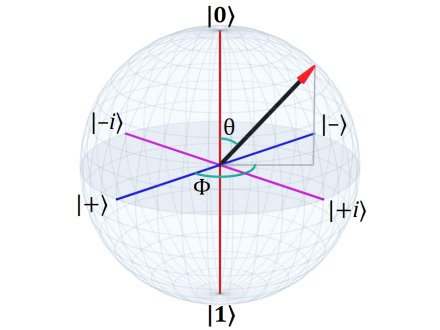
\includegraphics[scale=0.6]{images/bloch-hdr-440.png}
    \caption{Rappresentazione degli autovettori delle matrici di Pauli sulla sfera di Bloch. Il punto indicato dalla freccia rossa indica un generico qubit.}
    \label{fig:BlochSphere2}
\end{figure}

\noindent Come detto in precedenza, le 3 matrici di Pauli parametrizzano lo spin e i 3 assi della sfera di Bloch possono essere associati allo spin. Considerando lo stato generico $\ket{\psi}$ della \eqref{generic qubit}, possiamo definire lo spin lungo una direzione generica $\vec{\sigma} \cdot \vec{n}$ dove $\vec n = (\cos\phi\sin\theta, \sin\phi\sin\theta, \cos\theta)$:

\begin{equation*}
    \vec{\sigma} \cdot \vec n = \cos\phi\sin\theta \, \sigma_1 + \sin \phi \sin \theta \, \sigma_2 + \cos \theta \, \sigma_3 \, ;
\end{equation*}
così facendo è un semplice esercizio di QM dimostrare che $\ket{\psi}$ è autostato di $\vec{\sigma} \cdot \vec n$ con autovalore 1, ossia $\vec{\sigma} \cdot \vec n \ket{\psi} = \ket{\psi}$. Questo significa che dato uno stato sulla sfera di Bloch, allora esso è anche autostato di spin nella direzione individuata da tale qubit: infatti l'idea fisica alla base della sfera di Bloch è che la direzione arbitraria scelta non è altro che la direzione della quantizzazione dello spin. 

\section{Misurazioni}

\begin{itemize}
    \item \textbf{III Postulato} (\textbf{Regola di Born}):
    \begin{enumerate}
        \item \textbf{Misurazione}: sia $\hat{A}$ un osservabile con autostati $\ket{n}$, ossia $\hat{A} \ket{n} = a_n \ket{n}$. Prendiamo per semplicità $a_n \neq a_m \ \forall \, n \neq m$ (osservabile con autovalori distinti). Consideriamo uno stato generico espanso sugli autostati precedenti: $\ket \psi = \sum_n \alpha_n \ket n$. Allora una misura dell'osservabile $\hat{A}$ produce il valore $a_n$ con probabilità data da $\abs{\alpha_n}^2$ (assumendo lo stato correttamente normalizzato).
        
        \item \textbf{Collasso dello stato}: cosa succede allo stato del sistema dopo la misurazione? Istantaneamente lo stato $\ket \psi$ collassa sull'autostato associato all'autovalore risultante dalla misura. Ad esempio se misurando otteniamo $a_n$ allora $\ket{\psi} \rightarrow \ket{n}$. Effettuando delle misure successive sullo stato si ottiene sempre $\ket{n}$ con probabilità esattamente uguale a 1.  
    \end{enumerate}
\end{itemize}

\begin{esempio}
    Consideriamo per esempio il generico qubit in \eqref{generic qubit} e immaginiamo di voler effettuare delle misurazioni in differenti basi. Supponiamo di voler misurare lo spin lungo $z$ (base $\lbrace \ket{0}, \ket{1} \rbrace$ di $\sigma_3$) e lungo $x$ (base $\lbrace \ket{+}, \ket{-} \rbrace$ di $\sigma_1$). Essendo il qubit già decomposto sulla base computazionale, una misurazione lungo $z$ produrrà
    
    \begin{equation*}
        P(\ket{0}) = \abs{\cos \! \left( \frac{\theta}{2} \right)}^2 \, , \qquad P(\ket{1}) = \abs{\sin \! \left( \frac{\theta}{2} \right)}^2 \, .
    \end{equation*}
    
    \noindent Per capire il risultato della misurazione lungo $x$, invece, dobbiamo espandere $\ket{\psi}$ sulla base $\lbrace \ket{+}, \ket{-} \rbrace$: usando le \eqref{basi_di_sigma_12} per esprimere $\lbrace \ket{0}, \ket{1} \rbrace$ in termini di $\lbrace \ket{+}, \ket{-} \rbrace$ ricaviamo
    
    \begin{equation*}
        P(\ket{+}) = \frac{1}{2} \abs{\cos \! \left( \frac{\theta}{2} \right) + e^{i \phi} \sin \! \left( \frac{\theta}{2} \right)}^2 \, , \qquad P(\ket{-}) = \frac{1}{2} \abs{\cos \! \left( \frac{\theta}{2} \right) - e^{i \phi} \sin \! \left( \frac{\theta}{2} \right)}^2 \, .
    \end{equation*}
    
    \noindent Si noti come in entrambe le situazioni la probabilità risulta correttamente normalizzata: $P(\ket{0}) + P(\ket{1}) = P(\ket{+}) + P(\ket{-}) = 1$. 
\end{esempio}

\begin{esempio}
    Consideriamo lo stato $\ket{+}$ delle \eqref{basi_di_sigma_12}. Qual è l'interpretazione fisica di tale stato? Supponiamo che rappresenti lo spin di una particella: quando lo spin si trova in $\ket{+}$ allora sappiamo con certezza che punta lungo la direzione $x$, ossia $P(\ket{+}) = 1$. Al contrario, per una misurazione lungo $z$ sappiamo che $P(\ket{0}) = 1/2$ e $P(\ket{1}) = 1/2$: abbiamo la certezza del risultato lungo l'asse $x$, ma lungo l'asse $z$ si ha totale incertezza. Questo fenomeno è dovuto alla non commutatività degli operatori di spin nelle 3 direzioni:
    
    \begin{equation*}
        \comm{\hat{S}_i}{\hat{S}_j} = i \hbar \varepsilon_{ijk} \hat{S}_k \, .
    \end{equation*}
    
    \noindent Se consideriamo infatti il sistema preparato in $\ket{+}$ e supponiamo di effettuare una misura lungo $z$ ottenendo $\ket{0}$ allora lo stato collasserà in $\ket{0}$ e, d'ora in avanti, qualsiasi misurazione lungo $z$ produrrà sempre $\ket{0}$ con $P(\ket{0}) = 1$. Nonostante ciò, il fatto che $\hat{S}_z$ non commuti con $\hat{S}_x$ fa sì che una misura successiva lungo $x$ "rigeneri" dell'incertezza: $P(\ket{+}) = 1/2$ e $P(\ket{-}) = 1/2$ (si veda $\ket{0}$ espresso in termini di $\lbrace \ket{+}, \ket{-} \rbrace$ dalle \eqref{basi_di_sigma_12}). 
\end{esempio}

\noindent Discutiamo la generalizzazione del III postulato nel caso in cui alcuni autovalori associati ad autostati differenti siano uguali, cioè siamo in presenza di \textbf{degenerazione}. Per esempio supponiamo il caso $N = \dim \mathcal{H} = 6$: 

\begin{equation*}
    \ket \psi = \alpha_1 \ket 1 + \alpha_2 \ket 2 + \alpha_3 \ket 3 + \alpha_4 \ket 4 + \alpha_5 \ket 5 + \alpha_6 \ket 6 \, , 
\end{equation*}

\noindent dove supponiamo la degenerazione su $a_1 = a_2$ e $a_4 = a_5 = a_6$. Introduciamo gli operatori $\hat{P}_{a_i}$ che considerano solamente la parte di $\ket{\psi}$ corrispondente all'autospazio associato ad $a_i$:

\begin{equation*}
    \ket \psi = \underbrace{\alpha_1 \ket 1 + \alpha_2 \ket 2 }_{\hat P_{a_1} \ket \psi} + \underbrace{\alpha_3 \ket 3}_{\hat P_{a_3} \ket \psi} + \underbrace{\alpha_4 \ket 4 + \alpha_5 \ket 5 + \alpha_6 \ket 6}_{\hat P_{a_4 \ket \psi}} \, ;
\end{equation*}

\noindent tali operatori prendono il nome di \textbf{proiettori} e soddisfano le proprietà seguenti:  
\begin{enumerate}
    \item $\hat P_{a_i}^\dagger = \hat P_{a_i}$;
    \item $\hat P_{a_i}^2 = \hat P_{a_i}$;
    \item $\sum_i \hat P_{a_i} = \mathbb{I}$. 
\end{enumerate}

\noindent I proiettori sono utili per scrivere la \textbf{regola di Born} (III postulato) nel caso generale: dato uno stato $\ket{\psi}$ con degenerazione sugli autovalori $a_i$, la probabilità di ottenere il risultato $a_n$ è

\begin{equation*}
    P(a_n) = \norm{\hat{P}_{a_n} \ket{\psi}}^2 \, ;
\end{equation*}

\noindent dopo la misura, la funzione d'onda collassa nel seguente stato normalizzato:

\begin{equation*}
    \ket{\psi} \rightarrow \frac{\hat{P}_{a_n} \ket{\psi}}{\norm{\hat{P}_{a_n} \ket{\psi}}} \, .
\end{equation*}

\noindent Ad esempio, nel caso dello stato sopra scritto, la probabilità di ottenere $a_1 = a_2$ non è altro che 

\begin{equation*}
    P(a_1) = \norm{\hat{P}_{a_1} \ket{\psi}}^2 = \norm{\alpha_1 \ket{1} + \alpha_2 \ket{2}}^2 = \abs{\alpha_1}^2 + \abs{\alpha_2}^2 \, ,
\end{equation*}

\noindent e lo stato collassa in

\begin{equation*}
    \ket{\psi} \rightarrow \frac{\alpha_1 \ket{1} + \alpha_2 \ket{2}}{\sqrt{\abs{\alpha_1}^2 + \abs{\alpha_2}^2}} \, ;
\end{equation*}

\noindent si noti che si ha ancora incertezza su in quale stato si trovi $\ket{\psi}$, ma con un esperimento successivo \textbf{diverso} siamo in grado di risolvere la degenerazione e ottenere $\ket{1}$ o $\ket{2}$. 

\section{Evoluzione temporale}
Il postulato successivo riguarda l'evoluzione temporale degli stati:

\begin{itemize}
    \item \textbf{IV Postulato} (\textbf{Evoluzione temporale}): L'evoluzione temporale di uno stato generico $\ket{\psi(0)}$ è descritta dall'equazione di Schrödinger:
    
    \begin{equation*}
        i \hbar \dv{t} \ket{\psi(t)} = \hat H \ket{\psi(t)} \, ,
    \end{equation*}
    
    \noindent dove $\hat{H}$ è l'operatore (hermitiano) \textbf{hamiltoniana} del sistema. L'equazione di Schrödinger conserva le probabilità: $\braket{\psi(t)} = \braket{\psi(0)} = 1$. 
\end{itemize}

\noindent Solitamente si risolve questa equazione introducendo l'\textbf{operatore di evoluzione temporale} $\hat{U}(t)$:

\begin{equation*}
    \ket{\psi(t)} = \hat{U}(t) \ket{\psi(0)} \, ;
\end{equation*}

\noindent quando l'hamiltoniana è indipendente dal tempo, $\hat{U}(t)$ diventa semplicemente

\begin{equation*}
    \hat{U} (t) = e^{-\frac{i}{\hbar} \hat H t} \, ;
\end{equation*}

\noindent se invece $\hat H = \hat H(t)$, è necessario distinguere i casi di hamiltoniane commutanti o non commutanti a tempi differenti.\\
\noindent Come detto sopra, l'evoluzione temporale preserva le probabilità e ciò è una diretta conseguenza del fatto che $\hat{U}(t)$ sia \textbf{unitario}: 
\begin{itemize}
    \item $\hat U \hat U^\dagger = \hat U^\dagger U = \mathbb{I} \quad \Rightarrow \quad \hat{U}^\dagger = \hat{U}^{-1}$.
    \item Il prodotto scalare è conservato: $\braket{\hat U\phi}{\hat U\psi} = \braket{\phi}{\hat U^\dagger \hat U\psi} = \braket{\phi}{\psi}$. 
\end{itemize}
\noindent Notiamo che $\hat{U}(t)$ per hamiltoniane indipendenti da $t$ è effettivamente unitario:

\begin{equation*}
    \hat U^\dagger \hat U = \left( e^{-\frac{i}{\hbar} \hat H t} \right)^\dagger e^{-\frac{i}{\hbar} \hat H t} = e^{\frac{i}{\hbar} \hat H t} e^{-\frac{i}{\hbar} \hat H t} = \mathbb{I} \, .
\end{equation*}

\section{Gate}\label{sec:gate}

\begin{definizione}[\textbf{Porte quantistiche}]
    L'analogo quantistico delle porte (o gate) logiche classiche sono le \textbf{porte quantistiche} (o \textbf{gate quantistici}). Un gate quantistico è un operatore unitario che cambia lo stato del sistema.
\end{definizione}

\noindent Notiamo che una delle principali differenze che rendono di difficile implementazione le porte quantistiche risiede nel fatto che non possiamo implementare direttamente le più semplici operazioni classiche come \texttt{AND}, \texttt{OR} o \texttt{XOR}. 

\begin{definizione}[\textbf{Circuito Quantistico}]
    Un \textbf{circuito quantistico} è un modello di computazione quantistica in cui una sequenza ordinata di gate quantistici è applicata ai qubit.
\end{definizione}

\noindent In un circuito classico l'uso dei gate logici è banale. Supponiamo di considerare un bit che si trova in 0 o 1: un gate costituisce l'implementazione di un agente esterno che cambia lo stato del bit. Si pensi ad esempio al gate \texttt{NOT} per il quale $a \rightarrow$ \texttt{NOT} $a$:
\begin{center}
    \begin{circuitikz}
        \draw
        (0,4.5) node[not port] (mynot) {}
        (mynot.in) node[left = .4cm, anchor=east] (a) {$0$}
        (mynot.out) node[right = .4cm,anchor=west] (b) {$1 \, ,$}
        (mynot.in) -- (a)
        (mynot.out) -- (b);
    \end{circuitikz}
    $\qquad$
    \begin{circuitikz}
        \draw
        (0,4.5) node[not port] (mynot) {}
        (mynot.in) node[left = .4cm, anchor=east] (a) {$1$}
        (mynot.out) node[right = .4cm,anchor=west] (b) {$0 \, ,$}
        (mynot.in) -- (a)
        (mynot.out) -- (b);
    \end{circuitikz}
\end{center}

\noindent Nel caso invece di un qubit, i circuiti funzionano diversamente perché le porte agiscono su sistemi a due livelli. Immaginiamo che a causa di un agente esterno il qubit $\ket{\psi}$ subisca un evoluzione temporale $\hat{U}$: rappresentiamo questo fatto mediante il circuito seguente
\begin{center}
    \mbox{
        \Qcircuit @C=2em @R=2em {
            \lstick{\ket{\psi}} & \gate{\hat{U}} & \rstick{\hat{U} \ket{\psi} \, ,} \qw \\
        }
    }
\end{center}

\noindent Si ricordi che $\hat{U}$ è sempre un operatore unitario: ad esempio per un'hamiltoniana indipendente dal tempo si ha semplicemente $\hat{U}(t) = e^{-\frac{i}{\hbar}\hat H t}$. \\
\noindent Consideriamo le matrici di Pauli: sappiamo che sono hermitiane ($\sigma^\dagger_i = \sigma_i$) e che soddisfano la proprietà $\sigma_i^2 = \mathbb{I}$, ma questo significa che sono anche matrici unitarie. Questo fatto ci permette di costruire\footnote{Un tale sistema in natura è abbastanza semplice da implementare poiché, essendo $\hat{H} = \vec{\sigma} \cdot \vec B$ l'accoppiamento tra spin e campo magnetico, è facile costruire una tale evoluzione temporale.} dei gate in cui $\hat{U} = \hat{\sigma}_i$.  Ad esempio è possibile implementare dei gate come $\mathbb{I}$, $\sigma_1 \equiv X$, $\sigma_2 \equiv Y$ e $\sigma_3 \equiv Z$. Ricordando che $\sigma_i \sigma_j = i \varepsilon_{ijk} \sigma_k$ per $i \neq j$, notiamo che $XZ = - i Y$ e inoltre anche la matrice $-iY$ è unitaria. Per tale ragione molto spesso, al posto di considerare i gate $\lbrace \mathbb{I}, X, Y, Z \rbrace$ si sceglie la base $\lbrace \mathbb{I}, X, Z, XZ \rbrace$: questo significa che possiamo implementare i gate seguenti
\begin{center}
    \mbox{
        \Qcircuit @C=2em @R=2em {
            & \gate{X} & \qw \\
        }
    } 
    , \ \ \ \ 
    \mbox{
        \Qcircuit @C=2em @R=2em {
            & \gate{Z} & \qw \\
        }
    }
    , \ \ \ \ 
    \mbox{
        \Qcircuit @C=2em @R=2em {
            & \gate{XZ} & \qw \\
        }
    }
    ,
\end{center}

\noindent Consideriamo l'\texttt{X-gate}: dalle \eqref{Pauli_matrices} è evidente che $X$ rappresenta una sorta di "quantum" \texttt{NOT} perché inverte semplicemente lo stato della base computazionale:
\begin{center}
    \mbox{
        \Qcircuit @C=2em @R=2em {
            \lstick{\ket{0}} & \gate{X} & \rstick{\ket{1} \, ,} \qw \\
        }
    } 
    \\
    \mbox{
        \Qcircuit @C=2em @R=2em {
            \lstick{\ket{1}} & \gate{X} & \rstick{\ket{0} \, ,} \qw \\
        }
    }
\end{center}

\noindent Consideriamo ora lo \texttt{Z-gate}: gli stati della base computazionale sono autovettori con autovalori 1 e $-1$ di $\sigma_3$, quindi questo gate inverte semplicemente il segno
\begin{center}
    \mbox{
        \Qcircuit @C=2em @R=2em {
            \lstick{\ket{0}} & \gate{Z} & \rstick{\ket{0} \, ,} \qw \\
        }
    } 
    \\
    \mbox{
        \Qcircuit @C=2em @R=2em {
            \lstick{\ket{1}} & \gate{Z} & \rstick{-\ket{1} \, ,} \qw \\
        }
    }
\end{center}
L'azione dello \texttt{Z-gate} su un generico qubit risulterà quindi in
\begin{center}
    \mbox{
        \Qcircuit @C=2em @R=2em {
            \lstick{a \ket{0} + b \ket{1}} & \gate{Z} & \rstick{a \ket{0} - b \ket{1} \, ,} \qw \\
        }
    } 
\end{center}
e questo significa che $Z$ aggiunge semplicemente una fase $e^{i \pi} = -1$ allo stato. Ricapitolando: l'\texttt{X-gate} implementa un'interferenza dall'esterno che inverte lo stato (ad esempio cambia segno dello spin lungo $z$) e lo \texttt{Z-gate} implementa l'introduzione di una fase. \\
\noindent Una matrice particolarmente importante per i nostri scopi è 
\begin{equation}\label{Hadamard_matrix}
    H = \frac{1}{\sqrt{2}} 
    \begin{pmatrix}
        1 & 1 \\ 1 & -1 
    \end{pmatrix} \, , 
\end{equation}
chiamata \textbf{matrice di Hadamard}. Notiamo che è unitaria in quanto $H^\dagger H = \mathbb{I}$. Essa può essere implementata nel cosiddetto \texttt{H-gate} o \textbf{gate di Hadamard}: si tratta di un gate particolarmente importante (lo useremo largamente durante tutto il corso) in quanto permette di cambiare base $\lbrace \ket{0}, \ket{1} \rbrace \leftrightarrow \lbrace \ket{+}, \ket{-} \rbrace$ 

\begin{center}
    \mbox{
        \Qcircuit @C=2em @R=2em {
            \lstick{\ket{0}} & \gate{H} & \rstick{\ket{+} \, ,} \qw \\
        }
        \ \ \ \ \ \ \ \ \ \ \ \ \ \ \ \ \ \ \ \ 
        \Qcircuit @C=2em @R=2em {
            \lstick{\ket{+}} & \gate{H} & \rstick{\ket{0}\, ,} \qw \\
        }
    }
    \\
    \mbox{
        \Qcircuit @C=2em @R=2em {
            \lstick{\ket{1}} & \gate{H} & \rstick{\ket{-} \, ,} \qw \\
        } 
        \ \ \ \ \ \ \ \ \ \ \ \ \ \ \ \ \ \ \ \ 
        \Qcircuit @C=2em @R=2em {
            \lstick{\ket{-}} & \gate{H} & \rstick{\ket{1} \, ,} \qw \\
        }
    }
\end{center}

\noindent Possiamo introdurre anche le matrici seguenti (ci serviranno più avanti)

\begin{equation}\label{S_T_matrices}
    S \equiv \sqrt{Z} =
\begin{pmatrix}
    1 & 0 \\ 0 & i
\end{pmatrix} \, , \qquad 
T \equiv \sqrt{S} =
\begin{pmatrix}
    1 & 0 \\ 0 & e^{i \frac{\pi}{4}}
\end{pmatrix} \, ,
\end{equation}

\noindent Le matrici introdotte in precedenza costituiscono gli oggetti base con cui andremo a implementare diversi gate e circuiti durante tutto il corso. Per costruire il gate più generale possiamo esponenziare scrivendo $U = e^{-\frac{i}{\hbar} H t}$ dove $H = a \mathbb{I} + b_i \sigma_i$ e $a, b_i \in \mathbb{R}$ con $i = 1,2,3$. Esiste una particolare classe di operatori che utilizzeremo molto dati da
\begin{equation*}
    R_{\vec{n}}(\lambda) = e^{-i \frac{\lambda}{2} (\vec n \cdot \vec \sigma)} \, ;
\end{equation*}
si tratta di un caso particolare dell'esponenziazione precedente in cui $a = 0$ e i coefficienti $b_i$ sono scelti lungo un particolare versore $\vec n$. Questo operatore unitario implementa una rotazione di angolo $\lambda$ attorno alla direzione individuata da $\vec n$:

\begin{equation}\label{rotation_n_lambda}
    R_{\vec{n}}(\lambda) = e^{-i \frac{\lambda}{2} (\vec n \cdot \vec \sigma)} = \cos \! \left( \frac{\lambda}{2} \right) \mathbb{I} - i \sin \! \left( \frac{\lambda}{2} \right) \vec \sigma \cdot \vec n \, ;
\end{equation}
(si espanda il LHS con la serie di Taylor dell'esponenziale e si usi $(\vec \sigma \cdot \vec n)^2 = \mathbb{I}$ per dimostrare l'uguaglianza con il RHS). È possibile dimostrare, inoltre, che qualsiasi matrice unitaria $2 \times 2$ può essere scritta nella forma seguente
\begin{equation}\label{general_2by2_matrix}
    U = e^{i \alpha}
    \begin{pmatrix}
        e^{-i \frac{\beta}{2}} & 0 \\ 0 & e^{i \frac{\beta}{2}}
    \end{pmatrix}
    \begin{pmatrix}
        \cos \frac{\gamma}{2} & - \sin \frac{\gamma}{2} \\ \sin  \frac{\gamma}{2} & \cos \frac{\gamma}{2}
    \end{pmatrix}
    \begin{pmatrix}
        e^{-i \frac{\delta}{2}} & 0 \\ 0 & e^{i \frac{\delta}{2}}
    \end{pmatrix}
    = e^{i \alpha} R_z(\beta) R_x(\gamma) R_z(\delta) \, ; 
\end{equation}
perciò il più generale operatore unitario presenta 4 parametri reali $\alpha, \beta, \gamma, \delta \in \mathbb{R}$ e può implementare un possibile gate in un computer quantistico. Appare subito evidente come la scelta di 4 possibili parametri reali (quindi continui) consenta di realizzare un numero nettamente maggiore di gate logici quantistici rispetto al caso dei gate logici classici. 
    \vspace{1cm}
\newline
\lecture{3}{14/10/2021}
\vspace{0.5cm}
\noindent Abbiamo visto come sia possibile calcolare il valore di aspettazione di $\expval{A}$ a partire dalle funzioni d'onda. Vogliamo vedere come sia possibile sfruttare la matrice densità per ottenere il medesimo risultato. Cominciamo considerando il generico insieme di stati $\{p_i, \ket{\psi_i}\}$ e la matrice densità corrispondente $\hat \rho=\sum_i p_i\op{\psi_i}{\psi_i}$. Per il singolo stato $\ket{\psi_i}$ avevamo visto che
\begin{equation*}
    \begin{aligned}
        \expval{A}_{\psi_i} &= \sum_k p_k a_k \\
                            &= \sum_k \ip{\psi_i}{a_k}\ip{a_k}{\psi_i}a_k \\
                            &= \bra{\psi_i}\sum_k a_k \ket{a_k}\ip{a_k}{\psi_i} \\
                            &= \expval{A}{\psi_i}
    \end{aligned}
\end{equation*}
Tuttavia, nel caso della matrice densità, abbiamo un insieme di funzioni d'onda, per cui
\begin{equation*}
    \begin{aligned}
        \expval{A} &= \sum_i p_i \expval{\hat A}{\psi_i} \\
                   &= \sum_i p_i \Tr \left(\hat A\op{\psi_i}{\psi_i}\right) \\
                   &= \Tr \left(A\sum_i p_i \op{\psi_i}{\psi_i}\right) \\
                   &= \Tr\left(\hat A\rho\right) \, .
    \end{aligned}
\end{equation*}

\subsection*{Equazione di von-Neumann - Liouville}
Per il \textbf{IV Postulato}, riguardante l'evoluzione temporale, la matrice densità evolve come $\hat U \hat \rho \hat U^\dagger$, ci chiediamo se sia possibile realizzare un'equazione analoga a quella di Schrödinger per la matrice densità. La risposta è affermativa, infatti
\begin{equation*}
    \begin{aligned}
        \derivative{\hat \rho}{t} &= \sum_i p_i\left(\derivative{\ket{\psi_i}}{t}\bra{\psi_i}+\ket{\psi_i}\derivative{\bra{\psi_i}}{t}\right) \\
                                  &= \sum_i \frac{p_i}{i\hbar}\left(\hat H \op{\psi_i}{\psi_i}-\op{\psi_i}{\psi_i}\hat H\right) \\
                                  &= \frac{1}{i\hbar}\comm{\hat H}{\hat \rho}
    \end{aligned}
\end{equation*}

\noindent Consideriamo ora un paio di esempi per assodare i concetti finora trattati
\begin{esempio}
    Consideriamo un qubit nella base computazionale $\{\ket 0, \ket 1\}$ oppure possiamo pensare di prendere la base
    \begin{equation*}
        \ket a = \frac{\ket 0 +\ket 1}{\sqrt 2} \,
    \end{equation*}
    \begin{equation*}
        \ket b = \frac{\ket 0 -\ket 1}{\sqrt 2} \, ;
    \end{equation*}
    entrambe le basi sono degli stati puri.\\
    Consideriamo lo stato $\ket a$ e costruiamo la matrice densità per la base computazionale
    \begin{equation*}
        \hat \rho = \frac 12 \op{0}{0} + \frac 12 \op{1}{1} \, ,
    \end{equation*}
    come possiamo notare, gli stati hanno la medesima probabilità. Ora possiamo fare una \textbf{projective measurament} definendo i proiettori:
    \begin{itemize}
        \item $\hat P_0=\op{0}{0}$;
        \item $\hat P_1=\op{1}{1}$;
        \item $\hat P_a=\op{a}{a}$.
    \end{itemize}
    Andiamo a misurare le probabilità di misurare $\ket 0$ e $\ket 1$ sullo stato $\ket a$:
    \begin{equation*}
        p(\ket 0)=\mel{a}{\hat P_0}{a}=\frac 12 \quad \, , \quad p(\ket 1)=\mel{a}{\hat P_1}{a}=\frac 12 \, .
    \end{equation*}
    Cosa succede se consideriamo $\rho$?
    \begin{equation*}
        p(\ket 0)=\mel{0}{\hat \rho}{0}=\frac 12 \quad \, , \quad p(\ket 1)=\mel{1}{\hat \rho}{1}=\frac 12 \, .
    \end{equation*}
    Come possiamo notare otteniamo in entrambi i casi la medesima probabilità, se invece andassimo a misurare $\ket a$?
    \begin{equation*}
        \begin{aligned}
            p(\ket a) &= \mel{a}{\hat P_a}{a} \\
                      &= \ip{a}{a}\ip{a}{a} \\
                      &= 1 \, .
        \end{aligned}
    \end{equation*}
    Per quanto riguarda la matrice densità
    \begin{equation*}
        \begin{aligned}
            p(\ket a) &= \mel{a}{\hat \rho}{a} \\
                      &= \Tr \left(\hat \rho \op{a}{a}\right) \\
                      &= \frac 12 \, .
        \end{aligned}
    \end{equation*}
    In questo caso, misurare in un altra base ci dà due risultati differenti.
\end{esempio}
\noindent Questo esempio in realtà lo possiamo incontrare, dal punto di vista pratico, se ci addentriamo nello studio dello spin di un elettrone in un atomo (esperimento di Stern-Gerlach) oppure nella trattazione della polarizzazione di un fotone.

\noindent In generale noi possiamo scrivere la matrice densità in una base e poi riscriverla in un secondo momento in un'altra base
\begin{equation*}
    \hat \rho = \sum_k \omega_k \op{\psi_k}{\psi_k} \, ,
\end{equation*}
dove 
\begin{equation*}
    \{\omega_k, \ket{\psi_k}\} \quad \text{e} \quad \ket{\psi_k}=\sum_j a_j^k \ket{a_j} \, .
\end{equation*}
Nella nuova base, la matrice densità sarà
\begin{equation*}
    \begin{aligned}
        \hat \rho &= \sum_k {\omega_k}\left(\sum_j a_j^k \ket{a_j}\right)\left(\sum_i a_i^{*k}\bra{a_i}\right) \\
             &= \sum_{k,j,i} \omega_k a_j^ka_i^{*k}\op{a_j}{a_i}
    \end{aligned}
\end{equation*}
per cui gli elementi di matrice saranno
\begin{equation*}
    \begin{aligned}
        \rho_{mn} &= \mel{a_m}{\hat \rho}{a_n} \\
                       &= \sum_k \omega_k a_m^ka_n^{*k}
    \end{aligned}
\end{equation*}
e gli elementi sulla diagonale
\begin{equation*}
    \rho_{nn}=\sum_k\omega_k \abs{a_n^k}^2
\end{equation*}

\subsection{POVM: Misura a valori operatoriali positivi}
Molti tipi di misurazione, come ad esempio la rivelazione della posizione di un fotone, non possono essere visti come proiezioni perché lo stato dopo la misura viene distrutto. Nel caso considerato, quando misuriamo il fotone esso viene assorbito dal rivelatore e non esiste più. A differenza delle misure proiettive non posso effettuare un'ulteriore misura sullo stesso stato. La proiezione non permette inoltre di distinguere in maniera esatta due stati non ortogonali. Ad esempio presi due stati $\ket \psi$ e $\ket \phi$, se sono tra loro ortogonali sarà facile distinguerli con i proiettori, ma se non sono ortogonali non possiamo distinguerli e gli unici risultati che possiamo dare sono:
\begin{itemize}
    \item È nello stato $\ket \psi$;
    \item È nello stato $\ket \phi$;
    \item O in qualcos'altro.
\end{itemize}
Una misura a valori operatoriali positivi (POVM) è una misura i cui valori sono operatori semi-definiti positivi su uno spazio di Hilbert che non richiedono ortogonalità, cioè non soddisfano la terza proprietà che abbiamo visto quando abbiamo introdotto i proiettori: $\hat P_i \hat P_j = \hat P_i\delta_{ij}$. La POVM può essere utile per classificare uno stato con 3 possibili identificazioni (come $\ket \psi$, $\ket \phi$ o "non so") dove invece una misura proiettiva è inutile.

\subsection{Cambi di base: stati puri e miscele}

\noindent Supponiamo di avere una matrice densità $\hat \rho=\sum_i p_i \op{\psi_i}{\psi_i}$ e un'osservabile $\hat A$ ($\ket {a_k}$, $a_k$). Vogliamo valutare il valore di aspettazione di questa osservabile:
\begin{equation*}
    \begin{aligned}
        \expval{A} &= \Tr\left(\hat\rho \hat A\right) \\
                   &= \Tr\left(\sum_{ijk} \rho_{ij}\op{a_i}{a_j}a_k\op{a_k}{a_k}\right) \\
                   &= \sum_{ik}\rho_{ik}a_k\Tr\left(\op{a_i}{a_k}\right) \\
                   &= \sum_{ik}\rho_{ik}a_k\ip{a_k}{a_i} \\
                   &= \sum_k\rho_{kk}a_k
    \end{aligned}
\end{equation*}
Quindi, solo i $\rho_{kk}=\mel{a_k}{\rho}{a_k}$ sono necessari per calcolare il valore di aspettazione e gli elementi off-diagonal nella nostra rappresentazione sono apparentemente inutili. Tuttavia, gli elementi off-diagonal spesso ci dicono se la matrice corrisponde a uno stato puro o meno. Se abbiamo una matrice di densità non diagonale in una base di un'osservabile, anche se il valore di aspettazione dell'osservabile stessa è dato solo dagli elementi diagonali, se gli elementi off-diagonal sono diversi da zero allora lo stato può essere puro, poiché la matrice diagonalizzata può avere tutte le voci uguali a $0$, tranne una uguale a $1$. Questi elementi fuori diagonale sono chiamati coerenza della matrice densità. Per esempio, consideriamo la seguente matrice $2\times 2$
\begin{equation*}
    \begin{pmatrix}
        a & c \\
        c^* & b
    \end{pmatrix}
\end{equation*}
I coefficienti $c$ e $c^*$ prendono il nome di \textbf{coerenze}, questo perché:
\begin{itemize}
    \item Se $c=c^*=0$, allora abbiamo una miscela di stati;
    \item Se $c,c^*\neq 0$, allora possiamo avere uno stato puro, in quanto la matrice può essere diagonalizzata nella forma
        \begin{equation*}
            \begin{pmatrix}
                1 & 0 \\
                0 & 0
            \end{pmatrix}
        \end{equation*}
\end{itemize}
Osserviamo che, generalmente, $c$ e $c^*$ seguono una legge di decadimento, per cui scalano come $e^{-t/T_1}$, il che significa che lo stato sta perdendo la sua purezza al passare del tempo. Questo è uno dei problemi più importanti quando si lavora con dei sistemi come i qubit, in quanto ne limita il suo utilizzo.
    \vspace{1cm}
\newline
\lecture{4}{14/10/2021}
\vspace{0.5cm}
\section{Sfera di Bloch}
Esiste un modo di rappresentare lo stato di un qubit, in maniera grafica, attraverso l'utilizzo della \textbf{sfera di Bloch}. Questo espediente è comodo per comprendere che cosa sta avvenendo allo stato di un qubit, lo svantaggio principale riguarda la sua applicabilità, in quanto è possibile usarlo per singoli qubit. Come al solito noi utilizziamo la matrice densità $\hat \rho$ piuttosto che la funzione d'onda $\psi$ per descrivere lo stato di un sistema a due livelli\footnote{Nel caso di un qubit, la matrice densità è rappresentata da una matrice $2\times2$}:
\begin{equation*}
    \hat \rho = \begin{pmatrix}
                    \rho_{00} & \rho_{01} \\
                    \rho_{10} & \rho_{11}
                \end{pmatrix} \, ,
\end{equation*}
dove $\rho_{00}$, $\rho_{11} \in \mathbb{R}$, $\rho_{11}=1-\rho_{00}$ e $\rho_{01}=\rho_{10}^*$. A questo punto ridefiniamo gli elementi di $\hat \rho$ come
\begin{equation*}
    \rho_{00}=\alpha \quad \, , \quad \rho_{11}=1-\alpha \quad \, , \quad \rho_{01}=\beta + i\gamma \quad \, , \quad \rho_{10}=\beta - i \gamma
\end{equation*}
dove $\alpha, \beta$ e $\gamma \in \mathbb{R}$. \\
Se consideriamo l'insieme di matrici dato dall'identità e dalle matrici di Pauli $\{\mathbb{I}, \sigma_1, \sigma_2, \sigma_3 \}$ possiamo riscrivere la matrice densità in una forma particolarmente interessante
\begin{equation*}
    \hat \rho = a\mathbb{I} + \sum_{i=1}^3 c_i\sigma_i \, ,
\end{equation*}
siccome $\Tr(\hat \rho)\overset{!}{=}1$, allora dal momento che $\Tr(\sigma_i)=0$ e $\Tr(\mathbb{I})=2$ abbiamo che $a=\frac 12$.
\begin{equation*}
    \hat \rho = \frac 12\left(\mathbb{I}+\sum_{i=1}^3 p_i \sigma_i\right) \, .
\end{equation*}
Cosa sono i $p_i$? Osserviamo che $\Tr(\hat \rho \sigma_i)=p_i=\expval{\sigma_i}$, cioè corrispondono ai valori di aspettazione della corrispondente matrice di Pauli tracciata insieme alla matrice densità.\\
A questo punto possiamo prendere i $p_i$ come le componenti di un vettore $\vec{p}=(p_1, p_2, p_3)$ che si trova all'interno della sfera di Bloch come possiamo vedere in Figura \ref{fig:BlochSphere}.
In particolare notiamo che
\begin{itemize}
    \item Se $\hat \rho$ è \textbf{puro}, $\hat \rho=\op{\psi}{\psi}$, dove
    \begin{equation*}
        \ket \psi = \cos \frac \theta 2 \ket 0 + e^{i\phi}\sin \frac \theta 2 \ket 1
    \end{equation*}
    $\hat \rho$ e $\psi$ rappresentano lo stesso stato sulla sfera di Bloch, è situato sulla superficie della sfera;
    \item Se $\hat \rho$ è una \textbf{miscela}
    \begin{equation*}
        \hat \rho = \begin{pmatrix}
                        \frac{1+p_z}{2} & \frac{p_x-ip_y}{2} \\
                        \frac{p_x+ip_y}{2} & \frac{1-p_z}{2}
                    \end{pmatrix}
    \end{equation*}
    e calcolassimo $\rho^2$ e poi $\Tr(\rho^2)$ troveremo che
    \begin{equation*}
        \rho^2 = \frac 14 \left(\mathbb{I}+\sum_ip_i \sigma_i + \sum_j p_j \sigma_j + \sum_{ij}p_ip_j\sigma_i\sigma_j\right)
    \end{equation*}
    \begin{equation*}
        \Tr(\rho^2) = \frac 12 + \frac 24 \sum_i p_i^2=\frac 12 \left(1+ \abs{\vec p}^2\right)
    \end{equation*}
    Se $\abs{\vec p}^2$ è minore di 1 allora abbiamo una miscela, la sfera che si ottiene da $\vec p$ è una sfera all'interno di quella unitaria (stato puro).
\end{itemize}
\begin{figure}[!ht]
    \centering
    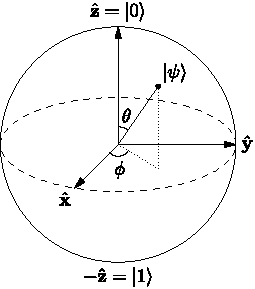
\includegraphics[scale=1.4]{images/Bloch_Sphere.pdf}
    \caption{Rappresentazione generale di un qubit sulla sfera di Bloch.}
    \label{fig:BlochSphere}
\end{figure}
\subsection{Matrice densità termica}
Supponiamo di avere $\hat \rho=\sum_n \omega_n \op{\psi_n}{\psi_n}$, in principio abbiamo molti modi per descrivere il nostro stato da $\ket{\psi_n}$ ognuno con probabilità $\omega_n$. Se il nostro sistema è libero di scambiare energia con l'ambiente abbiamo a che fare con un \textbf{sistema aperto}. Dopo un lungo periodo di tempo di interazione, il nostro sistema raggiungerà un equilibrio, cosicché la nostra probabilità per lo stato $\ket{\psi_n}$ sarà
\begin{equation*}
    \omega_n \equiv \frac{e^{-E_n/k_BT}}{Z} \, ,
\end{equation*}
dove $E_n$ è l'energia dello stato $\ket{\psi_n}$ e $Z=\sum_i e^{-E_i/k_BT}$ è la funzione di partizione canonica.\\
Se prendiamo la base $\ket n$ tale per cui $\hat H \ket n = E_n \ket n$ abbiamo
\begin{equation*}
    \hat \rho = \frac{e^{-\hat H/k_BT}}{Z}\, , \qquad Z=\Tr(e^{-\hat H/k_BT})=1\, , \qquad \rho_{mn}=\mel{m}{\hat \rho}{n}=\frac{e^{-E_n/k_BT}}{Z}\delta_{mn}\equiv \omega_n\, .
\end{equation*}
Usando la base computazionale $\{\ket 0, \ket 1\}$, con energie rispettivamente $E_0$, $E_1$, la matrice densità sarà
\begin{align*}
    \rho &= a_0 \op{0}{0} + a_1 \op{1}{1} \\
         &= \frac{e^{-E_0/k_BT}}{Z}\op{0}{0}+\frac{e^{-E_1/k_BT}}{Z}\op{1}{1}\, ,
\end{align*}
il rapporto tra i due coefficienti è pari a $a_1/a_0=e^{-\Delta E/k_BT}$ quindi possiamo osservare che se
\begin{itemize}
    \item $k_BT \gg \Delta E$, $a_1/a_0 \rightarrow 1$ la matrice densità è una miscela. Il sistema sarà portato allo stato massimamente miscelato (al centro della sfera di Bloch).
    \item $k_BT \ll \Delta E$, $a_1/a_0 \rightarrow 0$, $a_0 \rightarrow 1$ la matrice densità è uno stato puro, poiché il sistema disperde la sua energia nell'ambiente e decade nel suo stato fondamentale.
\end{itemize}
\section{Sistemi compositi}
Utilizziamo sistemi quantistici per studiarne i comportamenti quantistici, per farlo dobbiamo interagire con questi oggetti per misurare qualche loro proprietà, ad esempio sistemi macroscopici, come i rivelatori, interagiscono con sistemi microscopici. Dobbiamo trovare le connessioni che vi sono tra rivelatore e sistema. La terza componente che subentra tra rivelatore e sistema quantistico è l'ambiente, a differenza degli altri due, la sua trattazione è molto complessa per cui rimuoviamo l'ambiente e trattiamo il sistema composito rivelatore e sistema. \\
Trovando un modo di rimuovere l'ambiente dal nostro sistema composito, consideriamo due sistemi descritti rispettivamente da due spazi di Hilbert $\mathcal{H}_1$ e $\mathcal{H}_2$. Il sistema composito è dato da $\mathcal{H}_1\otimes\mathcal{H}_2=\mathcal{H}$. Se $\text{dim}\mathcal{H}_1 = n$ e $\text{dim}\mathcal{H}_2 = m$, allora $\text{dim}\mathcal{H} = n\times m$. Introduciamo l'ultimo postulato della meccanica quantistica
\begin{itemize}
    \item \textbf{V Postulato} (\textbf{Sistemi compositi}): Consideriamo un sistema quantistico composto da 2 sottosistemi $1$ e $2$ con spazi di Hilbert $\mathcal{H}_1$ e $\mathcal{H}_2$ rispettivamente. Lo spazio di Hilbert del sistema totale è dato da\footnote{Il simbolo "$\otimes$" indica il \textbf{prodotto tensoriale} tra spazi.} $\mathcal{H} = \mathcal{H}_1 \otimes \mathcal{H}_2$.
\end{itemize}
Se $\ket{\psi}_1\in\mathcal{H}_1$ e $\ket{\psi}_2\in\mathcal{H}_2$, allora $\ket{\psi}_1\otimes\ket{\psi}_2\in\mathcal{H}$, più precisamente se $\ket{n}_1$ e $\ket{m}_2$ sono una base per $\mathcal{H}_1$ e $\mathcal{H}_2$, allora $\ket{nm}$ è una base per $\mathcal{H}$. \\
Quando $n=m=2$, allora $\ket{nm}=\{\ket{00}, \ket{01}, \ket{10}, \ket{11}\}$ e $\ket \psi \in \mathcal{H}$ è scrivibile come $\ket{\psi}=\sum_{n,m}a_{nm}\ket{nm}$. \\
Introduciamo gli \textbf{stati separabili}, come suggerisce il nome si tratta di stati che possono essere trattati separatamente e si possono combinare le rispettive soluzioni in un secondo momento, infatti
\begin{equation*}
    \underbrace{\ket{\psi_1}}_{= \ket 0, \ket 1}\otimes\underbrace{\ket{\psi_2}}_{= \ket 0, \ket 1}=\alpha a \ket{00} + \alpha b \ket{01} + \beta a \ket{10} + \beta b \ket{11}
\end{equation*}
Accanto agli stati, abbiamo gli operatori che lavorano in questo spazio $\mathcal{H}$, per esempio se $\hat A \in L(\mathcal{H}_1)$, $\hat B \in L(\mathcal{H}_1)$, allora $\hat U = \hat A \otimes \hat B$. Quest'ultimo operatore agisce nel seguente modo
\begin{equation*}
    \hat U \ket \psi = \hat A \otimes \hat B(\ket{\psi_1}\otimes\ket{\psi_2})=\hat A\ket{\psi_1}\otimes \hat B\ket{\psi_2}
\end{equation*}
Perché ci interessa? Perché questi operatori possono essere associati ad osservabili! Come realizziamo una misura su un sistema composito? Supponiamo di avere
\begin{equation*}
    \tilde{A}=A\otimes \mathbb{I} \Rightarrow \tilde{A}: \mathcal{H} \rightarrow \mathcal{H}
\end{equation*}
$\hat A$ rappresenta la misura su un sistema di qubit mentre $\hat B$ l'identità. In questo caso $\hat A$ possiede due proiettori
\begin{equation*}
    P_A^0 = \op{0}{0} \qquad P_A^1=\op{1}{1} \, ,
\end{equation*}
e vogliamo andare a valutare
\begin{equation*}
    \expval{\tilde{A}}=\expval{A\otimes \mathbb{I}}=\mel{\psi}{A \otimes \mathbb{I}}{\psi}=\sum_{ijk}a_{ij}^*a_{kj}\mel{i}{A}{k} \, ,
\end{equation*}
dove ovviamente $\ket \psi \in \mathcal{H}, \ket \psi = \sum_{ij}a_{ij}\ket{ij}$.\\
Otteniamo così
\begin{equation*}
    \expval{\tilde{A}}=\sum_{ij}a_{ij}^2\mel{i}{A}{j} \, .
\end{equation*}
La funzione d'onda che andiamo a considerare è data da $\ket{\psi_1}\otimes\ket{\psi_2}$ e risulta essere definita come
\begin{equation*}
    \ket \psi = \alpha a \ket{00} + \alpha b \ket{01} + \beta a \ket{10} + \beta b \ket{11}\, ,
\end{equation*}
da cui otteniamo che
\begin{align*}
    &\hat A \ket 0 = \ket 0 \\
    &\hat A \ket 1 = -\ket 1 
\end{align*}
cioè
\begin{equation*}
    \hat A = \begin{pmatrix}1 & 0 \\ 0 & -1 \end{pmatrix}
\end{equation*}
e il suo valore di aspettazione è pari a
\begin{equation*}
    \expval{A}=(\alpha a)^2 + (\alpha b)^2 - (\beta a)^2 - (\beta b)^2 \, .
\end{equation*}
Nel caso in cui
\begin{align*}
    &A\otimes\mathbb{I}\left[\frac{\ket{00}+\ket{01}}{\sqrt 2}\right] \Rightarrow \ket{00}, \ket{01} \quad \text{sono stati separabili} \\
    &A\otimes\mathbb{I}\left[\frac{\ket{01}-\ket{10}}{\sqrt 2}\right] \Rightarrow \ket{01}, \ket{10} \quad \text{sono stati entangled} \\
\end{align*}
\subsection{Matrice densità ridotta}
Se abbiamo uno spazio di Hilbert $\mathcal{H}_A$ e misuriamo l'osservabile $\hat A$ ($a_k$, $\ket{a_k}$, abbiamo una probabilità di ottenere il risultato $a_k$ pari a
\begin{equation*}
    p(a_k)=\Tr\left(\op{a_k}{a_k}\rho\right)=\Tr\left(P_{a_k}\rho\right) \, .
\end{equation*}
Altre informazioni che possiamo ottenere sono
\begin{equation*}
    \expval{A}=\Tr(A\rho) \, ,
\end{equation*}
dove
\begin{equation*}
    \rho \rightarrow \frac{P_{a_k}\rho P_{a_k}}{\sqrt{\Tr{P_{a_k}\rho}}} \, ,
\end{equation*}
questo discorso è valido per un qubit. Supponiamo di considerare ora un qubit connesso a un rivelatore, ambiente, \dots In questo caso lo spazio di Hilbert è dato da $\mathcal{H}_A \otimes \mathcal{H}_B$, in questo caso la matrice densità $\rho^{AB}$ è un operatore appartenere a questo spazio. Vogliamo sapere se possiamo ottenere informazioni sul sottospazio $\mathcal{H}_A$, ignorando completamente $\mathcal{H}_B$, la risposta è affermativa e lo si fa nel seguente modo
\begin{equation*}
    \rho^A = \Tr_B(\rho^{AB}) \, ,
\end{equation*}
questa quantità prende il nome di \textbf{matrice densità ridotta}. Cerchiamo di formalizzare meglio questo risultato. \\
Siano $A:\mathcal{H}_A \rightarrow \mathcal{H}_A$ e $B:\mathcal{H}_B \rightarrow \mathcal{H}_B$ due operatori. La loro combinazione è definita come $A \otimes B:\mathcal{H}_A\otimes \mathcal{H}_B \rightarrow \mathcal{H}_A\otimes\mathcal{H}_B$, la \textbf{traccia parziale} è data da
\begin{align*}
    &\Tr_A : L(\mathcal{H}_A\otimes \mathcal{H}_B) \rightarrow L(\mathcal{H_B}) \\
    &\Tr_B : L(\mathcal{H}_A\otimes \mathcal{H}_B) \rightarrow L(\mathcal{H_A}) \, .
\end{align*}
Consideriamo il seguente esempio
\begin{esempio}
Sia $\rho^{AB}=\rho \otimes \sigma$, vogliamo valutare la traccia parziale sul sottospazio $\mathcal{B}$, in questo caso
\begin{equation*}
    \rho^A = \Tr_B(\rho^{AB})=\Tr_B(\rho \otimes \sigma)=\Tr(\sigma)\rho = \rho
\end{equation*}
questo per quanto riguarda \textbf{stati separabili}, ma in generale non è sempre vero! Infatti supponiamo di considerare
\begin{equation*}
    \rho = \frac{\ket{00}+\ket{11}}{\sqrt 2}\frac{\bra{00}+\bra{11}}{\sqrt 2}
\end{equation*}
se eseguissimo la traccia parziale sul sottospazio $\mathcal{H}_2$, avremmo che
\begin{equation*}
    \rho_1 = \Tr_2\rho = \frac{\mathbb{I}}{2}
\end{equation*}
In questo caso, abbiamo sì che $\Tr (\rho_1)=1$, ma $\Tr(\rho_1^2)=\frac 12$, cioè $\rho_1$ è una miscela di stati!
\end{esempio}
    \vspace{0.5cm}
\noindent \lecture{5}{21/10/2021}

\section{Interazione con l'ambiente}

Consideriamo un qubit interagire con l'ambiente. Essendo il qubit un sistema non chiuso, non possiamo descrivere la sua evoluzione temporale come sola evoluzione del qubit. Bisognerà allora tenere in conto della sua interazione con l'ambiente e per farlo possiamo sfruttare la \textbf{matrice densità}. L'equazione del moto per la matrice densità, chiamata \textbf{equazione di Liouville-von Neumann}, segue direttamente dall'equazione di Schrödinger:
\begin{equation}
    \dv{\hat \rho}{t} = \sum_j \dv{t} \left(p_j\op{\psi_j}{\psi_j}\right)=\sum_j p_j\frac{1}{i\hbar}\left(\hat H \op{\psi_j}{\psi_j}-\op{\psi_j}{\psi_j}\hat H\right)=\frac{1}{i\hbar}\comm{\hat H}{\hat \rho} \, .
    \label{eq:liouville-von-neumann}
\end{equation}
L'evoluzione descritta dall'equazione \eqref{eq:liouville-von-neumann} è unitaria e la sua soluzione può essere scritta come
\begin{equation*}
    \hat \rho (t) = \hat U(t)\hat \rho(0) \hat U^\dagger(t) \, .
\end{equation*}
Tuttavia, questo processo descritto dalla \eqref{eq:liouville-von-neumann} non descrive alcun cambiamento sulla sua purezza, infatti quest'ultima risulta essere preservata:
\begin{equation*}
    \hat \xi(t) = \Tr\left(\hat \rho(t)^2\right) = \Tr\left(\hat U(t)\hat \rho(0) \hat U^\dagger(t)\hat U(t)\hat \rho(0) \hat U^\dagger(t)\right)=\Tr\left(\hat \rho (0)^2\right)=\hat \xi(0)
\end{equation*}
Questo significa che l'evoluzione di uno stato pure in una miscela di stati, includendo il processo di misurazione, non può essere descritto dalla \eqref{eq:liouville-von-neumann} ed è un processo essenzialmente non unitario.\\
Per risolvere questo aspetto l'hamiltoniana deve includere più termini
\begin{equation*}
    \hat H = \hat H_S + \hat H_E + \hat H_I \, ,
\end{equation*}
essi sono rispettivamente l'hamiltoniana di sistema, dell'ambiente e di interazione tra sistema e ambiente. Se assumiamo, come è ragionevole, che il sistema non abbia alcun effetto sull'ambiente e che l'hamiltoniana di interazione sia piccola (e quindi possiamo trattarla con la teoria perturbativa) possiamo facilmente studiare l'evoluzione della matrice densità nella rappresentazione d'interazione
\begin{equation*}
    \dv{\hat \rho_{int}}{t}=\frac{1}{i\hbar}\comm{\hat H_{int\,I}(t)}{\hat \rho_{int}(t)} \, ,
\end{equation*}
e
\begin{equation*}
    \hat \rho(t) = \hat \rho (-\infty) + \frac{1}{i\hbar}\int_{-\infty}^t \dd{t'}\comm{\hat H_{I}(t')}{\hat \rho(t')} \, ,
\end{equation*}
dove, supponendo che non solo inizialmente il sistema e l'ambiente fossero statisticamente indipendenti l'uno dall'altro, ma rimarranno tali, possiamo scrivere
\begin{align*}
    \hat \rho(-\infty) &= \hat \rho_S(-\infty)\otimes\hat\rho_E \\
    \hat \rho (t) &= \hat \rho_S(t)\otimes\hat\rho_E \, .
\end{align*}
A questo punto, possiamo tracciare la matrice densità sull'ambiente e ottenere una matrice densità ridotta per il sistema
\begin{equation*}
    \Tr_E\hat \rho(t) = \hat \rho_S(t)
\end{equation*}
Tornando alla rappresentazione di Schrödinger, svolgendo un paio di conti e assunzioni che non stiamo qui a discutere, otteniamo una \textbf{master equation} nella forma di \textbf{Lindblad}

\begin{equation}
    \dv{\hat\rho}{t} = \frac {1}{i\hbar} [\hat H, \hat \rho] + \sum_a \left( 2L_a \hat \rho L_a^\dagger - L_a^\dagger L_a\hat \rho - \hat \rho L_a^\dagger L_a\right)
    \label{eq:master}
\end{equation}
Cosa rende l'equazione \eqref{eq:master} così importante è il fatto che modelli l'evoluzione non unitaria della matrice densità del sistema. Lo stesso comportamento non potrebbe essere descritto dalla nostra equazione iniziale \eqref{eq:liouville-von-neumann} per l'intero insieme: sistema più ambiente.

\begin{esempio}[Evoluzione non unitaria di un qubit: rilassamento e sfasamento]
Supponiamo di considerare un sistema i cui stati siano $\ket 0$ e $\ket 1$. L'hamiltoniana di riferimento per questo sistema è
\begin{equation*}
    \hat H_S = \begin{pmatrix}E_0 & 0 \\ 0 & E_1\end{pmatrix}
\end{equation*}
Utilizzando la rappresentazione di interazione, possiamo scrivere la \textbf{master equation} come
\begin{equation}
        \dv{\hat\rho}{t} = \sum_a \left( 2L_a \hat \rho L_a^\dagger - L_a^\dagger L_a\hat \rho - \hat \rho L_a^\dagger L_a\right)
        \label{eq:master-example}
\end{equation}
a questo punto possiamo considerare i primi tre termini degli \textit{operatori di Lindblad}:
\begin{align*}
    & L_1 =L_1^\dagger =\sqrt \gamma \sigma_+\sigma_-=\sqrt\gamma\begin{pmatrix}1 & 0\\ 0 & 0\end{pmatrix}\\
    & L_2 = \sqrt{\frac{\Gamma}{2}}\sigma_- = \sqrt{\frac{\Gamma}{2}}\begin{pmatrix}0 & 0\\ 1 & 0\end{pmatrix} \\
    & L_2^\dagger = \sqrt{\frac{\Gamma}{2}}\sigma_+ = \sqrt{\frac{\Gamma}{2}}\begin{pmatrix}0 & 1\\ 0 & 0\end{pmatrix} \\
    & L_3 = \sqrt{\frac{\Gamma}{2}}\sigma_+ = \sqrt{\frac{\Gamma}{2}}\begin{pmatrix}0 & 1\\ 0 & 0\end{pmatrix} \\
    & L_3^\dagger = \sqrt{\frac{\Gamma}{2}}\sigma_- = \sqrt{\frac{\Gamma}{2}}\begin{pmatrix}0 & 0\\ 1 & 0\end{pmatrix}
\end{align*}
Sostituendo il primo in \eqref{eq:master-example} otteniamo
\begin{equation*}
    \dv{\hat\rho}{t} = \begin{pmatrix}0 & -\gamma\rho_{01}\\-\gamma\rho_{10} & 0\end{pmatrix}
\end{equation*}
che integrata
\begin{equation*}
    \hat \rho(t) = \begin{pmatrix}\rho_{00}(0) & \rho_{01}(0)e^{-\gamma t} \\ \rho_{10}(0)e^{-\gamma t} & \rho_{11}(0) \end{pmatrix}
\end{equation*}
I termini diagonali non vengono affatto modificati, quindi questa scelta di $L_1$ realizza quello che viene chiamato uno \textbf{sfasamento}. L'equazione ottenuta può essere considerata come un modello del processo di misura, in cui lo stato $\ket 0$ o $\ket 1$ del sistema è osservato, con $\tau_\gamma = 1/\gamma$ che fornisce il tasso di collasso dello stato.\\
Per quanto riguarda $L_2^\dagger$ ed $L_3$, otteniamo
\begin{equation*}
    \dv{\hat\rho}{t} = \begin{pmatrix}-\Gamma\rho_{00} & -(\Gamma/2)\rho_{01}\\-(\Gamma/2)\rho_{10} & \Gamma\rho_{00}\end{pmatrix}
\end{equation*}
con soluzione
\begin{equation*}
    \hat \rho(t) = \begin{pmatrix}\rho_{00}(0)e^{-\Gamma t} & \rho_{01}(0)e^{-(\Gamma/2)t} \\ \rho_{10}(0)e^{-(\Gamma/2) t} & 1-\rho_{00}(0)e^{-\Gamma t} \end{pmatrix}
\end{equation*}
e in maniera simile per $L_2$ e $L_3^\dagger$
\begin{equation*}
        \dv{\hat\rho}{t} = \begin{pmatrix} \Gamma\rho_{11} & -(\Gamma/2)\rho_{01}\\-(\Gamma/2)\rho_{10} & -\Gamma\rho_{11}\end{pmatrix}
\end{equation*}
con soluzione
\begin{equation*}
    \hat \rho(t) = \begin{pmatrix}1-\rho_{11}(0)e^{-\Gamma t} & \rho_{01}(0)e^{-(\Gamma/2)t} \\ \rho_{10}(0)e^{-(\Gamma/2) t} & \rho_{11}(0)e^{-\Gamma t} \end{pmatrix}
\end{equation*}
Oltre allo \textbf{sfasamento}, queste equazioni mostrano anche il \textbf{rilassamento} o \textbf{eccitamento} degli elementi diagonali. Fisicamente, ciò significa che Lindblads $L_2$, $L_3$ descrivono i processi concorrenti di trasmissione di energia tra il sistema e l'ambiente. Si noti che l'evoluzione delle matrici densità ricavate portano infine a uno stato puro, a un autostato dell'hamiltoniana del sistema. Affinché il sistema si rilassi in uno stato misto, l'equazione principale deve includere entrambi i termini che indicano uno \textbf{sfasamento} e un'\textbf{eccitazione} o \textbf{rilassamento}, con pesi appropriati. Se includiamo tutte gli operatori di Lindblad, la soluzione dell'equazione principale avrà la forma
\begin{equation*}
    \hat \rho(t) =
    \begin{pmatrix}
        \overline{\rho_{00}} + (\rho_{00}(0)-\overline{\rho_{00}})e^{-\Gamma t} & \overline{\rho_{01}}(0)e^{-(\Gamma/2+\gamma) t} \\
        \overline{\rho_{10}}(0)e^{-(\Gamma/2+\gamma) t} &
        \overline{\rho_{11}} + (\rho_{11}(0)-\overline{\rho_{11}})e^{-\Gamma t}
    \end{pmatrix}
\end{equation*}
dove i valori stazionari $\overline{\rho_{00}}+\overline{\rho_{11}}=\rho_{00}(0)+\rho_{11}(0)=1$ sono le eventuali probabilità di occupazione dei livelli. Se il sistema si rilassa verso l'equilibrio ad una certa temperatura, allora $\rho_{11}/\rho_{00} = \exp[-(E_1-E_0)/k_BT]$,
\end{esempio}
\noindent In questo contesto possiamo definire il \textbf{tempo di coerenza}, che risulta essere caratterizzato da:
\begin{itemize}
    \item \textbf{Relaxation time}: $\frac{1}{T_1}=\frac{\Gamma}{2}$
    \item \textbf{Dephasing time}: $\frac{1}{T_2}=\frac{\Gamma}{2} + \gamma$
\end{itemize}
Quando si realizza un qubit, è importante andare a misurare $T_1$ e $T_2$, così da caratterizzare al meglio il nostro sistema a due livelli.

\chapter{Misurazioni}
Abbiamo già introdotto il concetto di misura proiettiva e di misura a valori operatoriali positivi, ma avevamo sempre immaginato di agire su un grande insieme di stati uguali. Al contrario, adesso, ci concentreremo su misure di singoli oggetti, come può essere un qubit.
Lo strumento per misurare un singolo oggetto è, chiaramente, il fotone. Dal momento che esso può essere descritto sia come particella che come onda, più o meno localizzata, potremo studiarne la dispersione tramite il principio di indeterminazione di Heisenberg:

\begin{definizione}[\textbf{Principio di indeterminazione di Heisenberg}]
    Dati due osservabili $\hat A$ e $\hat B$, il valore d'aspettazione della deviazione standard degli stessi su di un particolare stato $\ket \psi$ è limitato dalla relazione:
    
    \begin{equation}
        \Delta A \Delta B \geq \frac{1}{2}\bra \psi \comm{A}{B} \ket \psi
    \end{equation}
\end{definizione}
\noindent Da questa equazione possiamo ricavare:
\begin{equation*}
    \Delta x \Delta p \geq \frac{\hbar}{2}
\end{equation*}
Spesso viene scritta e associata al principio di indeterminazione anche una \textbf{relazione di indeterminazione energia-tempo} che, tuttavia, non rientra nella casistica prevista dal principio di indeterminazione di Heisenberg (poiché non esiste alcun operatore "tempo").
\begin{equation*}
    \Delta E \Delta t \geq \frac{\hbar}{2}
\end{equation*}
Le relazioni che abbiamo scritto fino ad ora descrivono limiti intrinseci nella preparazione dei sistemi quantistici, ma sono chiaramente connessi a un'incertezza relativa alle misurazioni.
Vediamo ora un esempio per mostrare il collegamento fra incertezza nella preparazione e incertezza nella misura.

\section{Microscopio di Heisenberg}

\textbf{Microscopio di Heisenberg:}
Immaginiamo di avere un elettrone di cui vogliamo misurare la posizione. Abbiamo bisogno di almeno un fotone per visualizzare l'elettrone e dobbiamo fare in modo che esso sia deflesso dall'elettrone all'interno del cono ad angolo $\theta$ (in modo da incidere sulla lente del nostro microscopio).

\begin{wrapfigure}{r}{4cm}
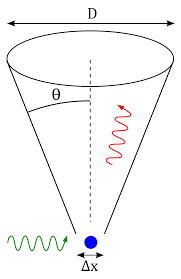
\includegraphics[width=3.5cm]{images/heisenberg_microscope.png}
\caption{Esperimento pensato del microscopio di Heisenberg.}\label{img-heisenberg_microscope}
\end{wrapfigure} 
\noindent A seconda dell'angolo di scattering dell'elettrone esso acquisirà un momento (più alta sarà l'energia del fotone più alto sarà il momento finale dell'elettrone).
Abbiamo quindi quella che viene chiamata \textbf{back action}: misurando un oggetto quantistico tramite un altro oggetto quantistico abbiamo influenzato e modificato il sistema stesso.
L'ottica classica ci fornisce una legge di diffrazione tale per cui:
\begin{equation*}
    \sin \theta \approx \frac{\lambda}{D}
\end{equation*}
Siccome il fotone è un'onda, il microscopio arriva a ottenere la posizione dell'elettrone con un'incertezza $\Delta x = \frac{\lambda}{\sin \theta}$ per cui si avrà:
\begin{equation*}
    -\frac{h}{\lambda}\sin \theta \le p_x \le \frac{h}{\lambda}\sin \theta
\end{equation*}
Da cui discende direttamente che: $\Delta p_x = \frac{2 h}{\lambda}\sin \theta$.
Dunque se voglio misurare solamente la posizione posso modificare $\lambda$ per avere una precisione arbitraria, ma non posso misurare in contemporanea il momento poiché:
\begin{equation*}
    \Delta p_x \Delta x = h
\end{equation*}
Che è una relazione evidentemente molto simile a quella ricavata dal principio di indeterminazione di Heisenberg: un'incertezza "alla Heisenberg" sulla sonda (il nostro fotone) ci porta a una necessaria incertezza sull'osservabile finale.
    %%%%%%%%%%%%%
% LECTURE 6 %
%%%%%%%%%%%%%

\vspace{1cm}

\noindent \lecture{6}{22/10/2021}

\section{Quantum Parallelism}

\begin{definizione}[\textbf{Quantum Parallelism}]
    Il \textbf{quantum parallelism} è una delle caratteristiche fondamentali di molti algoritmi quantistici. Consente ai computer quantistici di valutare una funzione $f(x)$ per molti valori diversi di $x$ contemporaneamente.
\end{definizione}
\noindent Supponiamo di considerare la più semplice funzione possibile $f(x):\{0,1\}^{\otimes n} \rightarrow \{0,1\}$ definita su un dominio (insieme di numeri costruiti con $n$ cifre di 0 e 1) e a elementi in un intervallo di bit. Assumiamo inoltre si saper calcolare efficientemente nel nostro computer tale funzione. Ciò che calcoliamo, dal punto di vista della computazione classica, lo possiamo valutare nella computazione quantistica, pertanto tutte le operazioni aritmetiche possono essere svolte dal calcolo quantistico. Un modo quindi di calcolare questa funzione su un computer quantistico è quello di considerare due differenti stati: immaginiamo un qubit $\ket{y}$ e uno stato che può essere un prodotto tensoriale di qubit, come ad esempio $\ket{0}^{\otimes n}$. Spesso considereremo lo stato $\ket{0}^{\otimes n}$ come stato iniziale in cui il computer quantistico viene preparato mediante una misurazione nella base computazionale perché è facilmente costruibile: ad esempio nel caso $n=3$ se, a seguito di una misurazione, lo stato nel QC collassa in $\ket{\psi} \rightarrow \ket{1} \otimes \ket{0} \otimes \ket{1}$, basterà applicare un \texttt{X-gate} al primo e al terzo qubit per costruire lo stato voluto $\ket{0}^{\otimes 3}$.

\noindent Chiamiamo lo stato iniziale totale $\ket{x,y}$, dove $x$ contiene l'informazione iniziale data in input e $y$ conterrà, dopo delle opportune operazioni, il risultato cercato. Con un'appropriata sequenza di gate è possibile effettuare la trasformazione
\begin{equation}\label{black_box_U_f}
    \ket{x,y} \overset{U_f}{\longrightarrow} \ket{x,y \oplus f(x)} \, ,
\end{equation}
dove $U_f$ è un opportuno gate unitario che implementa l'operazione desiderata. Il circuito che implementa la \eqref{black_box_U_f} è 
\begin{center}
    \mbox{
        \Qcircuit @C=1em @R=1em {
            \lstick{\ket{x}} & \multigate{1}{U_f} & \rstick{\ket{x}} \qw \\
            \lstick{\ket{y}} & \ghost{U_f} & \rstick{\ket{y\oplus f(x)}} \qw
        }
    }
\end{center}
dove $\ket{x}$ prende il nome di \textbf{data register} e $\ket{y}$ prende il nome di \textbf{target register}. Questa rappresentazione è utile perché quando $\ket{y} = \ket{0}$ l'output del target register è esattamente l'oggetto che si vuole calcolare
\begin{center}
    \mbox{
        \Qcircuit @C=1em @R=1em {
            \lstick{\ket{x}} & \multigate{1}{U_f} & \rstick{\ket{x}} \qw \\
            \lstick{\ket{0}} & \ghost{U_f} & \rstick{\ket{0\oplus f(x)}=\ket{f(x)}} \qw
        }
    }
\end{center}
Notiamo che la \eqref{black_box_U_f} è invertibile: se applichiamo $U_f$ due volte, otteniamo:
\begin{equation*}
    \ket{x,y} \rightarrow \ket{x, y \oplus f(x)} \rightarrow \ket{x,y \oplus f(x) \oplus f(x)} = \ket{x,y} \, ,
\end{equation*}
siccome $f(x) \oplus f(x) = 0$ indipendentemente dai valori di $f$. Fino ad ora avremmo potuto effettuare tutte queste operazioni in CC. L'importanza del QC risiede nel fatto che si possano considerare sovrapposizioni di stati appartenenti ad una base. Consideriamo il caso $n = 1$ (il data register è un qubit) e assumiamo il seguente stato iniziale
\begin{equation*}
    \ket{x,y} \equiv \underbrace{\frac{1}{\sqrt 2} (\ket{0}+\ket{1})}_{\ket{x}} \otimes \underbrace{\ket 0}_{\ket{y}} = \frac{1}{\sqrt 2} \left( \ket{00}+\ket{10} \right) \, ;
\end{equation*}
Se assumiamo che il computer sia preparato in $\ket{0} \otimes \ket{0}$ come possiamo rappresentare $\ket{x,y}$ in un circuito ? Possiamo sfruttare l'\texttt{H-gate} in questo modo:
\begin{center}
    \mbox{
        \Qcircuit @C=1em @R=1em {
            \lstick{\ket{0}} & \gate{H} & \multigate{1}{U_f} & \qw \\
            \lstick{\ket{0}} & \qw & \ghost{U_f} & \qw
            %\gategroup{1}{4}{2}{4}{0.8em}{\}}
        }
    }
\end{center}
infatti, utilizzando la \eqref{black_box_U_f}, avremo
\begin{equation*}
    \ket{0,0} \overset{H}{\longrightarrow} \frac{1}{\sqrt{2}} \left( \ket{00}+\ket{10} \right) \overset{U_f}{\longrightarrow} \frac{1}{\sqrt{2}} \left( \ket{0, f(0)} + \ket{1, f(1)} \right) \, .
\end{equation*}
Questo circuito è particolarmente interessante perché l'output è una sovrapposizione di differenti stati contenenti informazioni riguardo la funzione: $f(0)$ e $f(1)$ appaiono simultaneamente nel medesimo stato. È come se avessimo valutato $f(x)$ per due valori di $x$ contemporaneamente, parallelamente! A differenza del classic parallelism, in cui più circuiti vengono costruiti per calcolare $f(x)$ ed eseguiti simultaneamente, qui viene impiegato un singolo circuito per valutare la funzione $f(x)$ per più valori di $x$ nello stesso momento: si sta sfruttando la capacità di un computer quantistico di essere in sovrapposizioni di stati diversi. Qui risiede il \textbf{quantum parallelism}.

\noindent Questo discorso può essere facilmente generalizzato al caso di $n$-qubit. Supponiamo che il data register si trovi in $\ket{0}^{\otimes n}$. Usiamo il fatto che l'azione dell'\texttt{H-gate} su $n$-qubit possa essere scritta nel seguente modo:
\begin{align}
    H^{\otimes n}\ket{0}^{\otimes n} &= \underbrace{H\otimes \cdots \otimes H}_{n\text{-volte}} \underbrace{\ket{0} \otimes \cdots \otimes \ket{0}}_{n\text{-volte}} = \frac{1}{\sqrt 2} (\ket 0 + \ket 1) \otimes \cdots \otimes \frac{1}{\sqrt 2} (\ket 0 + \ket 1) \notag \\
    &= \frac{1}{\sqrt{2^n}}(\ket{000 \ldots 0} + \ket{010 \ldots 0} + \ldots + \ket{111 \dots 1}) = \frac{1}{\sqrt{2^n}}\sum_{x=0}^{2^n-1}\ket{x} \, , \label{n_H_gates}
\end{align}
dove $x$ rappresenta tutte le possibili stringhe di $n$-volte $0$ e $1$. Se il target si trova in $\ket{y} = \ket{0}$ e applichiamo ora $U_f$, il risultato è:
\begin{equation*}
    \frac{1}{\sqrt{2^n}}\sum_{x=0}^{2^n-1}\ket{x} \otimes \ket{0} \overset{U_f}{\longrightarrow} \frac{1}{\sqrt{2^n}}\sum_{x=0}^{2^n-1}\ket{x,f(x)} \, ,
\end{equation*}
dove si è fatto uso della \eqref{black_box_U_f} con $\ket{y} = \ket{0}$. In termini di circuiti avremo
\begin{center}
    \mbox{
        \Qcircuit @C=1em @R=1em {
            \lstick{\ket{0}^{\otimes n}} & \gate{H^{\otimes n}} & \multigate{1}{U_f} & \qw & \qw \\
            \lstick{\ket{y} = \ket{0}} & \qw & \ghost{U_f}   & \qw      & \qw
        }
    }
\end{center}
In un certo senso, il quantum parallelism consente di valutare simultaneamente tutti i possibili valori della funzione $f(x)$, anche se apparentemente abbiamo valutato $f(x)$ in una singola volta. Precisiamo che la misura dello stato nel caso del qubit singolo ci darà solamente $\ket{0, f(0)}$ oppure $\ket{1, f(1)}$. In maniera analoga per il caso generale, la misura dello stato $\sum_x\ket{x,f(x)}$ ci darà un solo $f(x_0)$ per un singolo valore casuale $x_0$. Ovviamente un computer classico può farlo più facilmente! La computazione quantistica richiede qualcosa di più del semplice quantum parallelism per essere utile; richiede cioè la capacità di estrarre informazioni su più di un valore di $f(x)$ da stati di sovrapposizione, come $\sum_x\ket{x,f(x)}$. Come vedremo nella prossima sezione, il "trucco" di considerare una sovrapposizione lineare ci permetterà di estrarre alcune informazioni su $f$ in un modo più efficiente del CC.

\section{Algoritmo di Deutsch}
Una semplice modifica del circuito precedente dimostra come i circuiti quantistici possano essere più performanti rispetto a quelli classici. Nelle ultime righe del paragrafo precedente abbiamo detto che la computazione quantistica richiede qualcosa di più oltre al quantum parallelism per essere utilizzabile. L'\textbf{algoritmo di Deutsch} combina il meccanismo del \textbf{quantum parallelism} con la proprietà della meccanica quantistica dell'\textbf{interferenza}. 

\noindent Si tratta di un algoritmo un po' accademico (le funzioni sono banali), tuttavia utile per illustrare l'idea di algoritmo quantistico. Lasciamo che entrambi input e output register contengano ciascuno un solo qubit, quindi stiamo esplorando le funzioni $f(x)$ che convertono un singolo bit in un singolo bit: $f(x): \; \{ 0,1 \} \rightarrow \{ 0,1 \}$. Ci sono due modi piuttosto diversi di pensare a tali funzioni. Il primo modo è notare che ci sono solo quattro di queste funzioni, come mostrato nella Tabella \ref{tab:Deutsch_Fnct}.

\begin{table}[!ht]
	\centering
    \begin{tabular}{ccc}
        \toprule
        & $x = 0$ & $x=1$ \\
        \midrule
        $f_0$ & $0$ & $0$ \\
        $f_1$ & $0$ & $1$ \\
        $f_2$ & $1$ & $0$ \\
        $f_3$ & $1$ & $1$ \\
        \bottomrule
    \end{tabular} \\
    \caption{Esistono solo quattro funzioni distinte $f_j(x)$ che convertono un bit in un bit, tutte facilmente implementabili sia in un computer classico che quantistico.}
    \label{tab:Deutsch_Fnct}
\end{table}

\noindent Supponiamo che ci venga data una black-box (ossia un gate ignoto che indicheremo con \texttt{U-gate}) che calcola una di queste quattro funzioni eseguendo la seguente trasformazione unitaria:
\begin{equation*}
    U_{f_j} \ket{x,y} = \ket{x, y \oplus f_j(x)} \, .
\end{equation*}
In questo caso, se implementiamo in circuiti la Tabella \ref{tab:Deutsch_Fnct} avremo:

\begin{center}
    \mbox{
        $
        \begin{matrix}
             \\
             \\
            f_0: \\
        \end{matrix}
        $
        \Qcircuit @C=1em @R=1em {
            & \multigate{1}{U_{f_0}} & \qw \\
            & \ghost{U_{f_0}}& \qw \\
        }
        $
        \begin{matrix}
             \\
             \\
            \ = \\
        \end{matrix}
        $
        \Qcircuit @C=1em @R=1.9em {
            & \qw & \qw & \qw & \qw & \qw \\
            & \qw & \qw & \qw & \qw & \qw \\
        }
    }
    \qquad \qquad
    \mbox{
        $
        \begin{matrix}
             \\
             \\
            f_1: \\
        \end{matrix}
        $
        \Qcircuit @C=1em @R=1em {
            & \multigate{1}{U_{f_1}} & \qw \\
            & \ghost{U_{f_1}}& \qw \\
        }
        $
        \begin{matrix}
             \\
             \\
            \ = \\
        \end{matrix}
        $
        \Qcircuit @C=1em @R=1.35em {
            & \ctrl{1} & \qw & \qw \\
            & \targ & \qw & \qw  \\
        }
    }
\end{center}
\begin{center}
    \mbox{
        $
        \begin{matrix}
             \\
             \\
            f_2: \\
        \end{matrix}
        $
        \Qcircuit @C=1em @R=1em {
            & \multigate{1}{U_{f_2}} & \qw \\
            & \ghost{U_{f_2}}& \qw \\
        }
        $
        \begin{matrix}
             \\
             \\
            \ = \\
        \end{matrix}
        $
        \Qcircuit @C=1em @R=1.15em {
            & \qw & \ctrl{1} & \qw \\
            & \gate{X} & \targ & \qw \\
        }
    }
    \qquad \qquad
    \mbox{
        $
        \begin{matrix}
             \\
             \\
            f_3: \\
        \end{matrix}
        $
        \Qcircuit @C=1em @R=1em {
            & \multigate{1}{U_{f_3}} & \qw \\
            & \ghost{U_{f_3}}& \qw \\
        }
        $
        \begin{matrix}
             \\
             \\
            \ = \\
        \end{matrix}
        $
        \Qcircuit @C=1em @R=1.25em {
            & \qw & \qw \\
            & \gate{X} & \qw \\
        }
    }
\end{center}
Dato che la regola che vogliamo implementare è $\ket{x,0} \rightarrow \ket{x, f(x)}$ ($\ket{y}$ inizializzato a $\ket{0}$), in termini matematici questo significa scrivere:
\begin{align*}
    &f_0: &\ket{x,0} &\longrightarrow \ket{x,0} \, , \\
    &f_1: &\ket{x,0} &\overset{\texttt{CNOT}}{\longrightarrow} 
    \begin{cases}
        \ket{0,0} \, , &\text{per } x = 0 \\
        \ket{1,1} \, , &\text{per } x = 1
    \end{cases} \, , \\
    &f_2: &\ket{x,0} &\overset{X}{\longrightarrow} \ket{x,1} \overset{\texttt{CNOT}}{\longrightarrow}
    \begin{cases}
        \ket{0,1} \, , &\text{per } x = 0 \\
        \ket{1,0} \, , &\text{per } x = 1
    \end{cases} \, , \\
    &f_3: &\ket{x,0} &\overset{X}{\longrightarrow} \ket{x,1} \, , 
\end{align*}

\noindent Supponiamo che ci venga data una black-box che esegua $U_f$ per una delle quattro funzioni, ma non ci venga detto quale delle quattro operazioni. Ovviamente possiamo scoprirlo lasciando agire due volte la black-box, prima su $\ket0 \otimes \ket0$ e poi su $\ket 1 \otimes \ket 0$. Ma supponiamo di poter far agire la black-box solo una volta. Cosa possiamo conoscere di $f(x)$ ?

\noindent In un computer classico, dove siamo effettivamente limitati a lasciare che la black-box agisca sui qubit in uno dei quattro stati di base computazionale, possiamo conoscere il valore di:
\begin{itemize}
    \item $f(0)$, lasciando che $U_f$ agisca su uno dei due $\ket0 \otimes \ket0$ o $\ket0 \otimes \ket1$;
    \begin{itemize}
        \item In tal caso possiamo limitare la scelta a $f_0$ o $f_1$ (se $f(0) = 0$) oppure $f_2$ o $f_3$ (se $f(0) = 1$).
    \end{itemize}
    \item $f(1)$, lasciando che $U_f$ agisca su $\ket1 \otimes \ket0$ o $\ket1 \otimes \ket1$;
    \begin{itemize}
        \item In questa situazione abbiamo ristretto la funzione ad essere $f_0$ o $f_2$ (se $f(1) = 0$) oppure $f_1$ o $f_3$ (se $f(1) = 1$).
    \end{itemize}
\end{itemize}
In definitiva, un computer classico necessita di due esecuzioni per determinare se $f$ sia costante o meno. Sorprendentemente, risulta che con un computer quantistico questo non è necessario perché il problema può essere risolto con una singola esecuzione. Il punto interessante è che l'algoritmo non riguarda il calcolo preciso della funzione, ma piuttosto la comprensione di una o più sue proprietà: quando l'algoritmo viene lanciato non impariamo nulla sui valori individuali di $f(0)$ e $f(1)$, ma siamo comunque in grado di rispondere alla domanda sui loro valori relativi. Chiaramente otteniamo meno informazioni di quelle che otterremmo rispondendo alla domanda con un computer classico, ma, rinunciando alla possibilità di acquisire quella parte dell'informazione che è irrilevante per la domanda a cui vogliamo rispondere, possiamo ottenere la risposta con una sola applicazione di $U_f$.

\noindent Come sottolineato in precedenza l'algoritmo combina il quantum parallelism e l'interferenza: possiamo preparare il computer nello stato $\ket 0 \otimes \ket 1$ della base canonica e applicare l'\texttt{H-gate} a entrambi i qubit: 
\begin{equation}\label{eq:Deutsch_1}
    (H\otimes H) \ket{0} \otimes \ket{1} = \underbrace{\frac{\ket0 + \ket1}{\sqrt 2}}_{\substack{\text{quantum} \\ \text{parallelism}}} \otimes \underbrace{\frac{\ket0-\ket1}{\sqrt 2}}_{\text{interferenza}} \, ;
\end{equation}
in un circuito significa scrivere
\begin{center}
    \mbox{
        \Qcircuit @C=1em @R=1em {
            \lstick{\ket{0}} & \gate{H} & \multigate{1}{U_f} & \qw \\
            \lstick{\ket{1}} & \gate{H} & \ghost{U_f} & \qw
        }
    }
\end{center}
Chiamando per semplicità $\ket{x} \equiv \frac{1}{\sqrt{2}} (\ket{0} + \ket{1})$ e applicando $U_f$ alla \eqref{eq:Deutsch_1} tramite \eqref{black_box_U_f}, possiamo esplicitamente vedere che cosa implica il termine di interferenza:
\begin{align*}
    &\ket{x} \otimes \frac{1}{\sqrt 2} (\ket 0 - \ket 1) \overset{U_f}{\longrightarrow} \frac{1}{\sqrt 2} \left( \ket{x, 0 \oplus f(x)} - \ket{x, 1 \oplus f(x)} \right) \\
    &=
    \begin{cases}
        \frac{1}{\sqrt 2} \left( \ket{x, 0 \oplus 0} - \ket{x, 1 \oplus 0} \right) = \ket x \otimes \frac{1}{\sqrt 2} (\ket 0 - \ket 1) \, , \quad &\text{per } f(x) = 0 \\
        \frac{1}{\sqrt 2} \left( \ket{x, 0 \oplus 1} - \ket{x, 1 \oplus 1} \right) = - \ket x \otimes \frac{1}{\sqrt 2} (\ket 0 - \ket 1) \, , \quad &\text{per } f(x) = 1
    \end{cases} \, .
\end{align*}
Combinando i due casi in un'unica espressione compatta abbiamo ottenuto
\begin{equation}\label{black_box_action_U_f_on_x}
    \ket{x} \otimes \frac{1}{\sqrt 2} (\ket 0 - \ket 1) \overset{U_f}{\longrightarrow} (-1)^{f(x)} \ket x \otimes \frac{1}{\sqrt 2} (\ket 0 - \ket 1) \, ,
\end{equation}
Sostituendo $\ket{x}$ con lo stato iniziale che implementava il quantum parallelism avremo
\begin{equation*}
    \frac{\ket{0} + \ket{1}}{\sqrt{2}} \otimes \frac{\ket 0 - \ket 1}{\sqrt 2} \overset{U_f}{\longrightarrow} \frac{1}{\sqrt{2}} \left[ (-1)^{f(0)} \ket 0 + (-1)^{f(1)} \ket 1 \right] \otimes \frac{\ket 0 - \ket 1}{\sqrt 2} \, ;
\end{equation*}
dato che il segno relativo nella parentesi quadra dipende dal fatto che $f(0)$ e $f(1)$ siano uguali o meno, possiamo riscrivere quest'ultima espressione come
\begin{equation*}
    \begin{cases}
        (-1)^{f(0)}\frac{\ket 0 + \ket 1}{\sqrt 2}\otimes\frac{\ket 0-\ket 1}{\sqrt 2} \, , &\text{per }f(0) = f(1) \\
        (-1)^{f(0)}\frac{\ket 0 - \ket 1}{\sqrt 2}\otimes\frac{\ket 0-\ket 1}{\sqrt 2} \, , &\text{per }f(0) \neq f(1) 
    \end{cases} \, .
\end{equation*}
Come ultimo passaggio si applica l'\texttt{H-gate} al primo qubit in maniera tale che il circuito totale diventi:
\begin{center}
    \mbox{
        \Qcircuit @C=1em @R=1em {
            \lstick{\ket{0}} & \gate{H} & \multigate{1}{U_f} & \gate{H} & \qw \\
            \lstick{\ket{1}} & \gate{H} & \ghost{U_f} & \qw & \qw
        }
    }
\end{center}
Questa modifica trasforma il risultato precedente in 
\begin{equation*}
    \begin{cases}
        (-1)^{f(0)}\frac{\ket 0 + \ket 1}{\sqrt 2}\otimes\frac{\ket 0-\ket 1}{\sqrt 2} \overset{H}{\longrightarrow} (-1)^{f(0)}\ket 0\otimes\frac{\ket 0-\ket 1}{\sqrt 2} \, , &\text{per }f(0) = f(1) \\
        (-1)^{f(0)}\frac{\ket 0 - \ket 1}{\sqrt 2}\otimes\frac{\ket 0-\ket 1}{\sqrt 2} \overset{H}{\longrightarrow} (-1)^{f(0)}\ket 1\otimes\frac{\ket 0-\ket 1}{\sqrt 2} \, , &\text{per }f(0) \neq f(1) 
    \end{cases} \, .
\end{equation*}
Il risultato finale ci suggerisce che possiamo effettuare solamente una misurazione sul primo qubit: ottenendo $\ket{0}$ o $\ket{1}$ siamo in grado, con una singola misura, di stabilire se $f(0) = f(1)$ oppure $f(0) \neq f(1)$. Questo significa che siamo in grado di escludere 2 delle 4 funzioni con una singola esecuzione dell'algoritmo. 

\noindent Questo esempio permette di evidenziare quale sia la differenza tra il quantum parallelism e gli algoritmi randomizzati classici. Ingenuamente, si potrebbe pensare che lo stato finale corrisponda piuttosto a un calcolatore classico probabilistico che valuta $f(0)$ con probabilità $\frac 12$, o $f(1)$ con probabilità $\frac 12$. La differenza è che in un computer classico queste due alternative si escludono sempre mentre in un computer quantistico è possibile che le due alternative interferiscano l'una con l'altra per ottenere alcune proprietà globali della funzione $f(x)$. Utilizzando un opportuno gate (nel nostro caso l'\texttt{H-gate}) siamo in grado di ricombinare le diverse alternative.

\section{Algoritmo di Deutsch-Jozsa}
L'algoritmo di Deutsch è un semplice caso di un algoritmo quantistico più generale, noto come \textbf{algoritmo di Deutsch-Jozsa}, che evidenzia esplicitamente come il QC offra un grosso miglioramento rispetto ai metodi del CC. Supponiamo di avere una black-box che calcola una funzione booleana $f(x): \; \{0,1\}^{\otimes n}\rightarrow \{0,1\}$ e supponiamo di sapere per certo che $f(x)$ sia solamente una delle seguenti alternative:
\begin{itemize}
    \item \textbf{Funzione costante} (\textit{constant}): l'output è sempre $0$ oppure $1$ indipendentemente dall'input.
    \item \textbf{Funnzione bilanciata} (\textit{balanced}): l'output è costituito per metà dal valore $0$ e metà dal valore $1$.
\end{itemize}
Lo scopo dell'algoritmo è quello di capire quale delle due sia l'alternativa corretta con il minor numero di esecuzioni. Classicamente potremmo risolvere questo problema calcolando $2^{n-1}+1$ valori della funzione perché è necessario calcolare almeno una metà dei valori più un valore aggiuntivo. Chiaramente si tratta di un numero esponenzialmente grande. Quello che fa l'algoritmo di Deutsch-Jozsa è risolvere il problema perfettamente con una sola query quantistica. Cominciamo scrivendo il circuito che descrive tale algoritmo, il quale è molto simile a quello di Deutsch con la sola differenza che il data register non è un singolo qubit, ma piuttosto un prodotto tensoriale di $n$-qubit:
\begin{center}
    \mbox{
        \Qcircuit @C=1em @R=1em {
            \lstick{\ket{0}^{\otimes n}} & \gate{H^{\otimes n}} & \multigate{1}{U_f} & \gate{H^{\otimes n}} & \qw \\
            \lstick{\ket{1}} & \gate{H} & \ghost{U_f} & \qw & \qw
        }
    }
\end{center}
Vediamo nello specifico cosa succede all'interno del circuito:
\begin{enumerate}
    \item Viene inizializzato (preparato) lo stato in $\ket{0}^{\otimes n} \otimes \ket{1}$;
    \item Creiamo una sovrapposizione di stati usando l'\texttt{H-gate} su tutti gli $n+1$ qubit:
        \begin{equation*}
            \ket{0}^{\otimes n} \otimes \ket{1} \overset{H}{\longrightarrow} \frac{1}{\sqrt {2^n}}\sum_{x=0}^{2^n-1}\ket x \otimes \frac{\ket 0 - \ket 1}{\sqrt 2} \, ,
        \end{equation*}
        dove si è fatto uso della \eqref{n_H_gates}. Notiamo che ora nell'output register è presente lo stato che nella sezione precedente avevamo visto essere associato all'interferenza. 
    \item Valutiamo la funzione $f(x)$ usando la block-box di $U_f$
        \begin{equation*}
            \frac{1}{\sqrt {2^n}}\sum_{x=0}^{2^n-1}\ket x \otimes \frac{\ket 0 - \ket 1}{\sqrt 2} \overset{U_f}{\longrightarrow} \sum_{x=0}^{2^n-1}\frac{(-1)^{f(x)}}{\sqrt{2^n}}\ket x \otimes \frac{\ket 0 - \ket 1}{\sqrt 2} \, ,
        \end{equation*}
        dove, essendo $\ket{x}$ arbitrario, abbiamo fatto uso della \eqref{black_box_action_U_f_on_x}. 
    \item Applichiamo nuovamente l'\texttt{H-gate} ai primi $n$ qubit. Per capire il risultato di $H^{\otimes n} \ket{x}$ consideriamo per semplicità il caso $n=1$: formalmente avremo 
    \begin{equation*}
        H \ket{x} = \sum_{z = 0}^1 \frac{(-1)^{xz}}{\sqrt{2}} \ket{z} \, , \; \text{ dove } x = 0 \text{ oppure } 1 \, .
    \end{equation*}
    Per $n$ generico possiamo generalizzare scrivendo
    \begin{align*}
        H^{\otimes n} \ket{x} &= (H \otimes \ldots \otimes H) \ket{x_0} \otimes \ket{x_1} \otimes \ldots \otimes \ket{x_{n-1}} \\
        &= \sum_{z_0=0}^1 \ldots \sum_{z_{n-1}=0}^1 \frac{(-1)^{x_0 z_0} (-1)^{x_1 z_1} \cdots (-1)^{x_{n-1} z_{n-1}}}{\sqrt{2^n}} \ket{z} \, ,
    \end{align*}
    dove $\ket{z} \equiv \ket{z_0, z_1, \ldots, z_{n-1}}$. In maniera più compatta possiamo scrivere quindi l'azione dell'\texttt{H-gate} sugli $n$ qubit (nonché risultato finale del circuito) come
        \begin{equation}\label{output_Deutsch_Jozsa}
            \sum_{z = 0}^{2^n-1} \sum_{x = 0}^{2^n-1} \frac{(-1)^{f(x) + x \cdot z}}{2^n}\ket z \otimes \frac{\ket 0 - \ket 1}{\sqrt 2} \, ,
        \end{equation}
        dove abbiamo indicato con $x\cdot z$ il \textbf{prodotto bit a bit modulo 2}:
        \begin{equation*}
            x\cdot z = (x_0z_0 + \ldots + x_{n-1}z_{n-1}) \mod{2} \, .
        \end{equation*}
    \item Infine misuriamo per ottenere lo stato finale $\ket{z}$. 
\end{enumerate}

\noindent Ricordiamo che il problema è quello di determinare se $f$ sia constant o balanced. Notiamo dal risultato \eqref{output_Deutsch_Jozsa} che il data register ora contiene una sovrapposizione lineare di tutti i possibili stati che si scrivono come stringhe contenenti $n$ volte 0 e 1. In $\ket{z}$ è presente un caso particolare: consideriamo la situazione in cui $\ket z = \ket{00\ldots0} = \ket0^{\otimes n}$ e cerchiamo la probabilità di ottenere tale stato guardando il modulo quadro del coefficiente:
\begin{equation*}
    P \left( \ket{z} = \ket0^{\otimes n} \right) = \abs{\sum_{x=0}^{2^n-1}\frac{(-1)^{f(x)}}{2^n}}^2 = 
    \begin{cases}
    1 \, , &\text{se } f(x) \text{ è constant} \\
    0 \, , &\text{se } f(x) \text{ è balanced} 
    \end{cases} \, .
\end{equation*}
Notiamo che quando la probabilità è 1 a numeratore si hanno $2^n$ termini tutti uguali ($(-1)^1$ oppure $(-1)^0$) che si semplificano con il fattore $1/2^n$; quando invece la probabilità è nulla a numeratore si ha uno stesso numero di $(-1)^1$ e $(-1)^0$ che si cancellano esattamente. Come abbiamo detto $\ket z=\ket0^{\otimes n}$ è un caso particolare molto importante perché permette di risolvere il problema mediante la misura dello stato. Se misurando $z$ otteniamo $\ket{0}^{\otimes n}$ allora, con probabilità 1 (quindi sempre), lo stato è $\ket{0}^{\otimes n}$ e la funzione è constant; al contrario quando la misura di $z$ produce un qualsiasi stato differente da $\ket{0}^{\otimes n}$ allora, essendo $P \left( \ket{z} = \ket0^{\otimes n} \right) = 0$, lo stato $\ket{0}^{\otimes n}$ non è nemmeno presente in $z$ e possiamo stabilire con assoluta certezza che la funzione è balanced. Il fatto importante è che essendo queste misure mutualmente esclusive, possiamo determinare se $f$ sia constant o balanced con una singola misurazione. Quindi si tratta di effettuare una sola misurazione in QC contro $\mathcal{O}(2^n)$ misure in CC.

\noindent Osserviamo che il confronto tra algoritmi classici e quantistici è in qualche modo un confronto delicato, poiché il metodo per valutare la funzione è abbastanza diverso nei due casi. Se fosse consentito utilizzare un computer probabilistico classico, per valutare $f(x)$ per pochi $x$ scelti a caso, si può determinare molto rapidamente con alta probabilità se $f(x)$ è \textit{constant} o \textit{balanced}. Questo scenario probabilistico è forse più realistico dello scenario deterministico che abbiamo considerato.

\noindent Ribadiamo nuovamente che questo algoritmo è un esempio molto accademico in quanto non esistono problemi fisici o matematici reali che necessitano di sapere se una funzione sia constant o balanced. Nonostante ciò il fatto importante è che grazie a questo algoritmo quantistico non è più necessario aspettare un tempo esponenzialmente\footnote{Talvolta non si vuole sapere con precisione assoluta se $f$ sia constant o balanced, ma è sufficiente stabilirlo entro un errore dato $\varepsilon$. Un ipotetico algoritmo classico e probabilistico di questo tipo diventa di ordine polinomiale in $n$: passare da $\mathcal{O}(\text{polinomio in }n)$ a $\mathcal{O}(1)$ mediante la controparte quantistica non è più un miglioramento così estremo come passare da $\mathcal{O}(2^n)$ ad $\mathcal{O}(1)$ !} crescente nel numero di bit per sapere il risultato. 

\section{Algoritmo di Bernstein-Vazirani}
Consideriamo un altro algoritmo di black-box per il quale gli algoritmi quantistici forniscono un vantaggio: l'\textbf{algoritmo di Bernstein-Vazirani}. Qui, a differenza dei due casi precedenti, abbiamo accesso alla funzione della black-box $f: \{0, 1\}^n \rightarrow \{0, 1\}$. Supponiamo che la funzioni sia data da\footnote{Come prima il simbolo "$\cdot"$ indica il prodotto bit a bit modulo 2}:
\begin{equation*}
    f(x) = a\cdot x = (a_0 x_0 + \ldots + a_{n-1} x_{n-1})\mod{2} \, , \; \text{ dove } a \geqslant 0 \text{ e } x < 2^n \, .
\end{equation*}
Sappiamo che la funzione è lineare, tuttavia l'obiettivo di questo algoritmo è trovare il valore di $a$. Classicamente, questo problema potrebbe richiedere $n$ query poiché ogni query può fornire solo un nuovo bit di informazioni su $a$, ma $a$ possiede $n$ bit: dobbiamo valutare $f(1000\ldots) = a_0$, $f(0100\ldots) = a_1$ e così via con $n$ valutazioni fino a $f(111\ldots1) = a_{n-1}$. L'algoritmo di Bernstein-Vazirani, invece, risolve il problema quantisticamente utilizzando una sola query!

\noindent Consideriamo il medesimo circuito dell'algoritmo di Deutsch-Josza e il suo output \eqref{output_Deutsch_Jozsa}: nel caso in cui $f(x) = a \cdot x$ esso diventa 
\begin{equation*}
    \sum_{z=0}^{2^n-1}\sum_{x=0}^{2^n-1}\frac{(-1)^{x\cdot (a+z)}}{2^n}\ket z \otimes \frac{\ket 0 - \ket 1}{\sqrt 2} \, .
\end{equation*}
Come nell'algoritmo precedente guardiamo il coefficiente di $\ket{z}$:
\begin{equation*}
        \frac{1}{2^n} \sum_{x=0}^{2^n-1}(-1)^{x\cdot (a+z)} = (-1)^{x_0(a_0+z_0) + \ldots + x_{n-1}(a_{n-1}+z_{n-1})} = \frac{1}{2^n} \prod_{j=0}^{n-1} \left( \sum_{x_j=0}^{1}(-1)^{x_j(a_j+z_j)} \right) \, ,
\end{equation*}
ma ogni termine nella parentesi tonda è la somma di termini che possono essere $\pm 1$ a seconda dell'esponente. Distinguiamo i due casi:
\begin{itemize}
    \item Se $(a_j+z_j=0)\mod2 $ allora il coefficiente è 
    \begin{equation*}
        \frac{1}{2^n} \prod_{j=0}^{n-1}(2) = 1 \, , \quad \Rightarrow \quad \text{Probabilità } 1 \, .
    \end{equation*}
    \item Al contrario quando $(a_j+z_j=1)\mod2$ allora il coefficiente diventa 
    \begin{equation*}
        \frac{1}{2^n} \prod_{j=0}^{n-1} \left[ (-1)^{0\cdot 1} + (-1)^{1 \cdot 1} \right] = 0 \, , \quad \Rightarrow \quad \text{Probabilità } 0 \, .
    \end{equation*}
\end{itemize}
Ancora una volta, i due casi della probabilità sono mutualmente esclusivi e quindi avremo
\begin{align*}
    &(a_j+z_j=0)\mod2 \, , \quad \Rightarrow \quad a = z \, , \quad \Rightarrow \quad \text{Probabilità } 1 \, , \\
    &(a_j+z_j=1)\mod2 \, , \quad \Rightarrow \quad a \neq z \, , \quad \Rightarrow \quad \text{Probabilità } 0 \, .
\end{align*}
Questo significa che il nostro stato, in realtà, non è una sovrapposizione lineare, ma contiene bensì solamente lo stato
\begin{equation*}
    \ket a \otimes \frac{\ket 0 - \ket 1}{\sqrt 2} \, ;
\end{equation*}
e quindi attraverso un'unica operazione di misura sui primi $n$-qubit, otteniamo $a$, la nostra incognita.
    %%%%%%%%%%%%%
% LECTURE 7 %
%%%%%%%%%%%%%

\vspace{1cm}

\noindent\lecture{7}{25/10/2021}
\vspace{0.5cm}
\noindent I prossimi due algoritmi sono tra quelli più conosciuti, in termini di algoritmi quantistici, sia dal punto di vista storico del QC sia dal punto di vista applicativo:
\begin{itemize}
    \item L'algoritmo di ricerca del periodo di una funzione: l'\textbf{algoritmo di Shor};
    \item L'algoritmo di ricerca di particolari elementi in un database: l'\textbf{algoritmo di Grover}.
\end{itemize}
Prima di addentrarci nello studio del più difficile (non vedremo tutto il discorso legato alla teoria dei numeri) dei due, l'algoritmo di Shor, introduciamo il seguente concetto:


\section{Quantum Fourier Transform}
Il cuore dell'algoritmo di Shor è la \textbf{QFT} o \textbf{Quantum Fourier Transform}, che può essere eseguita da un circuito quantistico. La QFT di $n$ qubit è definita come quella trasformazione unitaria $\hat U_{\text{FT}}$ la cui azione su un elemento $\ket{x} \in \mathcal{H}$ è data da:
\begin{equation}\label{QFT}
    \hat U_{\text{FT}}\ket x = \frac{1}{2^{\frac n2}}\sum_{y=0}^{2^n-1}e^{2\pi i\frac{ x \cdot y }{2^n}}\ket y
\end{equation}
dove con la notazione precedente intendiamo $\ket{x} \equiv \ket{x_{n-1}} \otimes \ket{x_{n-2}} \otimes \ldots \otimes \ket{x_0}$, in cui ciascun qubit $\ket{x_i}$ può essere un elemento della base computazionale, quindi $\ket{0}$ o $\ket{1}$. Notiamo inoltre che il prodotto $x \cdot y$ ad esponente è un prodotto scalare tra interi e non un prodotto bit a bit modulo 2. Lo stato $\ket{x}$ può essere scritto utilizzando anche la codifica digitale degli interi, ossia
\begin{equation*}
    x = 2^{n-1} x_{n-1} + 2^{n-2} x_{n-2} + \ldots + 2^{0} x_0 \, , \; \text{ dove } 0 \leqslant x \leqslant 2^n - 1 \, .
\end{equation*}
Notiamo che il fattore davanti alla sommatoria in \eqref{QFT} è un fattore di normalizzazione perchè abbiamo diviso per la radice del numero totale degli stati: lo spazio di Hilbert di $\ket{x}$ ha infatti $\dim \mathcal{H} = 2^n$ poiché è frutto del prodotto tensoriale degli $n$ spazi associati ai singoli qubit. Dato che $\hat U_{\text{FT}}$ è un operatore che agisce su $\mathcal{H}$, possiamo applicare la \eqref{QFT} ad una sovrapposizione di stati $\ket x$ con ampiezze complesse $\gamma(x)$:
\begin{equation}
    \label{eq:qtf2}
    \hat U_{\text{FT}} \left( \sum_{x=0}^{2^n-1}\gamma(x)\ket x \right) = \sum_{x,y=0}^{2^n-1} \frac{\gamma(x)}{2^{\frac n2}} e^{2\pi i \frac{x\cdot y}{2^n}} \ket y = \sum_{y=0}^{2^n-1}\hat \gamma(y)\ket y \, ,
\end{equation}
dove abbiamo ottenuto un'altra sovrapposizione con ampiezze che sono legate a $\gamma(x)$ dalla \textbf{DFT} o \textbf{Discrete Fourier Transform}:
\begin{equation}\label{DFT}
    \hat \gamma(y)=\sum_{x=0}^{2^n-1}\frac{e^{2\pi i \frac{x\cdot y}{2^n}}}{2^{\frac n2}}\gamma(x) \, .
\end{equation}
Si noti che la \eqref{QFT} agisce sui coefficienti $\gamma(x)$ come in \eqref{DFT}, ossia tramite una versione discretizzata della trasformata di Fourier standard. In generale la DFT è largamente utilizzata nella teoria dei segnali. 

\noindent Per calcolare ciascun coefficiente $\hat{\gamma}(x)$ in \eqref{DFT} si richiedono $2^n \times 2^n = 2^{2n}$ operazioni (dimensione della matrice), le quali sono un enormità ! In CC esiste un celebre algoritmo chiamato \textbf{FFT} o \textbf{Fast Fourier Transform} che migliora il numero precedente fino a $\order{n 2^n}$, ottenendo quindi un modo molto più efficiente per calcolare $\hat{\gamma}(x)$. In realtà esiste un algoritmo quantistico per eseguire la trasformazione unitaria $\hat U_{\text{FT}}$ in un tempo esponenzialmente più veloce, perché cresce solo come $\order{n^2}$. Il problema, come al solito, è che non si può conoscere l'insieme completo dei coefficienti di Fourier, come si fa dopo aver applicato la FFT: il risultato è infatti una sovrapposizione $\sum_y \hat{\gamma} (y) \ket{y}$ sulla quale è necessario effettuare una misurazione che permetterà di ottenere solamente 1 coefficiente. Nonostante quindi l'algoritmo per il calcolo della QFT non migliori l'algoritmo classico della FFT, la \eqref{QFT} si è rivelata molto utile per la risoluzione di problemi del mondo quantistico. Ad esempio, se $\gamma$ è una funzione periodica con un periodo $r$ non maggiore di $2^{\frac n2}$, allora un registro nello stato \eqref{eq:qtf2} può fornire potenti indizi sul valore preciso del periodo, anche se $r$ può essere lungo centinaia di cifre. Per il momento il nostro scopo è mostrare che è possibile costruire un circuito che calcoli in un numero di step di ordine $\order{n^2}$ la QFT.

\noindent Consideriamo, come al solito, come punto di partenza lo stato $\ket 0^{\otimes n}$. Sappiamo dalla \eqref{n_H_gates} che se applichiamo l'\texttt{H-gate} su tale stato avremo
\begin{equation*}
    H^{\otimes n}\ket{0}^{\otimes n} = \frac{1}{2^{\frac n2}}\sum_{y=0}^{2^n-1} \ket y \, ,
\end{equation*}
ossia una somma su tutti gli stati nella base computazionale. Definiamo ora un operatore $\mathcal{Z}$ che agisce nel modo seguente:
\begin{equation*}
    \mathcal{Z}\ket y = e^{2\pi i \frac{y}{2^n}}\ket y \, ;
\end{equation*}
in questo modo l'operatore $\hat U_{\text{FT}}$ della \eqref{QFT} può essere riscritto come
\begin{equation}\label{QFT_with_Z}
    \hat U_{\text{FT}}\ket x = \mathcal{Z}^xH^{\otimes n}\ket{0}^{\otimes n} = \frac{1}{2^{\frac n2}}\sum_{y=0}^{2^n-1} \mathcal{Z}^x \ket y \, , \; \text{ con } \mathcal{Z} = e^{2\pi i \frac{xy}{2^n}} \, ;
\end{equation}
si ricordi sempre che $x$ è un intero. Cerchiamo di capire cosa sia $\mathcal Z$. Consideriamo il caso del qubit singolo ($n=1$):
\begin{equation*}
    \mathcal{Z}\ket y = e^{\pi i y}\ket{y} = 
    \begin{cases}
        \ket{y} \, , &\text{per } y = 0 \\
        -\ket{y} \, , &\text{per } y = 1
    \end{cases}
    \, , \quad \Rightarrow \quad \mathcal{Z} = Z = 
    \begin{pmatrix}
        1 & 0 \\ 0 & -1
    \end{pmatrix} \, .
\end{equation*}
Si noti che un altro modo conveniente di scriverlo è come esponenziale
\begin{equation*}
    Z = e^{i \pi n} \, , \; \text{ dove } n = 
    \begin{pmatrix}
        0 & 0 \\ 0 & 1
    \end{pmatrix} \, .
\end{equation*}
Per passare alla generalizzazione per $n$ qubit ricordiamo che, come lo stato $\ket{x}$ di \eqref{QFT}, possiamo scrivere nella base computazionale che $ \ket y = \ket{y_{n-1}} \otimes \ldots \otimes \ket{y_0}$ e analogamente come intero avremo $y = 2^{n-1} y_{n-1} + \ldots + 2^0 y_0$. Introduciamo $n$ differenti matrici, che chiameremo $n_i$ con $i = 0, \ldots, n-1$, che agiscono sul corrispondente qubit di $\ket{y}$ dando 0 o 1 a seconda del valore del qubit: questo significa scrivere che
\begin{equation*}
    \left( 2^{n-1} n_{n-1} + 2^{n-2} n_{n-2} + \ldots + n_0 \right) \ket y = 2^{n-1} y_{n-1} \ket{y_{n-1}} \otimes \ldots \otimes 2^0 y_0 \ket{y_0} = y\ket y \, ,
\end{equation*}
quindi si tratta di un particolare modo di calcolare la codifica digitale, ossia l'intero $y$, dello stato $\ket{y}$. Notiamo che la matrice $n_{n-1}$ agisce su $\ket{y_{n-1}}$, $n_{n-2}$ agisce su $\ket{y_{n-2}}$ e così via fino a $n_0$ che agisce su $\ket{y_0}$,   questo perché in generale $n_p \ket{y_p} = y_p \ket{y_p}$. Utilizzando quindi questa notazione possiamo riscrivere l'operatore $\mathcal{Z}$ in questo modo: 
\begin{equation*}
    \mathcal{Z} \ket y = e^{\frac{2 \pi i}{2^n} y} \ket y = e^{\frac{2\pi i}{2^n} (2^{n-1}n_{n-1}+\dots+n_0)} \ket y \, ,
\end{equation*}
dove si è utilizzata la formula $n_p \ket{y_p} = y_p \ket{y_p}$ ad esponente e si è riconosciuta la codifica digitale di $y$. Per calcolare la QFT come in \eqref{QFT_with_Z} ci serve saper calcolare $\mathcal{Z}^x$. Al posto che farlo in generale, focalizziamoci su un esempio perché vedremo alla fine che otterremo un circuito il cui schema è facilmente generalizzabile per il calcolo della QFT per un numero generico di qubit.

\begin{esempio}[\textbf{QFT per 3 qubit}]
Vogliamo valutare $\mathcal{Z}^x$. Usando l'espressione di $\mathcal{Z}$ in \eqref{QFT_with_Z} e ricordando la codifica digitale di $x$ e $y$ per $n = 3$ possiamo facilmente scrivere
\begin{equation*}
    \mathcal{Z}^x = e^{\frac{2 \pi i}{8} (4 x_2 + 2 x_1 + x_0 ) ( 4 n_2 + 2 n_1 + n_0 ) } \, .
\end{equation*}
Semplifichiamo questa espressione ricordando che $e^{2\pi i n} = \mathbb{I}$, dato che $n = 0,1$, e molti termini nel prodotto delle tonde ad esponente sono in realtà multipli interi di $2 \pi i n$. Più in dettaglio possiamo scrivere la precedente come
\begin{equation*}
    \mathcal{Z}^x = e^{\pi i \left[ n_2 x_0 + n_1 \left( x_1 + \frac{x_0}{2} \right) + n_0 \left( x_2 + \frac{x_1}{2} + \frac{x_0}{4} \right) \right]} \, .
\end{equation*}
Scriviamo quindi la \eqref{QFT_with_Z}:
\begin{equation}\label{QFT_n_3_da_semplificare}
    \mathcal{Z}^x H^{\otimes 3} \ket{0}^{\otimes 3} = e^{i \pi n_2 x_0} H_2 \ket{0}_2 \otimes e^{i \pi n_1 \left( x_1 + \frac{x_0}{2} \right)} H_1 \ket{0}_1 \otimes e^{i \pi n_2 \left( x_2 + \frac{x_1}{2} + \frac{x_0}{4} \right)} H_0\ket{0}_0 \, ,
\end{equation}
dove il label su ogni \texttt{H-gate} indica su quale qubit quell'operatore sta agendo. Per calcolare l'azione di ciascun operatore sul rispettivo qubit utilizziamo il seguente stratagemma: le matrici $H_i$ non commutano con gli esponenziali alla loro sinistra, tuttavia possiamo scrivere che
\begin{equation*}
    e^{i \pi x n} H \ket 0 = H \ket x \, , \; \text{ dove } x = 0, 1 \, ;
\end{equation*}
infatti, ricordando le \eqref{basi_di_sigma_12}, avremo
\begin{equation*}
    \begin{cases}
        H\ket 0 = H \ket 0 \, , & x = 0 \\
        e^{i \pi n} H \ket{0} = Z H \ket{0} = Z \ket{+} = \ket{-} = H \ket{1} \, , &x = 1
    \end{cases} \, .
\end{equation*}
Usando questo risultato, la \eqref{QFT_n_3_da_semplificare} può essere riscritta nel seguente modo 
\begin{align*}
    \mathcal{Z}^xH^{\otimes 3}\ket{0}^{\otimes 3} &= H_2 \ket{x_0}_2 \otimes e^{i\pi n_1 \frac{x_0}{2}} H_1 \ket{x_1}_1 \otimes e^{i \pi n_0 \left( \frac{x_1}{2} + \frac{x_0}{4} \right)} H_0 \ket{x_2}_0 \\
    &= H_2e^{i\pi n_1 \frac{x_0}{2}}H_1e^{i\pi n_0\frac{x_1}{2}}e^{i\pi n_0 \frac{x_0}{4}}H_0\ket{x_0}_2 \otimes \ket{x_1}_1 \otimes \ket{x_2}_0 \, ,
\end{align*}
dove nell'ultimo passaggio abbiamo raggruppato tutti gli operatori a sinistra e diviso gli esponenziali contenenti $n_0$ dato che commutano tra loro. Notiamo che durante questo conto abbiamo ottenuto una permutazione dei qubit iniziali ($x_0 \leftrightarrow x_2$). Lo stato $\ket{x_0}_2 \otimes \ket{x_1}_1 \otimes \ket{x_2}_0$ è un autostato degli operatori numerici $n_2, n_1, n_0$ con i rispettivi autovalori $x_0, x_1, x_2$. Consideriamo il primo qubit $H_2 e^{i \pi n_1 \frac{x_0}{2}} \ket{x_0}_2$: sappiamo che $n_2 \ket{x_0}_2 = x_0 \ket{x_0}_2$ quindi possiamo tranquillamente rimpiazzare $n_2 \leftrightarrow x_0$ ad esponente. Chiaramente lo possiamo fare perché solamente la matrice di Hadamard $H_2$ agisce su $\ket{x_0}_2$, ed essa si trova a sinistra dell'esponenziale (in generale le matrici di Hadamard non commutano con questi esponenziali, tuttavia in questa situazione si trovano tutte a sinistra). Un discorso analogo vale anche per gli altri due qubit. Riassumendo: possiamo sostituire ad esponente ogni $x_i$ con l'operatore numerico $n_{2-i}$:
\begin{equation*}
    \mathcal{Z}^xH^{\otimes 3}\ket{0}^{\otimes 3} = H_2 e^{i\pi \frac{n_1 n_2}{2}} H_1 e^{i\pi \frac{n_0 n_1}{2}} e^{i\pi \frac{n_0 n_2}{4}} H_0 \ket{x_0}_2 \otimes \ket{x_1}_1 \otimes \ket {x_2}_0 \, ;
\end{equation*}
infine, se definiamo l'operatore unitario $P$ che realizza la permutazione degli stati della base computazionale, ossia $ P \ket{x} = P \! \left( \ket{x_2} \otimes \ket{x_1} \otimes \ket {x_0} \right) = \ket{x_0} \otimes \ket{x_1} \otimes \ket {x_2}$, possiamo scrivere
\begin{equation*}
    U_{\text{FT}}\ket x = \mathcal{Z}^xH^{\otimes 3}\ket{0}^{\otimes 3} = H_2 e^{i\pi \frac{n_1 n_2}{2}} H_1 e^{i \pi \frac{n_0 n_1}{2}} e^{i \pi \frac{n_0 n_2}{4}} H_0 P \ket{x} \, .
\end{equation*}
Per capire che tipologia di operatore sia $U_{FT}$ ricordiamo che sappiamo bene come agiscono gli \texttt{H-gate}, inoltre non è difficile costruire un opportuno \texttt{P-gate} che inverta l'ordine dei qubit. Gli esponenziali, invece, sono operatori che contengono delle paia di matrici $n_i$ agenti sui singoli qubit: tutti questi sono della forma 
\begin{equation*}
V_{ij} = e^{i \pi \frac{n_i n_j}{2^{\abs{i-j}}}} \, ,
\end{equation*} 
dove $\abs{i-j}$ è la distanza tra i qubit $i$ e $j$ nell'array contenente tutti i qubit. Qual è l'effetto esplicito di ciascun $V_{ij}$ sui qubit $i$ e $j$ ? Quando $i$ è nello stato $\ket{0}$ allora $n_i = 0$ e l'esponenziale non fa nulla; ma quando $i$ è nello stato $\ket{1}$ allora $n_i = 1$ e l'esponenziale agisce come $e^{i \pi \frac{n_j}{2^{\abs{1-j}}}}$. Quindi si tratta di una sorta di \texttt{Controlled-V-gate} che agisce solamente quando il primo qubit è $\ket{1}$:
\begin{center}
    \mbox{
        \Qcircuit @C=1em @R=1em {
            & \ctrl{1} & \qw \\
            & \gate{V} & \qw \\
        }
    }
\end{center}
Si noti che il \texttt{CNOT-gate} è un caso particolare del \texttt{Controlled-V-gate} quando $V = X$. In termini di circuiti, ponendo $V_k=e^{i\pi \frac{n}{2^k}}$, l'azione dell'operatore che calcola la QFT per 3 qubit può essere rappresentata come:
\begin{center}
    \mbox{
        \Qcircuit @C=1em @R=1em {
            \lstick{\ket {x_2}} & \multigate{2}{P} & \qw      & \qw         & \gate{V_2} & \qw      & \gate{V_1} & \gate{H} & \qw \\
            \lstick{\ket {x_1}} & \ghost{P}        & \qw      & \gate{V_1}  & \qw        & \gate{H} & \ctrl{-1}  & \qw      & \qw \\
            \lstick{\ket {x_0}} & \ghost{P}        & \gate{H} & \ctrl{-1}   & \ctrl{-2}  & \qw      & \qw        & \qw      & \qw
        }
    }
\end{center}
\end{esempio}

\noindent Cosa succede nel caso in cui $n = 4$ ? La struttura del circuito dell'esempio precedente può essere facilmente generalizzata, infatti:
\begin{center}
    \mbox{
        \Qcircuit @C=1em @R=1em {
            \lstick{\ket {x_3}} & \multigate{3}{P} & \qw      & \qw & \qw & \gate{V_3} & \qw & \qw & \gate{V_2} & \qw & \gate{V_1} & \gate{H} & \qw \\
            \lstick{\ket {x_2}} & \ghost{P}        & \qw      & \qw & \gate{V_2} \qw & \qw & \qw & \gate{V_1} & \qw & \gate{H} & \ctrl{-1} & \qw &\qw \\
            \lstick{\ket {x_1}} & \ghost{P}        & \qw      & \gate{V_1} & \qw & \qw & \gate{H} & \ctrl{-1} & \ctrl{-2} & \qw & \qw & \qw & \qw\\
            \lstick{\ket{x_0}} & \ghost{P}         & \gate{H} & \ctrl{-1} & \ctrl{-2} & \ctrl{-3} & \qw & \qw & \qw & \qw & \qw & \qw & \qw
        }
    }
\end{center}
Qual è il numero totale di gate necessari ? Dal circuito precedente ($n = 4$) si hanno $4 + 3 + 2 + 1 = 10 \sim \order{4^2}$ gate, quindi in generale avremo $n + (n-1) + (n-2) + \ldots \sim \order{n^2}$, dove il massimo è proprio $n^2$. Dunque l'algoritmo quantistico per il calcolo della QFT è di ordine $\order{n^2}$ nel numero di qubit $n$. 

\section{Algoritmo di Shor: period finding}
La ricerca del periodo di una funzione è importante per diverse ragioni: vedremo in che modo possiamo usare questo risultato per rompere la crittografia RSA standard, tuttavia è importante anche per simulazioni quantistiche, come ad esempio quando si vogliono trovare gli autovalori di matrici unitarie molto grandi. 

\noindent Supponiamo di avere una funzione di interi e periodica di periodo $r$:
\begin{equation*}
    f:\mathbb{Z}\rightarrow\{0,1\}^{\otimes m_0} \, ,
\end{equation*}
dove sappiamo per certo che $\exists \, r \in \mathbb{Z} : f(x+r)=f(x)$ dove $r \leqslant N \equiv 2^{n_0}$. Quindi si tratta di trovare il periodo di una funzione periodica data in input: chiaramente se la funzione fosse definitiva sui reali il problema sarebbe banale perché richiederebbe un semplice disegno di un plot. Il miglior algoritmo classico ("general number field sieve") richiede un numero di operazioni di ordine $\order{e^{n_0^{1/3} \log^{2/3}n_0}}$, quindi presenta un comportamento esponenziale in $n_0$. L'algoritmo di Shor, invece, richiede solamente un numero di operazioni di ordine $\order{n_0^2\log^2n_0}$, un bel vantaggio rispetto al caso classico perché presenta un comportamento polinomiale in $n_0$. 

\noindent L'algoritmo funziona come segue. Innanzitutto consideriamo un data register costituito da $n$ qubit preparati in $\ket{0}^{\otimes n}$ e un output register (che conterrà il risultato della funzione $f$) fatto di $m_0$ qubit preparati in $\ket{0}^{\otimes m_0}$. Il circuito che vogliamo applicare è il seguente:
\begin{center}
    \mbox{
        \Qcircuit @C=1em @R=1em {
            \lstick{\ket{0}^{\otimes n}}   & \gate{H^{\otimes n}} & \multigate{1}{U_f} & \qw \\
            \lstick{\ket{0}^{\otimes m_0}} & \qw      & \ghost{U_f} & \qw
        }
    }
\end{center}
I qubit nel data register sono tipicamente di più di quanti ne necessitiamo per valutare il periodo ($n_0$), infatti di solito $n \sim 2 n_0$ in maniera tale che $2^n \sim N^2$. Come al solito, l'\texttt{H-gate} e $U_f$ agiranno nel seguente modo:
\begin{equation*}
    U_f \left[ \left( H^{\otimes n} \ket{0}^{\otimes n} \right) \otimes \ket{0}^{\otimes m_0} \right] = U_f \left( \sum_{x=0}^{2^n-1}\frac{1}{2^{\frac n2}}\ket{x} \otimes \ket{0}^{\otimes m_0} \right) = \frac{1}{2^{\frac n2}}\sum_{x=0}^{2^n-1}\ket x \otimes \ket{f(x)} \, .
\end{equation*}
Come al solito, dopo $U_f$ abbiamo una sovrapposizione di tutti i possibili valori di $f(x)$ in un colpo solo. Ora facciamo una misura sull'output register, cioè su $\ket{f(x)}$: dalla meccanica quantistica, che valuta tutti i valori di $f(x)$ all'interno della black-box, otteniamo un valore random della funzione
\begin{equation*}
    f_0 = f(x_0) = f(x_0+r) \, ;
\end{equation*}
ma questa funzione, in realtà, è valutata in differenti valori di $x$ in quanto periodica: abbiamo trovato diversi valori $x_0 + j r$ dell'input register che sono associati al medesimo output; più precisamente il vincolo che deve essere soddisfatto è che $0 \leqslant x_0 + jr \leqslant 2^n$. Chiaramente il numero preciso di valori $x_0 + j r$ dipende da quanto $2^n$ è più grande rispetto a $r$: supponiamo di aver trovato $m$ valori di output, allora, siccome $r \leqslant N$ e $2^n \sim N^2$, asintoticamente avremo $0 \leqslant x_0 + j N \lesssim N^2$ e quindi $m$ sarà dell'ordine di $N$ (un numero molto grande). Per cui il nostro stato complessivo è collassato in
\begin{equation}
    \label{eq:shor1}
    \ket{\psi} = \underbrace{\frac{1}{\sqrt m}\sum_{k=0}^{m-1}\ket{x_0+kr}}_{\text{Data register}} \otimes \underbrace{\ket{f(x_0)}}_{\substack{\text{Output} \\ \text{register}}} \, .
\end{equation}
A questo punto lo stato $\ket{f(x_0)}$ è lo stesso per qualsiasi valore di $\ket{x_0+kr}$, perciò nella discussione che segue è irrilevante e possiamo dimenticarcene. Ricordiamo che il nostro scopo è quello di ottenere $r$: se ora si effettuasse una misura si otterrebbe $x_0 + k r$, il quale sarebbe un ottimo risultato se non ci fosse il numero casuale $x_0$, il quale non conosciamo. Analogamente sarebbe bello poter effettuare due misurazioni (non lo possiamo fare per la regola di Born e il teorema di No-cloning): gli ipotetici risultati $x_0 + k r$ e $x_0 + k' r$ potrebbero essere sottratti per ottenere la differenza $(k-k')r$, la quale è un multiplo del periodo cercato. Naturalmente, se eseguissimo di nuovo l'intero algoritmo, ci ritroveremmo con uno stato della forma \eqref{eq:shor1} per un altro valore casuale di $x_0$, che non consentirebbe alcun confronto utile con quanto appreso dalla prima esecuzione. In realtà possiamo fare qualcosa di più allo stato \eqref{eq:shor1} prima di effettuare la misurazione finale. Come evidenziato, il problema risiede nella presenza del numero casuale $x_0$, che trasla $kr$ e impedisce di estrarre qualsiasi informazione su $r$ in una singola misura. Abbiamo bisogno di una trasformazione unitaria che trasformi la dipendenza da $x_0$ in un fattore di fase complessivo (e innocuo). Ciò si ottiene applicando la Quantum Fourier Transform in \eqref{QFT} a \eqref{eq:shor1}:
\begin{align*}
    U_{\text{FT}} \left( \frac{1}{\sqrt m}\sum_{k=0}^{m-1}\ket{x_0+kr} \right) &= \frac{1}{\sqrt{m}2^{\frac{n}{2}}} \sum_{y=0}^{2^n-1}\sum_{k=0}^{m-1}e^{\frac{2 \pi i}{2^n} (x_0+kr)y} \ket y \\
    &= \sum_{y=0}^{2^n-1} \underbrace{e^{2\pi i \frac{x_0 y}{2^n}}\sum_{k=0}^{m-1}\frac{e^{2\pi i \frac{kry}{2^n}}}{\sqrt{m}2^{\frac n2}}}_{\substack{\text{coefficiente di ogni } \ket{y}}} \ket y \, ;
\end{align*}
in questo modo abbiamo ottenuto una sovrapposizione di tutti i possibili interi nella base computazionale, i cui coefficienti sono dati dai fattori sottolineati. Se ora effettuiamo una misura, la probabilità $P( \ket{y})$ di ottenere il risultato $y$ è data dal modulo quadro dell'ampiezza del coefficiente di $\ket y$:
\begin{equation}\label{probability_y}
    P(\ket{y}) = \abs{ e^{\frac{2 \pi i}{2^n}(x_0 y)} \sum_{k=0}^{m-1}\frac{e^{\frac{2 \pi i}{2^n} (kry)}}{\sqrt{m}2^{\frac n2}}}^2 = \frac{1}{m2^n}\abs{\sum_{k=0}^{m-1}e^{\frac{2 \pi i}{2^n} (kry)}}^2 \, ;
\end{equation}
è evidente come lo scomodo $x_0$ sia scomparso a seguito del fatto che apparisse unicamente come una pura fase all'interno del modulo quadro. Studiamo la probabilità \eqref{probability_y} in dettaglio.

\noindent Un esempio di plot è mostrato nel grafico \ref{fig:probability_y}. 
\begin{figure}[!h]
    \centering
    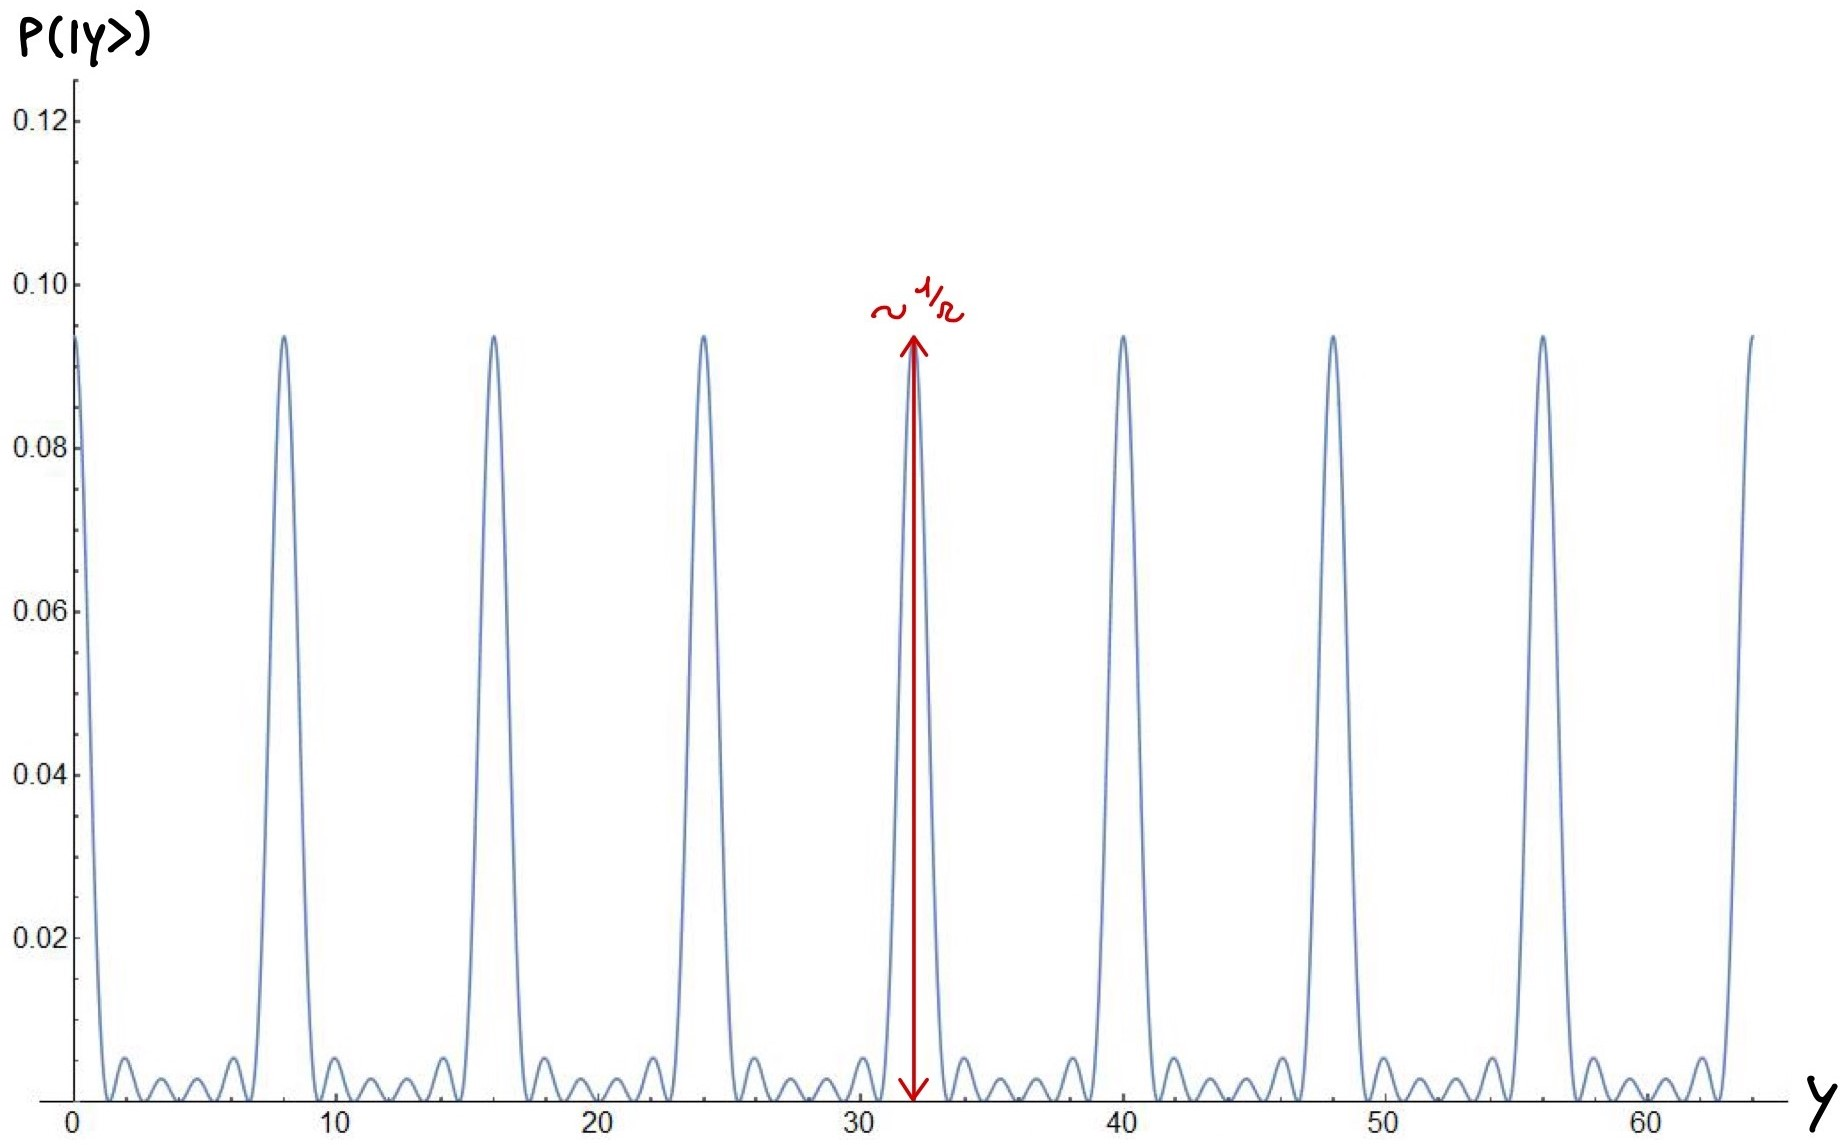
\includegraphics[scale=0.325]{images/probability_y}
    \caption{Esempio di grafico della probabilità di misurare $y$ della formula \eqref{probability_y}, dove $0 \leqslant y \leqslant 2^n$. In questo esempio si è usato $n = m = 6$ e $r = 8$. Si noti come il numero di picchi sia $\order{r}$ e la loro altezza, come ordine di grandezza, comparabile a $1/r$.}
    \label{fig:probability_y}
\end{figure}
Notiamo che vi sono differenti picchi di diverse ampiezze: ciò è dovuto al fatto che ci sono valori di $y$ dove abbiamo interferenza costruttiva, mentre in altri si ha interferenza distruttiva. Nel realizzare tale grafico, però, abbiamo assunto che $y \in \mathbb{R}$, ma bisogna ricordare che $y\in \mathbb{Z}$, quindi si tratta di un'approssimazione perché non tutti i punti della curva devono essere disegnati ! In realtà, per valori di $n$ molto grandi $2^n$ è enorme quindi la discretizzazione è minima e quasi impercettibile. I punti in cui la probabilità è maggiore, in corrispondenza dei picchi più alti, si ha $y = j\frac{2^n}{r}$ dove $j \in \mathbb{N}$. Per tali valori, gli esponenziali dentro la probabilità in \eqref{probability_y} non sono altro che $e^{2\pi i j k}=1$ perché $j, k \in \mathbb{Z}$, quindi la \eqref{probability_y} diventa:
\begin{equation*}
    P(\ket{y}) = \frac{1}{m 2^n} \abs{\sum_{k=0}^{m-1} 1}^2 = \frac{m^2}{m2^n} = \frac{m}{2^n} \, ,
\end{equation*}
il quale è il valore massimo della probabilità. Per capire per quale ragione abbiamo indicato nel grafico \ref{fig:probability_y} che l'altezza dei picchi è di circa $1/r$, ricordiamo che $2^n \sim N^2$, $r \sim N$ e anche $m \sim N$, per cui:
\begin{equation*}
    P(\ket{y}) = \frac{m}{2^n} \sim \frac N{N^2} \sim \frac 1 N \sim \frac 1 r \, .
\end{equation*}
Notiamo che sebbene abbiamo disegnato una funzione continua, l'approssimazione è comunque molto buona perché la probabilità totale è correttamente normalizzata a 1: infatti l'altezza dei picchi per il loro numero non è altro che $\frac{1}{r} \times m \sim \frac{1}{r} \times r \simeq 1$, quindi gran parte della probabilità è saturata i corrispondenza dei picchi (si può dimostrare che nel limite in cui $n \to \infty$ i picchi tendono a delle delta function). 

\noindent Un risultato fondamentale è che passando attraverso delle manipolazioni algebriche di seno e coseno, si può dimostrare che si ha circa il $40$\% di possibilità ($P(\ket{y}) = \frac{4}{\pi^2}$) di misurare $y$ e ottenere un valore che si trovi in prossimità di uno di questi picchi con un errore di circa $\frac 12$: ricordando che i picchi sono situati in $y = j \frac{2^n}{r}$, possiamo formalmente scrivere che
\begin{equation}
    \abs{y-j\frac{2^n}{r}} < \frac 12 \, , \quad \Rightarrow \quad 
    \abs{\frac y{2^n}-\frac jr} < \frac 1{2^{n+1}} \, ,
    \label{eq:shor2}
\end{equation}
dove abbiamo diviso per $2^n$. Stiamo quindi dicendo che una misura di $y$ soddisfa la disuguaglianza \eqref{eq:shor2} il 40\% delle volte. Possiamo estrarre $r$ dalla \eqref{eq:shor2} ? Innanzitutto notiamo che, essendo $0 \leqslant y \leqslant 2^n$, abbiamo $0 \leqslant \frac{y}{2^n} \leqslant 1$. Se $n = 2 n_0$ allora avremo $2^{n}=2^{2n_0}=N^2$, quindi quando la \eqref{eq:shor2} è verificata esiste un singolo numero razionale della forma $\frac j r$ che la  soddisfa e dal quale è possibile estrarre $r$. 

\noindent La logica è mostrata nel disegno della figura \ref{fig:inequality_40}: prendeno il segmento $[0,1]$ e suddividendolo in step uguali di lunghezza $\frac{1}{2^n}$, possiamo rappresentare con delle barrette verticali tutti i possibili valori di $y$ tali che $0 \leqslant \frac{y}{2^n} \leqslant 1$. La disuguaglianza \eqref{eq:shor2} ci dice che il numero $\frac{j}{r}$ (indicato con una "$\times$" azzurra) è vicino a $\frac{y}{2^n}$ con una distanza minore di $\frac{1}{2^{n+1}}$. 
\begin{figure}[!h]
    \centering
    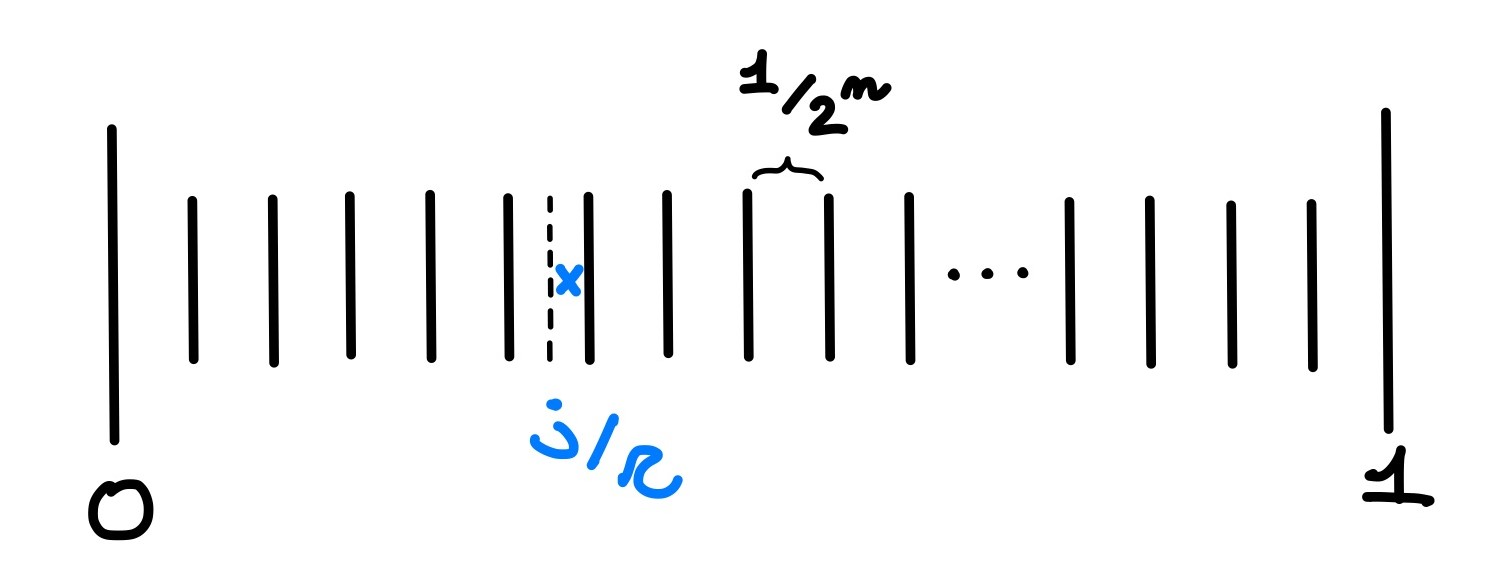
\includegraphics[scale=0.3]{images/inequality_40}
    \caption{Rappresentazione geometrica della disuguaglianza \eqref{eq:shor2}.}
    \label{fig:inequality_40}
\end{figure}

\noindent La domanda che possiamo porci è se esista più di un numero razionale che soddisfi questa particolare proprietà. Supponiamo per assurdo che esistano due numeri razionali $\frac{j_1}{r_1}$ e $\frac{j_2}{r_2}$ che soddisfano la disuguaglianza \eqref{eq:shor2} (e la condizione per cui $r_1, r_2 < N$). Allora la differenza tra questi due numeri è
\begin{equation}\label{difference_rational_numers}
    \frac{j_1}{r_1} - \frac{j_2}{r_2} = \frac{r_2j_1-r_1j_2}{r_1r_1} \, ,
\end{equation}
tuttavia il numeratore è un intero e il denominatore è di ordine $\order{N^2}$: essendo $r_1, r_2 < N$ allora il denominatore è strettamente minore di $N^2$ quindi la \eqref{difference_rational_numers} è $\geqslant \frac 1{N^2} = \frac{1}{2^n}$, che è proprio la larghezza degli step in cui abbiamo suddiviso $[0,1]$. Questo significa che se ci sono due soluzioni della \eqref{eq:shor2} allora la distanza tra le due deve necessariamente essere più grande della misura dello step: in un dato step è possibile trovare una sola soluzione, ossia un solo numero razionale che verifica la \eqref{eq:shor2}.

\noindent Riassumendo: misurando un valore $y$ che soddisfa la \eqref{eq:shor2} otteniamo un unico numero razionale $\frac{j}{r}$. Il punto chiave è quindi trovare  $\frac jr$, tuttavia questo non è così semplice, perché quello che si ottiene dalla misura è un numero scritto in forma decimale, il quale vorremmo poterlo scrivere come rapporto tra razionali. Nonostante ciò facciamo uso del seguente risultato di teoria dei numeri che non dimostreremo. Riscriviamo la disuguaglianza \eqref{eq:shor2} come
\begin{equation*}
    \abs{x-\frac jr} \leqslant \frac 1{2r^2} \, , \; \text{ dove } x\in[0,1] \, .
\end{equation*}
Il valore $x$ è dato dalla misura mentre lo scopo è quello di trovare un numero razionale $\frac jr$ che soddisfi questa disuguaglianza. Il risultato dalla teoria dei numeri asserisce che questo valore appare nell'espansione in frazione continua del numero $x$:
\begin{equation*}
    x=\frac{1}{x_0+\frac{1}{x_1+\frac{1}{x_2+\ldots}}} \, .
\end{equation*}

\begin{esempio}[Espansione in frazione continua]
    Supponiamo di considerare il numero $x=0.256789$. Prendendone l'inverso avremo $\frac{1}{x} = \frac{1}{0.256789} = 3.8942478 \ldots$. Da questo risultato è evidente che $x_0 = 3$. Nello step successivo si calcola $x_1$: calcoliamo $\frac{1}{x}-3$ e poi $\left( \frac{1}{x}-3 \right)^{-1}$, la cui parte intera è $x_1$. Iterando all'infinito questo procedimento si ottiene l'espansione in frazione continua di $x$:
    \begin{equation*}
        x=\frac{1}{3+\frac{1}{1+\frac{1}{8+\dots}}} \, .
    \end{equation*}
    Ad ogni step si ottiene quindi un'approssimazione razionale di $x$, infatti il set di numeri razionali che approssimano il suo valore è dato da $\left\{ \frac 13, \frac 14, \frac 9{35}, \frac {19}{74}, \frac{104}{405}, \dots \right\}$. Più si procede, meglio approssimato sarà il valore di $x$. Il teorema ci dice che a un certo punto possiamo trovare il valore di $\frac jr$ all'interno di questo insieme e questo con una probabilità del 100\%. 
\end{esempio}

\noindent Tuttavia di questo procedimento vanno fatte delle opportune precisazioni:
\begin{itemize}
    \item Supponiamo che $j$ e $r$ abbiano dei fattori comuni (e questo ovviamente non lo sapremo mai), allora il valore di $r$ può essere diverso, infatti:
    \begin{equation*}
        \frac jr=\frac{j_0k}{r_0k}=\frac{j_0}{r_0} \, ,
    \end{equation*}
    quindi mediante la procedura sopraelencata, al posto di trovare il periodo cercato, si ottiene $r_0$. Nonostante ciò si è trovato un divisore di $r$, quindi prendendo la forma analitica di $f$ si può provare a calcolare $f(x+r_0)$, $f(x + 2 r_0)$, $f(x + 3 r_0)$, \dots fino a quando effettivamente si trova un valore uguale a  $f(x)$.
    
    \item Talvolta si possono misurare dei valori $y$ che non soddisfano la disuguaglianza \eqref{eq:shor2} (la probabilità di soddisfarla è infatti del 40\%). In tal caso basta semplicemente ricominciare l'algoritmo da capo con una nuova esecuzione del circuito e della QFT fino a quando non si ottiene un valore di $y$ che soddisfi la \eqref{eq:shor2}. Inoltre è possibile dimostrare che la probabilità che la \eqref{eq:shor2} sia soddisfatta cresce fino al 90\% se si sa a priori che $r < \frac N2$.
\end{itemize}
Concludiamo la discussione dicendo che lo stesso tipo di algoritmo può essere utilizzato per calcolare i \textit{logaritmi discreti}, oppure per la simulazione di sistemi quantistici (si possono calcolare gli autovalori di matrici unitarie molto grandi che servono per il calcolo degli autovalori delle relative hamiltoniane e degli evoluti temporali).
    \vspace{0.5cm}

\noindent  \lecture{8}{2/11/2021}

\section{Misurazioni indirette}\label{sec:mis_ind}

Per ora abbiamo analizzato il problema di \textit{cosa} avviene al sistema successivamente a una misurazione. Tuttavia non abbiamo ancora cercato di spiegare \textit{come} avviene una misurazione.
Generalmente, fra l'osservatore e il sistema quantistico, vi è un cosiddetto dispositivo classico di misura (\textit{classical measuring device})\footnote{Esempi di dispositivi di questo tipo sono le foto-emulsioni, la camera a nebbia di Wilson etc. etc.}. Le misurazioni in cui un dispositivo di misura classico interagisce propriamente con l'oggetto quantistico studiato vengono chiamate \textbf{misure dirette}. 
Chiaramente, in una misura di questo genere, stiamo utilizzando un sistema a molti gradi di libertà che vanno inevitabilmente a perturbare fortemente il sistema (abbiamo perturbazioni ben più grandi di quelle previste dai limiti di Heisenberg). Inoltre è raro che il sistema modifichi unicamente il grado di libertà studiato: con ogni probabilità porterà a una grossa perturbazione su una vasta gamma di osservabili.
Per questo si tende a preferire quelle che vengono chiamate \textbf{misure indirette}. Tali misurazioni sfruttano una sonda quantistica (\textit{quantum probe}) per mediare l'interazione sistema classico - sistema quantistico.
Abbiamo un processo a due fasi:
\begin{enumerate}
    \item la sonda quantistica interagisce con l'oggetto da misurare e fra di essi si stabilisce una correlazione;
    \item la sonda viene rilevata e misurata direttamente da un dispositivo classico.
\end{enumerate}
\noindent La sonda viene preparata in modo adeguato quando è ancora del tutto sconnessa al sistema e ha, in particolare, un osservabile detto \textbf{\textit{pointer observable}} che ha un legame con l'osservabile d'interesse nel sistema quantistico: ovvero c'è un rapporto (idealmente 1:1) fra i valori dei due osservabili.
Durante l'interazione sonda - sistema, d'altro canto, dobbiamo aspettarci che i due sistemi diventino \textit{entangled} e questo limiterà parzialmente la nostra misura finale: benché possiamo pensare di avere alte perturbazioni nella seconda fase del processo (perché non ci interessa conservare la sonda) dovremo limitarci per non perturbare troppo il sistema originale.
Per raggiungere un'alta precisione nel processo di misura cercheremo di rispettare sempre due semplici condizioni:
\begin{itemize}
    \item il secondo step della misurazione deve avvenire solo quando il primo risulta completato;
    \item il secondo step non deve contribuire significativamente all'errore totale della misura.
\end{itemize}
Se seguiamo queste regole, dunque, le uniche fonti di errore nella misura e le sole perturbazioni del sistema saranno quelle relative a incertezze intrinseche al processo di preparazione della sonda\footnote{Non stiamo considerando interazioni coi gradi di libertà ambientali.}.
\vspace{1cm}
\noindent Analizziamo, dunque, il processo di misura.
Abbiamo due differenti sistemi quantistici (la sonda e l'oggetto studiato) descritti dalle rispettive matrici densità $\hat \rho _P$ e $\hat \rho _{INIT}$. L'evoluzione di entrambe può essere descritta introducendo $\hat U (t) = e^{-\frac{i}{\hbar}\hat H t}$ dove $\hat H$ è l'hamiltoniana totale del sistema ($\hat H = \hat H_{probe} + \hat H _{obj} + \hat H _{interaction}$):
\begin{equation*}
    (\hat \rho_P \hat \rho_{init})'=\hat U (t) \hat \rho_P \hat \rho_{init} \hat U ^\dagger (t)
\end{equation*}
\noindent Abbiamo detto che il processo di misurazione non è unitario, ma a questo punto la non-unitarietà è tutta contenuta nella fase di interazione fra sonda e strumentazione di misura.
Lo stato finale della sonda, dopo l'interazione, è dato dalla seguente formula:
\begin{equation*}
    \hat \rho_{probe}' = \Tr_{obj} \left( \hat U \hat \rho_{probe} \hat \rho_{int} \hat U ^\dagger \right)
\end{equation*}
\noindent Solo a questo punto utilizziamo una misura proiettiva sulla sonda. 
Misuriamo il \textit{pointer observable} $P\tilde a$ nello spazio della sonda che è collegato con l'osservabile $A$ nello spazio dell'oggetto studiato. Avremo l'autostato dell'operatore puntatore: $\ket{\tilde a}$ che corrisponderà all'autovalore (e rispettivo autostato) $\tilde a$ per l'oggetto.
La probabilità di avere un certo autovalore sarà:
\begin{equation*}
    P(\tilde a) = \Tr \left( \ket{\tilde a}\bra{\tilde a} \hat \rho_{probe}'\right)
\end{equation*}
E la traccia che scriviamo qui è una traccia totale che opera nello spazio della sonda.
Possiamo riscrivere questa equazione:
\begin{equation*}
    P(\tilde a) = \Tr \left( \hat \Pi (\tilde a) \rho_{init} \right)
\end{equation*}
Dove, a questo punto, la traccia opera solo sullo spazio dell'oggetto e abbiamo introdotto l'operatore $\hat \Pi$ (anch'esso opera sullo spazio dell'oggetto)  che definiamo come:
\begin{equation*}
    \hat \Pi (\tilde a) = \Tr_{probe}\left( \hat U ^\dagger \ket{\tilde a}\bra{\tilde a}\hat U \hat \rho_{probe}  \right)
\end{equation*}
A questo punto l'operatore $\hat \Pi$ contiene lo stato in cui la sonda è preparata ($\hat \rho_{probe}$), lo stato finale della sonda ($\ket{\tilde a}\bra{\tilde a}$) e l'evoluzione temporale (che è l'unico operatore che operava sia sullo spazio della sonda, dipendenza eliminata dalla traccia parziale, che sullo spazio dell'oggetto).
Abbiamo visto la misura dal punto di vista della sonda, ma cosa sta succedendo al nostro oggetto?
Avevamo scritto l'equazione \ref{eq:prob_omega} rimandandone la dimostrazione che, però, vediamo ora.
Possiamo scrivere la matrice finale dell'oggetto (post interazione):
\begin{equation*}
    \hat \rho_{fin} (\tilde a) = \frac{1}{P(\tilde a)}\bra{\tilde a}\hat U \hat \rho_{probe}\hat \rho_{init} \hat U^\dagger \ket{\tilde a}
\end{equation*}
Se possiamo scrivere lo stato iniziale della sonda come: $\hat \rho_{probe} = \sum_i w_i \ket{\psi_i}\bra{\psi_i}$ arriviamo facilmente, per sostituzione, a:
\begin{equation*}
    \hat \rho_{fin} (\tilde a) = \frac{1}{P(\tilde a)} \sum_i \bra{\tilde a}\hat U \ket{\psi_i}\hat \rho_{init} \bra{\psi_i}\hat U ^\dagger \ket{\tilde a}
\end{equation*}
E ricordiamo che $\ket{\tilde a}$ e $\ket{\psi_i}$ sono stati della sonda e $\hat U$ agisce su entrambi gli stati. Dunque gli operatori $\bra{}\hat U \ket{}$ sono operatori dell'oggetto.
Se la sonda si trova, inizialmente, in uno stato puro $\hat \rho_{probe} = \ket{\psi}\bra{\psi}$, allora abbiamo:
\begin{equation*}
    \hat \rho_{fin} (\tilde a) = \frac{1}{P(\tilde a)}\bra{\tilde a}\hat U \ket{\psi}\hat \rho_{init} \bra{\psi}\hat U ^\dagger \ket{\tilde a}
\end{equation*}
E possiamo identificare:
\begin{equation*}
    \bra{\tilde a} \hat U \ket{\psi} = \hat \Omega = \hat U_{obj}\sqrt{\hat M}
\end{equation*}
Con $\hat U_{obj}$ (diverso dall'operatore $\hat U$ precedente) che contiene le informazioni sulla perturbazione dell'oggetto causata dalla sonda.
\vspace{0.5cm}
Abbiamo già visto che abbiamo una misurazione senza demolizione nel caso in cui $[\hat A, \hat \Omega]=0$ che ora possiamo riscrivere:
\begin{equation*}
    \bra{\tilde a}[\hat A, \hat \Omega] \ket{\psi}=0  
\end{equation*}
Tale equazione deve essere vera per ogni autostato $\ket{\tilde a}$, perciò:
\begin{equation*}
    (\hat A \hat U - \hat U \hat A)\ket{\psi}= 0
\end{equation*}
Se moltiplichiamo per $\hat U^\dagger$ otteniamo:
\begin{equation*}
    \hat U ^\dagger (\hat A \hat U - \hat U \hat A)\ket{\psi}= (\hat U^\dagger \hat A \hat U - \hat A ) \ket{\psi}=0
\end{equation*}
Otteniamo, dunque, questa equazione che è la condizione per avere una QND (\textit{Quantum NonDemolition measurement}). Si noti che l'operatore fra parentesi corrisponde alla variazione dell'osservabile $A$ nella rappresentazione di Heisenberg.
Perché questa condizione sia rispettata vi sono due possibilità:
\begin{itemize}
    \item che valga sempre $\hat U ^\dagger \hat A \hat U-\hat A = 0$;
    \item che lo stato iniziale della sonda sia un autostato della differenza $\hat U^\dagger \hat A \hat U - \hat A$.
\end{itemize}
Il secondo caso non è stato particolarmente analizzato né dal punto di vista sperimentale né da quello teorico, mentre ci si è concentrati sulla prima condizione.
Quest'ultima equivale a richiedere $[\hat A, \hat U] = 0$. Tale condizione è necessaria e sufficiente per avere una misura senza demolizione, ma è generalmente complesso verificare che sia verificata poiché è necessario conoscere l'evoluzione di oggetto e sonda.
Per questo si preferisce richiedere una condizione più forte (sufficiente, ma non necessaria): $[\hat A, \hat H]=0$.
Tipicamente avremo l'hamiltoniana scrivibile come:
\begin{equation*}
    \hat H = \hat H_{obj} + \hat H_{probe}+\hat H_{int}
\end{equation*}
Chiaramente abbiamo immediatamente la commutatività con la parte relativa alla sonda: $[\hat A, \hat H_{probe}]$=0 (poiché $\hat A$ è un osservabile dell'oggetto); mentre dovremo esplicitamente richiedere:
\begin{align}
    [\hat A , \hat H_{obj} ] &= 0\\
    [\hat A , \hat H_{int} ] &= 0
\end{align}
    %%%%%%%%%%%%%
% LECTURE 9 %
%%%%%%%%%%%%%
\chapter{Sistemi aperti}

\lecture{9}{05/11/2021}
\section{Matrice densità}
Il formalismo della \textbf{matrice densità} viene solitamente introdotto per affrontare situazioni in cui sono presenti sia un'incertezza quantistica, intrinseca alla QM, che un'incertezza classica, dovuta all'ignoranza su alcune configurazioni del sistema. Spesso viene introdotta nell'ambito della fisica statistica, tuttavia viene largamente utilizzata anche in altri contesti. 

\noindent Ad esempio: supponiamo di considerare un laboratorio e un ambiente esterno in cui è immerso; spesso, per descrivere la fisica del sistema completo, non si possono tenere in considerazione tutti i gradi di libertà dell'ambiente, così si assume che esista un'opportuna descrizione del laboratorio (nel quale potrebbe esserci un qubit o un apparato sperimentale) più l'ambiente e si prende una traccia (capiremo tra un attimo cosa significhi) su tutti i gradi di libertà dell'ambiente. In questo modo si ottiene una \textbf{descrizione efficace} del laboratorio, la quale contiene "nascosta" la nostra ignoranza relativa all'ambiente. 

\noindent Vediamo la definizione generale:

\begin{definizione}[\textbf{Matrice Densità}]
    Siano $\ket{\psi_i}$ un insieme di stati quantistici con probabilità classica $p_i$ ($\sum_i p_i = 1$), ossia la probabilità di realizzare ogni stato $\ket{\psi_i}$ è data da $p_i$. Indichiamo con $\{ p_i, \ket{\psi_i} \}$ l'insieme di tali stati con le rispettive probabilità (assumiamo che $\braket{\psi_i} = 1$). Si definisce \textbf{matrice densità} (o \textbf{operatore densità}) $\rho$ la seguente
    \begin{equation}\label{density_matrix}
        \rho = \sum_i p_i \ket{\psi_i} \otimes \bra{\psi_i} \, .
    \end{equation}
\end{definizione}

\noindent Si noti che, come evidenziato, le $p_i$ sono probabilità \textit{classiche} poiché è già intrinseca ad ogni stato $\ket{\psi_i}$ la descrizione mediante probabilità \textit{quantistica}. Chiaramente $\rho$, in quanto prodotto esterno, agisce come un operatore sugli stati dello spazio di Hilbert. È importante sottolineare che che gli stati $\ket{\psi_i}$ sono normalizzati ma non necessariamente ortogonali. 

\noindent L'introduzione della \eqref{density_matrix} è utile perché permette di scrivere differenti quantità in forma compatta. Ad esempio, la media di un'osservabile $A$ può essere scritta come
\begin{equation}\label{expval_A_rho}
    \expval{A} = \Tr (\rho A) \, .
\end{equation}
\begin{proof}
    Scriviamo 
    \begin{equation*}
        \Tr (\rho A) = \sum_i p_i \Tr \left( \ketbra{\psi_i} A \right) = \sum_i p_i \expval{A}{\psi_i} = \expval{A} \, ,
    \end{equation*}
    dove nel secondo passaggio abbiamo utilizzato la proprietà ciclica della traccia per muovere il ket a destra. Notiamo che questa operazione può essere svolta per la ragione seguente: in generale per gli operatori si ha $\Tr B = \sum_n \expval{B}{n}$ dove $\{ \ket{n} \}$ è una base ortonormale, perciò nel passaggio sopra possiamo scrivere
    \begin{equation*}
        \Tr \left( \ketbra{\psi_i} A \right) = \sum_n \braket{n}{\psi_i} \mel{\psi_i}{A}{n} = \sum_n \mel{\psi_i}{A}{n} \braket{n}{\psi_i} = \expval{A}{\psi_i} \, ,
    \end{equation*}
    dove nell'ultimo passaggio abbiamo utilizzato la relazione di completezza $\mathbb{I} = \sum_n \ketbra{n}$.
\end{proof}

\noindent Se si possiede solamente uno stato $\ket{\psi}$, esso viene chiamato \textbf{stato puro}, quindi la matrice densità si scriverà come $\rho = \ketbra{\psi}$. Al contrario, un insieme di stati $\{ p_i, \ket{\psi_i} \}$, con almeno 2 probabilità $p_i \neq 0$, avrà matrice densità $\rho = \sum_i p_i \ketbra{\psi_i}$ ed è chiamato \textbf{stato misto} o \textbf{miscela di stati} (nota anche come \textbf{mixture}). Ribadiamo nuovamente che in quest'ultima situazione l'incertezza classica $p_i$ si va ad aggiungere all'incertezza puramente quantomeccanica degli stati quantistici.

\begin{esempio}[\textbf{Miscela in Meccanica Statistica}]
    Il più semplice esempio di miscela di stati in meccanica statistica è costituito dall'insieme di stati $\{ E_n, \ket{n} \}$, dove $H \ket{n} = E_n \ket{n}$, in cui assegniamo ad ogni stato una probabilità classica 
    \begin{equation*}
        P(E_n) = \frac{e^{-\frac{E_n}{k_BT}}}{Z} \, , \; \text{ con } \; Z = \sum_n e^{-\frac{E_n}{k_BT}} \, ,
    \end{equation*}
    dove $Z$ è chiamata \textbf{funzione di partizione}. Quindi per studiare un tale sistema dal punto di vista quantistico possiamo dire che in aggiunta all'incertezza quantistica ci sono altre probabilità classiche $P(E_n)$ dipendenti dalla temperatura. Per un tale sistema la matrice densità non è altro che
    \begin{equation*}
        \rho = \sum_n p_n \ketbra{n} \, , \; \text{ dove } \; p_n \equiv P(E_n) = \frac{e^{-\frac{E_n}{k_BT}}}{Z} \, . 
    \end{equation*}
\end{esempio}

\noindent Vediamo immediatamente l'esempio dei qubit per capire la differenza della matrice densità nel caso di uno stato puro e per miscele di stati:

\begin{esempio}[\textbf{Singolo qubit: stato puro}]
    Immaginiamo un qubit nello stato $\ket{0}$. La matrice \eqref{density_matrix} non è altro che
    \begin{equation*}
        \rho = \ketbra{0} = 
        \begin{pmatrix}
            1 \\ 0
        \end{pmatrix} \otimes 
        \begin{pmatrix}
            1 & 0
        \end{pmatrix} 
        = 
        \begin{pmatrix}
            1 & 0 \\ 0 & 0
        \end{pmatrix} \, ,
    \end{equation*}
    dove nell'ultimo passaggio abbiamo utilizzato il prodotto di Kronecker della definizione \ref{def:Kronecker}.
\end{esempio}

\begin{esempio}[\textbf{Singolo qubit: miscela di stati}]\label{example:mixture_qubit}
    Si consideri un qubit nella miscela di stati in cui $\ket{0}$ è dato con probabilità $p$ e $\ket{1}$ con probabilità $1-p$ (non stiamo prendendo la solita sovrapposizione di stati della QM). Allora la matrice densità risulterà
    \begin{equation*}
        \rho = p \ketbra{0} + (1-p) \ketbra{1} = p 
        \begin{pmatrix}
            1 & 0 \\ 0 & 0
        \end{pmatrix} + 
        (1-p)
        \begin{pmatrix}
            0 & 0 \\ 0 & 1
        \end{pmatrix}
        =
        \begin{pmatrix}
            p & 0 \\ 0 & 1-p
        \end{pmatrix} \, .
    \end{equation*} 
\end{esempio}

\noindent Notiamo che dal punto di vista dell'informazione, nello stato puro la matrice densità ha solamente un'entrata: non vi è alcuna incertezza classica (solamente quantistica). Al contrario, per la miscela di stati abbiamo il caso della maggior incertezza possibile quando $p = \frac{1}{2}$ perché $\rho = \frac{1}{2} \mathbb{I}$. In generale, per matrici diagonali,  sono miscele le configurazioni in cui pi\`u di un'entrata diagonale \`e non nulla. Si noti dall'esempio \ref{example:mixture_qubit} che sulle entrate diagonali di $\rho$ si può leggere l'incertezza classica collegata agli stati $\ket{0}$ e $\ket{1}$. 

\noindent Questi esempi erano molto semplici perché $\rho$ è diagonale: la matrice densità non è in generale diagonale né per gli stati puri né per le miscele. Vediamo alcuni esempi:

\begin{esempio}[\textbf{Stato puro: $\rho$ non diagonale}]\label{example:rho_non_diagonal_pure}
    Consideriamo il caso dello stato puro di un qubit nella sua forma più generale, ossia $\ket{\psi} = \alpha \ket{0} + \beta \ket{1}$. La \eqref{density_matrix} diventa una matrice non diagonale, infatti
    \begin{equation*}
        \rho = \ketbra{\psi} = 
        \begin{pmatrix}
            \alpha \\ \beta
        \end{pmatrix}
        \otimes
        \begin{pmatrix}
            \alpha^\ast & \beta^\ast
        \end{pmatrix} 
        = 
        \begin{pmatrix}
            \abs{\alpha}^2 & \alpha \beta^\ast \\ \alpha^\ast \beta & \abs{\beta}^2
        \end{pmatrix} \, .
    \end{equation*}
\end{esempio}

\noindent Si noti dall'esempio precedente la differenza tra le entrate diagonali e non: su quelle diagonali vi sono le probabilità quantistiche del risultato di una misura, mentre su quelle non diagonali sono presenti dei prodotti tra $\alpha$ e $\beta$ che misurano, in un certo senso, l'interferenza (sovrapposizione) tra $\ket{0}$ e $\ket{1}$.

\begin{esempio}[\textbf{Miscela: $\rho$ non diagonale}]\label{example:rho_non_diagonal_mixture}
    Supponiamo di avere la miscela costituita dal 50\% di probabilità di avere $\ket{0}$ e dal $50\%$ di probabilità di avere $\ket{+} = \frac{1}{\sqrt{2}} (\ket{0} + \ket{1})$. In questo caso $\rho$ non è diagonale ed è data da una combinazione lineare di stati non ortogonali:
    \begin{equation*}
        \rho = \frac{1}{2} \ketbra{0} + \frac{1}{2} \ketbra{+} = \frac{1}{2} \begin{pmatrix} 1 & 0 \\ 0 & 0 \end{pmatrix} + \frac{1}{4} \begin{pmatrix} 1 \\ 1 \end{pmatrix} \otimes \begin{pmatrix} 1 & 1 \end{pmatrix} = \begin{pmatrix} \frac{3}{4} & \frac{1}{4} \\ \frac{1}{4} & \frac{1}{4} \end{pmatrix} \, . 
    \end{equation*}
\end{esempio}

\noindent Vediamo alcune proprietà generali della matrice densità:
\begin{enumerate}
    \item \textit{$\rho$ è hermitiana e positiva}. 
    \begin{proof}
        Ricordando che $p_i \geq 0 \in \mathbb{R}$ allora
        \begin{equation*}
            \left( \sum_i p_i \ketbra{\psi_i} \right)^\dag = \sum_i p_i \ketbra{\psi_i} \, .
        \end{equation*}
        La positività di un operatore $A$ è data dalla proprietà $\expval{A}{\phi} \geq 0$ per ogni $\ket{\phi}$, quindi
        \begin{equation*}
            \expval{\rho}{\phi} = \bra{\phi} \sum_i p_i \ket{\psi_i} \braket{\psi_i}{\phi} = \sum_i p_i \braket{\phi}{\psi_i} \underbrace{\braket{\psi_i}{\phi}}_{\braket{\phi}{\psi_i}^\ast} = \sum_i p_i \abs{\braket{\phi}{\psi_i}}^2 \geq 0 \, .
        \end{equation*}
    \end{proof}
    
    \item $\Tr \rho = 1$.
    \begin{proof}
        \begin{equation*}
            \Tr \left[ \sum_i p_i \ketbra{\psi_i} \right] = \sum_i p_i \Tr \ketbra{\psi_i} = \sum_i p_i \braket{\psi_i} = 1 \, ,
        \end{equation*}
        dove nel penultimo passaggio abbiamo usato la proprietà ciclica della traccia come nella dimostrazione della \eqref{expval_A_rho}.
    \end{proof}
    
    \item \textit{$\Tr \rho^2 \leq 1$ e $\Tr \rho^2 = 1$ solo per gli stati puri}.
    \begin{proof}
        Dato che $\rho$ è hermitiana allora può essere diagonalizzata, quindi $\rho \ket{n} = \rho_n \ket{n}$. In particolare avremo
        \begin{equation}\label{diagonalization_rho}
            \rho = \sum_i p_i \ketbra{\psi_i} \equiv \sum_n \rho_n \ketbra{n} \, ;
        \end{equation}
        quindi la matrice densità è scrivibile come somma del prodotto tra i proiettori nella direzione degli autospazi e dei corrispondenti autovalori. Notiamo che la formula precedente consiste di fatto nella diagonalizzazione in notazione di Dirac. Chiaramente in generale $p_i \neq \rho_i$! Dato che $\Tr \rho = 1$ allora dalla precedente si ha che $\sum_n \rho_n = 1$. Cerchiamo di valutare $\Tr \rho^2 = \sum_n \rho_n^2$: dato che la matrice densità è hermitiana e positiva allora $\rho_n \geq 0 \in \mathbb{R}$, ma al tempo stesso si deve avere $0 \leq \rho_n \leq 1$ poiché $\sum_n \rho_n = 1$. Ma allora
        \begin{equation*}
            0 \leq \rho_n^2 \leq \rho_n \leq 1 \, , \quad \Rightarrow \quad \sum_n \rho_n^2 \leq \sum_n \rho_n = 1 \, .
        \end{equation*}
        Il caso limite è dato da
        \begin{equation*}
            \sum_n \rho_n^2 = 1 = \sum_n \rho_n \quad \Leftrightarrow \quad \rho_n = \rho_n^2 \, , \; \forall n \, ,
        \end{equation*}
        ma per numeri tra 0 e 1 questo è vero solamente per $\rho_n = 1 \lor \rho_n = 0$: solamente un valore è diverso da 0 (uguale a 1) mentre tutti gli altri sono 0, quindi $\rho = \ketbra{n}$ per un particolare $n$, ossia si tratta di uno stato puro. 
    \end{proof}
    Si noti che la formula $\left[ \Tr \rho^2 = 1 \Leftrightarrow \text{ stato puro} \right]$ è un criterio per stabilire se effettivamente uno stato è puro. Inoltre, essendo $\rho$ hermitiana, può sempre essere diagonalizzata secondo la \eqref{diagonalization_rho} e quindi la sua forma non è unica (si pensi ai casi degli esempi \ref{example:rho_non_diagonal_pure} e \ref{example:rho_non_diagonal_mixture} che possono essere diagonalizzati).
\end{enumerate}

\noindent Torniamo al caso dei qubit. Avevamo visto che la più generale matrice hermitiana $2 \times 2$ può essere scritta come $\rho = a_0 \mathbb{I} + \vec{a} \cdot \vec{\sigma}$ con $a_0, \vec{a} \in \mathbb{R}$, ma $\Tr \rho = 1$ e quindi, dato che le matrici di Pauli hanno traccia nulla, avremo $1 = 2 a_0$, ossia $a_0 = \frac{1}{2}$. Possiamo allora scrivere la matrice densità come
\begin{equation}\label{density_matrix_Pauli}
    \rho = \frac{\mathbb{I} + \vec{r} \cdot \vec{\sigma}}{2} \, , \; \text{ dove } \; r_i \in \mathbb{R} \, .
\end{equation}
Quali sono gli autovalori di $\rho$? Sappiamo che $\vec{r} \cdot \vec{\sigma}$ è lo spin in direzione $\vec{r}$, il quale ha autovalori $\abs{\vec{r}\,}$ e $-\abs{\vec{r}\,}$, inoltre $\rho$ è hermitiana, quindi
\begin{equation*}
    \eig(\rho) \equiv \lambda = \frac{1 \pm \abs{\vec{r} \,}}{2} \geq 0 \, , \quad \Rightarrow \quad \abs{\vec{r}\,} \leq 1 \, . 
\end{equation*}
Calcoliamo ora $\Tr \rho^2$ sempre usando la \eqref{density_matrix_Pauli}:
\begin{equation*}
    \Tr \rho^2 = \Tr \left[ \frac{1}{4} \left( \mathbb{I} + 2 \vec{r} \cdot \vec{\sigma} + \abs{\vec{r}\,}^2 \right) \right] = \frac{1 + \abs{\vec{r}\,}^2}{2} \leq 1 \, ,
\end{equation*}
dove abbiamo usato il risultato seguente
\begin{equation*}
    r_i r_j \sigma_i \sigma_j = r_i r_j \left( \delta_{ij} \mathbb{I} + i \varepsilon_{ijk} \sigma_k \right) = \abs{\vec{r}\,}^2 + i (\varepsilon_{kij} r_i r_j) \sigma_k = \abs{\vec{r}\,}^2 + i \underbrace{(\vec{r} \times \vec{r}\,)}_0 \cdot \, \vec{\sigma} = \abs{\vec{r}\,}^2 \, .
\end{equation*}
Notiamo che per gli stati puri $\frac{1+ \abs{\vec{r}\,}^2}{2} = 1 \Leftrightarrow \abs{\vec{r}\,}^2 = 1$, quindi possiamo impiegare nuovamente la descrizione grafica con la sfera di Bloch che abbiamo introdotto nella Sottosezione \ref{subsec:Bloch}. Associamo il punto dato da $\vec{r}$ con la matrice densità \eqref{density_matrix_Pauli} in maniera tale da estendere questa descrizione anche ai punti interni della sfera (si veda la Figura \ref{fig:BlochSphere} a Pagina \pageref{fig:BlochSphere}): i punti sulla superficie sono stati puri, mentre quelli all'interno sono delle miscele di stati. Tenendo presente la Figura \ref{fig:BlochSphere2} a Pagina \pageref{fig:BlochSphere2}, focalizziamo la nostra attenzione su due direzioni precise:
\begin{itemize}
    \item Consideriamo l'asse $z$: in tal caso avremo $\vec{r} = (0, 0, r)$ con $r \in [-1, 1]$. Chiaramente i due stati corrispondenti ai punti sulla superficie sono $\ket{0}$ per $z=1$ e $\ket{1}$ per $z = -1$. La matrice densità non è altro che
    \begin{equation}\label{rho_z_Bloch}
        \rho = \frac{\mathbb{I}}{2} + \frac{r}{2} \sigma_3 = 
        \begin{pmatrix}
            \frac{1+r}{2} & 0 \\ 0 & \frac{1-r}{2}
        \end{pmatrix}
        \equiv
        \begin{pmatrix}
            p & 0 \\ 0 & 1-p
        \end{pmatrix} \, , \; \text{ con } \; p = \frac{1+r}{2} \, ;
    \end{equation}
    si tratta della stessa forma dell'Esempio \ref{example:mixture_qubit}: si ha una miscela di stati con probabilità classiche $p$ di avere $\ket{0}$ e $1-p$ di avere $\ket{1}$. 
    
    \item Consideriamo ora, invece, l'asse $x$: in tal caso $\vec{r} = (r, 0, 0)$ e gli stati sulla superficie (intersezione sfera con asse $x$) sono $\ket{+}$ per $x = 1$ e $\ket{-}$ per $x = -1$. La \eqref{density_matrix_Pauli} non è altro che
    \begin{equation}\label{rho_x_Bloch}
        \rho = \frac{\mathbb{I}}{2} + \frac{r}{2} \sigma_1 =
        \begin{pmatrix}
            \frac{1}{2} & \frac{r}{2} \\ \frac{r}{2} & \frac{1}{2}
        \end{pmatrix} \, ;
    \end{equation}
    perciò i punti corrispondenti a $\ket{+}$ e $\ket{-}$ sono gli stati puri nella direzione in cui si sta misurando lo spin, mentre tutti gli altri punti intermedi lungo $x$ sono una miscela di $\ket{+}$ e $\ket{-}$. 
\end{itemize}

\noindent Notiamo che il punto $\vec{r} = 0$ è l'unico punto comune a tutti e 3 gli intervalli nelle 3 direzioni spaziali: esso corrisponde alla massima indeterminazione possibile, infatti
\begin{equation*}
    \rho = \frac{\mathbb{I}}{2} = 
    \begin{pmatrix}
        \frac{1}{2} & 0 \\ 0 & \frac{1}{2}
    \end{pmatrix} \, ,
\end{equation*}
il quale non è altro che una sovrapposizione dei due autostati corrispondenti ognuno una probabilità classica del 50\%. Un fatto importante da sottolineare è che la matrice precedente può essere ottenuta sia dalla \eqref{rho_z_Bloch} che dalla \eqref{rho_x_Bloch} ponendo $p = \frac{1}{2}$ e $r = 0$: solamente conoscendo la matrice densità di un sistema non siamo in grado di distinguere la miscela di stati in cui ci troviamo!

\section{Sottosistemi e traccia parziale}
Torniamo ad affrontare alcuni casi interessanti dal punto di vista della fisica dei qubit. Il formalismo della matrice densità risulta utile quando si hanno sistemi bipartiti tali che $\mathcal{H} = \mathcal{H}_A \otimes \mathcal{H}_B$. Supponiamo che Alice si trovi in un laboratorio descritto da $\mathcal{H}_A$ e che Bob invece sia in un altro laboratorio descritto da $\mathcal{H}_B$: la matrice densità è utile quando si vuole studiare la fisica dal punto di vista di Alice, la quale ignora il laboratorio di Bob; Alice vorrebbe ignorare parte dello spazio di Hilbert totale perché non ne ha l'accesso completo.  Questo fatto, vedremo, porta ad una descrizione fisica in termini di miscele di stati anche se si era partiti da uno stato puro in $\mathcal{H}$. 

\noindent Che cosa significa fare esperimenti dal punto di vista di Alice? Significa che Alice effettua misure di osservabili della forma $O = O_A \otimes \mathbb{I}_B$, quindi agisce solamente nel proprio laboratorio senza fare nulla sul laboratorio di Bob. Immaginiamo che i due laboratori siano soggetti a dell'indeterminazione classica, quindi il sistema totale è ben descritto da un'opportuna matrice densità $\rho$. Siamo interessati al sottosistema descritto da $\mathcal{H}_A$: chiamiamo $\{ \ket{nm} \}$ la base dello spazio di Hilbert totale $\mathcal{H}$ dove $\ket{nm} \equiv \ket{n}_A \otimes \ket{m}_B$ con $\ket{n}_A \in \mathcal{H}_A$ e $\ket{m}_B \in \mathcal{H}_B$. Calcoliamo il valor medio di $O$ mediante la \eqref{expval_A_rho}:
\begin{align*}
    \expval{O} &= \Tr (O \rho) = \sum_{n,m} \expval{O \rho}{nm} \\
    &= \sum_{\substack{n,m \\ n', m'}} \mel{nm}{O_A \otimes \mathbb{I}_B}{n'm'} \mel{n'm'}{\rho}{nm} \\
    &= \sum_{\substack{n,m \\ n', m'}} \mel{n}{O_A}{n'} \underbrace{\braket{m}{m'}}_{\delta_{mm'}} \mel{n'm'}{\rho}{nm} \\
    &= \sum_{n,m,n'} \mel{n}{O_A}{n'} \mel{n'm}{\rho}{nm} \\
    &= \sum_{n,n'} \mel{n}{O_A}{n'} \sum_m \mel{n'm}{\rho}{nm} \, ,
\end{align*}
dove nella seconda riga abbiamo inserito una relazione di completezza nello spazio $\mathcal{H}$: $\mathbb{I} = \sum_{n',m'} \ketbra{n'm'}$. Definiamo ora il seguente oggetto
\begin{equation}\label{rho_A}
    \mel{n'}{\rho_A}{n} \equiv \sum_m \mel{n'm}{\rho}{nm} \, ,
\end{equation}
dove chiaramente $\rho_A$ agisce solamente su $\mathcal{H}_A$. In questo modo la precedente diventa
\begin{equation*}
    \expval{O} = \sum_{n,n'} \mel{n}{O_A}{n'} \mel{n'}{\rho_A}{n} = \sum_n \expval{O_A \rho_A}{n} = \Tr (O_A \rho_A) \, ,
\end{equation*}
dove abbiamo tolto, nel penultimo passaggio, una relazione di completezza in $\mathcal{H}_A$. In definitiva abbiamo ricavato
\begin{equation}\label{expval_O_partial_trace}
    \expval{O} = \Tr (O_A \rho_A) \, .
\end{equation}
Siamo partiti dal considerare un valor medio di una grandezza di tutto lo spazio di Hilbert, ma abbiamo ricavato una formula che considera solamente oggetti che agiscono su $\mathcal{H}_A$! La relazione \eqref{expval_O_partial_trace} permette di dare una \textbf{descrizione efficace} di tutti i gradi di libertà del sistema prendendo una cosiddetta "\textbf{traccia parziale sullo spazio di Hilbert $\mathcal{H}_B$}". 

\noindent Omettendo $n,n'$ ad entrambi i membri, possiamo scrivere la definizione \eqref{rho_A} in forma più compatta come
\begin{equation*}
    \rho_A = \sum_m \expval{\rho}{m} \equiv \Tr_B \rho \, ;
\end{equation*}
risulta ancora più evidente che $\rho_A$ sia costruita prendendo una traccia sui gradi di libertà del laboratorio di Bob, tuttavia notiamo che quest'ultima formula è un po' fuorviante dato che $\rho_A$ è un operatore e il RHS sembrerebbe invece un numero: il simbolo "$\Tr_B$" non produce un numero, bensì un operatore agente unicamente su $\mathcal{H}_A$.

\noindent Vediamo immediatamente due semplici esempi per fissare meglio questi concetti. 
\begin{esempio}[\textbf{Fisica "fattorizzata"}]
    Supponiamo che la fisica di un sistema possa essere "fattorizzata" scrivendo $\rho = \rho_A \otimes \rho_B$. Supponiamo di voler studiare il sistema dal punto di vista di Alice:
    \begin{equation*}
        \Tr_B \rho = \Tr_B (\rho_A \otimes \rho_B) = \sum_m \expval{\rho_A \otimes \rho_B}{m} = \rho_A \otimes \sum_m \expval{\rho_B}{m} = \rho_A \underbrace{\Tr \rho_B}_1 = \rho_A \, ;
    \end{equation*}
    quindi se si vuole studiare la fisica di $\mathcal{H}_A$ e la fisica totale è disaccoppiata, ci si aspetta che prendere una traccia sui gradi di libertà esterni produca $\rho_A$: per effettuare una misura nel laboratorio di Alice bisogna solamente utilizzare $\rho_A$. 
\end{esempio}

\begin{esempio}[\textbf{Qubit in stati separabili}]
    Supponiamo che Alice e Bob condividano due qubit in uno stato separabile, $\ket{00}$ ad esempio, dove la prima entrata appartiene ad Alice e la seconda a Bob. Anche in una situazione come questa la fisica è fattorizzata e le misurazioni sono indipendenti perché il collasso dello stato non produce alcunché di nuovo. Cosa succede a $\rho$ dal punto di vista di Alice? Sappiamo che $\rho = \ketbra{00}$ quindi
    \begin{equation*}
        \rho_A \equiv \Tr_B \rho = \Tr_B \ketbra{00} = \sum_m \braket{m}{00} \braket{00}{m} = \ketbra{0} \, ,
    \end{equation*}
    dove nell'ultimo passaggio sopravvivono solamente i prodotti scalari per $m=0$. In questa situazione abbiamo ottenuto che $\rho_A$ corrisponde alla matrice densità di uno stato puro, perché metà delle paia di qubit appartengono ad Alice. 
\end{esempio}

\noindent Chiaramente, in analogia con gli stati separabili, i casi degli esempi precedenti non sono molto utili e interessanti. Vediamo, invece, che per stati entangled l'effetto della traccia diventa del tutto non banale:

\begin{esempio}[\textbf{Qubit in stati entangled}]
    Supponiamo che Alice e Bob condividano lo stato entangled $\ket{\psi} = \frac{1}{\sqrt{2}} \left( \ket{00} + \ket{11} \right)$ (come nell'esempio precedente ad Alice appartiene la prima entrata mentre a Bob la seconda). Scriviamo la matrice densità totale:
    \begin{equation*}
        \rho = \ketbra{\psi} = \frac{1}{2} \left( \ketbra{00} + \ketbra{00}{11} + \ketbra{11}{00} + \ketbra{11} \right) \, ;
    \end{equation*}
    si noti che lo stato $\ket{\psi}$ è puro nello spazio di Hilbert totale. Vediamo la matrice densità di Alice:
    \begin{equation*}
        \rho_A = \Tr_B \rho = \sum_m \expval{\rho}{m} = \expval{\rho}{0} + \expval{\rho}{1} \, ;
    \end{equation*}
    calcoliamo separatamente i due termini:
    \begin{align*}
        \expval{\rho}{0} &= \frac{1}{2} \left( \braket{0}{00} \braket{00}{0} + \braket{0}{00} \braket{11}{0} + \braket{0}{11} \braket{00}{0} + \braket{0}{11} \braket{11}{0} \right) = \frac{1}{2} \ketbra{0} \, , \\
        \expval{\rho}{1} &= \frac{1}{2} \left( \braket{1}{00} \braket{00}{1} + \braket{1}{00} \braket{11}{1} + \braket{1}{11} \braket{00}{1} + \braket{1}{11} \braket{11}{1} \right) = \frac{1}{2} \ketbra{1} \, ,
    \end{align*}
    quindi avremo semplicemente che
    \begin{equation*}
        \rho_A = \frac{1}{2} \left( \ketbra{0} + \ketbra{1} \right) = \frac{1}{2} \sum_n \ketbra{n} = \frac{\mathbb{I}}{2} \, .
    \end{equation*}
    Come sottolineato in precedenza, si tratta del caso peggiore possibile in cui tutto è completamente indeterminato: dal punto di vista di Alice c'è una totale casualità. 
\end{esempio}

\noindent Perciò anche se si parte da uno stato puro nello spazio di Hilbert totale (universo) e si decide di effettuare un esperimento solo localmente, la traccia parziale pu\`o trasformarlo  in una matrice densità: tracce parziali producono tipicamente matrici densità. 

\noindent Come ultima curiosità enunciamo il teorema seguente:
\begin{teorema}[\textbf{Teorema di purificazione}]
    Data la traccia parziale $\rho_A$ agente su $\mathcal{H}_A$, esiste sempre uno spazio di Hilbert più grande $\mathcal{H} = \mathcal{H}_A \otimes \mathcal{H}_B$ e uno stato puro $\ket{\psi} \in \mathcal{H}$ tale che
    \begin{equation*}
        \rho_A = \Tr_B \rho \, , \; \text{ con } \; \rho = \ketbra{\psi} \, .
    \end{equation*}
\end{teorema}
    % Mancano immagini
\vspace{1cm}
\newline
\lecture{10}{9/11/2021}
\noindent Se proviamo a far passare attraverso la giunzione Josephson una corrente $I >I_c$, allora l'eccesso di corrente dovrà essere trasportato dalle quasiparticle, in modo normale e dissipativo. Per indagare questa situazione, useremo un modello conveniente e solitamente abbastanza preciso di una \textbf{giunzione con derivazione resistiva} (RSJ) di una giunzione Josephson, dove parallelamente alla giunzione Josephson vera e propria c'è una resistenza finita $R$. Per tutto $I < I_c$ è cortocircuitato dalla supercorrente. Poi per $I > I_c$
\begin{equation*}
    I = I_c \sin \delta(t)+\frac{V(t)}{R} = I_c\sin \delta(t) + \frac{\hbar}{2eR}\dv{\delta}{t} \, 
\end{equation*}
con soluzione implicita nella forma
\begin{equation}
    \begin{aligned}
        t(\delta) &= \frac{\hbar}{2eRI_c}\int_0^\delta \frac{\dd{\delta}}{I/I_c - \sin \delta}\\
        &= \frac{\hbar}{2eRI_c}\frac{2}{\sqrt{(I/I_c)^2-1}}\arctan{\left[\frac{(I/I_c)\tan{(\phi/2)}-1}{\sqrt{(I/I_c)^2-1}}\right]} \, .
        \label{eq:lect-10-1}
    \end{aligned}
\end{equation}
La differenza di fase, e quindi la tensione, sarà una funzione periodica del tempo, con periodo
\begin{align*}
    T_{RSJ} &= \frac{\hbar}{2eRI_c}\int_0^{2\pi} \frac{\dd{\phi}}{I/I_c-\sin\phi} \\
    &= \frac{2\pi}{\sqrt{(I/I_c)^2-1}}\frac{\hbar}{2eRI_c} \\
    &= \frac{2\pi}{\omega_{RSJ}} \, .
\end{align*}
La tensione media Josephson sarà di conseguenza
\begin{equation*}
    \overline{V}_J = \frac{\hbar\omega_{RSJ}}{2e} = R\sqrt{I^2 - I_c^2} \, .
\end{equation*}
La soluzione esplicita per la tensione può essere ottenuta dalla \eqref{eq:lect-10-1} nella forma
\begin{equation*}
    V(t) = \frac{\hbar}{2e}\dv{\phi}{t} = \frac{R(I^2-I_c^2)}{I+I_c\cos\omega_{RSJ}t} \, ,
\end{equation*}
tali oscillazioni sono state effettivamente osservate e seguono anche un'altra proprietà interessante e utile. Secondo la definizione generale di induttanza, $V =L\dot{I}/c^2$, la giunzione Josephson può essere considerata come un'\textit{induttanza non lineare} $L_J$:
\begin{equation*}
    L_J(\varphi) = \frac{\hbar c^2}{2eI_c\cos\phi} \, .
\end{equation*}
Il fatto che questa induttanza possa essere sintonizzata (e persino cambiare segno) fissando una differenza di fase stazionaria attraverso la giunzione è molto utile per varie applicazioni.
\section{SQUID}
Questi dispositivi, sebbene molto semplici nel design, hanno aperto nuovi orizzonti nelle tecniche di misurazione a bassa temperatura. Molti strumenti basati su SQUID sono unici nella loro sensibilità. Gli esempi più celebri sono i magnetometri SQUID, che sono in grado di risolvere incrementi di flusso di circa $10^{-10} \text{gauss}$, e i voltmetri di precisione con la sensibilità di circa $10^{-15} \text{V}$. Allora, cos'è SQUID? Ci sono due tipi fondamentali di SQUID da distinguere: uno \textbf{SQUID RF} a giunzione singola e uno \textbf{SQUID DC} a due giunzioni.
\subsection{RF SQUID}
L'elemento base di uno SQUID a giunzione singola è un anello superconduttivo contenente una giunzione Josephson. Consideriamo due punti, 1 e 2, in prossimità della giunzione, come mostrato in Figura Il contorno tratteggiato 1-2 passa attraverso l'interno del superconduttore in modo tale che la sua distanza dai bordi sia ovunque maggiore di $\lambda$. Pertanto, non c'è sovracorrente in nessun punto del contorno e $v_s = 0$.
Consideriamo la \eqref{current_density} e integriamo lungo il contorno tratteggiato dal punto 1 al punto 2.
\begin{equation*}
    \hbar \grad \vec{\phi}(\vec r)-q\vec{A}=m\vec v_s(t) \, ,
\end{equation*}
da cui
\begin{equation*}
    \hbar \grad \vec{\phi}(\vec r)=q\vec{A} \, ,
\end{equation*}
integrando
\begin{equation*}
    \begin{aligned}
            \hbar \int_1^2 \dd{\vec r}\nabla \phi(\vec r) &= 2e\int_1^2 \dd{\vec r} \cdot \vec A \\
            \hbar \left(\phi_2-\phi_1\right) &= 2e\int_1^2 \dd{\vec r} \cdot \vec A \\
            \hbar \delta &= 2e \oint_1^2 \dd{\vec r} \cdot \vec A \\
            \hbar \delta &= 2e\Phi \, .
    \end{aligned}
\end{equation*}
Questo perché la distanza tra i punti 1 e 2 attraverso la giunzione è molto più breve della loro distanza lungo il contorno tratteggiato e il potenziale vettore non ha particolarità in prossimità della giunzione.
Dal risultato ricavato precedente abbiamo
\begin{equation}
    \delta = 2\pi \frac{\Phi}{\Phi_0} \, ,
    \label{eq:lect-10-2}
\end{equation}
dove $\Phi$ è il flusso magnetico totale racchiuso nell'anello SQUID. In generale, questo flusso $\Phi$ non è uguale al flusso $\Phi_e$ fornito esternamente. La loro differenza è dovuta alla corrente di schermatura che circola nell'anello superconduttore:
\begin{equation}
    \Phi = \Phi_e - LI_{sc} \, ,
    \label{eq:lect-10-3}
\end{equation}
dove $L$ è l'induttanza dell'anello. Poiché la corrente $I_{sc}$ attraversa sia l'anello che la giunzione, la sua relazione con la differenza di fase della funzione d'onda dell'elettrone superconduttore è data dalla ben nota espressione
\begin{equation*}
    I_s(\delta)=I_c\sin \delta \, .
\end{equation*}
Mettendo insieme questa equazione con la \eqref{eq:lect-10-2} e la \eqref{eq:lect-10-3}, otteniamo
\begin{equation*}
    \Phi_e = \Phi + LI_c\sin\left(2\pi\Phi/\Phi_0\right) \, .
\end{equation*}
Questa formula può essere considerata come una relazione implicita tra $\Phi$ e $\Phi_e$. È illustrata graficamente in Figura

\subsection{DC SQUID}

Questo dispositivo è costituito da due giunzioni Josephson collegate in parallelo. In pratica, il circuito è costituito da due superconduttori bulk che, insieme alle giunzioni Josephson $a$ e $b$, formano un anello come in Figura. Il flusso attraverso l'anello dello SQUID è generato da una bobina magnetica posta all'interno dell'anello. Per capire come funziona questo tipo di SQUID, dobbiamo sapere come la massima corrente a tensione zero $I_{\text{max}}$ attraverso il dispositivo dipenda dal flusso magnetico totale $\Phi$ racchiuso nell'anello SQUID.
Si considerino due coppie di punti all'interno dei superconduttori: (1, 2) e (3,4), tutti vicini alle giunzioni $a$ e $b$, come illustrato in Fig. 4.14. Effettuando l'integrazione della (4.22) lungo il contorno tratteggiato dal punto 1 al punto 3 e dal punto 4 al punto 2 si ottiene
\begin{equation*}
    \hbar\left(\phi_3 - \phi_1 + \phi_2 - \phi_4\right)=2e\left(\int_1^3 \vec A \cdot \dd{\vec l} + \int_4^2 \vec A \cdot \dd{\vec l}\right) \, ,
\end{equation*}
Il termine $2mv_s$ è stato omesso perché il contorno passa ovunque attraverso l'interno del superconduttore, ben lontano dai bordi. Non c'è sovracorrente lì e $v_s = 0$. La distanza tra i punti 1 e 2, così come tra 3 e 4, è piccola rispetto alla lunghezza del contorno tratteggiato. Inoltre, il potenziale vettore $\vec A$ non ha particolari caratteristiche in prossimità delle giunzioni. Pertanto, il lato destro dell'equazione precedente può essere integrato da un integrale lungo le sezioni 3-4 e 1-2. Di conseguenza otteniamo
\begin{equation*}
    \hbar(\delta_a - \delta_b)=2e\oint \vec A \cdot \dd{\vec l} \, ,
\end{equation*}
oppure
\begin{equation*}
    \delta_a - \delta_b = 2\pi \Phi/\Phi_0 \, ,
\end{equation*}
dove $\Phi$ è il flusso magnetico totale racchiuso nel circuito dell'interferometro, $\delta_a=\phi_3-\phi_1$, $\delta_b=\phi_4-\phi_3$, e $\Phi_0=\pi\hbar c/e$ è il quanto del flusso magnetico.
La corrente attraverso la giunzione $a$ è
\begin{equation*}
    I_a = I_c\sin\delta_a \,
\end{equation*}
e attraverso la giunzione $b$,
\begin{equation*}
    I_b = I_c\sin\delta_b \, .
\end{equation*}
In questo caso si suppone che le giunzioni siano identiche e caratterizzate dallo stesso valore di corrente critica, $I_c$. La corrente totale attraverso l'interferometro è allora la somma di $I_a$ e $I_b$:
\begin{equation*}
    I=I_c\left(\sin\phi_a + \sin\phi_b\right) \, .
\end{equation*}
Notando che
\begin{equation*}
    \sin\phi_a + \sin\phi_b = 2\sin[(\phi_a+\phi_b)/2]\cos[(\phi_a-\phi_b)/2] \, ,
\end{equation*}
possiamo riscrivere il risultato precedente come
\begin{equation*}
    I=2I_c \cos \frac{\pi\Phi}{\Phi_0}\sin\left(\delta_b + \frac{\pi\Phi}{\Phi_0}\right) \, .
\end{equation*}
Se il flusso totale racchiuso nell'anello dello SQUID è fisso, l'unico parametro che si autoregola ad una data corrente totale è $\delta_b$. Ne consegue che la massima corrente libera da dissipazione del dispositivo è
\begin{equation*}
    I_{\text{max}}=2I_c\abs{\cos(\pi\Phi/\Phi_0)} \, .
\end{equation*}
La dipendenza di $I_{\text{max}}$ da $\Phi$ è illustrata in Figura.
Lo stato superconduttivo dell'anello è più stabile rispetto alla corrente esterna $I$ quando un numero intero di quanti di flusso è racchiuso nell'interferometro. Al contrario, un numero semi-integrale di quanti di flusso nel ciclo corrisponde a uno stato superconduttivo instabile. Vale a dire, in quest'ultimo caso, una corrente $I$ piccola, trascurabile è sufficiente per portare il dispositivo allo stato resistivo, con una tensione finita ai capi della giunzione (vedi Figura). Vorremmo sottolineare che $\Phi$ è il flusso totale attraverso il circuito dell'interferometro. Il flusso fornito esternamente dalla bobina magnetica, $\Phi_e$, è correlato a $\Phi$ da
\begin{equation*}
    \Phi = \Phi_e - LI_{sc} \, ,
\end{equation*}
dove $L$ è l'induttanza dell'interferometro e $I_{sc}$ è la corrente di schermatura che circola in esso. Anche la corrente critica dello SQUID è periodica in $\Phi_e$, con periodo $\Phi_0$. Questa dipendenza è illustrata in Figura.
    %%%%%%%%%%%%%%
% LECTURE 11 %
%%%%%%%%%%%%%%
\vspace{1cm}
\noindent\lecture{11}{12/11/2021}

\subsection{Amplitude damping}
Un'importante applicazione delle \textbf{quantum operations} è la descrizione della dissipazione di energia, ossia effetti dovuti alla perdita di energia di un sistema quantistico. Quali sono le dinamiche di un atomo che emette spontaneamente un fotone? In che modo un sistema di spin ad alta temperatura si avvicina all'equilibrio con il suo ambiente? Qual è lo stato di un fotone in un interferometro o in una cavità quando è soggetto a diffusione e attenuazione? Ciascuno di questi processi ha le sue caratteristiche uniche, ma il comportamento generale di un qubit è ben caratterizzato da un'operazione quantistica nota come \textbf{amplitude damping} (smorzamento dell'ampiezza), che possiamo ricavare considerando il caso dell'emissione spontanea nella seguente schematizzazione:
\begin{center}
    $
        \begin{matrix}
             \\
             \\
            \begin{Large}\substack{\text{Emissione} \\ \text{spontanea}}\end{Large}: \\
        \end{matrix}
        $
    \raisebox{1.2em}{
        \mbox{
            \Qcircuit @C=2em @R=2em {
                & \qw & \rstick{\ket{1}} \qw \\
                & \raisebox{.3em}{\begin{huge}$\downarrow$\end{huge}} & \raisebox{.05em}{\begin{huge} $\rightsquigarrow$ \end{huge}}\\
                & \qw & \rstick{\ket{0}} \qw
            }
        }
    }
\end{center}
\vspace{0.2cm}
dove, d'ora in avanti, assumeremo che lo stato $\ket{1}$ ha un'energia associata maggiore di quella dello stato $\ket{0}$. Possiamo descrivere la fisica dell’emissione spontanea dal punto di vista dell’ambiente nel modo seguente: assumiamo che esso presenti una base ortonormale costituita dai due stati seguenti
\begin{align*}
    \ket{0}_E &= \text{Nessuna emissione di fotoni}. \\
    \ket{1}_E &= \text{1 fotone emesso}. 
\end{align*}
In questo modo il sistema totale $\mathcal{H}_q \otimes \mathcal{H}_E$ evolve con un'evoluzione unitaria $U$ tale che
\begin{equation}\label{variazione_stati_emissione_spontanea}
    U \, : \; 
    \begin{cases}
        \ket{0} \otimes \ket{0}_E &\rightarrow  \ket{0} \otimes \ket{0}_E \\
        \ket{1} \otimes \ket{0}_E &\rightarrow  \sqrt{1-p} \ket{1} \otimes \ket{0}_E + \sqrt{p} \ket{0} \otimes \ket{1}_E
    \end{cases} \, ;
\end{equation}
nel primo caso non succede nulla, il nostro sistema è nello stato fondamentale per cui non ci sarà mai emissione di fotoni. Nel secondo caso, invece, c'è una probabilità $p$ che il sistema, essendo nello stato eccitato, emetta spontaneamente un fotone, per cui dopo si troverà nello stato fondamentale, e una probabilità $1-p$ che rimanga nello stato eccitato senza alcuna emissione di fotoni. Precisiamo che le trasformazioni \eqref{variazione_stati_emissione_spontanea} sono unitarie: è immediatamente evidente che, essendo ciascun stato ortogonale agli altri, il prodotto scalare è conservato. Come al solito, siamo interessati a studiare il sistema ignorando i gradi di libertà dell'ambiente, per cui valutiamo la traccia parziale su $\mathcal{H}_E$ mediante il calcolo degli operation elements \eqref{E_k}. Per semplicità di scrittura identifichiamo $\ket{e_0} \equiv \ket{0}_E$ e $\ket{e_1} \equiv \ket{1}_E$. Prima di procedere ricordiamo che $E_k=\mel{e_k}{U}{e_0}$ è equivalente a scrivere $\mel{x}{E_k}{y}=\mel{xe_k}{U}{ye_0}$, dove $\ket x , \ket y \in \mathcal{H}_q$, dunque abbiamo un modo operativo per poter calcolare ciascun termine. Valutiamo le matrici $E_0$ ed $E_1$:
\begin{align*}
    E_0 &= {}_E \! \mel{0}{U}{0}_E &\Rightarrow& \;
    \begin{cases}
        \mel{0}{E_0}{0}=\mel{00}{U}{00}=1 \\
        \mel{1}{E_0}{1}=\mel{10}{U}{10}=\sqrt{1-p} \\
        \mel{0}{E_0}{1}=\mel{00}{U}{10}=0 \\
        \mel{1}{E_0}{0}=\mel{10}{U}{00}=0
    \end{cases}
    &\Rightarrow&
    &E_0 &= 
    \begin{pmatrix}
        1 & 0 \\
        0 & \sqrt{1-p}
    \end{pmatrix} , \\
    E_1 &= {}_E \! \mel{1}{U}{0}_E &\Rightarrow& \;
    \begin{cases}
        \mel{0}{E_1}{0}=\mel{01}{U}{00}=0 \\
        \mel{1}{E_1}{1}=\mel{11}{U}{10}=0 \\
        \mel{0}{E_1}{1}=\mel{01}{U}{10}=\sqrt p \\
        \mel{1}{E_1}{0}=\mel{11}{U}{00}=0
    \end{cases}
    &\Rightarrow& 
    &E_1 &= 
    \begin{pmatrix}
        0 & \sqrt p \\
        0 & 0
    \end{pmatrix} \, .
\end{align*}
Per verificare se quanto ottenuto sia consistente possiamo controllare che le matrici soddisfino il vincolo \eqref{constraint_E_k}
\begin{equation*}
    \sum_k E_k^\dagger E_k = E_0^\dagger E_0+E_1^\dagger E_1 = 
    \begin{pmatrix}
    1 & 0 \\
    0 & 1-p
    \end{pmatrix} +
    \begin{pmatrix}
    0 & 0 \\
    0 & p
    \end{pmatrix}
    = \mathbb{I} \, .
\end{equation*}
A questo punto siamo pronti a valutare $\mathcal{E}(\rho)$ per mezzo della \eqref{operator_sum_repr}. Consideriamo una generica matrice densità
\begin{equation*}
    \rho = \begin{pmatrix}
    \rho_{00} & \rho_{01} \\
    \rho_{10} & \rho_{11}
    \end{pmatrix} \, ,
\end{equation*}
e andiamo a calcolare la sua trasformazione:
\begin{align}
    \mathcal{E}(\rho) &= \sum_k E_k \rho E_k^\dagger = E_0\rho E_0^\dagger + E_1\rho E_1^\dagger \notag \\
    &= \begin{pmatrix}
            \rho_{00} & \sqrt{1-p} \rho_{01} \\
            \sqrt{1-p}\rho_{10} & (1-p)\rho_{11}
        \end{pmatrix}
        +
        \begin{pmatrix}
            p\rho_{11} & 0 \\
            0 & 0
        \end{pmatrix} \notag \\
    &= \begin{pmatrix}
            \rho_{00}+p\rho_{11} & \sqrt{1-p}\rho_{01} \\
            \sqrt{1-p}\rho_{10} & (1-p)\rho_{11}
        \end{pmatrix}  \, . \label{rho-damping}
\end{align}
Scritta in questo modo, $\mathcal{E}(\rho)$ risulta di difficile interpretazione fisica, quindi solitamente quello che si fa in QM è introdurre una \textit{probabilità di decadimento per unità di tempo}, detta $\Gamma$, tale per cui la probabilità $p$ che avvenga un'emissione spontanea risulti definita come $p=\Gamma \Delta t$. Ma $\Gamma$ definita così lo è per tempi infinitesimi, quindi per poterla usare per tempi finiti dobbiamo valutarla su un lasso di tempo finito $t = n \Delta t$, dove $n$ è il numero di intervalli considerati, e mandare $n \to \infty$. A questo punto, ricordando che in ogni intervallo abbiamo una probabilità di $1-p$ che il decadimento non avvenga, in un tempo finito avremo
\begin{equation*}
    (1-p)^n = \left(1- \Gamma \Delta t \right)^n = \left(1-\frac{\Gamma t}{n}\right)^n \overset{n \to \infty}{\longrightarrow} e^{-\Gamma t} \, ,
\end{equation*}
quindi $(1-p) = e^{-\Gamma t}$. Con questa nuova definizione possiamo riscrivere la \eqref{rho-damping} come
\begin{equation}\label{rho-damping2}
    \mathcal{E}(\rho) = \begin{pmatrix}
                            \rho_{00}+(1-e^{-\Gamma t})\rho_{11} & e^{-\frac{\Gamma t}{2}}\rho_{01} \\
                            e^{-\frac{\Gamma t}{2}}\rho_{10} & e^{-\Gamma t}\rho_{11}
                        \end{pmatrix} \, ;
\end{equation}
osserviamo che gli elementi sulla diagonale contengono $\Gamma$ mentre quelli off-diagonal $\Gamma/2$. Possiamo definire anche il \textit{tempo di vita} come $\Gamma = 1/T$ dimodoché $e^{-\Gamma t}=e^{-t/T}$. Vediamo cosa succede per tempi molto grandi:
\begin{equation*}
    \mathcal{E}(\rho) \overset{t \to \infty}{\longrightarrow} 
    \begin{pmatrix}
        \rho_{00}+\rho_{11} & 0 \\
        0 & 0
    \end{pmatrix} =
    \begin{pmatrix}
        1 & 0 \\
        0 & 0
    \end{pmatrix}
    = \op{0}{0} \, ,
\end{equation*}
dove nel secondo passaggio abbiamo fatto uso di $\Tr \rho = 1$ (si ricordi anche che essendo $\mathcal{E}(\rho)$ una matrice densità deve valere $\Tr \mathcal{E}(\rho) = 1$). 
Il motivo per cui abbiamo ottenuto una matrice densità corrispondente ad uno stato puro è molto semplice: se lasciamo che il qubit interagisca con l'ambiente per un lungo periodo di tempo, allora, con probabilità 1, se si trova nello stato eccitato decadrà sempre nel suo stato fondamentale emettendo un fotone. In termini della sfera di Bloch, il processo è rappresentato in Figura \ref{fig:shrinking_to_0}.

\begin{figure}[!h]
    \centering
    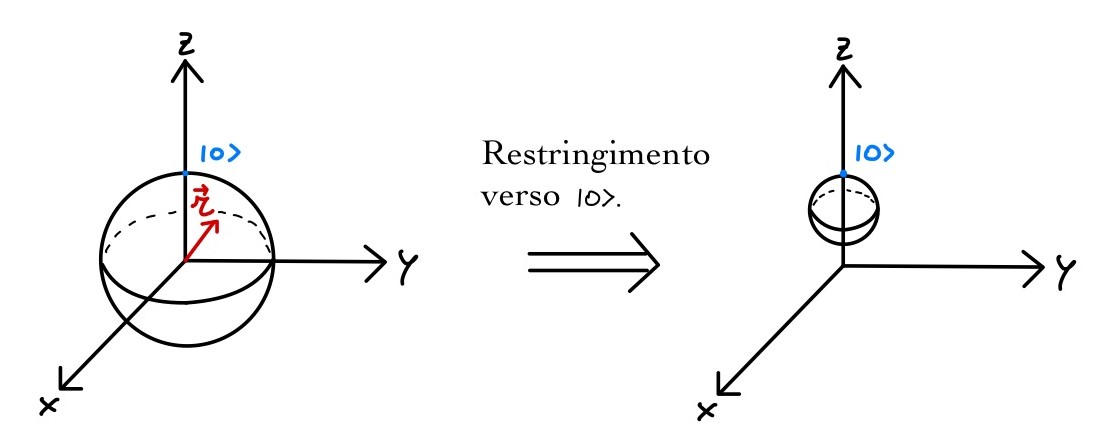
\includegraphics[scale=0.4]{images/shrinking_to_0}
    \caption{La sfera di Bloch si restringe verso lo stato $\ket{0}$ per tempi molto lunghi.}
    \label{fig:shrinking_to_0}
\end{figure}


\subsection{Phase damping}
Un processo di rumore che è unicamente quantistico e descrive la perdita di \textit{coerenza}, ossia di informazioni quantistiche senza perdita di energia, è il \textbf{phase damping} (smorzamento della fase). Fisicamente descrive, ad esempio, cosa succede quando un fotone si disperde casualmente mentre viaggia attraverso una guida d'onda, o come gli stati elettronici in un atomo vengono perturbati quando interagisce con cariche elettriche distanti. Gli autostati energetici di un sistema quantistico non cambiano in funzione del tempo, ma accumulano una fase proporzionale all'autovalore. Quando un sistema evolve per un periodo di tempo non noto con precisione, le informazioni parziali su questa fase relativa, tra gli autostati energetici, vengono perse, quindi questo fenomeno affligge unicamente la fase relativa di una sovrapposizione quantistica di stati. 

\noindent In maniera analoga a quanto visto nell'amplitude damping, possiamo descrivere la fisica dietro al phase damping considerando lo scattering di particelle presenti nell'ambiente con il nostro sistema quantistico. Modelliziamo la situazione dal punto di vista dell'ambiente introducendo la seguente base
\begin{align*}
    \ket{0}_E &= \text{Ground state: nessuno scattering}. \\
    \ket{1}_E &= \text{Scattering che porta al I stato eccitato}. \\
    \ket{2}_E &= \text{Scattering che porta al II stato eccitato},
\end{align*}
dove lo stato eccitato finale dell'ambiente dipender\`a dallo stato del qubit.
In questo modo il sistema totale $\mathcal{H}_q \otimes \mathcal{H}_E$ evolve con l'evoluzione unitaria $U$ tale che
\begin{equation}\label{phase_damping}
    U \, : \; 
    \begin{cases}
        \ket{0} \otimes \ket{0}_E &\rightarrow  \sqrt{1-p} \ket{0} \otimes \ket{0}_E + \sqrt{p} \ket{0} \otimes \ket{1}_E \\
        \ket{1} \otimes \ket{0}_E &\rightarrow  \sqrt{1-p} \ket{1} \otimes \ket{0}_E + \sqrt{p} \ket{1} \otimes \ket{2}_E
    \end{cases} \, ;
\end{equation}
abbiamo indicato con $p$ la probabilità che lo scattering cambi in qualche modo lo stato dell'ambiente: in tutti i casi, trattandosi di scattering, il qubit rimane nel suo stato mentre lo stato che descrive l'ambiente cambia. Come nel caso dell'amplitude damping, l'operatore che descrive le trasformazioni \eqref{phase_damping} è unitario poiché i prodotti scalari sono conservati. L'obiettivo è quello di valutare il nostro sistema (qubit) ignorando l'ambiente e lo facciamo prendendo una traccia della matrice densità $\rho$, ancora una volta, su $\mathcal{H}_E$. Calcoliamo gli operation elements della \eqref{E_k} ricordando, come in precedenza, che $E_k = {}_E \! \mel{k}{U}{0}_E \Leftrightarrow \mel{x}{E_k}{y} = \mel{x k}{U}{y 0}$. In questo caso avremo 3 matrici $E_0$, $E_1$ ed $E_2$:
\begin{align*}
    E_0 &= {}_E \! \mel{0}{U}{0}_E &\Rightarrow& \;
    \begin{cases}
        \mel{0}{E_0}{0}=\mel{00}{U}{00}=\sqrt{1-p} \\
        \mel{1}{E_0}{1}=\mel{10}{U}{10}=\sqrt{1-p} \\
        \mel{0}{E_0}{1}=\mel{00}{U}{10}=0 \\
        \mel{1}{E_0}{0}=\mel{10}{U}{00}=0
    \end{cases} 
    &\Rightarrow&
    &E_0 &= \sqrt{1-p}
          \begin{pmatrix}
            1 & 0 \\
            0 & 1
          \end{pmatrix} \, , \\
    E_1 &= {}_E \! \mel{1}{U}{0}_E &\Rightarrow& \;    \begin{cases}
        \mel{0}{E_0}{0}=\mel{01}{U}{00}=\sqrt{p} \\
        \mel{1}{E_0}{1}=\mel{11}{U}{10}=0 \\
        \mel{0}{E_0}{1}=\mel{01}{U}{10}=0 \\
        \mel{1}{E_0}{0}=\mel{11}{U}{00}=0
    \end{cases}
    &\Rightarrow&
    &E_1 &= \sqrt{p}
          \begin{pmatrix}
            1 & 0 \\
            0 & 0
          \end{pmatrix} \, , \\
    E_2 &= {}_E \! \mel{2}{U}{0}_E &\Rightarrow& \;
    \begin{cases}
        \mel{0}{E_0}{0}=\mel{02}{U}{00}=0 \\
        \mel{1}{E_0}{1}=\mel{12}{U}{10}=\sqrt{p} \\
        \mel{0}{E_0}{1}=\mel{02}{U}{10}=0 \\
        \mel{1}{E_0}{0}=\mel{12}{U}{00}=0
    \end{cases}
    &\Rightarrow&
    &E_2 &= \sqrt{p}
          \begin{pmatrix}
            0 & 0 \\
            0 & 1
          \end{pmatrix} \, .
\end{align*}
Le matrici ottenute soddisfano coerentemente la \eqref{constraint_E_k}:
\begin{align*}
    \sum_k E_k^\dagger E_k &= E_0^\dagger E_0 + E_1^\dagger E_1 +  E_2^\dagger E_2 \\
    &=
    \begin{pmatrix}
        1-p & 0 \\
        0 & 1-p
    \end{pmatrix}
    +
    \begin{pmatrix}
        p & 0 \\
        0 & 0
    \end{pmatrix}
    +
    \begin{pmatrix}
        0 & 0 \\
        0 & p
    \end{pmatrix} = \mathbb{I} \, .
\end{align*}
Avendo ora a disposizione $E_0$, $E_1$ ed $E_2$, possiamo calcolare la \eqref{operator_sum_repr}: 
\begin{align}
    \rho \to \mathcal{E}(\rho) &= \sum_k E_k \rho E_k^\dagger = E_0\rho E_0^\dagger + E_1\rho E_1^\dagger + E_2\rho E_2^\dagger \notag \\
    &= (1-p)\rho + p\frac{\mathbb{I}+\sigma_3}{2}\rho\frac{\mathbb{I}+\sigma_3}{2}+p\frac{\mathbb{I}-\sigma_3}{2}\rho\frac{\mathbb{I}-\sigma_3}{2} \notag \\
    &= (1-p)\rho +\frac 12(p\rho + p\sigma_3\rho \sigma_3) \notag \\
    &= \left( 1-\frac p2 \right) \rho +\frac p2 \sigma_3\rho\sigma_3 \, , \label{matrix_rho_p_damping}
\end{align}
dove nella seconda linea abbiamo utilizzato $E_1 =\sqrt{p} \frac{\mathbb{I}+\sigma_3}{2}$ e $E_2 =\sqrt{p} \frac{\mathbb{I}-\sigma_3}{2}$. Questo risultato non è nient'altro che il conto che avevamo svolto nell'Esempio \ref{es:phase_flip} del phase flip channel. Un altro modo per rendere più esplicito questo fatto è quello di introdurre il cambio di variabili $\tilde{p}=1-\frac p2$ nella precedente
\begin{equation}\label{rho-p-damping}
    \mathcal{E}(\rho) = \tilde{p}\rho+(1-\tilde{p})Z\rho Z \, ,
\end{equation}
e ricordare che \texttt{Z-gate} introduce, in un generico stato, una fase relativa
\begin{equation*}
    \alpha\ket 0+ \beta \ket 1 \overset{Z}{\longrightarrow} \alpha \ket 0 - \beta \ket 1 \, ;
\end{equation*}
(si veda direttamente l'Esempio \ref{es:phase_flip} per capire la trasformazione di $\vec{r}$ e visualizzarne l'effetto sulla sfera di Bloch). Perciò, esplicitando la \eqref{matrix_rho_p_damping}, la generica matrice densità si trasformerà nel seguente modo
\begin{equation*}
    \rho = \begin{pmatrix}
                \rho_{00} & \rho_{01} \\
                \rho_{10} & \rho_{11}
           \end{pmatrix}
    \longrightarrow
    \mathcal{E}(\rho) = \begin{pmatrix}
                            \rho_{00} & (1-p)\rho_{01} \\
                            (1-p)\rho_{10} & \rho_{11}
                        \end{pmatrix} \, ;
\end{equation*}
Ancora una volta, possiamo introdurre un'opportuna ampiezza di scattering $\Gamma$ e sostituire la probabilità con il termine di decadimento esponenziale $(1-p)=e^{-\Gamma t}$ nel limite in cui $n \to \infty$:
\begin{equation}\label{rho_final_phase_damping}
    \mathcal{E}(\rho) = \begin{pmatrix}
                            \rho_{00} & e^{-\Gamma t}\rho_{01} \\
                            e^{-\Gamma t}\rho_{10} & \rho_{11}
                        \end{pmatrix} \, ;
\end{equation}
solamente le componenti off-diagonal risentono dell'interazione con l'ambiente a differenza di quanto avveniva nell'amplitude damping! Ricapitolando: una singola azione del phase flip channel produce una singola aggiunta di una fase, tuttavia molte azioni ripetute dell'ambiente (scattering con le particelle) causano una diminuzione delle componenti off-diagonal di $\rho$, ossia una perdita di coerenza nei termini di interferenza degli stati quantistici.

\noindent Evidenziamo un aspetto particolare che è opportuno menzionare e che incontreremo nuovamente nel capitolo successivo sul \textbf{quantum error-correction}. In questa situazione abbiamo ricavato il risultato \eqref{rho-p-damping} da una prospettiva differente rispetto all'Esempio \ref{es:phase_flip} poiché abbiamo visto che lo stato del qubit può essere modificato a seguito degli scattering con le particelle esterne dell'ambiente. Vi è una sorta di \textbf{universalità}: quando, in fisica, si ritrova un comportamento universale è sempre un fatto positivo, tuttavia è bene ricordare che i qubit, a differenza del CC, sono continui (sovrapposizione di stati, gate unitari dipendenti da parametri continui, ecc.) e quindi sembrerebbe molto difficoltoso controllare tutte le possibili situazioni perché si potrebbe ingenuamente pensare che ci siano un'infinità di errori agenti sui qubit! Il punto fondamentale è che se si aspetta un tempo sufficientemente lungo tutti questi effetti sono indistinguibili e si finisce sempre in una delle due situazioni appena esaminate: si perde energia (amplitude damping) o si perde coerenza (phase damping).

\noindent Storicamente, il phase damping era un processo che è stato quasi sempre pensato, fisicamente, come risultato di un processo casuale di kick di fase o scattering. Non lo è stato fino a quando fu scoperta la connessione al phase flip channel, il quale è stato analizzato nella teoria della correzione degli errori quantistici: si pensava infatti che gli errori di fase fossero continui e non potessero quindi essere descritti come un processo discreto! In effetti, gli errori di fase del singolo qubit possono sempre essere pensati come il risultato di un processo in cui, con probabilità $p$, non accade nulla a un qubit o, con probabilità $1-p$, il qubit viene capovolto dallo \texttt{Z-gate}. Sebbene questo potrebbe non essere l'effettivo processo fisico microscopico che sta accadendo, dal punto di vista della trasformazione che si verifica in un qubit su un intervallo di tempo discreto, ampio rispetto al processo casuale sottostante, non c'è alcuna differenza.

\noindent Vediamo un altro esempio di modello molto semplice che produce il medesimo effetto sul qubit, ossia il phase damping e la conseguente perdita di coerenza. Supponiamo di avere un qubit nello stato $\ket \psi = a \ket 0 + b \ket 1$ che interagisce con l'ambiente, il quale aggiunge al qubit delle fasi casuali in qualche direzione particolare, diciamo una rotazione $R_z(\theta) = e^{-\frac{i \theta \sigma_3}{2}}$ attorno a $z$, dove l'angolo di rotazione $\theta$ è casuale:
\begin{equation}\label{rotation_on_coeffs}
    \ket{\psi} \rightarrow R_z(\theta)\ket \psi = e^{-i\frac \theta 2 \sigma_3}\ket \psi = a e^{-i\frac \theta 2} \ket 0 + b e^{i\frac \theta 2} \ket 1 \, ,
\end{equation}
quindi il suo effetto è quello di frapporre una fase relativa tra $\ket{0}$ e $\ket{1}$. Non vogliamo studiare il caso di un valore particolare di $\theta$, ma vogliamo invece capire che cosa succede quando si hanno errori multipli. Consideriamo un'interazione continua con l'ambiente, il quale causa $\ket{\psi} \to R_z(\theta) \ket{\psi}$ per qualche valore casuale di $\theta$, e supponiamo che l'angolo di rotazione sia una variabile casuale con una ben definita distribuzione di probabilità. Immaginiamo che tale distribuzione sia una gaussiana con media $\theta$ e varianza $2\lambda$: la probabilità di avere un angolo $\theta$ è data da
\begin{equation*}
    P(\theta) = \frac{1}{\sqrt{4 \pi \lambda}} e^{-\frac{\theta^2}{4\lambda}} \, .
\end{equation*}
Vediamo cosa succede al qubit aspettando del tempo: l'effetto di una singola rotazione sullo stato finale del qubit dopo questo processo è descritto dalla seguente matrice densità
\begin{equation*}
    \rho = \op{\psi}{\psi} \rightarrow \mathcal{E}(\rho) =  R_z(\theta)\op{\psi}{\psi}R_z^\dagger(\theta) \, ,
\end{equation*}
quindi se integriamo su tutti i valori di $\theta$ possiamo calcolare un effetto totale mediato
\begin{align*}
    \expval{\mathcal{E}(\rho)}_\theta &= \frac{1}{\sqrt{4\pi\lambda}} \int \dd{\theta} e^{-\frac{\theta^2}{4\lambda}}R_z(\theta)\op{\psi}{\psi}R_z^\dagger(\theta) \\
    &= \frac{1}{\sqrt{4\pi\lambda}} \int \dd{\theta} e^{-\frac{\theta^2}{4\lambda}}R_z(\theta)
    \begin{pmatrix}
        \abs{a}^2 & ab^* \\
        a^*b & \abs{b}^2
    \end{pmatrix}
    R_z^\dagger(\theta) \\
    &= \frac{1}{\sqrt{4\pi\lambda}} \int \dd{\theta} e^{-\frac{\theta^2}{4\lambda}}
    \begin{pmatrix}
        \abs{a}^2 & ab^*e^{-i\theta} \\
        a^*be^{i\theta} & \abs{b}^2
    \end{pmatrix} \, ,
\end{align*}
dove nell'ultima riga abbiamo letto l'effetto di $R_z(\theta)$ su $a$ e $b$ dalla \eqref{rotation_on_coeffs}: $a \to a e^{-i\theta/2}$ e $b \to b e^{i \theta/2}$. L'integrale dei termini diagonali è banale perché cancella esattamente la normalizzazione, mentre l'integrale dei termini off-diagonal è un semplice integrale gaussiano
\begin{equation*}
    \frac{1}{\sqrt{4\pi\lambda}} \int \dd{\theta} e^{-\frac{\theta^2}{4\lambda} \pm i \theta} = \frac{1}{\sqrt{4\pi\lambda}} \int \dd{\theta} e^{-\frac{1}{4\lambda}(\theta \mp 2 \lambda i)^2 - \lambda} = e^{-\lambda} \, ,
\end{equation*}
dove nel penultimo passaggio abbiamo ricostruito il quadrato ad esponente e nell'ultimo abbiamo usato la formula dell'integrale gaussiano. Perciò la matrice densità finale si è modificata in
\begin{equation*}
    \expval{\mathcal{E}(\rho)}_\theta =
    \begin{pmatrix}
        \abs{a}^2 & a b^\ast e^{-\lambda} \\
        a^\ast b e^{-\lambda} & \abs{b}^2
    \end{pmatrix} \, .
\end{equation*}
Ancora una volta abbiamo ottenuto che la media sugli effetti dell'ambiente risulta una soppressione dei termini off-diagonal (legati all'interferenza tra gli stati) per la presenza dei fattori $e^{-\lambda}$. 

\subsection{Combinazione di amplitude e phase damping}
Riassumiamo quanto abbiamo ottenuto per l'\textbf{amplitude damping} e il \textbf{phase damping}. Le matrici densità risultanti sono la \eqref{rho-damping2} e la \eqref{rho_final_phase_damping}:
\begin{align*}
    &\text{Amplitude damping}: &\rho &\rightarrow \mathcal{E}(\rho) =
    \begin{pmatrix}
        \rho_{00}+(1-e^{-\Gamma_a t})\rho_{11} & e^{-\frac{\Gamma_a t}{2}} \rho_{01} \\          e^{-\frac{\Gamma_a t}{2}} \rho_{10} & e^{-\Gamma_a t}\rho_{11}         
    \end{pmatrix} \, , \\
    &\text{Phase damping}: &\rho &\rightarrow \mathcal{E}(\rho) =
    \begin{pmatrix}
        \rho_{00} & e^{-\Gamma_\varphi t}\rho_{01} \\
        e^{-\Gamma_\varphi t}\rho_{10} & \rho_{11}
    \end{pmatrix} \, ,
\end{align*}
dove $\Gamma_a$ è il rateo di decadimento dell'emissione spontanea e $\Gamma_\varphi$ è l'ampiezza di scattering (o equivalentemente la varianza della distribuzione del segnale che causa il rumore). Combinandoli insieme otteniamo
\begin{equation}\label{general-damping}
    \rho =
    \begin{pmatrix}
        \rho_{00} & \rho_{01} \\ \rho_{10} & \rho_{11}
    \end{pmatrix}
    \rightarrow \mathcal{E}(\rho) =
    \begin{pmatrix}
        \rho_{00}+(1-e^{-\Gamma_1 t})\rho_{11} & e^{-\Gamma_2 t}\rho_{01} \\
        e^{-\Gamma_2 t}\rho_{10} & e^{-\Gamma_1 t}\rho_{11}
    \end{pmatrix} \, ,
\end{equation}
dove abbiamo definito
\begin{itemize}
    \item $\Gamma_1=\Gamma_a \equiv \frac 1 {T_1}$;
    \item $\Gamma_2 = \frac {\Gamma_a} 2 + \Gamma_\varphi \equiv \frac 1 {T_2}$.
\end{itemize}
La relazione \eqref{general-damping} descrive in maniera standard ciò che accade alla matrice densità di un qubit a seguito dell'interazione con l'ambiente: gli elementi off-diagonal vengono modificati sia dalla perdita di energia (amplitude damping) sia dalla perdita di coerenza (phase damping) mentre gli elementi sulla diagonale vengono influenzati unicamente dalla perdita di energia attraverso un amplitude damping. Si noti che la \eqref{general-damping} non è data dalla somma dei due effetti (somma di matrici) ma si tratta di una loro opportuna combinazione: spegnendo $\Gamma_\varphi$ riotteniamo la \eqref{rho-damping2}, viceversa sopprimendo $\Gamma_a$ avremo la \eqref{rho_final_phase_damping}. 
    %%%%%%%%%%%%%%
% LECTURE 12 %
%%%%%%%%%%%%%%
\chapter{Quantum error correction}

\lecture{12}{15/11/21}
\vspace{0.5cm}

\noindent Entrambi il CC e il QC sono soggetti ad errori: si pensi ad esempio all'imperfezione dei fili nei circuiti elettrici, ai gate difettosi che non restituiscono il corretto risultato oppure anche al caso dell'interazione con l'ambiente che, come visto nel capitolo precedente, porta sempre ad una perdita di coerenza e di ampiezza nella sovrapposizione quantistica del qubit. A tal proposito, tipicamente il tempo di decoerenza è molto più piccolo rispetto al tempo di decadimento dell'ampiezza, quindi la perdita di interferenza nello stato avviene quasi immediatamente. 

\noindent Nonostante la gestione degli errori di un qubit sia molto più complessa rispetto al caso classico, a causa della continua influenza dell'ambiente, cominciamo la nostra discussione analizzando il caso del CC.

\section{Correzione classica degli errori}\label{sec:classical_correction}
In CC esistono alcuni protocolli standard per affrontare i problemi sopraelencati: il più famoso prevede una \textbf{codifica} del messaggio contenuto nella stringa di bit in esame in una ripetizione di questi ultimi. Questo significa rimpiazzare, ad esempio, $0 \to 000$ e $1 \to 111$: chiaramente la sequenza di 3 bit finali, chiamati \textbf{bit logici}, ha il medesimo significato del bit iniziale (3 bit uguali $=$ 1 bit), tuttavia la differenza è che si hanno molti più bit. 

\noindent A quale vantaggio porta questa sostituzione? Assumendo che gli errori tipici siano equivalenti ad un \texttt{OR} (bit flip: $0 \to 1$ e $1 \to 0$) e che siano statisticamente indipendenti tra loro, allora la probabilità che due o più errori avvengano simultaneamente nella sequenza finale è molto più piccola rispetto ad averne solamente uno: possiamo quindi correggere un qualsiasi errore usando la \textbf{majority rule}. Se la sequenza di bit ricevuti è costituita da $xxx$, allora il ricevente legge "bit inviato $= 0$" se la maggior parte dei bit sono 0, viceversa, quando la maggior parte sono degli 1 allora legge "bit inviato $= 1$". 

\noindent Più formalmente, chiamiamo $p$ la probabilità di avere un singolo bit flip. Quando si codifica il messaggio in un bit singolo si ha probabilità $p$ di avere una qualche sorta di errore, tuttavia se la codifica avviene in 3 bit allora la sicurezza è maggiore. Per vederlo più esplicitamente calcoliamo la probabilità di avere 2 o 3 bit flip contemporaneamente: nel caso di due bit flip avremo $3 p p (1-p) = 3 p^2(1-p)$ (il 3 indica che il primo errore può avvenire in uno dei 3 bit qualsiasi), mentre la probabilità di avere 3 errori è ovviamente $p^3$, dunque la probabilità totale di avere 2 o più errori è data dalla somma $3p^2-2p^3$. Ma si ha
\begin{equation}\label{prob_2_simult}
    3p^2-2p^3 < p \quad \text{per} \quad p < \frac{1}{2} \, ;
\end{equation}
bastano quindi probabilità minori del 50\%, di avere un singolo bit flip, per fare in modo che la probabilità di avere 2 o più errori simultanei sia trascurabile. Codificare il messaggio in 3 bit è più sicuro che lasciare il singolo bit. In generale questo discorso funziona ragionevolmente bene in CC. 

\noindent Analizziamo ora l'analogo quantistico.

\section{Introduzione alla correzione quantistica degli errori}\label{sec:intro_error_corr}
Proviamo a svolgere il medesimo procedimento in QC: rimpiazziamo i singoli qubit con $\ket{0} \to \ket{000}$ e $\ket{1} \to \ket{111}$. Nonostante il problema della duplicazione dei qubit (non è affatto banale raddoppiarli o triplicarli), esistono altri problemi concettuali da tenere necessariamente in considerazione:
\begin{itemize}
    \item[A.] \textbf{Teorema di no-cloning}: non possiamo clonare stati generici. 
    
    \item[B.] \textbf{Errori continui}: in CC tutti gli errori che avvengono sono discreti, ma in QC, dato che i gate dipendono da parametri continui, gli errori possono essere continui (si pensi banalmente all'amplitude e phase damping).
    
    \item[C.] \textbf{Regola di Born}: sappiamo dalla QM che la misurazione porta al collasso della funzione d'onda; per applicare la majority rule sui qubit è quindi necessario interagire con essi e causare irreversibilmente il collasso dello stato.
\end{itemize}

\noindent Nelle prossime sezioni vedremo che tutte queste problematiche possono essere affrontate nella teoria generale della correzione degli errori. 

\noindent Cominciamo ad introdurre il procedimento che si attua per rimpiazzare i qubit iniziali con dei \textbf{qubit logici}. Come prima cosa si vuole rimpiazzare
\begin{align*}
    \ket{0} & \rightarrow \ket{000} \equiv \ket{\overline{0}} \equiv \ket{0}_L \, , \\
    \ket{1} & \rightarrow \ket{111} \equiv \ket{\overline{1}} \equiv \ket{1}_L \, ,
\end{align*}
dove il pedice $L$ sta per "logico". Ricordiamo che un qubit si trova quasi sempre in una sovrapposizione quantistica di stati, quindi si vuole scrivere
\begin{equation}\label{logical_qubit}
    a \ket{0} + b \ket{1} \to a \ket{000} + b \ket{111} \, .
\end{equation}
Possiamo effettuare questa operazione senza violare il punto A.? La risposta è sì ed è quasi banale perché l'operazione precedente non è la stessa che clonare lo stato. Ciò che non è permesso dal \textit{teorema di no-cloning} è \begin{align}\label{forbidden_no_cloning}
    a \ket{0} + b \ket{1} \equiv \ket{\psi} & \rightarrow \ket{\psi} \otimes \ket{\psi} \otimes \ket{\psi} \notag \\
    &= (a \ket{0} + b \ket{1}) \otimes (a \ket{0} + b \ket{1}) \otimes (a \ket{0} + b \ket{1}) \, ;
\end{align} 
chiaramente \eqref{logical_qubit} $\neq$ \eqref{forbidden_no_cloning} perché ciò che vogliamo fare è molto più semplice. 

\noindent Possiamo disegnare un circuito che sia in grado di operare la codifica \eqref{logical_qubit} ricordando che il \texttt{CNOT-gate} inverte lo stato solamente quando il control qubit è in $\ket{1}$:
\begin{center}
    \mbox{
        \Qcircuit @C=2em @R=1em {
            \lstick{a \ket{0} + b \ket{1}} & \ctrl{1} & \ctrl{2} & \qw \\
            \lstick{\ket{0}} & \targ & \qw & \qw \\
            \lstick{\ket{0}} & \qw & \targ & \qw
        }
    }
\end{center}
è chiaro vedere che quando il primo qubit è in $\ket{0}$ allora si ottiene $\ket{000}$ e viceversa quando è in $\ket{1}$ i due \texttt{CNOT-gate} agiscono e producono $\ket{111}$. Questo circuito non contraddice il teorema di no-cloning: ad esempio se il primo qubit si trova in $\ket{1}$ allora il circuito avrà come output
\begin{equation*}
    b \ket{1} \otimes \ket{0} \otimes \ket{0} \to b \ket{1} \otimes \ket{1} \otimes \ket{1} \, ,
\end{equation*}
il quale è effettivamente il risultato di una clonazione perché se chiamiamo $\ket{1} \equiv \ket{\psi}$ allora l'operazione è
\begin{equation*}
    \ket{\psi} \otimes \ket{0} \otimes \ket{0} \to  \ket{\psi} \otimes \ket{\psi} \otimes \ket{\psi} \, ;
\end{equation*}
nonostante ciò, la dimostrazione del teorema di no-cloning falliva per stati ortogonali, il che significa che non c'è contraddizione fisica nel clonare stati appartenenti ad una base. Il teorema non è violato perché lo stato clonato non è uno stato generico. 

\noindent Vogliamo cercare di capire come rilevare possibili errori. Supponiamo che si possano verificare errori di bit flip: gli errori causano $\ket{0} \to \ket{1}$ e $\ket{1} \to \ket{0}$ e questa operazione può essere implementata in un circuito con un \texttt{X-gate}. Immaginiamo che il circuito precedente sia soggetto ad un errore di questo tipo: 
\begin{center}
    \mbox{
        \Qcircuit @C=2em @R=1em {
            \lstick{} & \ctrl{1} & \ctrl{2} & \gate{X} & \qw \\
            \lstick{} & \targ & \qw & \qw & \qw \\
            \lstick{} & \qw & \targ & \qw & \qw
            \gategroup{1}{4}{1}{4}{.7em}{--}
        }
    }
\end{center}
(il gate è stato inserito nel primo qubit, ma il discorso è analogo anche se fosse stato nel secondo o terzo). Il nostro scopo è quello di correggere l'errore tratteggiato senza disturbare in maniera eccessiva il sistema. Chiaramente essendo l'output il seguente
\begin{equation*}
    a \ket{000} + b \ket{111} \overset{X}{\longrightarrow} a \ket{100} + b \ket{011} \, ,
\end{equation*}
dobbiamo cercare di capire come rilevare questo errore senza causare il collasso dello stato e come intervenire per ripristinare l'informazione desiderata. 

\noindent Vediamo questo errore in generale. Se solamente singoli\footnote{Stiamo assumendo che la probabilità che avvengano 2 o più errori simultaneamente è soppressa rispetto alla probabilità che avvenga un singolo bit flip. Si veda l'equazione \eqref{prob_2_simult} per ulteriori dettagli.} \texttt{X-gate} su singoli qubit possono intervenire allora, a seconda della posizione di questo gate in uno dei 3 qubit, possono verificarsi 4 casi (compresa la situazione in cui non avviene alcun errore):
\begin{equation}\label{distinguish_cases}
    a \ket{000} + b \ket{111} \rightarrow
    \begin{cases}
    a \ket{000} + b \ket{111} \, , &\text{Caso I} \\
    a \ket{100} + b \ket{011} \, , &\text{Caso II} \\
    a \ket{010} + b \ket{101} \, , &\text{Caso III} \\
    a \ket{001} + b \ket{110} \, , &\text{Caso IV}
    \end{cases} \, .
\end{equation}
Come possiamo distinguere in quale dei 4 casi ci troviamo? Possiamo pensare di costruire un circuito che distingua le situazioni senza disturbare i 3 qubit in gioco. Per farlo aggiungiamo, dopo i due \texttt{CNOT-gate} che servono per produrre \eqref{logical_qubit}, due qubit extra, chiamati \textbf{ancilla qubit}\footnote{Il nome "ancilla" deriva dal latino \textit{ancilla}, che significa "ancella", "serva", "schiava". Sì, sono qubit schiavi.}, e costruiamo il seguente circuito:
\begin{center}
    \mbox{
        \Qcircuit @C=2em @R=1em {
            \lstick{} & \targ & \targ & \qw & \qw & \meter & \rstick{\ket{x} = \ket{0}, \ket{1}} \qw \\
            \lstick{\raisebox{2.8em}{$\large{\substack{\text{Ancilla qubit} \\ \text{preparati in } \ket{0}}}$ \ }} & \qw & \qw & \targ & \targ & \meter & \rstick{\ket{y} = \ket{0}, \ket{1}} \qw \gategroup{1}{1}{2}{1}{1.2em}{\{} \\
            \lstick{} & \ctrl{-2} & \qw & \qw & \qw & \qw & \qw \\
            \lstick{} & \qw & \ctrl{-3} & \ctrl{-2} & \qw & \qw & \qw \\
            \lstick{\raisebox{2.8em}{$\large{\substack{\text{Qubit dei casi} \\ \text{I, II, III e IV}}}$}\ \ } & \qw & \qw & \qw & \ctrl{-3} & \qw & \qw \gategroup{3}{1}{5}{1}{1em}{\{}
        }
    }
\end{center}
In questo circuito i 3 qubit in esame agiscono sempre da control qubit, quindi rimangono tali non essendo soggetti ad alcun flip dovuto ai diversi \texttt{CNOT-gate} (questo significa che il punto C. è rispettato). Come indicato, si svolge una misurazione sugli ancilla qubit: il risultato, che non causa alcun collasso dei 3 qubit in esame, è un insieme di due numeri $(x,y)$ che possono essere utilizzati per distinguere quale dei 4 errori è avvenuto. Tenendo presente gli stati indicati in \eqref{distinguish_cases} nei differenti casi, avremo le seguenti situazioni:
\begin{enumerate}
    \item \textbf{Caso I}: $(x,y) = (0,0)$.
    
    \noindent La parte che riguarda $\ket{000}$ non produce alcuna modifica perché i 4 \texttt{CNOT-gate} non agiscono; la parte di $\ket{111}$, invece, attiva tutti e 4 i \texttt{CNOT-gate} ma non produce alcuna variazione finale degli stati $\ket{x} = \ket{0}$ e $\ket{y} = \ket{0}$ perché si hanno due flip consecutivi. 
    
    \item \textbf{Caso II}: $(x,y) = (1,0)$.
    
    \noindent Lo stato $\ket{100}$ attiva solamente il primo \texttt{CNOT-gate} sul primo ancilla; lo stato $\ket{011}$ attiva gli altri 3, di cui uno sul primo ancilla (come in precedenza) e due consecutivi sul secondo ancilla. Il risultato è quindi $\ket{x} = \ket{1}$ e $\ket{y} = \ket{0}$ per entrambi. 
    
    \item \textbf{Caso III}: $(x,y) = (1,1)$. 
    
    \noindent Lo stato $\ket{010}$ attiva i due \texttt{CNOT-gate} centrali che agiscono sui due diversi ancilla; lo stato $\ket{101}$ attiva il primo e il quarto \texttt{CNOT-gate}, che anch'essi agiscono su due diversi ancilla. In entrambi i casi si ha un flip su ogni stato e quindi avremo $\ket{x} = \ket{1}$ e $\ket{y} = \ket{1}$. 
    
    \item \textbf{Caso IV}: $(x,y) = (0,1)$.
    
    \noindent Lo stato $\ket{001}$ attiva solamente l'ultimo \texttt{CNOT-gate}, che modifica il secondo ancilla; lo stato $\ket{110}$ attiva i primi 3 \texttt{CNOT-gate}: i primi due non producono alcuna differenza sul primo ancilla, mentre il terzo inverte il secondo ancilla. Il risultato per entrambe le situazioni è quindi $\ket{x} = \ket{0}$ e $\ket{y} = \ket{1}$. 
\end{enumerate}

\noindent Una volta effettuata la misurazione sugli ancilla e distinto il caso in esame, si può facilmente intervenire sul qubit corrotto inserendo un \texttt{X-gate} che lo riporti alla situazione iniziale. Si noti, ancora una volta, che non si è misurato il qubit difettoso, ma si sa della sua presenza grazie al risultato degli ancilla. In generale, al posto che effettuare le misure sugli ancilla, è possibile implementare un circuito che svolga questo lavoro in automatico (compreso l'inserimento dell'\texttt{X-gate} per correggere il qubit). 

\section{Stabilizers}\label{sec:stabilizers}
Qual è il significato fisico in termini di osservabili della misurazione $(x,y)$ che viene effettuata sugli ancilla qubit? 

\noindent Prima di rispondere a questa domanda fissiamo le notazioni: i 3 qubit soggetti ad errori vengono generalmente indicati con un numero, come ad esempio
\begin{center}
    \mbox{
        \Qcircuit @C=2em @R=1em {
            \lstick{0} & \gate{X} & \qw \\
            \lstick{1} & \qw & \qw \\
            \lstick{2} & \qw & \qw 
        }
    }
\end{center}
\vspace{0.2cm}
L'\texttt{X-gate} mostrato, invece, corrisponde, in termini di operatori agenti sui 3 qubit, al prodotto tensoriale $X_0 \otimes \mathbb{I}_1 \otimes \mathbb{I}_2$. Per semplicità scriveremo sempre $X_0 \otimes \mathbb{I}_1 \otimes \mathbb{I}_2 \equiv X_0$, $\mathbb{I}_0 \otimes X_1 \otimes \mathbb{I}_2 \equiv X_1$ e così via: i pedici sugli operatori indicano il qubit su cui esso sta agendo. 

\noindent Lo spazio di Hilbert dei 3 qubit, che indicheremo con $\mathcal{H}$, ha dimensione $\dim \mathcal{H} = 2^3 = 8$ perché i qubit logici che stiamo considerando sono triplette dei qubit singoli iniziali: $\ket{\overline{0}} = \ket{000}$ e $\ket{\overline{1}} = \ket{111}$. Chiamiamo \textbf{codewords} gli stati del seguente sottospazio
\begin{equation}\label{codewords}
    C = \left\lbrace \ket{\psi} \in \mathcal{H} \; : \; \ket{\psi} = a \ket{000} + b \ket{111} \right\rbrace \subset \mathcal{H} \, ,
\end{equation}
ossia l'insieme di tutti i vettori di $\mathcal{H}$ che si scrivono come in \eqref{logical_qubit}. Gli operatori che agiscono su $\mathcal{H}$ che ci interessano particolarmente  sono della forma $M = M_0 \otimes M_1 \otimes M_2$ dove $M_i = \{ \mathbb{I}, X, Y, Z \}$. Questi operatori $M$ sono molto speciali perché sono fattorizzati come prodotto di matrici: non stiamo agendo su $\ket{\overline{0}}$ e $\ket{\overline{1}}$ con generiche matrici $8 \times 8$; in aggiunta, se consideriamo le singole matrici $M_i$ $2 \times 2$ che agiscono sui singoli qubit esse non sono matrici generali di $U(2)$. Alcuni semplici esempi di operatori $M$ sono: $X \otimes \mathbb{I} \otimes \mathbb{I}$, $X \otimes Z \otimes \mathbb{I}$ e $Y \otimes Z \otimes X$.

\noindent Perché questi operatori sono così importanti? In primo luogo perché grazie alla proprietà $\sigma_i^2 = \mathbb{I}$ allora $M^2 = \mathbb{I}$. Ad esempio se $M = X \otimes Z \otimes \mathbb{I}$ avremo
\begin{equation*}
    M^2 = (X \otimes Z \otimes \mathbb{I}) (X \otimes Z \otimes \mathbb{I}) = X^2 \otimes Z^2 \otimes \mathbb{I}^2 = \mathbb{I} \otimes \mathbb{I} \otimes \mathbb{I} \equiv \mathbb{I} \, .
\end{equation*}
In secondo luogo, le matrici di Pauli sono hermitiane, il che vuol dire che possono essere diagonalizzate. I possibili autovalori ($\lambda = \pm 1$) e autovettori delle matrici di Pauli sono mostrati nella Tabella \ref{tab:Pauli_eig} della Sezione \ref{sec:osservabili}. 

\noindent Grazie alla due ragioni precedenti vale il seguente risultato: se $M$ è non banale (almeno una $M_i \neq \mathbb{I}$) allora lo spazio di Hilbert dei qubit può essere decomposto come somma diretta di due sottospazi della medesima dimensione corrispondenti agli autovalori $\lambda = \pm 1$ dell'operatore $M$ (autospazi di $M$). In termini matematici possiamo scrivere 
\begin{equation}\label{decomposition_direct_sum}
    \mathcal{H} = \mathcal{H}_1 \oplus \mathcal{H}_2 \, , \quad \text{con} \quad \dim \mathcal{H}_1 = \dim \mathcal{H}_2 \, ;
\end{equation}
questo significa quindi che $\mathcal{H}$ è "tagliato" da $M$ in due sottospazi della stessa dimensione. Cerchiamo di capirlo meglio con un esempio:

\begin{esempio}\label{es:M}
    Supponiamo che l'operatore sia $M = X \otimes \mathbb{I} \otimes \mathbb{I}$. Dato che abbiamo la matrice $\sigma_x$ è meglio utilizzare la base composta dai suoi autostati: si ha $X \ket{\pm} = \pm \ket{\pm}$, quindi la tripletta di qubit è costituita dagli stati della forma $\{ \ket{\pm \pm \pm} \}$. Lo spazio di Hilbert totale è tagliato negli autospazi:
    \begin{equation}\label{H_1_H_2}
        \mathcal{H}_1 = \{ \ket{+ \pm \pm} \} \, , \qquad \mathcal{H}_2 = \{ \ket{- \pm \pm} \} \, ,
    \end{equation}
    dove entrambi gli spazi hanno dimensione 4 poiché sono costituiti da 4 stati differenti. Tutti gli stati di $\mathcal{H}_1$ sono autostati di $M$ con autovalore 1 e similmente tutti gli stati di $\mathcal{H}_2$ sono autostati di $M$ con autovalore $-1$.  
\end{esempio}

\noindent Il fatto che valga la \eqref{decomposition_direct_sum} non è una coincidenza perché per ogni operatore $M$ non banale esiste un operatore invertibile $S$ tale che $S \; : \; \mathcal{H}_1 \to \mathcal{H}_2$ (i due sottospazi $\mathcal{H}_1$ e $\mathcal{H}_2$ sono infatti isomorfi perché possiamo sempre tornare indietro). 

\begin{esempio}
    In riferimento all'Esempio \ref{es:M}, possiamo scegliere una matrice che anticommuta con $X$, come $Z$ ad esempio, e scrivere $S = Z \otimes \mathbb{I} \otimes \mathbb{I}$. Come agisce $Z$ su $\ket{\pm}$? Ricordiamo che
    \begin{equation*}
        Z \ket{\pm} = Z \frac{\ket{0} \pm \ket{1}}{\sqrt{2}} = \frac{\ket{0} \mp \ket{1}}{\sqrt{2}} = \ket{\mp} \, ;
    \end{equation*}
    in riferimento ai sottospazi in \eqref{H_1_H_2}, è evidente che se partiamo da $\ket{\psi_1} \in \mathcal{H}_1$ allora $S \ket{\psi_1} = \ket{- \pm \pm} \equiv \ket{\psi_2} \in \mathcal{H}_2$. Chiaramente è invertibile perché basta applicare nuovamente $S$ a $\ket{\psi_2}$ per ottenere uno stato di $\mathcal{H}_1$. 
\end{esempio}

\noindent L'esempio precedente funzionava perché l'operatore scelto anticommutava con $M$: se possiamo trovare un operatore $S$ tale che $\acomm{S}{M} = 0$ allora tale operatore agisce come $S \; : \; \mathcal{H}_1 \to \mathcal{H}_2$ per una ragione algebrica molto semplice. Consideriamo uno stato $\ket{\psi_1} \in \mathcal{H}_1$, quindi $M \ket{\psi_1} = \ket{\psi_1}$ perché $\mathcal{H}_1$ è autospazio di $M$ con autovalore associato $\lambda = +1$. Allora
\begin{equation*}
    M \left( S \ket{\psi_1} \right) = - S \left( M \ket{\psi_1} \right) = - S \ket{\psi_1} \, ,
\end{equation*}
quindi $S \ket{\psi_1}$ è autovettore di $M$ con autovalore associato $\lambda = -1$: questo significa necessariamente che $S \ket{\psi_1} \in \mathcal{H}_2$.

\noindent Dopo questa digressione matematica ritorniamo al nostro problema originale nel capire qual è il significato fisico delle misure effettuate sugli ancilla qubit. Cosa c'è di speciale negli stati che si scrivono come in \eqref{codewords}? Possiamo identificarli in qualche modo? Definiamo gli operatori
\begin{align*}
    Z_0 Z_1 &= Z \otimes Z \otimes \mathbb{I} \, , \\
    Z_1 Z_2 &= \mathbb{I} \otimes Z \otimes Z \, ,
\end{align*}
dove i pedici indicano su quali qubit le matrici $Z$ stanno agendo. Tutti gli stati di $C$ in \eqref{codewords} sono autostati di questi due operatori con autovalori $+1$ per entrambi: questo è ovvio perché $Z \ket{0} = \ket{0}$ e $Z \ket{1} = - \ket{1}$, infatti
\begin{align*}
    Z_0 Z_1 \ket{000} &= \ket{000} \, , & Z_1 Z_2 \ket{000} &= \ket{000} \, , \\
    Z_0 Z_1 \ket{111} &= \ket{111} \, , & Z_1 Z_2 \ket{111} &= \ket{111} \, .
\end{align*}

\noindent Affermiamo inoltre che gli stati di $C$ sono il più generale autovettore comune di $Z_0 Z_1$ e $Z_1 Z_2$. La ragione è la seguente: entrambi gli operatori sono della forma di $M$ e ognuno dei due, come autospazio, taglia lo spazio di Hilbert totale $\mathcal{H}$ in 2 sottospazi, le cui dimensioni sono la metà della dimensione dello spazio di partenza (ossia 4). Entrambi gli operatori $Z_0 Z_1$ e $Z_1 Z_2$ possono avere autovalori $\pm 1$: focalizzandoci sull'autovalore in comune, ossia $+1$, abbiamo che la dimensionalità viene tagliata in $8/2/2 = 2$, dove il primo taglio è operato da $Z_0 Z_1$ e il secondo da $Z_1 Z_2$. La dimensionalità rimanente, ossia 2, indica che l'autospazio comune agli operatori ha dimensione 2, e infatti $C$ ha proprio dimensione 2 (tutti gli stati della \eqref{codewords} dipendono da due coefficienti generici, quindi $\dim C = 2$). 

\noindent Alla luce di questo discorso affermiamo che le misure sugli ancilla qubit sono legate agli autovalori $x$ di $Z_0 Z_1$ e $y$ di $Z_1 Z_2$. Gli autovalori dell'azione di questi operatori sugli stati della \eqref{distinguish_cases} sono mostrati nella Tabella \ref{tab:eigs_ZZ}. Si noti che ciascun caso è un sottospazio di $\mathcal{H}$ di dimensione 2 (gli stati dipendono da due coefficienti generici) quindi riempiono tutto lo spazio di Hilbert totale ($8 = 2 + 2 + 2 +2$). 
Gli autovalori di questi operatori permettono di distinguere i 4 differenti autospazi, ossia le 4 differenti situazioni (qubit intatto o qubit corrotto da uno dei 3 errori).

\begin{table}[!ht]
	\centering
    \begin{tabular}{llcc}
        \toprule
        Caso & Autospazio & Autovalore di $Z_0 Z_1$ & Autovalore di $Z_1 Z_2$ \\
        \midrule
        I & $C = \{ a \ket{000} + b \ket{111} \}$ & $+1$ ($x=0$) & $+1$ ($y=0$) \\
        II & $E_{II} = \{ a' \ket{100} + b' \ket{011} \}$ & $-1$ ($x=1$) & $+1$ ($y=0$) \\
        III & $E_{III} = \{ a'' \ket{010} + b'' \ket{101} \}$ & $-1$ ($x=1$) & $-1$ ($y=1$) \\
        IV & $E_{IV} = \{ a''' \ket{001} + b''' \ket{110} \}$ & $+1$ ($x=0$) & $-1$ ($y=1$) \\
        \bottomrule
    \end{tabular}\\
    \caption{Autovalori degli operatori $Z_0 Z_1$ e $Z_1 Z_2$ sugli autospazi delle differenti situazioni in \eqref{distinguish_cases}. Se associamo agli autovalori le misure $(\lambda = +1) \to (x, y = 0)$ e $(\lambda = -1) \to (x,y = 1)$ allora questi autovalori permettono di distinguere i 4 differenti autospazi perché i valori corrispondenti di $(x,y)$ sono esattamente le misurazioni effettuate sugli ancilla qubit.}
    \label{tab:eigs_ZZ}
\end{table}

\noindent Abbiamo detto che un errore non è altro che un \texttt{X-gate} agente su un qubit: dato che $\acomm{X}{Z} = 0$ allora, come evidenzia anche la Tabella \ref{tab:acomm_ZZ}, le misure sugli ancilla qubit non sono altro che i segni rimanenti nelle anticommutazioni di $X_i$ con gli operatori $Z_0 Z_1$ e $Z_1 Z_2$. Esplicitamente avremo:
\begin{align*}
    (Z_0 Z_1) \mathbb{I} &= \mathbb{I} (Z_0 Z_1) \, , &(Z_1 Z_2) \mathbb{I} &= \mathbb{I} (Z_1 Z_2) \, , \\
    (Z_0 Z_1) X_0 &= - X_0 (Z_0 Z_1) \, , &(Z_1 Z_2) X_0 &= X_0 (Z_1 Z_2) \, , \\
    (Z_0 Z_1) X_1 &= - X_1 (Z_0 Z_1) \, , &(Z_1 Z_2) X_1 &= - X_1 (Z_1 Z_2) \, , \\
    (Z_0 Z_1) X_2 &= X_2 (Z_0 Z_1) \, , &(Z_1 Z_2) X_2 &= - X_2 (Z_1 Z_2) \, .
\end{align*}
Si noti che un determinato $X_i$ commuta sempre con le matrici appartenenti ad un differente sottospazio (differente qubit).

\begin{table}[!hb]
	\centering
    \begin{tabular}{c|cccc}
        \toprule
        Operatore & Segno $\mathbb{I}$ & Segno $X_0$ & Segno $X_1$ & Segno $X_2$ \\
        \midrule
        $Z_0 Z_1$ & $+1$ ($x = 0$) & $-1$ ($x = 1$) & $-1$ ($x = 1$) & $+1$ ($x = 0$) \\
        $Z_1 Z_2$ & $+1$ ($y = 0$) & $+1$ ($y = 0$) & $-1$ ($y = 1$) & $-1$ ($y = 1$) \\
        \bottomrule
    \end{tabular}\\
    \caption{Il segno rimanente dell'anticommutazione degli operatori $X_i$ (gli \texttt{X-gate} che implementano l'errore) con gli operatori $Z_0 Z_1$ e $Z_1 Z_2$ è esattamente la misura (mostrata tra parentesi) che viene effettuata sui due ancilla qubit.}
    \label{tab:acomm_ZZ}
\end{table}

\noindent Questo formalismo che abbiamo utilizzato per rilevare gli errori è spesso chiamato \textbf{syndrome error correction}. In generale il prodotto delle matrici di Pauli in questi operatori è molto utile per scrivere degli algoritmi per la rilevazione di errori: codici basati su questa logica vengono detti \textbf{stabilizer codes}; gli operatori $Z_0 Z_1$ e $Z_1 Z_2$ sono detti \textbf{stabilizers}. Nelle sezioni successive vedremo alcuni di questi codici famosi.

\noindent Abbiamo detto che lo spazio di Hilbert totale dei 3 qubit può essere visto come somma dei sottospazi $C$, $E_{II}$, $E_{III}$ e $E_{IV}$ perché ciascuno ha dimensione 2, quindi $2^3 = 8$ è scrivibile come $2 + 2 + 2 + 2$. Gli spazi degli errori sono 3 poiché stiamo studiando solamente i bit flip errors, i quali possono accadere in 3 posizioni differenti dei qubit logici. La domanda è: avremmo potuto fare di meglio se avessimo scelto di codificare il messaggio in un numero maggiore di qubit? Se si vuole correggere gli errori di bit flip codificando 1 qubit in $n$ qubit, qual è il minimo valore di $n$ da utilizzare? Per rispondere a queste domande ripartiamo dalla \eqref{codewords}: sappiamo che $C$ ha dimensione 2 e immaginiamo che codifichi i singoli qubit di partenza in $n$ qubit logici, che chiamiamo $\ket{\overline{0}}$ e $\ket{\overline{1}}$; per ognuno di essi è possibile il verificarsi di un errore e in tal caso si necessita uno "spazio dell'errore" ortogonale\footnote{Se lo spazio è ortogonale a tutti gli altri allora la misurazione non influenza in alcun modo gli altri spazi.} a tutti gli altri. Il numero degli spazi necessari sarà quindi $ 2 + 2n$: il primo termine è la dimensione del codewords mentre il secondo è la dimensione del numero di spazi necessari per correggere $n$ qubit\footnote{Il $2$ deriva dal fatto che si debbano correggere entrambi i qubit logici $\ket{\overline{0}}$ e $\ket{\overline{1}}$, mentre il fattore $n$ indica che l'errore si può trovare in uno degli $n$ qubit di quello logico. Ad esempio per $n=4$ si avrà $\ket{\overline{0}} = \ket{0000}$ e $\ket{\overline{1}} = \ket{1111}$: vanno corretti entrambi i qubit logici e in più l'errore si può trovare in ciascuno dei quattro "posti" nel ket di stato.}. Dato che la dimensione dello spazio di Hilbert di $n$ qubit è $2^n$, allora per avere un codewords e degli spazi degli errori mutualmente ortogonali dovremo avere
\begin{equation*}
    2^n \geq 2 + 2 n \, , \quad \Rightarrow \quad 2^{n-1} \geq 1 + n \, .
\end{equation*}
Il minimo numero che soddisfa la disuguaglianza precedente è proprio $n = 3$.

\noindent Il \textbf{bit flip error} appena analizzato non è l'unico errore che si può verificare: talvolta può accadere ad esempio un \textbf{phase flip error}, il quale è facilmente implementabile nei circuiti con un semplice \texttt{Z-gate} ricordando che $Z \ket{0} = \ket{0}$ e $Z \ket{1} = -\ket{1}$. Per analizzare una situazione di questo tipo bisogna ricordarsi che per cambiare base da quella di $Z$, $\{ \ket{0}, \ket{1} \}$, a quella di $X$, $\{ \ket{+}, \ket{-} \}$, basta applicare un \texttt{H-gate} (si ricordi la matrice \eqref{Hadamard_matrix}): $H \ket{0} = \ket{+}$ e $H \ket{1} = \ket{-}$. 

\noindent Per correggere gli errori di phase flip è quindi necessario codificare gli stati in maniera differente: $\ket{0} \to \ket{+++}$ e $\ket{1} \to \ket{---}$. Se si parte con uno stato generico $a \ket{+++} + b \ket{---}$ allora l'azione dello \texttt{Z-gate} è semplicemente quella di scambiare $+ \leftrightarrow -$:
\begin{align*}
    a \ket{+++} + b \ket{---} &\overset{Z_0}{\longrightarrow} a \ket{-++} + b \ket{+--} \, , \\
    a \ket{+++} + b \ket{---} &\overset{Z_1}{\longrightarrow} a \ket{+-+} + b \ket{-+-} \, , \\
    a \ket{+++} + b \ket{---} &\overset{Z_2}{\longrightarrow} a \ket{++-} + b \ket{--+} \, .
\end{align*}
A questo punto la logica è esattamente la stessa di quella che abbiamo adoperato in precedenza! In termini di circuiti, per costruire una tale codifica è necessario aggiungere 3 \texttt{H-gate} al termine del circuito originale:
\begin{center}
    \mbox{
        \Qcircuit @C=2em @R=1em {
            \lstick{a \ket{0} + b \ket{1}} & \ctrl{1} & \ctrl{2} & \gate{H} & \qw \\
            \lstick{\ket{0}} & \targ & \qw & \gate{H} & \qw \\
            \lstick{\ket{0}} & \qw & \targ & \gate{H} & \qw
        }
    }
\end{center}
Infatti dopo i due \texttt{CNOT-gate} lo stato è come in \eqref{logical_qubit}, mentre dopo i 3 \texttt{H-gate} si avrà 
\begin{equation}\label{eig_X_1}
    a \ket{000} + b \ket{111} \overset{H^{\otimes 3}}{\longrightarrow} a \ket{+++} + b \ket{---} \, .
\end{equation}
Da qui in poi per correggere gli errori si agisce esattamente come prima: questa volta lo stato \eqref{eig_X_1} è autostato degli operatori $X_0 X_1$ e $X_1 X_2$ con autovalore $+1$ e ogni qualvolta avverrà un phase flip error si potrà rilevare l'errore per mezzo del cambiamento di tale autovalore. La discussione è identica alla precedente sostituendo $Z \leftrightarrow X$, $\ket{0} \leftrightarrow \ket{+}$ e $\ket{1} \leftrightarrow \ket{-}$: si tratta solamente di un cambio di base!

\noindent Chiaramente può sorgere spontanea la domanda: come faccio se voglio correggere entrambi i bit-phase flip errors? Nelle prossime sezioni vedremo che il codice che si utilizza, dovuto nuovamente a Shor, utilizza solamente 9 qubit per correggere qualsiasi tipologia di errore (assicurando in questo modo che anche il problema B. di inizio sezione sia risolto). Vedremo che correggere tutti gli errori riguardanti i gate $X,Y,Z$ è equivalente a correggere qualsiasi tipologia di errore continuo!


    %%%%%%%%%%%%%%
% LECTURE 13 %
%%%%%%%%%%%%%%
\vspace{1cm}
\noindent \lecture{13}{19/11/21}

\section{Codice di correzione di Shor a 9 qubit}
Nel 1995 Peter Shor propose il primo codice di correzione degli errori quantistici in grado di correggere errori arbitrari a singolo qubit. La sua proposta, in breve, consisteva in una concatenazione dei circuiti di bit flip error e phase flip error che abbiamo visto nelle sezioni precedenti. Per il primo livello di codifica, si garantisce la protezione dagli errori legati al phase flip codificando i qubit logici $\ket{\overline 0}$ e $\ket{\overline 1}$ utilizzando il codice di phase flip a 3 qubit:
\begin{equation}\label{qe-shor1}
    \ket{\overline 0} \rightarrow \ket{+++} \, , \qquad \qquad \ket{\overline 1} \rightarrow \ket{---} \, .
\end{equation}
Come abbiamo notato sopra, tuttavia, questa codifica è suscettibile a errori di bit flip. Per proteggerci da questo tipo di errori prendiamo ciascuno degli stati $\ket +$ e $\ket -$ e, ricordando le \eqref{basi_di_sigma_12}, codifichiamo ciascun $\ket{0}$ e $\ket{1}$ utilizzando il codice di bit flip a 3 qubit. In questo modo la codifica finale è costituita da 9 qubit in totale:
\begin{align}
    &\ket{+++} \rightarrow \frac{\ket{000}+\ket{111}}{\sqrt 2}\frac{\ket{000}+\ket{111}}{\sqrt 2}\frac{\ket{000}+\ket{111}}{\sqrt 2} \equiv \ket{\overline{0}} \, , \label{qe-shor2} \\
    &\ket{---} \rightarrow \frac{\ket{000}-\ket{111}}{\sqrt 2}\frac{\ket{000}-\ket{111}}{\sqrt 2}\frac{\ket{000}-\ket{111}}{\sqrt 2} \equiv \ket{\overline{1}} \, . \label{qe-shor3}
\end{align}
Mettendo insieme i due passaggi che coinvolgono prima la correzione di eventuali phase flip in \eqref{qe-shor1} e dopo la correzione di eventuali bit flip in \eqref{qe-shor2} e \eqref{qe-shor3} avremo quindi la codifica
\begin{equation*}
    \ket{\overline 0} = \left(\frac{\ket{000}+\ket{111}}{\sqrt 2}\right)^{\otimes 3} \, , \qquad \qquad \ket{\overline 1} = \left(\frac{\ket{000}-\ket{111}}{\sqrt 2}\right)^{\otimes 3} \, .
\end{equation*}
Questi passaggi possono essere implementati nel circuito seguente
\begin{center}
    \mbox{
        \Qcircuit @C=1em @R=0.1 em {
            & \qw & \ctrl{3} & \ctrl{6} & \gate{H} & \qw & \ctrl{1} & \ctrl{2} & \qw \gategroup{1}{6}{3}{9}{.7em}{--} \\
            &     &          &          &          &     & \targ    & \qw      & \qw \\
            &     &          &          &          &     & \qw      & \targ    & \qw \\
            & \qw & \targ    & \qw      & \gate{H} & \qw & \ctrl{1} & \ctrl{2} & \qw 
            \gategroup{4}{6}{6}{9}{.7em}{--} \\
            &     &          &          &          &     & \targ    & \qw      & \qw \\
            &     &          &          &          &     & \qw      & \targ    & \qw \\
            & \qw & \qw      & \targ    & \gate{H} & \qw & \ctrl{1} & \ctrl{2} & \qw \gategroup{7}{6}{9}{9}{.7em}{--} \\
            &     &          &          &          &     & \targ    & \qw      & \qw \\
            &     &          &          &          &     & \qw      & \targ    & \qw
        }
    }
\end{center}
Come sopra descritto, la prima parte del circuito (fino a dopo gli \texttt{H-gate}) codifica il qubit utilizzando il codice relativo al phase flip a tre qubit. La seconda parte del circuito codifica ciascuno di questi tre qubit mediante il codice relativo al bit flip; in particolare fa uso di tre copie del circuito di codifica bit flip (si vedano le 3 subroutine tratteggiate). Questo metodo di codifica che utilizza una gerarchia di livelli è noto come \textit{concatenazione}. 

\noindent Per capire se il codice di Shor sia effettivamente in grado di proteggere da errori di phase flip e bit flip su qualsiasi qubit dobbiamo trovare un insieme di operatori tali che $\ket{\overline{0}}$ e $\ket{\overline{1}}$ siano autostati col medesimo autovalore. Per capire la logica generale di funzionamento facciamo un semplice esempio. 

\begin{esempio}
    Supponiamo che si verifichi un bit flip sul primo qubit (blocco I). Per quanto riguarda il codice relativo al bit flip, possiamo eseguire una misurazione di $Z_0Z_1$ per confrontare i primi due qubit, scoprendo che sono diversi ($x=1$). In questo modo stabiliamo che si è verificato un errore di bit flip sul primo o sul secondo qubit. Successivamente possiamo confrontare il secondo e il terzo qubit eseguendo una misurazione di $Z_1Z_2$: in tal caso scopriremmo che sono uguali ($y=0$), quindi non potrebbe essere stato il secondo qubit a capovolgersi. Concludiamo che il primo qubit deve essere stato capovolto e risolviamo l'errore invertendo nuovamente il primo qubit, riportandolo allo stato originale attraverso il gate $X_0$.
\end{esempio}

\noindent In modo del tutto analogo all'esempio precedente possiamo rilevare e correggere gli effetti degli errori legati al bit flip su uno qualsiasi dei nove qubit nel codice. Riassumiamo gli stabilizers coinvolti nella rilevazione nella Tabella \ref{tab:shor-bit-flip-cases}:
\begin{table}[!ht]
	\centering
    \begin{tabular}{lc}
        \toprule
        Operatori & Blocco \\
        \midrule
        $Z_0Z_1$, $Z_1Z_2$ & I \\
        $Z_3Z_4$, $Z_4Z_5$ & II \\
        $Z_6Z_7$, $Z_7Z_8$ & III \\
        \bottomrule
    \end{tabular}\\
    \caption{Stabilizers coinvolti nei diversi blocchi per identificare eventuali errori legati al bit flip. Il blocco I coinvolge i primi 3 qubit, il blocco II i qubit 3, 4 e 5 e infine il blocco III contiene i qubit 6, 7 e 8.}
    \label{tab:shor-bit-flip-cases}
\end{table}

\noindent Vediamo ora come affrontare errori di phase flip sui 9 qubit. Supponiamo che si verifichi un phase flip sul primo qubit, quindi
\begin{equation*}
    Z_0\left(\ket{000}+\ket{111}\right)=\left(\ket{000}-\ket{111}\right) \, ;
\end{equation*}
in questa situazione notiamo che c'è qualcosa di strano, perché se si verificasse un phase flip sul secondo o terzo qubit avremmo 
\begin{align*}
    Z_1\left(\ket{000}+\ket{111}\right) &= \ket{000}-\ket{111} \, , \\
    Z_2\left(\ket{000}+\ket{111}\right) &= \ket{000}-\ket{111} \, ,
\end{align*}
dunque questi due errori producono entrambi lo stesso effetto di $Z_0$: non possiamo stabilire con precisione in quale qubit si trovi l'errore, ma solamente il blocco di appartenenza. Per tale ragione il codice di Shor si dice \textbf{degenere} in quanto $Z_0$, $Z_1$ e $Z_2$ producono lo stesso effetto, o meglio, in generale qualunque errore di phase flip che comporta un cambiamento di segno sui 3 qubit all'interno dello stesso blocco (I, II o III) è lo stesso (degenerazione $= 3$). 

\noindent Per trovare un errore legato al phase flip dobbiamo quindi utilizzare un \texttt{X-gate}, ma deve essere eseguito come tripletta, cioè
\begin{equation*}
    X_0X_1X_2\left(\ket{000}\pm\ket{111}\right)= \pm \left( \ket{000} \pm \ket{111} \right) \, ,
\end{equation*}
quindi lo stato di partenza è autostato di questa tripletta di operatori con autovalore $\pm 1$. Per tale ragione, gli stabilizers, i cui autostati sono \eqref{qe-shor2} e \eqref{qe-shor3}, da considerare nel codice di Shor per individuare in quale blocco avvengono errori di phase flip sono
\begin{equation}\label{X_stabilizers}
    X_0X_1X_2X_3X_4X_5 \, , \qquad \qquad X_3X_4X_5X_6X_7X_8 \, .
\end{equation}
 

\noindent Un fatto importante da evidenziare è che nonostante gli operatori \eqref{X_stabilizers} permettano di stabilire solamente il blocco in cui è avvenuto l'errore, ciò non limita la sua risoluzione. Più precisamente, in riferimento ai casi scritti sopra, supponiamo che si verifichi un phase flip error nel blocco I: indipendentemente dall'operatore $Z_i$ che ha causato l'errore ($i = 0, 1, 2$), possiamo sempre applicare nuovamente al primo blocco uno qualsiasi di questi 3 operatori per correggere e riportare lo stato alla situazione originale. Il discorso è analogo per gli altri due blocchi. 

\noindent Riassumendo\footnote{Per esercizio si piò dimostrare che effettivamente gli 8 operatori del codice di Shor (6 in Tabella \ref{tab:shor-bit-flip-cases} e 2 in \eqref{X_stabilizers}) possono rilevare qualsiasi errore di bit flip, phase flip e bit-phase flip.}:
\begin{itemize}
    \item I sei operatori contenenti $Z$ della Tabella \ref{tab:shor-bit-flip-cases} identificano la posizione di un eventuale bit flip sui 9 qubit;
    \item I due operatori $X$ in \eqref{X_stabilizers} identificano la posizione di un eventuale phase flip nei 3 diversi blocchi.
\end{itemize}
Questa tipologia di misurazioni vengono definite \textbf{syndrome measurements}.

\noindent Per chiarire al meglio il funzionamento del codice di Shor consideriamo il seguente esempio che coinvolge tutte le casistiche possibili: bit flip, phase flip e bit-phase-flip.

\begin{esempio}[\textbf{Errori sul primo qubit}]
Consideriamo la Tabella \ref{tab:Shor_first_qubit_errors}: supponiamo di considerare separatamente tutti i possibili tre tipi di errori discreti che possono avvenire sul primo qubit
    \begin{table}[!hb]
	\centering
        \begin{tabular}{lcccc}
            \toprule
            Stabilizers & Codewords & bit flip ($X_0$) & phase flip ($Z_0$) & Bit-phase flip ($Y_0$) \\
            \midrule
            $Z_0Z_1$ & $+1$ & $-1$ & $+1$ & $-1$ \\
            $Z_1Z_2$ & $+1$ & $+1$ & $+1$ & $+1$ \\
            $Z_3Z_4$ & $+1$ & $+1$ & $+1$ & $+1$ \\
            $Z_4Z_5$ & $+1$ & $+1$ & $+1$ & $+1$ \\
            $Z_6Z_7$ & $+1$ & $+1$ & $+1$ & $+1$ \\
            $Z_7Z_8$ & $+1$ & $+1$ & $+1$ & $+1$ \\
            $X_0X_1X_2X_3X_4X_5$ & $+1$ & $+1$ & $-1$ & $-1$ \\
            $X_3X_4X_5X_6X_7X_8$ & $+1$ & $+1$ & $+1$ & $+1$ \\
            \bottomrule
        \end{tabular}\\
        \caption{Autovalori degli stabilizers del codice di Shor per tutti i possibili errori discreti che avvengono sul primo qubit (il codewords è dato dalla generica combinazione lineare degli stati \eqref{qe-shor2} e \eqref{qe-shor3}). Essendo tutti i casi distinguibili,  tutti i tre tipi di errori discreti possono essere identificati e corretti. }\label{tab:Shor_first_qubit_errors}
    \end{table}
    
    \noindent Si noti che, come nella Tabella \ref{tab:acomm_ZZ}, gli autovalori mostrati possono essere verificati ulteriormente andando a vedere se gli operatori che implementano i vari errori anticommutano con i rispettivi stabilizers. Ad esempio $\acomm{Z_0Z_1}{X_0}=0$ (prima riga e seconda colonna). È sempre possibile distinguere il tipo di errore (syndrome), dove avviene (in che blocco o qubit) e automatizzare questo processo.
\end{esempio}

\noindent Alla luce di questo discorso ci possiamo chiedere: che cosa ne è stata della problematica B. di inizio Sezione \ref{sec:intro_error_corr}? Il codice di Shor è sufficiente a correggere tutte le tipologie di errori, comprese quelli continui? 

\noindent In effetti, il codice Shor protegge da molto più di semplici errori di bit e phase flip su un singolo qubit: ora mostriamo che protegge da errori completamente arbitrari, a condizione che influiscano solo su un singolo qubit! La cosa interessante è che non è necessario eseguire alcun lavoro aggiuntivo per proteggersi da errori arbitrari: la procedura già descritta funziona perfettamente. Questo è un esempio del fatto straordinario che l'apparente continuum di errori che può verificarsi su un singolo qubit può essere corretto correggendo solo un sottoinsieme discreto di quegli errori; tutti gli altri possibili errori vengono corretti automaticamente da questa procedura! La procedura di discretizzazione degli errori è fondamentale per il motivo per cui la correzione degli errori quantistica funziona e dovrebbe essere considerata in contrasto con la correzione degli errori classica per i sistemi analogici, dove tale discretizzazione degli errori non è possibile. 

\noindent Che cosa produce un generico errore? Immaginiamo di avere un sistema quantistico descritto da una matrice densità $\rho=\op{\psi}{\psi}$ e di considerare solamente il nostro qubit tracciando $\rho$ sull'ambiente descritto dallo spazio di Hilbert $\mathcal{H}_E$:
\begin{equation*}
    \rho =\op{\psi}{\psi} \rightarrow \mathcal{E}(\rho) = \sum_k E_k \rho E_k^\dagger \, .
\end{equation*}
Supponendo che lo stato del qubit codificato sia $\ket \psi = \alpha\ket{\overline 0} + \beta\ket{\overline 1}$ prima che il rumore agisca, allora successivamente all'interazione con l'ambiente lo stato è descritto dalla matrice densità $\mathcal{E}(\op{\psi}{\psi}) = \sum_k E_k \op{\psi}{\psi} E_k^\dagger$. Per analizzare gli effetti della correzione dell'errore è più facile concentrarsi sull'effetto che essa ha su un singolo termine in questa somma, diciamo $E_k \op{\psi}{\psi} E_k^\dagger$. Come operatore sul solo qubit, $E_k$ può essere espanso come una generica (si veda la \eqref{generical_matrix_C2}) combinazione lineare dell'identità, del bit flip $X$, del phase flip $Z$ e del bit-phase flip $Y$:
\begin{equation*}
    E_k\ket \psi = \left(\alpha \mathbb{I} +\beta_x X + \beta_y Y + \beta_z Z\right)\ket \psi \, ,
\end{equation*}
dove $\alpha$, $\beta_x$, $\beta_y$ e $\beta_z$ sono coefficienti arbitrari reali: il comportamento continuo è chiaramente in questi coefficienti!
La syndrome measurement dell'errore fa collassare\footnote{Il coefficiente è irrilevante perché possiamo sempre normalizzare lo stato.} questa sovrapposizione in uno dei quattro stati $\ket \psi$, $X\ket\psi$, $Y\ket\psi$ o $Z\ket\psi$ da cui poi si può recuperare lo stato iniziale $\ket{\psi}$ applicando l'opportuna operazione di inversione. Lo stesso vale per tutti gli altri operation elements $E_k$: la misura causa il collasso dello stato in $S\ket{\psi}$, dove $S = \{ \mathbb{I}, X, Y, Z \}$, e tutti gli stati $S\ket{\psi}$ appartengono a differenti sottospazi degli errori mutualmente ortogonali tra loro.

\noindent Pertanto, la correzione degli errori comporta il ripristino dello stato originale, nonostante il fatto che l'errore sul qubit fosse arbitrario. Questo è un fatto fondamentale e profondo sulla correzione degli errori quantistica: correggendo solo un insieme discreto di errori (il bit flip, il phase flip e il bit-phase flip) un codice di correzione quantistica degli errori è in grado di correggere automaticamente una classe di errori apparentemente molto più ampia (continua!). Ricordiamo però che tutto questo discorso è basato sull'assunzione che il rumore può coinvolgere  solo un singolo qubit.

\section{Codice di correzione di Steane a 7 qubit}
Nel 1996 il fisico inglese Andrew Steane propose un codice di correzione degli errori basato sull'utilizzo di soli 7 qubit. Il codice di Steane utilizza i seguenti 6 operatori per la diagnostica degli errori:
\begin{align*}
    M_0 &= X_0X_4X_5X_6, &N_0 &= Z_0Z_4Z_5Z_6, \\
    M_1 &= X_1X_3X_5X_6, &N_1 &= Z_1Z_3Z_5Z_6, \\
    M_2 &= X_2X_3X_4X_6, &N_2 &= Z_2Z_3Z_4Z_6.
\end{align*}
Notiamo che soddisfano le proprietà seguenti:
\begin{enumerate}
    \item $M_i^2 = N_i^2=\mathbb{I}$ per $i = 0, 1, 2$;
    \item Sono operatori commutanti, quindi $\comm{M_i}{M_j}=\comm{N_i}{N_j}=\comm{M_i}{N_j}=0$.
    
    I primi due commutatori sono ovvi. L'ultimo commutatore, invece, è meno immediato. È utile osservare che i termini che agiscono sullo stesso qubit anticommutano (da $\acomm{X_i}{Z_i} = 0$) e producono un segno meno. Nel caso in cui $i=j$, abbiamo quattro meno moltiplicati tra loro mentre per $i\neq j$ solo due meno moltiplicati tra loro: in ogni caso i segni meno scompaiono e la commutazione è dimostrata. 
\end{enumerate}

\noindent Trattandosi di operatori commutanti possiamo simultaneamente diagonalizzarli: l'idea è quella di utilizzare questo autospazio comune per codificare i qubit logici del codewords. Lavorando con 7 qubit, lo spazio totale di cui necessitiamo deve essere di dimensione $\text{dim} \mathcal{H}=2^7$: se ci restringiamo agli autovettori di $M_i$ e $N_i$ che hanno autovalore $+1$ allora effettivamente la dimensione del codewords sarà $2^7/2/2/2/2/2/2 = 2$, ossia la dimensione di uno spazio di un singolo qubit logico.

\noindent Il problema è quindi come costruire questo autospazio comune per $\ket{\overline 0}$ e $\ket{\overline 1}$. Il punto importante è che non è necessario conoscere la forma degli stati $\ket{\overline 0}$ e $\ket{\overline 1}$. Consideriamo uno stato generico $\ket{\psi}$; notiamo che
\begin{equation}\label{eigs_psi_M}
    M_i\left( (\mathbb{I}+M_i) \ket \psi \right) = (M_i+\mathbb{I}) \ket{\psi} \, ,
\end{equation}
quindi $(\mathbb{I}+M_i) \ket \psi$ è autostato di $M_i$ con autovalore $+1$ indipendentemente dalla forma di $\ket{\psi}$. L'idea è quindi quella di iniziare con gli stati $\ket{0000000}$ e $\ket{1111111}$ e di applicare degli operatori come in \eqref{eigs_psi_M}:
\begin{align*}
    \ket{\overline 0} &= \frac{\mathbb{I}+M_2}{\sqrt 2}\frac{\mathbb{I}+M_1}{\sqrt 2}\frac{\mathbb{I}+M_0}{\sqrt 2}\ket{0000000} \, , \\
    \ket{\overline 1} &= \frac{\mathbb{I}+M_2}{\sqrt 2}\frac{\mathbb{I}+M_1}{\sqrt 2}\frac{\mathbb{I}+M_0}{\sqrt 2}\ket{1111111} \, .
\end{align*}
Questo rappresenta il modo corretto per codificare i qubit logici $\ket{ \overline{0}}$ e $\ket{\overline{1}}$ perché sono entrambi autostati di tutti gli operatori $M_i$ e $N_i$. 

\noindent Dimostriamolo esplicitamente. Il fatto che siano autostati di $M_i$ con autovalore $+1$ è evidente dalla \eqref{eigs_psi_M}, perciò la domanda è: che cosa succede agli $N_i$? Ricordiamo che $\comm{N_i}{M_j} = 0$ per qualsiasi $i,j$ e notiamo inoltre che ciascun $N_i$ è dato da un prodotto di 4 operatori $Z$, i quali hanno autostati $\ket{0}$ e $\ket{1}$ con autovalori $+1$ e $-1$ rispettivamente: il fatto che $N_i \ket{\overline{0}} = \ket{\overline{0}}$ è quindi ovvio, mentre $N_i \ket{\overline{1}} = (-1)^4 \ket{\overline{1}} = \ket{\overline{1}}$ perché si hanno sempre 4 operatori $Z$. 

\noindent È possibile verificare\footnote{Esercizio! Si utilizzi $(\mathbb{I} + M_i)^2 = 2(\mathbb{I} + M_i)$. Per verificare la normalizzazione si noti che nei 3 prodotti di questi operatori solamente il prodotto delle 3 identità sopravvive: il motivo deriva dal fatto che l'azione di ciascun $M_i$ su $\ket{\overline{0}}$ o $\ket{\overline{1}}$ inverte $0 \leftrightarrow 1$, quindi il braket rimanente coinvolgerà sempre almeno un prodotto scalare $\braket{0}{1} = \braket{1}{0} = 0$.} che i qubit $\ket{\overline 0}$ e $\ket{\overline 1}$, definiti a partire da $M_0$, $M_1$ ed $M_2$, possono essere utilizzati come qubit logici perché sono un sistema ortonormale:
\begin{align*}
    \ip{\overline 0}{\overline 0}=\ip{\overline 1}{\overline 1}=1 \, ,\\
    \ip{\overline 0}{\overline 1}=\ip{\overline 1}{\overline 0}=0 \, .
\end{align*}

\noindent Consideriamo ora il generico stato del codewords nella base logica, ossia $\ket \psi=\alpha \ket{\overline 0} + \beta \ket{\overline 1}$, e supponiamo che avvenga un'interazione esterna, ad esempio con l'ambiente. Lo stato dopo l'interazione, la quale è implementata da un opportuno operatore che agisce come errore, sarà descritto da $E_k\ket \psi$ con l'assunzione che l'errore possa avvenire su un singolo qubit. I possibili errori che possono avvenire non sono altro che generiche matrici $2 \times 2$ che possono essere parametrizzate da una combinazione lineare di matrici di Pauli. Questo significa che gli $E_k$ non sono altro che una collezione di 
\begin{equation*}
    \{X_i, Y_i, Z_i \}_{i=0,\dots,6} \, ;
\end{equation*}
in totale ci sono quindi $3 \times 7 = 21$ possibili errori da distinguere: il $3$ è dovuto al fatto che abbiamo come sorgente di errore $X$, $Y$ e $Z$ (3 errori indipendenti su ciascun qubit) mentre il $7$ perché stiamo lavorando con un codice a $7$ qubit. Necessitiamo quindi di $21$ "spazi degli errori" mutualmente ortogonali per correggere tutti i possibili errori. Consideriamo ora la Tabella \ref{tab:steane-bit-flip-cases}, la quale mostra se un determinato operatore $M_i$ o $N_i$ contiene o meno l'operatore corrispondente.  

\begin{table}[!ht]
	\centering
    \begin{tabular}{lccccccc}
        \toprule
        bit flip & $X_0$     & $X_1$     & $X_2$     & $X_3$     & $X_4$     & $X_5$     & $X_6$    \\
        \midrule
        $M_0$    & $\bullet$ &           &           &           & $\bullet$ & $\bullet$ & $\bullet$ \\
        $M_1$    &           & $\bullet$ &           & $\bullet$ &           & $\bullet$ & $\bullet$ \\
        $M_2$    &           &           & $\bullet$ & $\bullet$ & $\bullet$ &           & $\bullet$ \\
        \toprule
        phase flip & $Z_0$     & $Z_1$     & $Z_2$     & $Z_3$     & $Z_4$     & $Z_5$     & $Z_6$    \\
        \midrule
        $N_0$      & $\bullet$ &           &           &           & $\bullet$ & $\bullet$ & $\bullet$ \\
        $N_1$      &           & $\bullet$ &           & $\bullet$ &           & $\bullet$ & $\bullet$ \\
        $N_2$      &           &           & $\bullet$ & $\bullet$ & $\bullet$ &           &           \\
        \bottomrule
    \end{tabular}\\
    \caption{I 6 error-syndrome operators $M_i$ e $N_i$ ($i = 0, 1, 2$) per il codice di Steane a 7 qubit. Un punto ($\bullet$) indica se un dato operatore $X_i$ appare in $M_j$ e se un dato operatore $Z_i$ appare in $N_j$.}
    \label{tab:steane-bit-flip-cases}
\end{table}

\noindent Abbiamo già discusso la logica generica del codice di correzione degli errori nella Sezione \ref{sec:stabilizers}: il codice deve essere realizzato in maniera tale che se ho un errore tale per cui $\comm{E_k}{M}=0$ ($M$ è uno degli error-syndrome) e sono in un autostato $\ket{\psi}$ di $M$ ($M\ket \psi = \ket \psi$), allora $M\left(E\ket \psi\right)=EM\ket \psi=E\ket\psi$ e rimaniamo quindi nel medesimo autospazio; viceversa se $\acomm{E_k}{M}=0$, allora $M\left(E\ket \psi\right)=-EM\ket \psi=-E\ket\psi$ e quindi finiamo in un autospazio con un valore differente dell'osservabile. Per capire meglio questo discorso e il significato della Tabella \ref{tab:steane-bit-flip-cases} si veda il seguente esempio. 

\begin{esempio}
    Supponiamo di avere un bit flip error $X_2$: sappiamo che $\comm{X_2}{M_i}=0$ per ogni $i$, ma $\comm{X_2}{N_2}\neq 0$ perché è l'unico operatore che contiene $Z_2$. Se eseguissimo una misura degli error-syndrome avremmo tutti autovalori $+1$, tranne che per la riga corrispondente a $N_2$, nella quale si ha un autovalore pari a $-1$ per la presenza di $Z_2$. Questo non solo ci dice se c'è un bit flip error, ma ci dice anche dove è localizzato, così da poterlo correggere. I simboli "$\bullet$" nella Tabella \ref{tab:steane-bit-flip-cases} indicano dove il segno sarà invertito, ossia dove l'autovalore della misura dell'error-syndrome sarà $-1$! Lo stesso discorso ovviamente lo si può fare per un phase flip error $Z_i$: si otterrà un segno $-1$ nella corrispondente riga di $M_j$ che conterrà l'operatore $X_i$ dello stesso autospazio dell'errore. Questa procedura può essere utilizzata anche per errori di bit-phase flip $Y_i$: in questo caso i segni $-1$ appaiono in entrambi gli operatori $M_j$ e $N_j$. 
\end{esempio}

\noindent Ricapitolando: 
\begin{itemize}
    \item I bit flip error $X$ sono rilevati da dei "$\bullet$" nella parte bassa della tabella.
    
    \item I phase flip error $Z$ sono rilevati da dei "$\bullet$" nella parte alta della tabella.
    
    \item I bit-phase flip error sono rilevati da dei "$\bullet$" sia nella parte bassa sia in quella alta della tabella.
\end{itemize}
In questo modo siamo in grado di distinguere separatamente senza alcuna degenerazione tutti i possibili $21$ errori perché tutti gli errori a singolo qubit sono localizzati in \textbf{singole colonne}. 

\noindent Supponiamo di considerare errori multipli: saremmo in grado di rilevarli utilizzando la medesima trattazione? La risposta è affermativa perché lo spazio di Hilbert $\mathcal{H}$ dei 7 qubit ha dimensione $2^7= 128$, quindi è grande abbastanza da poter trattare anche questo tipo di errori. Per capire questo fatto notiamo che fino ad ora abbiamo lavorato con spazi del tipo $C\oplus E_a C$, ossia spazi che contenevano la somma diretta tra il codewords e gli spazi degli errori che servivano per correggere $C$. In questo caso avremo $\dim (C\oplus E_a C) = 2+2\times21=44$: se valutiamo la differenza di dimensione tra lo spazio di Hilbert totale $\mathcal{H}$ e lo spazio $C\oplus E_a C$ che serve per correggere tutti i possibili 21 errori a singolo qubit, ci rimane un sottospazio di dimensione $128-44 = 84$. Questi spazi rimanenti non sono nient'altro che gli spazi degli errori multipli! Ad esempio,  se si verifica  un errore simultaneo sui qubit $i$ e $j$ con $i \neq j$, possiamo implementarlo come $X_i Z_j \ket{\overline 0}$ e $X_i Z_j \ket{\overline 1}$: in totale avremo quindi $7 \times 6 + 7 \times 6 = 84$ errori simultanei, i quali sono rilevabili per mezzo della Tabella \ref{tab:steane-bit-flip-cases} dalla presenza di "$\bullet$" in \textbf{2 colonne simultaneamente}. In principio siamo quindi in grado di correggere tutti i tipi di errori su singoli qubit o su coppie di qubit.

\noindent Chiaramente, dopo aver analizzato il funzionamento del codice di Steane potrebbe sorgere spontanea la domanda: se esistono, quali sono i vantaggi del codice di Steane rispetto al codice di Shor?
\begin{itemize}
    \item Innanzitutto nel codice di Steane è relativamente più semplice il meccanismo di localizzazione e correzione degli errori, dal momento che il numero di qubit coinvolti è minore (7 rispetto a 9). In generale, una volta rilevati gli errori, è necessario intervenire con degli opportuni gate per risolverli: lavorare con un sistema a 7 qubit è più semplice rispetto a 9 qubit in quanto le matrici (gate) con cui si è costretti a lavorare sono $2^7\times 2^7$, molto più piccole rispetto ai gate di risoluzione degli errori nel codice di Shor. 
    Inoltre gli operatori  logici \texttt{X-gate}, \texttt{Z-gate} e \texttt{H-gate} che implementano le operazioni elementari sulle codewords hanno una forma particolarmente semplice nel codice di Steane:
    \begin{align*}
        \overline X &= X_0X_1X_2X_3X_4X_5X_6 \, , \\
        \overline Z &= Z_0Z_1Z_2Z_3Z_4Z_5Z_6 \, , \\
        \overline H &= H_0H_1H_2H_3H_4H_5H_6 \, .
    \end{align*}
    
    \item Un altro vantaggio del codice di Steane riguarda il concetto della \textbf{fault tolerance}, che approfondiremo nelle prossime sezioni. Il punto  fondamentale verte sul fatto che sia necessario correggere gli errori in maniera sufficientemente veloce per poter effettuare correttamente il calcolo desiderato.
\end{itemize}

\noindent Se volessimo codificare un qubit logico usando $n$ qubit necessiteremmo uno spazio di Hilbert di dimensione $\dim \mathcal{H}=2^n$, il quale dovrebbe necessariamente contenere $C \oplus E_aC$: la condizione per $n$ che deve essere soddisfatta prende il nome di \textbf{Quantum Hamming Bound} ed è data da
\begin{equation*}
    \dim \mathcal{H} \geq \dim (C \oplus E_a C) \, , \quad \Rightarrow \quad 2^n \geq 2 + 2 \times 3 \times n \, ,
\end{equation*}
($2 \times 3$ perché è necessario correggere entrambi i qubit logici di $C$ per tutti e 3 gli errori $X, Y, Z$). Semplificando un 2, la relazione non è altro che 
\begin{equation}\label{quantum_hamming_bound}
    2^{n-1}\geq 1+3n \, ,
\end{equation}
la quale ci dice qual è la dimensione minima che possiamo usare. Questo risultato è applicabile unicamente a codici \textbf{non-degeneri}, ossia codici in cui possiamo distinguere e localizzare precisamente l'errore. Per contro, il codice di Shor è degenere quindi ad esso non si applica la disuguaglianza \eqref{quantum_hamming_bound}. 
Il Quantum Hamming Bound è saturato per $n=5$, ci chiediamo quindi se esista un codice che, sfruttando soli 5 qubit, corregga efficientemente tutti i possibili errori. La risposta è affermativa ed è possibile verificare che gli error-syndrome operators sono i seguenti
\begin{align*}
    M_0 &= Z_1X_2X_3Z_4 \, , &M_1 &= Z_0 X_3 X_4 Z_0 \, , \\
    M_2 &= Z_3X_4X_0Z_1 \, , &M_3 &= Z_4X_0X_1Z_2 \, .
\end{align*}
Non ci addentriamo nel suo studio, ma ci limitiamo a dire che lavora in maniera simile al codice di Steane a 7 qubit perché è possibile dimostrare che esistono dei qubit logici con $n=5$ che sono autovettori degli operatori precedenti con autovalore $+1$. Lo spazio di Hilbert è quindi diviso da questi operatori in $2^5/2/2/2/2 = 2$, ossia proprio la dimensione del codewords. 

\noindent Infine ci chiediamo: che cosa succederebbe se abbandonassimo l'ipotesi di codice non-degenere? Esiste un codice di correzione con $n < 5$? Intuitivamente possiamo pensare che, dato che lo spazio degli errori $E_a C$ diventa più piccolo, allora si necessiterebbe di dimensioni inferiori per $\mathcal{H}$ poiché serve meno spazio per correggere gli errori. Nonostante ciò, la risposta, che è complicata da dimostrare, è no: $n = 5$ è il numero minimo di qubit per un un generico codice di correzione degli errori anche per codici degeneri. 

    %%%%%%%%%%%%%%
% LECTURE 14 %
%%%%%%%%%%%%%%
\newpage 

\noindent \lecture{14}{22/11/2021}
\vspace{0.5cm}

\section{Fault tolerance}
Prima di discutere in dettaglio il successivo codice di correzione degli errori spendiamo alcune parole riguardanti le diverse tipologie di codici. Ne esistono di diversi esempi:
\begin{itemize}
    \item I \textbf{CSS codes} (da Calderbank-Shor-Steane), i quali generalizzano gli analoghi classici della correzione degli errori al contesto del QC;
    \item Gli \textbf{stabilizer codes}, dei quali abbiamo visto alcuni esempi nelle sezioni precedenti;
    \item Vi è il cosiddetto \textbf{toric/surface code}, il quale fornisce un approccio topologico\footnote{Si tratta di codici particolarmente ben protetti rispetto all'interazione dei qubit con l'ambiente.} al QC;
    \item E molti altri\dots
\end{itemize}
In generale esiste un'intera teoria generale riguardante questi codici, la quale evidenzia tutte le loro analogie e differenze. Si pensi ad esempio al modo con cui correggono gli errori, al numero di qubit utilizzati, ecc.

\noindent Quanto velocemente questi codici correggono gli errori? Questo è il soggetto della cosiddetta \textbf{fault tolerance} in QC (esiste un analogo classico), perché quando si ha un errore bisogna essere certi di non averne troppi (nel senso che sono talmente tanti da non poter essere corretti in un tempo ragionevole) e inoltre bisogna assicurarsi che i circuiti non possiedano gate che propaghino questi errori. Anche in questo caso esiste ua teoria generale riguardante il come costruire circuiti quantistici che siano ottimizzati per la correzione degli errori. 

\noindent La logica della fault tolerance è la seguente: si fissa un probabilità $p$ che un qualche elemento del circuito non svolga correttamente il proprio lavoro (si pensi ad esempio alla probabilità di fallimento di un filo o un gate) e, data $p$, si vuole conoscere quanti qubit aggiuntivi è necessario introdurre per correggere tutti questi errori. In generale si fissa una soglia, la quale non è altro che la probabilità che il circuito fornisca l'output desiderato: lo scopo è quello di bilanciare opportunamente le componenti del circuito affinché esso lavori al di sotto di tale soglia. Più precisamente: il fine ultimo è quello di conoscere la probabilità che un singolo componente del circuito fallisca; in questo modo, con un numero polinomiale di qubit extra, si possono correggere gli errori avendo la certezza che il risultato sia corretto a meno di una soglia fissata. In generale, i codici fault tolerant sono quelli in cui si introducono un ragionevole ammontare di componenti extra senza modificare l'efficienza e la velocità di esecuzione dei codici. 

\noindent Non entreremo nel dettaglio, tuttavia è bene ricordare ciò che sottolineammo nella Sottosezione \ref{subsec:quantum_gates}: l'insieme di gate $\{ H, T, S, \texttt{CNOT} \}$ è universale sebbene $S$ e $T$ non siano indipendenti perché $S= \sqrt{Z}$ e $T = \sqrt{S}$; nonostante $S$ sembri ridondante nella descrizione, affinché si abbia un codice fault tolerant è necessario tenere in considerazione anche questo gate. 

\section{Toric code}
L'ultimo esempio che analizziamo di codice di correzione degli errori è il cosiddetto \textbf{toric code} (conosciuto con questo nome nella letteratura della fisica della materia condensata), detto anche più genericamente \textbf{surface code}. È un codice peculiare per diverse ragioni: innanzitutto, dal punto di vista della correzione degli errori, è un codice fault tolerant perché è molto "robusto" contro gli errori; in secondo luogo è molto interessante perché è legato ad altre branche della fisica oltre al QC: si tratta di un esempio di una situazione in cui appare una fase topologica non banale della materia e, per tale motivo, è stato in passato uno dei modelli che ha condotto all'idea della cosiddetta \textbf{topological quantum computing}. Dal nostro punto di vista è interessante per la correzione degli errori e per l'approccio topologico al QC. 

\noindent Come mostra la Figura \ref{subfig:Toric_lattice_1}, consideriamo un reticolo $L \times L$ di qubit in cui questi ultimi "vivono" sui link (collegamenti) del reticolo (si vedano i puntini rossi sui lati dei quadrati). Dal punto di vista pratico si costruisce un array periodico di qubit su un reticolo. Dato che sono presenti 2 qubit indipendenti per ogni faccia (assumiamo il qubit a sinistra e in basso nei diversi quadrati) allora la dimensione dello spazio di Hilbert totale non è altro che
\begin{equation*}
    \dim \mathcal{H} = 2^n = 2^{2 L^2} \, ,
\end{equation*}
dove $L^2$ è il numero di link/facce (si hanno $L$ righe e $L$ colonne). Quindi in totale avremo $n = 2 L^2$ qubit indipendenti. In generale questo codice funziona molto bene quando si ha un grande numero di qubit.

\begin{figure}[!h]
	\centering	
	\subfloat[][Reticolo di qubit.\label{subfig:Toric_lattice_1} ]{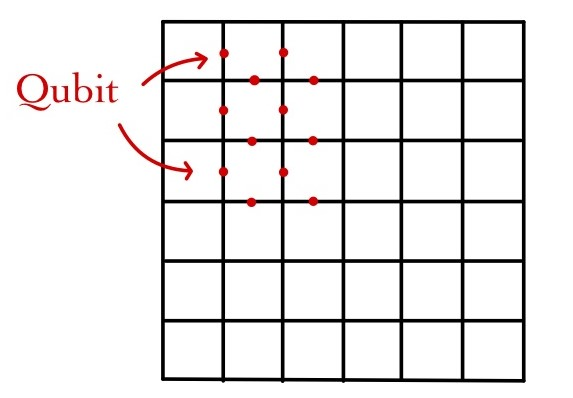
\includegraphics[scale=.43,keepaspectratio]{images/Toric_lattice_1}} \quad
	\subfloat[][Operatore $A_v$.\label{subfig:Toric_lattice_2} ]{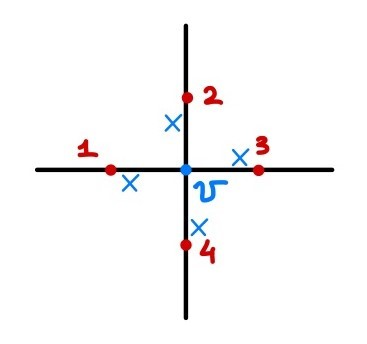
\includegraphics[scale=.43,keepaspectratio]{images/Toric_lattice_2}} \quad 
	\subfloat[][Operatore $B_p$.\label{subfig:Toric_lattice_3} ]{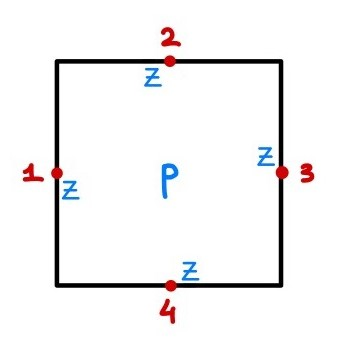
\includegraphics[scale=.43,keepaspectratio]{images/Toric_lattice_3}}
	\caption{\eqref{subfig:Toric_lattice_1} Reticolo $L \times L$ costituito da $2L^2$ qubit indipendenti. Per ogni plaquette ci sono 2 qubit indipendenti, quello in basso e quello a sinistra. \eqref{subfig:Toric_lattice_2} L'operatore rappresentato è esplicitamente $A_v = X_1 X_2 X_3 X_4$. \eqref{subfig:Toric_lattice_3} L'operatore rappresentato è esplicitamente $B_p = Z_1 Z_2 Z_3 Z_4$.}
    \label{fig:Toric_lattice}
\end{figure}

\noindent Il codice fu proposto per la prima volta dal fisico Alexei Kitaev ed è realizzato su un reticolo con condizioni al bordo periodiche (PBC: Periodic Boundary Conditions): dal punto di vista topologico considerare PBC sul quadrato di Figura \ref{subfig:Toric_lattice_1} significa porre il reticolo di qubit su un \textbf{toro} (il reticolo è bidimensionale, ma il volume è tridimensionale). Per realizzazioni concrete il toro risulta tuttavia poco pratico: in realtà la fisica del codice può essere ben rappresentata anche mediante strutture planari con opportune condizioni al bordo (per tale motivo il codice è anche detto \textbf{surface code}); anche l'idea di realizzazione di questa procedura su strutture planari fu proposta da Kitaev.

\noindent Ancora una volta la logica del codice è la stessa di quelle viste nelle precedenti sezioni perché è un \textbf{stabilizer code}. Vi sono due tipologie di stabilizers: per ogni vertice $v$ del reticolo si costruisce un operatore $A_v$ dato dal prodotto degli \texttt{X-gate} di ogni link appartenente al vertice e, similmente, per ogni faccia $p$ del reticolo (detta \textbf{plaquette}) si definisce l'operatore $B_p$ come prodotto dei 4 \texttt{Z-gate} sui link della plaquette. Si faccia riferimento alle Figure \ref{subfig:Toric_lattice_2} e \ref{subfig:Toric_lattice_3} per una rappresentazione grafica di questi operatori (chiaramente, così come i qubit, anche i gate si trovano sui link del reticolo). Dal punto di vista degli operatori avremo 
\begin{equation}\label{A_B}
    A_v = \prod_{j \in v} X_j \, , \qquad B_p = \prod_{j \in p} Z_j \, .
\end{equation}
In totale si hanno $L^2$ differenti operatori $A_v$ (uno per ognuno degli $L^2$ vertici) e $L^2$ differenti operatori $B_p$ (uno per ognuna delle $L^2$ plaquette): abbiamo quindi $2L^2$ differenti stabilizers. L'idea è, come al solito negli stabilizer codes, quello di codificare i qubit logici nel sottospazio (dato un certo autovalore) di questo insieme di operatori: più precisamente sappiamo che possiamo codificare il codewords nell'autospazio comune di questi operatori se commutano tra loro e il loro quadrato è l'identità. È evidente che per ogni $v$ e $p$, in quanto prodotto di matrici di Pauli, avremo $A^2_v = B^2_p = \mathbb{I}$. Inoltre si ha
\begin{equation}\label{commutatori_A_B}
    \comm{A_v}{B_p} = 0 \, , \qquad \comm{A_v}{A_{v'}} = 0 \, , \qquad \comm{B_p}{B_{p'}} = 0 \, \, \quad \forall \, v,p,v',p' \, ;
\end{equation}
il secondo e il terzo commutatore sono banali, tuttavia il primo è meno ovvio. Chiaramente questo commutatore è nullo quando $A_v$ e $B_p$ agiscono su qubit diversi (vertice e plaquette disgiunti), tuttavia potrebbe non essere nullo nel caso in cui $A_v$ sia localizzato in uno dei quattro vertici di una plaquette $p$ (si pensi al vertice \ref{subfig:Toric_lattice_2} posto su uno dei quattro vertici della plaquette \ref{subfig:Toric_lattice_3}): nonostante questa situazione, le matrici $X$ e $Z$ che agiscono sui qubit di un medesimo sottospazio sono sempre 2. Questo significa che i due anticommutatori $\acomm{Z_i}{X_i} = 0$ producono $(-1)^2 = 1$, quindi anche in questo caso il primo commutatore è dimostrato. 

\noindent Possiamo definire come codewords il sottospazio di $\mathcal{H}$ corrispondente all'autospazio comune agli operatori $A_v$ e $B_p$ con autovalore $+1$, ossia
\begin{equation*}
    C = \{ \text{Sottospazio comune agli operatori con autovalore } A_v = B_p = +1 \} \, .
\end{equation*}
Qual è la dimensione di $C$? Ricordando dalla \eqref{A_B} che gli stabilizers sono prodotti di matrici di Pauli, essi "tagliano" sempre $\mathcal{H}$ in due sottospazi della medesima dimensione: dato che abbiamo $L^2$ operatori $A_v$ e $L^2$ operatori $B_p$ allora si ha $\dim C = 2^{2L^2}/2^{L^2}/2^{L^2} = 1$, quindi sembrerebbe che non possiamo codificare i qubit in $C$. Il problema è che ci siamo dimenticati che non tutti questi stabilizers sono indipendenti! Essi soddisfano infatti
\begin{equation}\label{constraint_A_B}
    \prod_v A_v = \mathbb{I} \, , \qquad \prod_p B_p = \mathbb{I} \, ;
\end{equation}
queste proprietà derivano dal fatto che nei prodotti di tutti i possibili vertici e plaquette ci sono sempre almeno 2 matrici di Pauli in comune tali che $X_i^2 = \mathbb{I}$ e $Z_i^2 = \mathbb{I}$. Si pensi ad esempio all'operatore $A_{v_1}$ della Figura \ref{subfig:Toric_lattice_2} adiacente ad un altro $A_{v_2}$, i quali hanno un link in comune e quindi gli \texttt{X-gate} di quel link daranno $X^2 = \mathbb{I}$; discorso simile per due plaquette adiacenti $B_{p_1}$ e $B_{p_2}$ della Figura \ref{subfig:Toric_lattice_3}, le quali hanno un link comune che darà $Z^2 = \mathbb{I}$. I vincoli \eqref{constraint_A_B} fanno sì che si abbiano in totale  $(L^2-1) + (L^2-1)$ operatori $A_v$ e $B_p$ indipendenti: dunque il codewords ha dimensione 
\begin{equation*}
    \dim C = 2^{2 L^2} / 2^{L^2-1} / 2^{L^2-1} = 4 \, .
\end{equation*}
Questo significa che nel toro  possiamo codificare fino a 4 stati logici, ovvero 2 qubit logici. In realtà nel caso planare  si ha $\dim C = 2$, quindi possiamo codificare un singolo qubit logico (come nei codici precedenti). 

\noindent Come costruiamo gli stati logici del codewords $C$? Possiamo procedere in maniera esattamente analoga al caso di Steane: partiamo dallo stato $\ket{000 \ldots 0}$ (prodotto tensoriale dei $2L^2$ qubit indipendenti del reticolo) e calcoliamo 
\begin{equation}\label{logical_00}
    \ket{\overline{00}} = \prod_v \frac{(\mathbb{I}+A_v)}{\sqrt{2}} \ket{000 \ldots 0} \, ;
\end{equation}
sappiamo che in questo modo otteniamo automaticamente un autostato di qualsiasi $A_v$ con autovalore $+1$ perché $A_v (\mathbb{I} + A_v) \ket{\psi} = (A_v + \mathbb{I}) \ket{\psi}$. Analogamente avremo che $\ket{\overline{00}}$ è anche autostato di ogni $B_p$ con autovalore $+1$ perché valgono i commutatori \eqref{commutatori_A_B} e perché $B_p$ è un prodotto di \texttt{Z-gate} ($Z \ket{0} = \ket{0}$):
\begin{equation*}
    B_p (\mathbb{I} + A_v) \ket{000 \ldots 0} = (\mathbb{I} + A_v) B_p \ket{000 \ldots 0} = (\mathbb{I} + A_v) \ket{000 \ldots 0} \, .
\end{equation*}
In aggiunta allo stato $\ket{\overline{00}}$, dato che $\dim C = 4$, ci sono altri 3 stati logici che chiamiamo $\ket{\overline{01}}$, $\ket{\overline{10}}$ e $\ket{\overline{11}}$. Al posto che costruirli scrivendo formule analoghe alla \eqref{logical_00} possiamo identificare degli opportuni operatori logici $\overline{X}_1$, $\overline{X}_2$, $\overline{Z}_1$ e $\overline{Z}_2$ tali che permettano di costruire questi ultimi a partire da $\ket{\overline{00}}$: $\overline{X}_1 \ket{\overline{00}} = \ket{\overline{10}}$, ecc. Come riferimento grafico per la discussione che segue si vedano i due reticoli di Figura \ref{fig:logical_X_Z}.   

\begin{figure}[!h]
	\centering	
	\subfloat[][Operatori logici $\overline{Z}_1$ e $\overline{Z}_2$.\label{subfig:logical_X_Z_1} ]{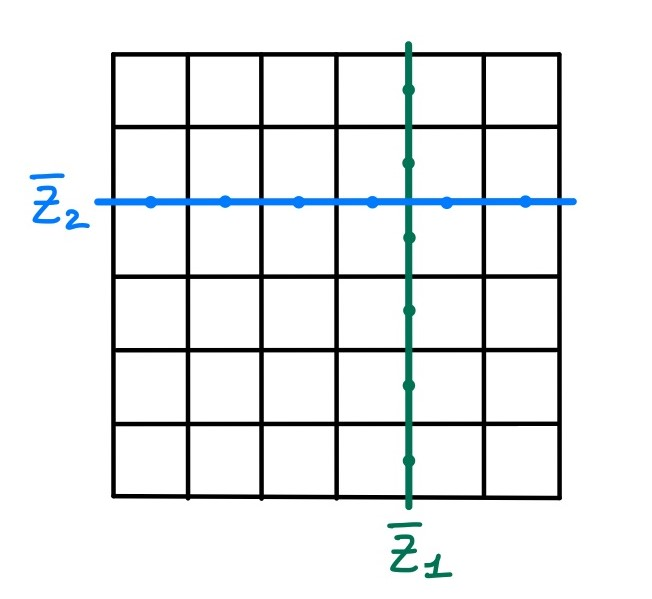
\includegraphics[scale=.43,keepaspectratio]{images/logical_X_Z_1}} \quad
	\subfloat[][Operatori logici $\overline{X}_1$ e $\overline{X}_2$.\label{subfig:logical_X_Z_2} ]{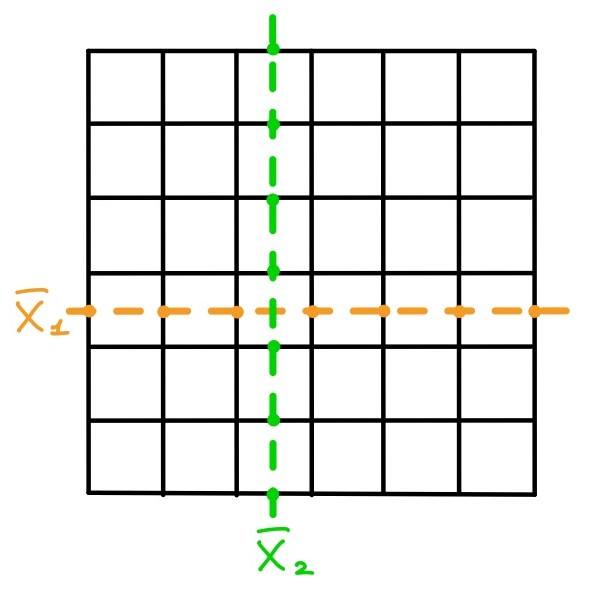
\includegraphics[scale=.43,keepaspectratio]{images/logical_X_Z_2}} 
	\caption{Le linee che rappresentano gli operatori logici $\overline{Z}_1$, $\overline{Z}_2$, $\overline{X}_1$ e $\overline{X}_2$ non sono altro che linee chiuse grazie alle PBC, quindi sono loop attorno al reticolo toroidale. I pallini rappresentati in corrispondenza dei link indicano i singoli gate che costituiscono il prodotto di quell'operatore logico.}
    \label{fig:logical_X_Z}
\end{figure}

\noindent Come mostrato nella Figura \ref{subfig:logical_X_Z_1}, definiamo $\overline{Z}_1$ come il prodotto di tutti gli \texttt{Z-gate} individuati dall'intersezione della linea verticale passante per i link del reticolo; similmente $\overline{Z}_2$ è definito come il prodotto degli \texttt{Z-gate} individuati dall'intersezione della linea orizzontale passante per i link. Esplicitamente avremo
\begin{equation}\label{logical_Z_1_2}
    \overline{Z}_1 = \prod_{i \in \text{vline}} Z_i \, , \qquad \overline{Z}_2 = \prod_{i \in \text{hline}} Z_i \, ,
\end{equation}
dove le diciture "vline" e "hline" indicano rispettivamente la linea verticale e la linea orizzontale passante per i link del reticolo. 

\noindent Similmente agli operatori \eqref{logical_Z_1_2} consideriamo ora la Figura \ref{subfig:logical_X_Z_2}. Se consideriamo questa volta il \textbf{reticolo duale}, ossia l'analogo reticolo che si costruisce passando per i punti medi dei link del reticolo di partenza, possiamo definire $\overline{X}_2$ come prodotto degli \texttt{X-gate} intercettati dalla linea verticale passante per il reticolo duale; infine definiamo $\overline{X}_1$ come prodotto degli \texttt{X-gate} intercettati dalla linea orizzontale passante per il reticolo duale. In termini di operatori scriviamo
\begin{equation}\label{logical_X_1_2}
    \overline{X}_1 = \prod_{i \in \text{hline}} X_i \, , \qquad \overline{X}_2 = \prod_{i \in \text{vline}} X_i \, ,
\end{equation}
dove questa volta le diciture "hline" e "vline" indicano rispettivamente la linea orizzontale e la linea verticale passante per i link del reticolo duale. È importante notare che grazie alle PBC le linee degli operatori $\overline{Z}_1$, $\overline{Z}_2$, $\overline{X}_1$ e $\overline{X}_2$ rappresentate nella Figura \ref{fig:logical_X_Z} non sono altro che \textbf{loop} (linee chiuse) passanti attorno al reticolo toroidale. D'ora in avanti ci riferiremo a queste linee chiamandole equivalentemente con il termine "loop".  

\noindent Come possiamo essere certi che gli operatori \eqref{logical_Z_1_2} e \eqref{logical_X_1_2} siano i corretti operatori logici? Sappiamo che gli operatori logici agiscono sul sottospazio $C$ e producono un nuovo stato $\ket{\psi} \in C$; questo significa che se gli operatori appena definiti commutano con tutti gli $A_v$ e $B_p$ allora la loro azione su stati del codewords produce altri stati di $C$, altrimenti, se anticommutano con $A_v$ e $B_p$, la loro azione su $C$ produce nuovi stati non più facenti parte del codewords, ossia si tratta di operatori corrispondenti ad errori. In altre parole dobbiamo quindi verificare che per ogni $i = 1 ,2$ e per qualsiasi $v$ e $p$ avremo
\begin{align}
    \comm{ \,\overline{X}_i}{ A_v} &= 0 \, , &\comm{ \,\overline{Z}_i}{ B_p} &= 0 \label{comm_log_banali} \\
    \comm{ \,\overline{X}_i}{ B_p} &= 0 \, , &\comm{ \,\overline{Z}_i}{ A_v} &= 0 \, . \label{comm_log_meno_banali}
\end{align}
Chiaramente, ricordando le definizioni \eqref{A_B}, le \eqref{comm_log_banali} sono banali. Per quanto riguarda invece le \eqref{comm_log_meno_banali} il discorso è più sottile: se si considerano operatori $A_v$ (vertici di Figura \ref{subfig:Toric_lattice_2}) e $B_p$ (plaquette di Figura \ref{subfig:Toric_lattice_3}) disgiunti rispetto alle linee individuate rispettivamente da $\overline{Z}_i$ e $\overline{X}_i$ allora i commutatori sono ancora una volta banali. Se si considera tuttavia un vertice $A_v$ sulla linea $\overline{Z}_i$ allora esso presenterà alcuni operatori agenti sul medesimo sottospazio di quelli del loop: gli \texttt{X-gate} di $A_v$ sul loop $\overline{Z}_i$ saranno sempre due (sopra e sotto per $\overline{Z}_1$ e destra e sinistra per $\overline{Z}_2$), quindi come per \eqref{commutatori_A_B}, le due anticommutazioni producono $(-1)^2 = +1$ e il commutatore è dimostrato. Vale un discorso analogo per gli operatori $B_p$: quando la plaquette di $B_p$ si interseca con una delle due linee $\overline{X}_i$ allora saranno sempre e solamente 2 gli \texttt{Z-gate} di $B_p$ agenti sul medesimo sottospazio degli \texttt{X-gate} del loop $\overline{X}_i$ (sopra e sotto per $\overline{X}_2$ e destra e sinistra per $\overline{X}_1$); perciò le due anticommutazioni producono come prima $(-1)^2 = +1$ e il commutatore è verificato\footnote{Per capire ancora meglio questo discorso si provi a sovrapporre gli operatori $A_v$ e $B_p$ delle Figure \ref{subfig:Toric_lattice_2} e \ref{subfig:Toric_lattice_3} con le linee delle Figure \ref{subfig:logical_X_Z_1} e \ref{subfig:logical_X_Z_2} rispettivamente: apparirà evidente come sono sempre due gli operatori anticommutanti agenti sul medesimo sottospazio.}.

\noindent Affinché $\overline{Z}_1$, $\overline{Z}_2$, $\overline{X}_1$ e $\overline{X}_2$ siano i corretti operatori logici non solo devono essere verificati i commutatori sopra, ma inoltre deve valere
\begin{equation*}
    \acomm{\overline{X}_1}{\overline{Z}_1} = 0 \, , \qquad \acomm{\overline{X}_2}{\overline{Z}_2} = 0 \, ;
\end{equation*}
queste relazioni sono ovvie se si pensano ai loop di Figura \ref{fig:logical_X_Z}: nell'intersezione di $\overline{X}_1$ con $\overline{Z}_1$ e di $\overline{X}_2$ con $\overline{Z}_2$ vi è precisamente un solo operatore ($X$ per $\overline{X}_i$ e $Z$ per $\overline{Z}_i$) che agisce sul medesimo sottospazio comune perché l'intersezione tra le due linee avviene in un solo punto. Questo fatto fa in modo che grazie all'anticommutatore $\acomm{X}{Z} = 0$ gli anticommutatori logici precedenti siano anch'essi verificati.  

\noindent Dati quindi gli operatori logici in \eqref{logical_Z_1_2} e \eqref{logical_X_1_2} possiamo calcolare i 3 stati logici rimanenti ($\ket{\overline{01}}$, $\ket{\overline{10}}$ e $\ket{\overline{11}}$) a partire dallo stato \eqref{logical_00}. Nonostante ciò qui si evidenzia la natura topologica del codice: avremmo potuto proporre come operatori logici moltissimi altri loop oltre alle linee di Figura \ref{fig:logical_X_Z}, ma ciò non avrebbe fatto alcuna differenza perché si tratta sempre di loop omotopi a quelle linee!

\noindent Il motivo profondo dell'affermazione precedente è mostrato nell'esempio di Figura \ref{fig:topological_loops}. 

\begin{figure}[!ht]
    \centering
    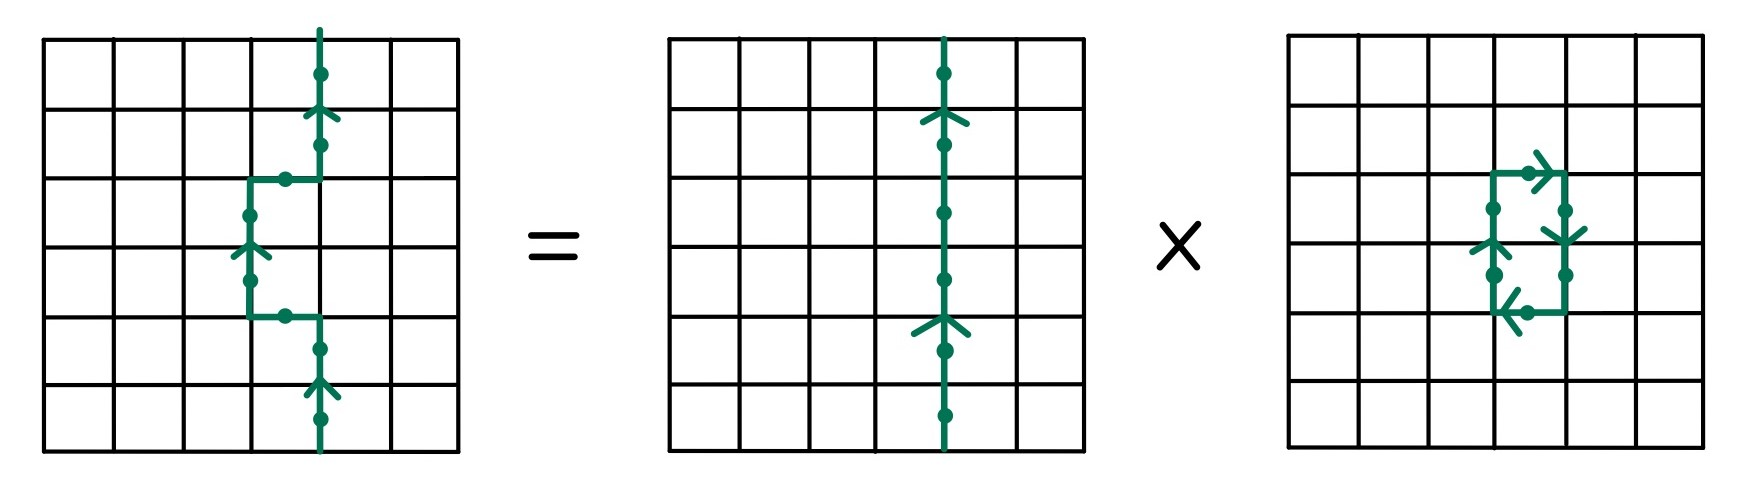
\includegraphics[scale=0.33]{images/topological_loops}
    \caption{Una possibile scelta di operatore logico $\overline{Z}_1$ è dato dal loop spezzato a sinistra. Questo loop è in realtà equivalente al loop dritto della Figura \ref{subfig:logical_X_Z_1} per il loop chiuso a destra, il quale è omotopo a zero, ossia all'identità quando agisce sul codewords.}
    \label{fig:topological_loops}
\end{figure}

\noindent Nella parte sinistra della figura è presentato un esempio di scelta differente di $\overline{Z}_1$, il quale non è altro che un loop (linea) lungo il toro che non è più dritto. Si può infatti dimostrare con argomenti analoghi ai precedenti che è un operatore logico $\overline{Z}_1$ perché soddisfa i commutatori \eqref{comm_log_banali} e \eqref{comm_log_meno_banali}.  Sembrerebbe da questa scelta che possiamo avere un'infinità di loop analoghi, tuttavia ora dimostriamo che in realtà il loop a sinistra è equivalente al prodotto del loop dritto al centro della Figura \ref{fig:topological_loops} (ossia quello della Figura \ref{subfig:logical_X_Z_1}) per il loop chiuso a destra, dove quest'ultimo è dato dal prodotto di tutti gli \texttt{Z-gate} lungo tale loop. Per capire questo fatto consideriamo il loop chiuso a destra: con la stessa logica possiamo pensare a questo loop, che circonda due plaquette, come al prodotto dei due loop più piccoli che circondano ciascuno una singola plaquette. In tale situazione il link orizzontale intermedio comune ai due loop conta 2 operatori $Z$, ciascuno da uno dei due loop: grazie alla proprietà $Z^2 = \mathbb{I}$ allora effettivamente questo loop attorno alle due plaquette è equivalente al prodotto dei due loop singoli. 

\noindent Quale sarà il loop più piccolo possibile? Chiaramente questo non è altro che il prodotto di 4 \texttt{Z-gate} attorno ad una plaquette, ossia, dalla definizione \eqref{A_B}, proprio lo stabilizer $B_p$ di Figura \ref{subfig:Toric_lattice_3}; ma ricordiamo che ciascun $B_p$ sul codewords ha autovalore $+1$! Questo significa che ciascun loop non dritto del reticolo è equivalente ad un loop dritto (Figura \ref{subfig:logical_X_Z_1}) grazie al fatto che ogni loop chiuso abbia un contributo banale su $C$: 2 loop omotopi sono equivalenti quando agiscono sul codewords! È questo il motivo fondamentale per cui il codice è chiamato \textbf{topologico}: è possibile deformare i contorni di $\overline{Z}_i$ e $\overline{X}_i$ senza cambiare l'azione di questi operatori logici sugli stati del codewords!

\noindent Notiamo che con la stessa logica precedente un qualsiasi prodotto di \texttt{Z-gate} lungo un loop chiuso contraibile è equivalente all'identità quando agisce su $C$:
\begin{equation}\label{product_Z_closed_loop}
    \prod_{i \in \substack{\text{loop} \\ \text{chiuso}\\ \text{contraibile}}} Z_i \equiv \mathbb{I} \, \text{ agendo su } C \, .
\end{equation}
Perciò il contributo del prodotto precedente è banale su $C$ perché un qualsiasi loop chiuso può essere decomposto come prodotto di plaquette singole, ossia come prodotto di $B_p$, le quali hanno autovalore $+1$ sul codewords. Questo fatto può essere espresso in altre parole dicendo che qualsiasi loop chiuso contraibile sia omotopo a zero, ossia è equivalente all'azione dell'identità sul codewords. 

\noindent Qual è quindi la ragione per cui abbiamo esattamente 4 operatori logici non banali? Il motivo è che qualsiasi operatore non banale sul toro deve essere periodico: i due loop della Figura \ref{fig:torus} (ricordare che sono prodotti di operatori), a differenza di qualsiasi altro loop, non sono omotopi a zero e ciascuno dei due può essere costituito dal prodotto di \texttt{Z-gate} oppure \texttt{X-gate}. Abbiamo quindi in totale 4 operatori non banali (2 loop non-contraibili con prodotti di $Z$ più 2 loop con prodotti di $X$). 

\begin{figure}[!h]
    \centering
    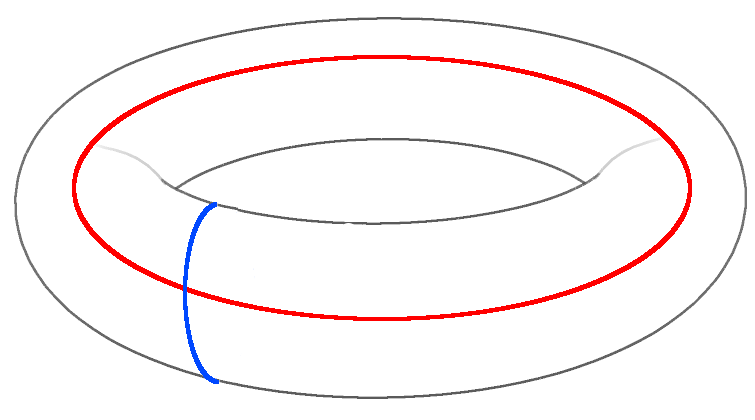
\includegraphics[scale=0.33]{images/torus}
    \caption{Abbiamo in totale 4 operatori logici non banali: 2 loop rossi e 2 loop blu . Ogni tipologia di loop (rosso o blu) può essere originata da prodotti di \texttt{Z-gate} o \texttt{X-gate}. Qualsiasi altro loop non rappresentato in figura è banale, ossia è omotopo a zero e agisce come un'identità sul codewords. Notare che questi 4 operatori, se pensati in una rappresentazione planare con PBC, non sono altro che le 4 linee (loop) delle Figure \ref{subfig:logical_X_Z_1} e \ref{subfig:logical_X_Z_2}.}
    \label{fig:torus}
\end{figure}

\subsection{Correzione degli errori}
Discutiamo ora come avviene la correzione degli errori nel toric code. Ricordiamo ancora una volta che negli stabilizer codes gli operatori commutanti con gli stabilizers sono operatori logici, mentre coloro che non commutano, ma anticommutano, sono errori.

\begin{figure}[!ht]
	\centering	
	\subfloat[][Bit flip error.\label{subfig:bit_phase_toric_1} ]{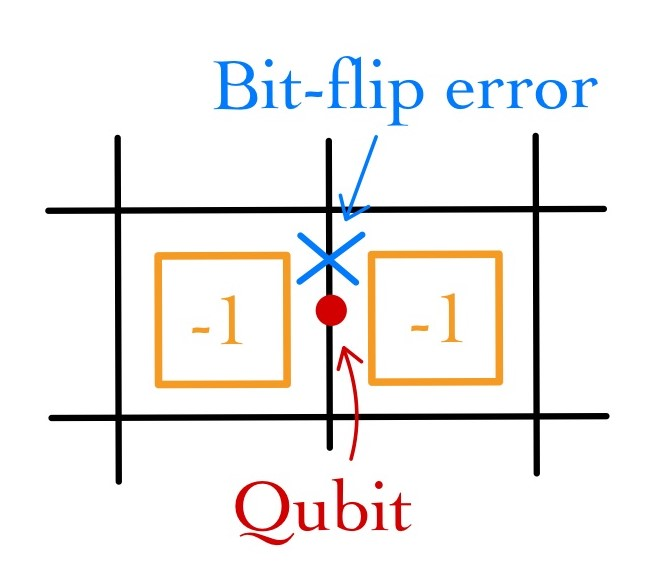
\includegraphics[scale=.32,keepaspectratio]{images/bit_phase_toric_1}} \quad
	\subfloat[][Phase flip error.\label{subfig:bit_phase_toric_2} ]{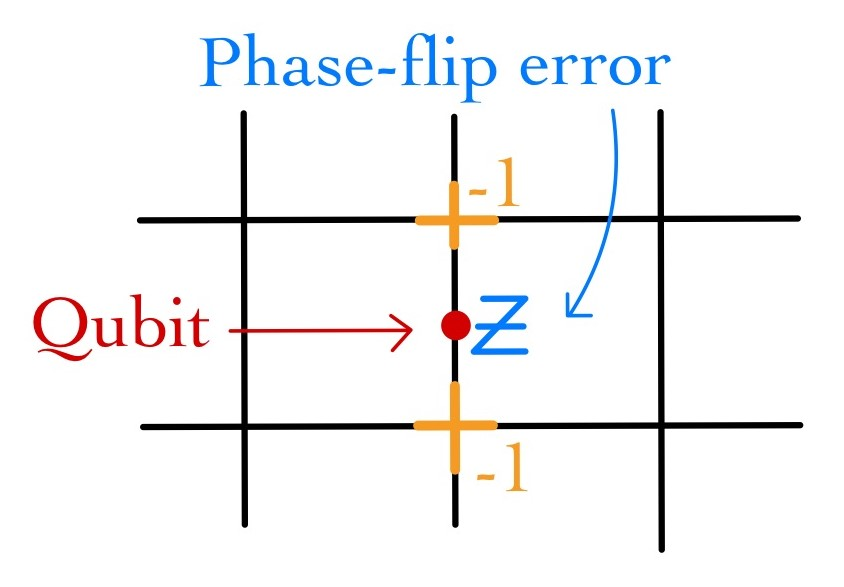
\includegraphics[scale=.32,keepaspectratio]{images/bit_phase_toric_2}} 
	\caption{(\ref{subfig:bit_phase_toric_1}) Esempio di rilevazione di un bit flip error. Solamente le due plaquette (riquadri arancioni) adiacenti all'errore contano perché viene invertito il loro autovalore. (\ref{subfig:bit_phase_toric_2}) Esempio di rilevazione di un phase flip error. Solamente i due vertici (croci arancioni) adiacenti all'errore contano perché viene invertito il loro autovalore.}
    \label{fig:bit_phase_toric}
\end{figure}

\noindent Cominciamo col considerare un \textbf{bit flip error}. Immaginiamo, come in Figura \ref{subfig:bit_phase_toric_1}, di avere un qubit su un link qualsiasi con un errore dato da un \texttt{X-gate}.  In tale situazione solamente le due plaquette adiacenti al link contano: in generale $\comm{X}{A_v} = 0$, ma dato che $B_p = \prod_{j \in p} Z_j$ allora solamente per le due plaquette mostrate avremo $\comm{X}{B_p} \neq 0$. Dato che in particolare si ha $\acomm{X}{B_p} = 0$ per la presenza di uno \texttt{Z-gate} agente sullo stesso sottospazio di $X$ in ciascuna delle due plaquette, allora l'autovalore di questi due $B_p$ su $C$ è diventato $-1$. In questo modo possiamo rilevare un bit flip error misurando l'autovalore di queste due plaquette. Questo significa, in generale, che quando si ha una situazione in cui tutti gli operatori $B_p$ hanno autovalore $+1$ eccetto per due plaquette adiacenti allora sia ha la certezza che è presente un bit flip error nel qubit tra le due. 

\noindent Consideriamo ora un \textbf{phase flip error}. Come evidenziato nella Figura \ref{subfig:bit_phase_toric_2} la situazione è simile alla precedente, ma questa volta l'errore è rappresentato da uno \texttt{Z-gate} su un link: per ogni plaquette avremo $\comm{Z}{B_p} = 0$, ma essendo $A_v = \prod_{i \in v} X_i$ allora per i due vertici adiacenti mostrati si ha $\comm{Z}{A_v} \neq 0$. Come in precedenza, l'errore agisce sul medesimo sottospazio degli operatori $X$ nei due $A_v$, quindi a causa dell'anticommutatore $\acomm{Z}{A_v} = 0$ l'autovalore di questi due vertici sarà $-1$. Esattamente come il caso precedente, quando tutti gli operatori $A_v$ hanno autovalore $+1$ tranne due vertici adiacenti allora si ha la certezza che è presente un phase flip error nel qubit tra i due. 

\noindent Ricapitolando, abbiamo esplicitamente mostrato che gli operatori $A_v$ e $B_p$ agiscono come stabilizers: misurando gli autovalori degli \eqref{A_B} è possibile rilevare direttamente bit flip error e phase flip error. Gli altri errori, ossia la combinazione bit-phase flip, sono semplicemente dati da una combinazione dei casi precedenti. 

\noindent Una delle ragioni principali per cui questo codice di correzione degli errori è così popolare nella letteratura del QC è data dal fatto che sia possibile rilevare e correggere gli errori aggiungendo qubit extra (che chiamiamo anche qui \textbf{ancilla qubits}) nei vertici e nelle facce del reticolo. Tutte le tipologie di qubit presenti nel reticolo (compresi gli ancilla) sono mostrate in Figura \ref{subfig:ancilla_toric_1}. I qubit sui link (pallini rossi pieni) sono i qubit fisici, ossia coloro che codificano l'informazione. Viceversa, i qubit aggiunti sui vertici e al centro delle facce del reticolo (pallini arancio vuoti) sono gli ancilla qubit che hanno lo scopo di effettuare la misurazione e correggere eventuali errori. Chiamiamo \textbf{qubit of type Z} gli ancilla nelle facce perché effettuano la misurazione di $B_p$ sui 4 qubit dei link della plaquette, mentre definiamo \textbf{qubit of type X} gli ancilla presenti nei vertici, i quali similmente effettuano una misurazione di $A_v$ sui 4 qubit dei link entranti in quel vertice.

\noindent Più precisamente, consideriamo la singola plaquette di qubit di Figura \ref{subfig:ancilla_toric_2}. L'ancilla qubit effettua una misurazione dell'operatore $B_p = Z_1 Z_2 Z_3 Z_4$: questa misurazione può essere portata a termine per mezzo del seguente circuito
\begin{center}
    \mbox{
        \Qcircuit @C=2em @R=1em {
            \lstick{\text{Ancilla: }\ket{0}} & \targ & \targ & \targ & \targ & \meter & \rstick{\ket{0}, \ket{1}} \qw \\
            \lstick{1} & \ctrl{-1} & \qw & \qw & \qw & \qw & \qw \\
            \lstick{2} & \qw & \ctrl{-2} & \qw & \qw & \qw & \qw \\
            \lstick{3} & \qw & \qw & \ctrl{-3} & \qw & \qw & \qw \\
            \lstick{4} & \qw & \qw & \qw & \ctrl{-4} & \qw & \qw
        }
    }
\end{center}
L'autovalore del prodotto dei 4 \texttt{Z-gate} di $B_p$ sarà $+1$ o $-1$ a seconda del numero di flip che vengono operati dai \texttt{CNOT-gate}: un numero dispari di stati $\ket{1}$ nei 4 qubit produrrà $B_p = -1$ perché l'ancilla sarà in $\ket{1}$, viceversa un numero pari di $\ket{1}$ vorrà dire $B_p = +1$ perché la misurazione sull'ancilla ha output $\ket{0}$. Misurando quindi lo stato dell'ancilla siamo in grado di stabilire l'autovalore di $B_p$. 

\begin{figure}[!ht]
	\centering	
	\subfloat[][Reticolo di qubit.\label{subfig:ancilla_toric_1} ]{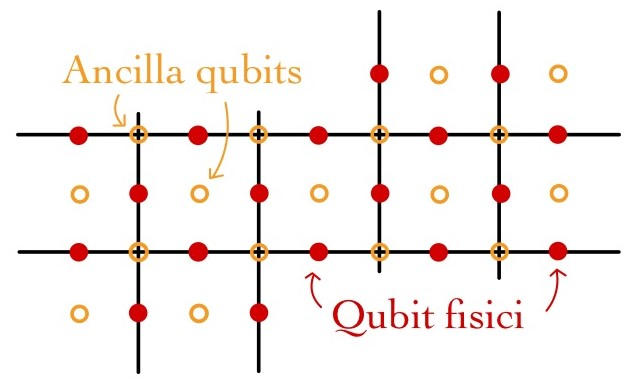
\includegraphics[scale=.45,keepaspectratio]{images/ancilla_toric_1}} \quad
	\subfloat[][Misura di $B_p$.\label{subfig:ancilla_toric_2} ]{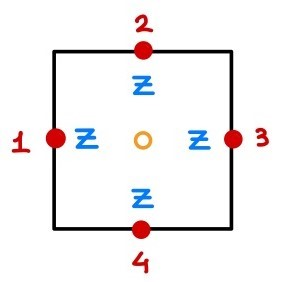
\includegraphics[scale=.45,keepaspectratio]{images/ancilla_toric_2}} \quad
	\subfloat[][Misura di $A_v$.\label{subfig:ancilla_toric_3} ]{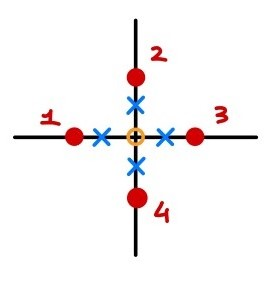
\includegraphics[scale=.45,keepaspectratio]{images/ancilla_toric_3}}
	\caption{Il reticolo è cosparso di qubit fisici (pallini rossi pieni sui link) e di ancilla qubits (pallini arancio vuoti nelle facce e sui vertici). Gli ancilla delle plaquette permettono di effettuare una misurazione dell'autovalore di $B_p$, mentre gli ancilla dei vertici effettuano una misura dell'autovalore di $A_v$.}
    \label{fig:ancilla_toric}
\end{figure}

\noindent In maniera del tutto analoga consideriamo ora il singolo vertice di Figura \ref{subfig:ancilla_toric_3}. È possibile dimostrare che l'ancilla sul vertice effettua una misurazione dell'operatore $A_v = X_1 X_2 X_3 X_4 $ utilizzando un circuito analogo al precedente (vengono solamente inseriti alcuni \texttt{H-gate}): anche in questo caso, una misurazione sullo stato finale dell'ancilla permette di stabilire se l'autovalore è $A_v = +1$ oppure $A_v = -1$. 

\noindent Analizziamo ora gli errori mostrati in Figura \ref{subfig:strange_errors_toric_1}. Come evidenziato anche nella Figura \ref{subfig:bit_phase_toric_1}, la misura nel reticolo di due autovalori $B_p = -1$ corrisponde ad un bit flip error sul qubit tra le due plaquette adiacenti (situazione azzurra in alto nel reticolo). Nonostante la situazione precedente possono avvenire altre tipologie di errori: supponiamo di misurare due autovalori $B_p = -1$ in corrispondenza di due plaquette non adiacenti (si vedano i $-1$ in rosso nelle due facce). Da che cosa sono prodotti errori come i precedenti? Questi non sono altro che il risultato di una serie di bit flip lungo una linea che connette le due plaquette (si veda le "X" in arancio): dato che tutti i link tra le plaquette intermedie hanno cambiato segno due volte a seguito del bit flip, allora per tali facce la misura produce $B_p = +1$, mentre per le plaquette iniziali e finali l'autovalore risulta invertito! Siamo quindi in grado di dare una corretta interpretazione anche di questa tipologia di errore. 

\noindent Perché la natura topologica del codice è così importante? Come possiamo essere certi che l'errore appena spiegato sia dovuto alla linea arancio di bit flip e non, ad esempio, alla linea verde? In principio ogni possibile cammino di \texttt{X-gate} che connette le due plaquette invertite potrebbe dare lo stesso identico errore. Se non sappiamo distinguere quale percorso di \texttt{X-gate} ha causato l'errore, come possiamo correggerlo? Il punto fondamentale è che non importa quale sia il giusto percorso di errori: possiamo correggere gli errori applicando un cammino arbitrario di \texttt{X-gate} lungo un qualsiasi cammino aperto che connette le due plaquette invertite: si tratta quindi di scegliere un cammino di \texttt{X-gate} che connette le due plaquette invertite! Il cammino originale che causa l'errore (non lo conosciamo) più il cammino di \texttt{X-gate} scelto è un operatore banale perché uno compensa l'altro: il percorso finale risultante non è altro che un cammino chiuso nel reticolo duale, quindi la combinazione di errori risulta in un prodotto di \texttt{X-gate} lungo un loop chiuso (Figura \ref{subfig:strange_errors_toric_2})! Dato che, come illustra la Figura \ref{subfig:strange_errors_toric_2}, un qualsiasi prodotto di \texttt{X-gate} su un loop chiuso contraibile può essere scritto come prodotto di $A_p$, allora in analogia alla \eqref{product_Z_closed_loop} avremo
\begin{equation}\label{product_X_closed_loop}
    \prod_{i \in \substack{\text{loop} \\ \text{chiuso}\\ \text{contraibile}}} X_i \equiv \mathbb{I} \, \text{ agendo su } C \, .
\end{equation}

\begin{figure}[!ht]
	\centering	
	\subfloat[][\label{subfig:strange_errors_toric_1} ]{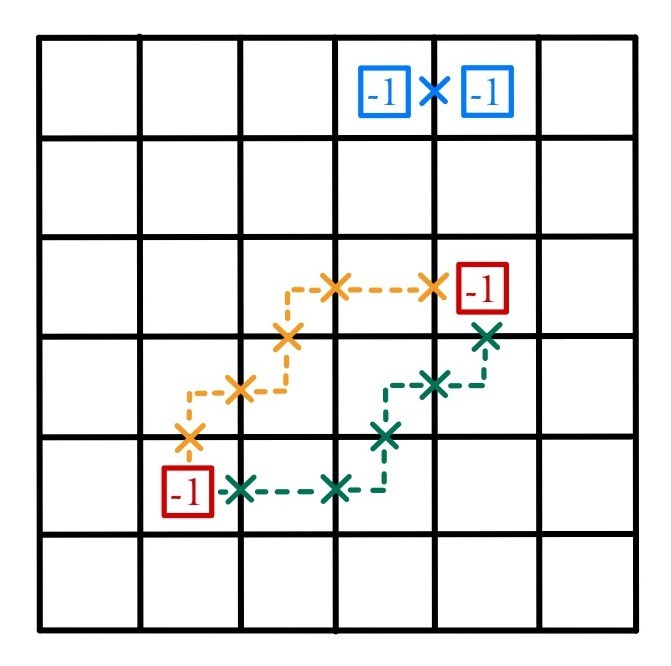
\includegraphics[scale=.38,keepaspectratio]{images/strange_errors_toric_1}} \qquad
	\subfloat[][\label{subfig:strange_errors_toric_2} ]{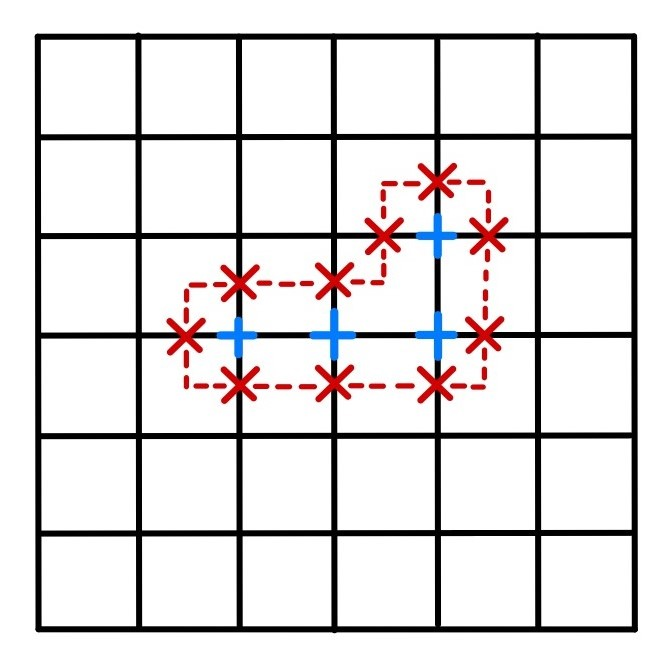
\includegraphics[scale=.38,keepaspectratio]{images/strange_errors_toric_2}}
	\caption{(\ref{subfig:strange_errors_toric_1}) La misura di due autovalori $B_p = -1$ in corrispondenza di due plaquette non adiacenti (facce in rosso) può essere causata da una concatenazione di bit flip errors lungo un cammino che connette le due plaquette. Per correggere tale errore basta applicare un percorso di \texttt{X-gate} che connette le due plaquette. (\ref{subfig:strange_errors_toric_2}) Un prodotto di \texttt{X-gate} su un loop chiuso nel reticolo duale è equivalente ad un prodotto di operatori $A_v$ (vertici azzurri), i quali hanno contributo banale su $C$.}
    \label{fig:strange_errors_toric}
\end{figure}

\noindent Ricapitolando: un cammino chiuso di \texttt{X-gate} nel reticolo duale può sempre essere visto come prodotto di tutti i vertici (operatori $A_v$) contenuti nel loop; ogni $A_p$ inserisce un \texttt{X-gate} sui link esterni mentre, grazie a $X^2 = \mathbb{I}$, nulla accade nei link interni comuni ai vertici. Dato che su $C$ tutti gli $A_p$ hanno autovalore $+1$, allora i loop chiusi di \texttt{X-gate} nel reticolo duale sono omotopi a zero, ossia sono l'operatore banale (identità). 

\subsection{Interpretazione in meccanica statistica}
Esiste una curiosa interpretazione del toric code alla luce della meccanica statistica considerando un reale modello di spin quantistici. Supponiamo un reticolo in cui, su ogni link, è possibile avere uno spin quantistico (up o down). In un tale sistema l'hamiltoniana è data da 
\begin{equation}\label{hamilt_toric}
    H = - J \sum_v A_v - J \sum_p B_p \, , \qquad J > 0 \, .
\end{equation}
Come mostra la Figura \ref{subfig:stat_mec_toric_1}, l'interazione degli spin avviene in due modi: interagiscono i 4 spin in un vertice (prima somma in $H$) oppure i 4 spin di una plaquette (seconda somma in $H$). Qual è lo stato (o gli stati) di minima energia? I ground state corrispondono a tutte quelle situazioni in cui gli autovalori sono $A_v = B_p = +1$ per ogni vertice e plaquette del reticolo. In un'interpretazione di questo tipo i 4 stati logici $\ket{\overline{00}}$, $\ket{\overline{01}}$, $\ket{\overline{10}}$ e $\ket{\overline{11}}$ (con autovalori $A_v = B_p = +1$) del QC sono mappati nei ground state dell'hamiltoniana \eqref{hamilt_toric}; viceversa gli errori nel reticolo corrispondono a delle eccitazioni, ossia a delle configurazioni in cui almeno un autovalore di $A_v$ e/o $B_p$ è uguale a $-1$. 

\begin{figure}[!ht]
	\centering	
	\subfloat[][\label{subfig:stat_mec_toric_1} ]{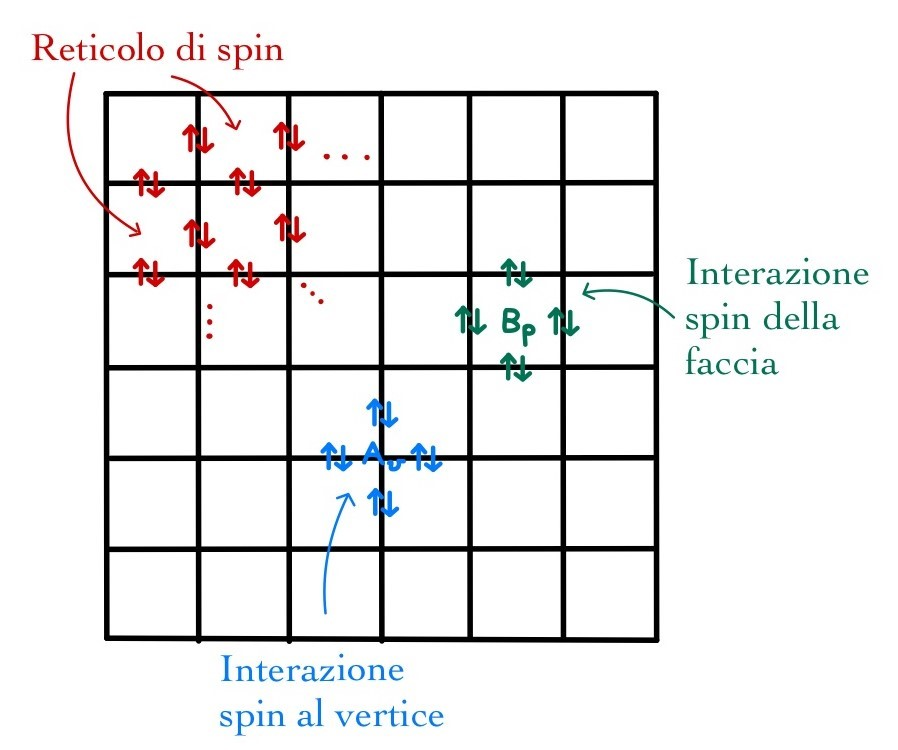
\includegraphics[scale=.35,keepaspectratio]{images/stat_mec_toric_1}} \quad
	\subfloat[][\label{subfig:stat_mec_toric_2} ]{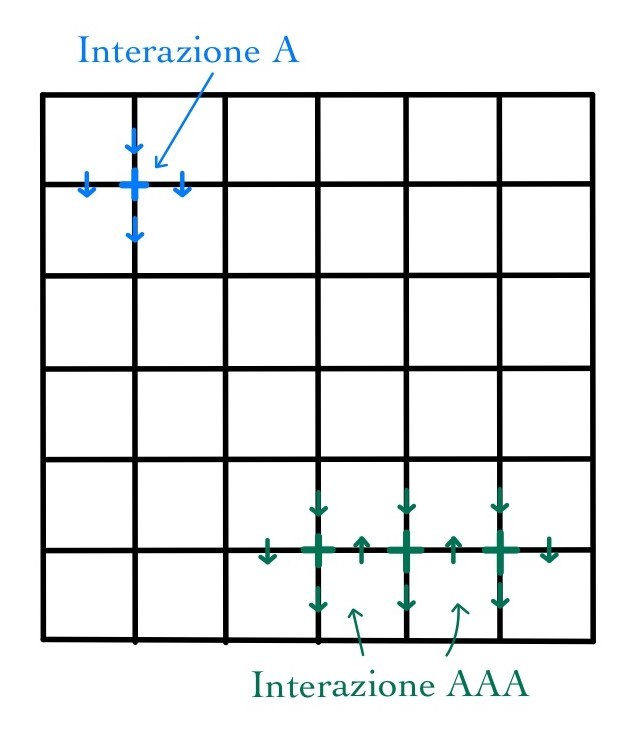
\includegraphics[scale=.35,keepaspectratio]{images/stat_mec_toric_2}}
	\caption{(\ref{subfig:stat_mec_toric_1}) L'analogo sistema in meccanica statistica del toric code è costituito da un reticolo di spin in cui questi ultimi possono interagire in un vertice oppure in una plaquette. (\ref{subfig:stat_mec_toric_2}) Se si espande la produttoria in \eqref{logical_00} si hanno diverse interazioni di spin a causa delle combinazioni degli operatori $A_v$.}
    \label{fig:stat_mec_toric}
\end{figure}

\noindent Dal punto di vista dei singoli spin lo stato \eqref{logical_00} è estremamente complicato perché è uno stato molto entangled. Se si espande la produttoria in $\ket{\overline{00}}$ si ottengono dei termini del tipo $\mathbb{I} + A + AA + AAA + \ldots$, quindi avvengono diverse interazioni: come illustra la Figura \ref{subfig:stat_mec_toric_2}, il singolo operatore $A$ agisce sul vertice e inverte i 4 spin (in blu in alto a sinistra dove gli spin $\uparrow$ sono diventati $\downarrow$); gli operatori della forma $AAA$, invece, creano un loop di spin capovolti nel reticolo originale (si vedano i tre vertici in basso in verde). In totale la produttoria in \eqref{logical_00} produce una sovrapposizione lineare di tutti i possibili loop costituiti da spin invertiti: c'è entanglement tra tutti gli spin del reticolo, persino tra quelli più distanti. 

\noindent Che cosa sono gli errori in QC? Non sono altro che operatori che agiscono sui link del reticolo: ad esempio se si pensa ad un singolo bit flip error (\texttt{X-gate} su un link) allora esso cambia autovalore agli operatori $B_p$ delle placchette adiacenti (si veda la Figura \ref{subfig:bit_phase_toric_1}); similmente quando si ha un phase flip error (Figura \ref{subfig:bit_phase_toric_2}), allora lo \texttt{Z-gate} sul link corrotto cambierà autovalore ai due operatori $A_v$ adiacenti. 

\noindent Data l'hamiltoniana \eqref{hamilt_toric}, agli errori nel QC corrispondono delle eccitazioni nel sistema di spin: avremo una variazione di energia $\Delta E_z = 2 J$ per il singolo phase flip e una variazione di $\Delta E_x = 2 J$ per il singolo bit flip. In teoria della materia condensata questi stati eccitati corrispondono alle cosiddette \textbf{quasiparticles}. In questo contesto ne esistono di due tipologie: le quasiparticle \textbf{elettriche}, a seguito dell'errore causato da $Z$ e le quasiparticle \textbf{magnetiche}, generate dall'errore di $X$; entrambe hanno la medesima energia e  vedremo nelle prossime sezioni che presentano alcune proprietà strane e insolite. Dato che per ogni errore (bit flip o phase flip) si hanno due autovalori $-1$ ($A_v = -1$ per $Z$ e $B_p = -1$ per $X$) allora è come se potessimo associare due paia di quasiparticle: 2 elettriche e 2 magnetiche. 

\noindent Una delle proprietà più insolite (vedremo) è la seguente: se si considera una quasiparticle elettrica e la si muove attorno ad una quasiparticle magnetica ritornando poi al punto di origine allora, a seguito della QM, si origina una fase: questo fenomeno può essere interpretato come un doppio scambio di particelle; per tale ragione questa particolare tipologia di particelle costituiscono un perfetto "toy model" per i cosiddetti \textbf{anyons} (diffusi in letteratura nella teoria della materia condensata). Queste particolari quasiparticle, presenti unicamente in sistemi bidimensionali, sono simili a particelle che presentano una statistica frazionaria, ossia non sono né bosoni né fermioni!
    \vspace{0.5cm}
\newline 
\noindent \lecture{15}{30/11/2021}
\vspace{0.5cm}
\noindent Nel caso in cui all'estremo dell'elettrodo ci siano due giunzioni, si parla di TRANSMON simmetrico.
\begin{figure}
    \centering
    \begin{circuitikz}
        \draw (0,0)
        to[barrier=$\Phi_e$] (0,2) 
        to[short] (2,2)
        to[C] (2,0) 
        to[short] (-2,0)
        to[barrier] (-2, 2)
        to[short] (0,2);
    \end{circuitikz}    
    
    \caption{}
\end{figure}
Questa configurazione permette di variare la corrente critica a piacimento, tramite l'applicazione del campo esterno $\Phi_e$:
\begin{equation*}
    I_0' = 2I_o \abs{\cos \frac{\pi \phi_e}{\phi_o}}
\end{equation*}
L'hamiltoniana, a questo punto, diventa:
\begin{equation*}
    H=4E_cn^2-2E_J\left|\cos(\pi\frac{\Phi_e}{\Phi_0})\right|\cos\delta
\end{equation*}
Perciò possiamo ora variare sia $E_C$ (progettando il circuito adeguatamente) e $E_J$ (tramite il campo esterno). L'anarmonicità risulta inoltre data da $\pi\frac{\Phi_e}{\Phi_0}=k\pi/2$ (con k interi). Abbiamo, dunque, la capacità di scegliere in modo arbitrario la frequenza di risonanza del qubit (caratteristica chiaramente necessaria, in particolare nel caso di utilizzo di più qubit contemporaneamente).
Si noti che differenti varianti del TRANSMON simmetrico sono state proposte (ad esempio usando due giunzioni differenti si può diminuire la dipendenza dal flusso esterno della frequenza del qubit).
Questo tipo di circuiti, tuttavia, porta con sé alcuni problemi di fabbricazione: in particolare le giunzioni devono avere dimensioni che non possono essere ottenute con litografia ottica (è necessaria la più complessa litografia a raggi ionici). Inoltre la produzione di tutti i componenti deve essere svolta nel medesimo vuoto in modo da avere superfici il più possibile uniformi.

\section{Controllo di un qubit}

\subsection{TRANSMON Qubit}

Il motivo per cui si utilizza la configurazione "a più" dell'XMON è che in questo modo abbiamo 3 punti di accoppiamento fra la giunzione e l'esterno. Tramite questi punti potremo leggere lo stato del qubit e modificarlo.
Il controllo del qubit (e dunque l'applicazione dei gate) viene detto \textit{XY control}: è costituito da una piccola capacità $C_d$ (\textit{d} di \textit{drive}, come viene chiamato il segnale) collegata a una sorgente \textit{RF} (la presenza della capacità serve a tenere separati i due componenti del circuito, in modo da non diminuire i tempi di decoerenza).
L'hamiltoniana del sistema, approssimando il qubit a un semplice oscillatore armonico, risulta (con $Q=\partialderivative{\mathcal L}{\dot{\Phi}}=\dot{\Phi}(C+C_d)$):
\begin{equation*}
    H_0 = \frac{Q^2}{2(C+C_d)^2} +\frac{\Phi^2}{2L}
\end{equation*}
Alla quale bisogna aggiungere un ulteriore termine di drive:
\begin{equation*}
    H_d = C_d \dot \Phi V_d(t)=\frac{C_d}{C+C_d}QV_d(t)
\end{equation*}
A questo punto possiamo scrivere (in funzione della carica di fluttuazione di punto zero $Q_{\text{ZPF}}=\sqrt{\frac{\hbar}{2z}}$, con $z=\sqrt{\frac{L}{C}}$):
\begin{equation*}
    Q= -i Q_{\text{ZPF}}(a - a^\dagger)
\end{equation*}
E infine possiamo scrivere l'hamiltoniana totale ($\omega_q=\frac{\sqrt{8E_JE_C}-E_C}{\hbar}$):
\begin{equation*}
    H = \hbar \omega_q \left(a^\dagger a + \frac{1}{2}\right)- i\frac{C_d}{C_{TOT}}V_d(t)Q_{ZPF}(a-a^\dagger)
\end{equation*}
Modulando $V_d(t)$ dimostreremo che è possibile controllare lo stato del qubit ruotando lo spazio di Bloch.
L'hamiltoniana, scritta con le matrici di Pauli, risulta (concentrandoci solo sui primi due livelli):
\begin{equation*}
    H = - \sigma_z\frac{\hbar\omega_q}{2}+\frac{C_d}{C_{\text{TOT}}}V_d(t)Q_{ZPF}\sigma_y
\end{equation*}

\subsection{Phase Qubit}
In modo simile possiamo ragionare per il qubit di fase. Ricordiamo che il qubit di fase è costituito da un a giunzione Josephson in parallelo a una capacità, il tutto accoppiato con una corrente di bias $I_B$ (non c'è alcun elettrodo isolato per le coppie di Cooper, dunque).
\begin{equation*}
    \begin{aligned}
        \hat H &= E_C \hat{n}^2 - E_J \cos {\hat \delta} - E_J\frac{\hbar}{2e} I_B \hat \delta \\
        &=E_C\hat{n}^2-E_J\left(\cos\hat\delta+\frac{I_B}{I_0}\hat \delta\right) \\
        &= E_C \hat{n}^2 - \frac{I_0}{2\pi}\Phi _0 \cos{\hat \delta}- \frac{I_0}{2\pi}\Phi_0 \hat \delta
    \end{aligned}
\end{equation*}
La forma della curva del potenziale è determinata dal valore scelto per $I_B$. Aggiungendo (in serie) una corrente variabile nel tempo, possiamo controllare il qubit a piacimento.
Dunque abbiamo ora $I_B=I_{B_0}+\Delta I(t)$ (con $I_{B_0}$ che definisce i livelli energetici $E_0$ e $E_1$ e i rispettivi autostati $\ket 0$ e $\ket 1$.
L'hamiltoniana risulta data da:
\begin{equation*}
    \hat H' = \hat H_0 - \Delta I (t) \frac{\Phi_0}{2\pi}\hat \delta
\end{equation*}
Come abbiamo imparato, l'hamiltoniana considera infiniti livelli mentre noi approssimeremo il sistema solo ai primi due livelli.
\begin{equation*}
    \hat H' = \sum_{ij}\ket{i}\bra{i}\hat H'\ket{j}\bra{j}
\end{equation*}
Il primo termine di $\hat H'$ è già diagonale nella base di $\ket 0-\ket 1$, il secondo termine è leggermente più complicato e necessita dell'approssimazione di \textit{rotating wave} (che vedremo tra poco).
Alla fine otteniamo:
\begin{equation*}
    \hat H = - \hat\sigma_z\frac{\hbar\omega_q}{2}+\frac{\Delta I(t)\Phi_0}{2\pi}\delta_{ZPF}\hat\sigma_x
\end{equation*}
Dunque otteniamo un'hamiltoniana dipendente da $\sigma_x$ e un'altra matrice di Pauli ($\sigma_y$). Questi sono gli ingredienti fondamentali per il controllo XY.

\subsection{Oscillazioni di Rabi}

Facciamo un passo indietro. La matrice densità nello spazio di un qubit può essere scritta come:
\begin{equation*}
   \rho=\frac{1}{2}(1+\sum\rho_i\sigma_i)
\end{equation*}
E si può rappresentare come un vettore unitario in 3 dimensioni: $\vec\rho=(\rho_x,\rho_y,\rho_z)$ o, in coordinate sferiche, $\vec\rho=(cos\phi sin\theta,sin\phi sin\theta,cos\theta)$.
In ugual modo l'hamiltoniana può essere scritta come vettore:
\begin{equation*}
   H = H_x \sigma_x +  H_y \sigma_y  +  H_z \sigma_z \rightarrow \vec H = \left( H_x , H_y , H_z \right)
\end{equation*}
In generale si parla del termine con $\sigma_z$ come di termine di stato di qubit, mentre $\sigma_x$ e $\sigma_y$ sono adibiti al controllo del qubit. Questo perché possiamo generalmente scrivere l'hamiltoniana come:
\begin{equation*}
    H = \epsilon\sigma_z+\Delta(t)(\sigma_x+\sigma_y)
\end{equation*}
Abbiamo anche visto che l'evoluzione della matrice densità è descritta dall'equazione di Neumann-Liouville $i\hbar \partialderivative{\rho}{t} = \left[ H, \rho\right]$. Nel caso che stiamo analizzando abbiamo dei vettori e, dunque:

\begin{equation*}
 \partialderivative{\rho}{t}=\frac{1}{\hbar}\vec H\times\vec\rho
\end{equation*}
Chiaramente devo anche considerare i tempi di \textit{dephasing} e \textit{decoherence}, perciò otterrei, tramite i termini di Limblad:
\begin{align*}
    \dot\rho_x=[H\times\rho]_x-\frac{\rho_x}{T_2}  \\
    \dot\rho_y=[H\times\rho]_y-\frac{\rho_y}{T_2}   \\
    \dot\rho_z=[H\times\rho]_z-\frac{\rho_z-\bar{\rho_z}}{T_1}   
\end{align*}
Questi termini descrivono un moto di precessione attorno al vettore $\vec H$. Dunque, variando il termine dipendente dal tempo di $H$ e aspettando un certo tempo, possiamo far variare a piacimento il vettore $\vec \rho$.
Inoltre, dopo un certo tempo e a temperatura bassa (in modo da non eccitare il qubit), il vettore $\vec \rho$ si troverà a coincidere con $\vec H$ (dunque conosceremo lo stato iniziale del sistema). 

\subsection{Approssimazione di rotating wave (RWA)}
L'approssimazione di \textit{Rotating Wave} (indicata generalmente con RWA) consiste nel passare nel sistema di riferimento in rotazione e cancellare i termini dell'hamiltoniana in rotazione con frequenza elevata. Questa approssimazione è valida nel caso in cui stiamo operando intorno alla frequenza di risonanza e ci permette di semplificare i conti in diversi momenti.
Abbiamo appena visto che, se $\vec \rho$ e $\vec H$ non sono paralleli avremo una rotazione di $\vec \rho$. Possiamo cambiare il sistema di riferimento in modo che questa rotazione sia soppressa. 
Se la rotazione ha una frequenza caratteristica $\omega_q=\frac{E_1-E_0}{\hbar}$ la trasformazione unitaria per il cambio di sistema di riferimento sarà:

\begin{equation*}
    U_{RF}= e^{i \frac{H_0 t}{\hbar}}
\end{equation*}
E, chiaramente, siamo in grado di ricavare la trasformazione contraria con facilità.
Immaginiamo, ad esempio, di avere uno stato già in evoluzione:
\begin{equation*}
    \ket{\psi (t)}= U\ket{\psi_0}=e^{-i H_0 t/\hbar}\ket{\psi _0}
\end{equation*}
Passando al sistema di riferimento in rotazione avremo:
\begin{equation*}
    \ket{\psi_{rf}}=U_{rf}\ket{\psi(t)}=\ket{\psi_0}
\end{equation*}
Dunque abbiamo dimostrato che il vettore di stato cessa di ruotare. L'hamiltoniana (scritta inizialmente come $H=H_0+H(t)$), è modificata:
\begin{equation*}
   i\hbar\partialderivative{\ket{\psi_{rf}}}{t}=i\hbar\left(\partialderivative{U}{t}\ket{\psi_0}+U\partialderivative{\ket{\psi_0}}{t}\right)=\\
   i\hbar\dot{U}U^\dagger\ket{\psi_{rf}}+UHU^\dagger\ket{\psi_{rf}}=H_{rf}\ket{\psi_{rf}}
\end{equation*}
Dunque abbiamo:
\begin{equation*}
    H_{rf}= i\hbar \dot U U^\dagger + U H U^\dagger 
\end{equation*}
    \vspace{0.5cm}
\noindent \lecture{16}{2/12/2021}
\vspace{0.5cm}
Analizziamo ora come possiamo riscrivere l'hamiltoniana nel nuovo sistema di riferimento.
Il primo termine di $H_{rf}$ diventa:
\begin{equation*}
    i\hbar \dot U U^\dagger = i \hbar \frac{i H_0}{\hbar} e^{\frac{i H_0 t}{\hbar}}e^{-\frac{i H_0 t}{\hbar}}=-H_0
\end{equation*}
E il secondo:
\begin{equation*}
    UHU^\dagger = U(H_0 + H(t)) U^\dagger = UH_0 U^\dagger + U H(t) U^\dagger
\end{equation*}
E, dunque, unendo tutto:
\begin{equation*}
    H_{rf} = U H(t)U^\dagger
\end{equation*}
Studiamo ora lo specifico caso di un qubit che non interagisce con nulla, dove conosciamo la forma dei termini dell'hamiltoniana:
\begin{equation*}
    \hat H_0 = -\frac{\hbar \omega_q}{2}\hat \sigma_z
\end{equation*}
Avremo ora $U(t)=e^{-\frac{i\omega_q}{\hbar}\sigma_z t}$. 
Ricordiamo alcune proprietà degli operatori:
\begin{align*}
    A &= \sum a_n \ket{a_n} \bra{a_n} \\
    e^A &= \sum e^{a_n}\ket{a_n}\bra{a_n}
\end{align*}
E nostro caso:
\begin{equation*}
    \sigma_z = \ket 0 \bra 0 - \ket 1 \bra 1 
\end{equation*}
Perciò l'operatore $U$ diventa:
\begin{equation*}
    U(t) = e^{-i\frac{\omega_q}{2}t}\ket 0 \bra 0 + e^{i\frac{\omega_q}{2}t}\ket 1 \bra 1
\end{equation*}
A questo punto aggiungiamo un \textit{drive} al qubit (ovvero un termine di accoppiamento volto al controllo di esso): $\hat H_d = -A(t) \hat \sigma_x$ (senza perdita di generalità non consideriamo qui una dipendenza, pur possibile, da $\hat \sigma_y$).
Supponiamo che la forzante esterna sia data da: $A(t) = A\cos \left( \omega_d t \right)$.
L'hamiltoniana risulta:
\begin{equation*}
    \hat H = - \frac{\hbar \omega_q}{2}\hat \sigma_z -A (t) \hat \sigma_x = H_0 + H_d
\end{equation*}
Vediamo ora come si comporta il nostro sistema nel caso in cui usiamo un sistema di riferimento in rotazione con $\omega_d$ (ma sempre intorno all'asse z). Usiamo l'operatore $\hat U= e^{-i \omega_d \hat \sigma_z t}$.
Il primo termine sarà:
\begin{equation*}
    i \hbar \dot U U^\dagger = - i \hbar \cdot i \frac{\omega_d}{2}\sigma_z = \frac{\hbar }{2}\omega_d \sigma_z
\end{equation*}
Il secondo termine, invece, risulta:
\begin{equation*}
    U H U^\dagger = U H_0 U^\dagger + U H_d U^\dagger =  -\frac{\hbar}{2}\omega_q \hat \sigma_z -UA(t)\sigma_x U^\dagger
\end{equation*}
Dal primo termine arriviamo a scrivere nell'hamiltoniana finale un fattore (considerando anche quanto abbiamo calcolato alla precedente equazione): $-\frac{\hbar}{2}(\omega_q - \omega_d)\sigma_z$.
Dobbiamo d'altra parte studiare più a fondo il secondo termine. Dobbiamo utilizzare alcune relazioni (che qui diamo per note in partenza):
\begin{align*}
    e^{\pm \frac{i}{2} \omega \sigma_z t } &= \cos \left( \frac{\omega}{2}t \right) \pm i \sigma_z\sin \left( \frac{\omega}{2}t \right) \\
    \sigma_z \sigma_{x,y} \sigma_z &= - \sigma_{x,y}
\end{align*}
Scrivendo il coseno come $C$ e il seno come $S$ per semplicità, otteniamo da $UA(t)U^\dagger$ il termine:
\begin{equation*}
    \left(C-i \sigma_z S\right)\left( C + i \sigma_z S\right) = \sigma_x \left( C ^2 - S^2 \right) + i \left( \sigma_x \sigma_z - \sigma_z \sigma_x \right) SC = \sigma_x \cos \left(\omega_d t \right) +  \sigma_y \sin \left( \omega_d t \right)
\end{equation*}
E, dunque, il termine nell'hamiltoniana risulta:
\begin{equation*}
    UA(t)\sigma_x U^\dagger = A \left[ \sigma_x \cos^2 \left(\omega_d t \right) +  \sigma_y \sin \left( \omega_d t \right) \cos \left( \omega_d t \right) \right]
\end{equation*}
Tramite formule trigonometriche, possiamo riscrivere l'equazione:
\begin{equation*}
    UA(t)\sigma_x U^\dagger = A \left[ \frac{\sigma_x}{2}\left( 1 - \cos (2\omega_d t ) \right) + \frac{\sigma_y}{2}\sin (2 \omega_d t ) \right]
\end{equation*}
L'approssimazione RWA ci dice che, nel caso in cui $2 \omega_d \gg \abs{\omega_q - \omega_d}$ (e per un qubit siamo proprio in tale situazione) i termini oscillanti con $2\omega_d$ sono trascurabili. Dunque:
\begin{equation*}
    UA(t) \sigma_x U^\dagger \approx A\frac{\sigma_x}{2}
\end{equation*}
E l'hamiltoniana complessiva risulta essere indipendente dal tempo e scrivibile come:
\begin{equation*}
    \hat H = -\frac{\hbar}{2} (\omega_q - \omega_d ) \hat \sigma_z - \frac{A}{2}\hat \sigma_x
\end{equation*}
Si nota, inoltre, che tutti i termini di questa hamiltoniana sono in generale noti poiché la forzante è interamente controllata da noi (dunque sappiamo $A$ e $\omega_d$) e il qubit ha una frequenza misurabile tramite uno scan di $\omega_d$ e graficando $\Delta$ in funzione di $t$ (quindi sappiamo anche $\omega_q$).
Definendo il \textit{detuning} $\Delta = \omega_q - \omega_d$, la nuova hamiltoniana è scrivibile in forma matriciale come:
\begin{equation*}
    \hat H = \frac{\hbar}{2} \begin{pmatrix} - \Delta & -A \\ -A & +\Delta \end{pmatrix}
\end{equation*}
Se siamo in risonanza ($\Delta = 0$), l'hamiltoniana è allineata lungo lasse $x$ e abbiamo dunque una precessione di $\vec \rho$ intorno a tale asse. Siccome conosciamo la velocità angolare ($A/2$) data dalle caratteristiche dell'impulso RF, possiamo calcolare il tempo necessario per portare, ad esempio, uno stato $\ket 0$ in $\ket 1$ (in tale caso si parlerebbe di impulso $\pi$).
In generale non abbiamo le frequenze perfettamente uguali, perciò il primo passo consiste nel diagonalizzare l'hamiltoniana per trovare gli autovalori:
\begin{equation*}
    E_{1,2} = \pm \frac{\hbar}{2}\sqrt{A^2 + \Delta^2}
\end{equation*}
Perciò la differenza di energia fra i due livelli sarà $\hbar \sqrt{A^2 + \Delta^2}$. I nuovi autostati, scritti in funzione degli autostati dell'hamiltoniana funzione della sola $\sigma_z$ risultano:
\begin{align*}
    \ket{E_1} & = \cos \theta \ket 1 - \sin \theta \ket 0 \\
    \ket{E_2} & = \sin \theta \ket 1 + \cos \theta \ket 0 
\end{align*}
Dove abbiamo definito $\theta = \arctan\left( \frac{A}{\sqrt{A^2 + \Delta^2}-\Delta}\right)$.
Avremo di nuovo un'oscillazione di Rabi attorno a un asse ottenuto ruotando l'asse z iniziale di un angolo $2\theta$. Nel caso in cui $\Delta = 0$ ritroviamo il risultato precedente (con $\theta=\pi/4$ e l'asse di rotazione coincidente con l'asse $x$).
Se lo stato iniziale è scritto come $\ket{\psi} = C_1 \ket{E_1}+ C_2 \ket{E_2}$ la sua evoluzione temporale è scrivibile come:
\begin{equation*}
    \ket{\psi (t)} = C_1 e^{-\frac{i}{\hbar} E_1 t}\ket{E_1} + C_2 e^{-\frac{i}{\hbar} E_2 t}\ket{E_2}
\end{equation*}
Esprimendola nella base iniziale:
\begin{equation*}
    \ket{\psi (t)}= \left( C_1 e^{-\frac{i}{\hbar} E_1 t} \sin \theta + C_2 e^{-\frac{i}{\hbar} E_2 t}\cos \theta \right) \ket 1 + \left( C_1 e^{-\frac{i}{\hbar} E_1 t} \cos \theta - C_2 e^{-\frac{i}{\hbar} E_2 t}\sin \theta \right) \ket 0
\end{equation*}
Supponiamo ora che lo stato iniziale è $\ket{\psi_0} = \ket 0$ (abbiamo $C_1=\cos \theta$ e $C_2 =-\sin \theta$), l'evoluzione sarà (usiamo l'uguaglianza $E_1 = -E_2$):
\begin{equation*}
    \ket{\psi(t)}= -i \sin (E_1 t) \sin (2\theta) \ket 1 + \cos (E_1 t) \sin (2 \theta) \ket 0
\end{equation*}
Possiamo scrivere, a questo punto, la probabilità di ottenere tramite una misura $\ket 0$ o $\ket 1$ in funzione del tempo. Nel caso della probabilità di $\ket 1$ abbiamo:
\begin{equation*}
    P(\ket 1) = \sin ^ 2 (2 \theta) \sin ^2 \left( \frac{E_1 t}{\hbar}\right) = \frac{A^2}{A^2 + \Delta^2}\sin ^2 \left( \frac{\sqrt{A^2 + \Delta^2}}{2}t\right)
\end{equation*}
L'oscillazione massima, corrispondente con l'ottenimento di uno stato $\ket 1$ con probabilità piena, è ottenibile solo senza \textit{detuning} e si ha (prendendo il t minore) per $t=\frac{\pi}{A}$.
\begin{figure}[H]
    \centering
    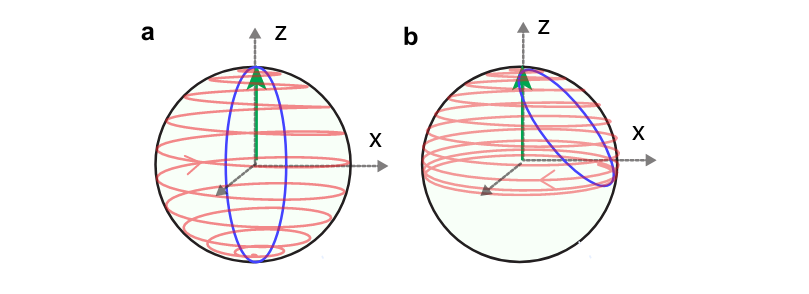
\includegraphics[width=\textwidth]{images/rabi_RWA.png}
    \caption{La linea rossa (blu) rappresenta l'evoluzione di un qubit guidato nel sistema del laboratorio (sistema rotante del drive). \textbf{a} con $\Delta=0$ e \textbf{b} per $\Delta \neq 0$. \url{https://arxiv.org/pdf/1904.09291.pdf}}
    \label{fig:my_label}
\end{figure}

\subsection{Controllo XY}
Consideriamo ora l'hamiltoniana per un qubit TRANSMON accoppiato tramite una capacità a una sorgente che porta un termine dipendente da $\sigma_y$ tale che:
\begin{equation*}
    \hat H= - \hbar \frac{\omega_q}{2}\hat \sigma_z + A(t) \hat \sigma_y
\end{equation*}
Passo al sistema di riferimento in rotazione con $\hat U = e^{-\frac{i}{\hbar}\omega_q t}$.
In questo sistema potrò applicare rotazioni sia rispetto all'asse x che rispetto all'asse y.
L'hamiltoniana si potrà scrivere come:
\begin{equation*}
    \hat H = U H_d U^\dagger = A(t) \left[ \cos \left( \omega_q t \right)\sigma_y -  \sin \left( \omega_q t \right)\sigma_x \right]
\end{equation*}
In questo caso scegliamo $A(t) = A v(t)$ ponendo attenzione non solo sull'ampiezza, ma anche sulla fase:
\begin{equation*}
    v(t) = s(t) \sin \left( \omega_d t + \phi \right)
\end{equation*}
Dove $s(t)$ è una funzione adimensionale che funge da \textit{envelope} e mi porta a poter scrivere l'ampiezza come $As(t)$, mentre la fase $\phi$ è scelta arbitrariamente.
Possiamo riscrivere $v(t)$ come:
\begin{equation*}
    v(t) = s(t) \left( \cos (\phi) \sin (\omega_d t) + \sin (\phi) \cos (\omega_d t) \right)
\end{equation*}
La notazione più in voga per questi termini (che riconosciamo essere le due quadrature del segnale RF) ci dice:
\begin{align*}
    I &= \cos \phi \qquad \text{chiamata per ragioni storiche: componente in fase} \\
    Q &= \sin \phi \qquad \text{chiamata per ragioni storiche: componente fuori fase} 
\end{align*}
E abbiamo le proprietà:
\begin{equation*}
    Q^2 + I^2 = 1 \qquad , \qquad \phi = \arctan\frac{Q}{I}
\end{equation*}
E riscriviamo la nostra hamiltoniana come:
\begin{equation*}
    \hat H = As(t) \left[  I \sin (\omega_d t) - Q \cos (\omega_d t)  \right]\times \left[ \cos (\omega_q t) \sigma_y - \sin (\omega_q t) \sigma_x \right]
\end{equation*}
Svolgendo il prodotto, usando un po' di trigonometria e applicando la RWA (rimuovo i termini dipendenti da $\omega_q + \omega_d$) arrivo a:
\begin{equation*}
    \hat H = \frac{1}{2}As(t) \left[ \left(-I \cos ( \Delta t) + Q \sin ( \Delta t) \right) \sigma_x + \left(I\sin ( \Delta t) - Q \cos ( \Delta t)  \right) \sigma_y \right] 
\end{equation*}
Che, espressa in forma matriciale, diventa:
\begin{equation*}
    \hat H = -\frac{A}{2}s(t) \begin{pmatrix} 0 & e^{i (\Delta t + \phi)} \\ e^{-i (\Delta t + \phi)} & 0 \end{pmatrix}
\end{equation*}
    %%%%%%%%%%%%%%
% LECTURE 17 %
%%%%%%%%%%%%%%
\vspace{1cm}

\noindent\lecture{17}{04/12/2021}

\vspace{0.5cm}

\noindent Riprendiamo il discorso che stavamo affrontando la volta scorsa. L'hamiltoniana $\tilde{H}$ in RWA è indipendente dal tempo, perciò l'evoluzione temporale dello stato generico ruotato è molto semplice
\begin{equation}\label{to_exp_H_tilde}
    \ket{\tilde{\psi}(t)} = e^{-i \tilde{H} t} \ket{\tilde{\psi}(0)} \, .
\end{equation}
In realtà avremmo potuto fin dall'inizio scrivere l'evoluzione temporale dello stato $\ket{\psi (t)}$ non ruotato, utilizzando l'hamiltoniana \eqref{H_no_approx}: abbiamo deciso di non intraprendere quella strada poiché l'espressione dell'operatore unitario che descrive l'evoluzione temporale per $H$ dipendenti dal tempo è abbastanza complicata. 

\noindent Dato che ci serve nella \eqref{to_exp_H_tilde} l'esponenziazione di $\tilde{H}$, esplicitiamo in \eqref{H_tild_RWA} le matrici $\sigma_1$ e $\sigma_2$ (da $\sigma_+$ e $\sigma_-$) e riscriviamo gli esponenziali in termini di seno e coseno: in questo modo otteniamo la seguente combinazione lineare di matrici di Pauli
\begin{equation*}
    \tilde{H} = - \frac{1}{2} \left( \Delta \sigma_3 + A \cos \phi \sigma_1 - A \sin \phi \sigma_2 \right) \equiv -\frac{\Omega}{2} \vec n \cdot \vec \sigma \, ,
\end{equation*}
dove 
\begin{equation}\label{n_dir}
    \vec n = \frac{1}{\Omega} (A \cos \phi, - A \sin \phi, \Delta) \quad \text{con} \quad \Omega = \sqrt{A^2 + \Delta^2} \, ;
\end{equation}
si noti che $\vec n$ è correttamente normalizzato dimodoché $\abs{\vec n} = 1$. La frequenza $\Omega$ è chiamata \textbf{frequenza di Rabi}\footnote{Molti libri usano differenti convenzioni sul significato di tale frequenza. Indipendentemente da ciò, la cosa importante è che l'oscillazione del qubit è controllata da $\Omega$.} e controlla l'oscillazione del qubit. Quindi l'operatore di evoluzione temporale diventa 
\begin{equation}\label{rotation_Omega}
    e^{-i \tilde{H} t} = e^{i \frac{\Omega}{2} \vec n \cdot \vec \sigma t} \, ;
\end{equation}
(la presenza del fattore $1/2$ è comune quando sono presenti le matrici di Pauli). La relazione precedente è esattamente analoga all'operatore \eqref{rotation_n_lambda}, introdotto nella Sezione \ref{sec:gate} riguardante i gate agenti su singoli qubit: la più generale matrice unitaria $2 \times 2$ (a meno di una fase globale) può essere infatti scritta proprio come l'operatore $R_{\vec n}(\gamma)$, ossia
\begin{equation*}
    R_{\vec{n}}(\gamma) = e^{-i \frac{\gamma}{2} (\vec n \cdot \vec \sigma)} \, .
\end{equation*}
Questo operatore va interpretato come una rotazione del qubit lungo la sfera di Bloch: l'evoluzione temporale $R_{\vec n}(- \Omega t)$ effettua una rotazione di angolo $-\Omega t$ attorno alla direzione individuata dal vettore $\vec n$ scritto in precedenza. È bene notare che la direzione attorno a cui avviene questa precessione è specificata dai parametri che individuano i dettagli dell'interazione con la radiazione esterna oscillante, come $\omega_d$, $A$ e $\phi$, ma anche dalla frequenza di oscillazione del qubit stesso ($\omega_q$).  

\noindent Prima di dare uno sguardo concreto alla sfera di Bloch, ricordiamo che per scrivere l'esponenziale di una combinazione lineare di matrici di Pauli è possibile usare la seguente formula:
\begin{equation}\label{formula_for_Rabi}
    R_{\vec{n}}(\gamma) = e^{-i \frac{\gamma}{2} (\vec n \cdot \vec \sigma)} = \mathbb{I} \cos \! \left( \frac{\gamma}{2} \right) - i \sin \! \left( \frac{\gamma}{2} \right) \left( \vec \sigma \cdot \vec n \right) \, .
\end{equation}

\begin{proof}
    Ricordando la serie dell'esponenziale, la proprietà $(\vec \sigma \cdot \vec n)^2 = \mathbb{I}$ e la serie di seno e coseno avremo:
    \begin{align*}
        R_{\vec{n}}(\gamma) &= \sum_{k=0}^\infty \frac{1}{k!} \left( -\frac{i}{2} \gamma \vec n \cdot \vec \sigma \right)^k \\
        &= \sum_{k=0}^\infty \frac{1}{(2k)!} \left( -\frac{i}{2} \gamma \vec n \cdot \vec \sigma \right)^{2k} + \sum_{k=0}^\infty \frac{1}{(2k + 1)!} \left( -\frac{i}{2} \gamma \vec n \cdot \vec \sigma \right)^{2k+1} \\
        &= \mathbb{I} \sum_{k=0}^\infty \frac{(i)^{2k}}{(2k)!} \left( \frac{\gamma}{2} \right)^{2k} -i (\vec n \cdot \vec \sigma) \sum_{k=0}^\infty \frac{(i)^{2k}}{(2k+1)!} \left( \frac{\gamma}{2} \right)^{2k+1} \\
        &= \mathbb{I} \cos \! \left( \frac{\gamma}{2} \right) - i \sin \! \left( \frac{\gamma}{2} \right) \left( \vec \sigma \cdot \vec n \right) \, .
    \end{align*}
\end{proof}

\noindent La \eqref{formula_for_Rabi} è molto utile quando si vogliono affrontare dei conti espliciti. Vediamo per esempio un caso di un esercizio molto semplice in QM:

\begin{esempio}[\textbf{Oscillazioni di Rabi}]
    Supponiamo che il sistema si trovi nello stato iniziale $| \tilde{\psi}(0) \rangle = \ket{0}$ e calcoliamo la probabilità che al tempo $t$ il qubit subisca una transizione $\ket{0} \to \ket{1}$. Ricordando l'espressione \eqref{rotation_Omega} e la formula appena dimostrata avremo
    \begin{equation*}
        P(t)_{0 \to 1} = \abs{\mel{1}{e^{-i \tilde{H} t}}{0}}^2 = \abs{\mel{1}{\cos \! \left( \frac{\Omega}{2} t \right) + i \sin \! \left( \frac{\Omega}{2} t \right) \vec \sigma \cdot \vec n }{0}}^2 \, ;
    \end{equation*}
    il primo termine è nullo, mentre il secondo, ricordando che $\sigma_1 \ket{0} = \ket{1}$ e $\sigma_2 \ket{0} = i \ket{1}$, riceve contributi solamente da $\sigma_1$ e $\sigma_2$. In questo modo possiamo scrivere 
    \begin{align*}
        P(t)_{0 \to 1} &= \abs{i \sin \! \left( \frac{\Omega}{2} t \right) (n_1 + i n_2)}^2 \\
        &= \abs{i \sin \! \left( \frac{\Omega}{2} t \right) \frac{A}{\Omega} e^{-i \phi}}^2 \\
        &= \frac{A^2}{\Omega^2} \sin^2 \! \left( \frac{\Omega}{2} t \right) \, ,
    \end{align*}
    dove nella seconda riga abbiamo usato le componenti di $\vec n$ in \eqref{n_dir}. Inserendo infine l'espressione di $\Omega$ otteniamo la cosiddetta \textbf{formula di Rabi}
    \begin{equation}\label{Rabi_formula}
        P(t)_{0 \to 1} = \frac{A^2}{A^2+\Delta^2} \sin^2 \! \left( \frac{\sqrt{A^2+\Delta^2}}{2} t \right) \, .
    \end{equation}
    
    \begin{figure}[!hb]
    \centering
    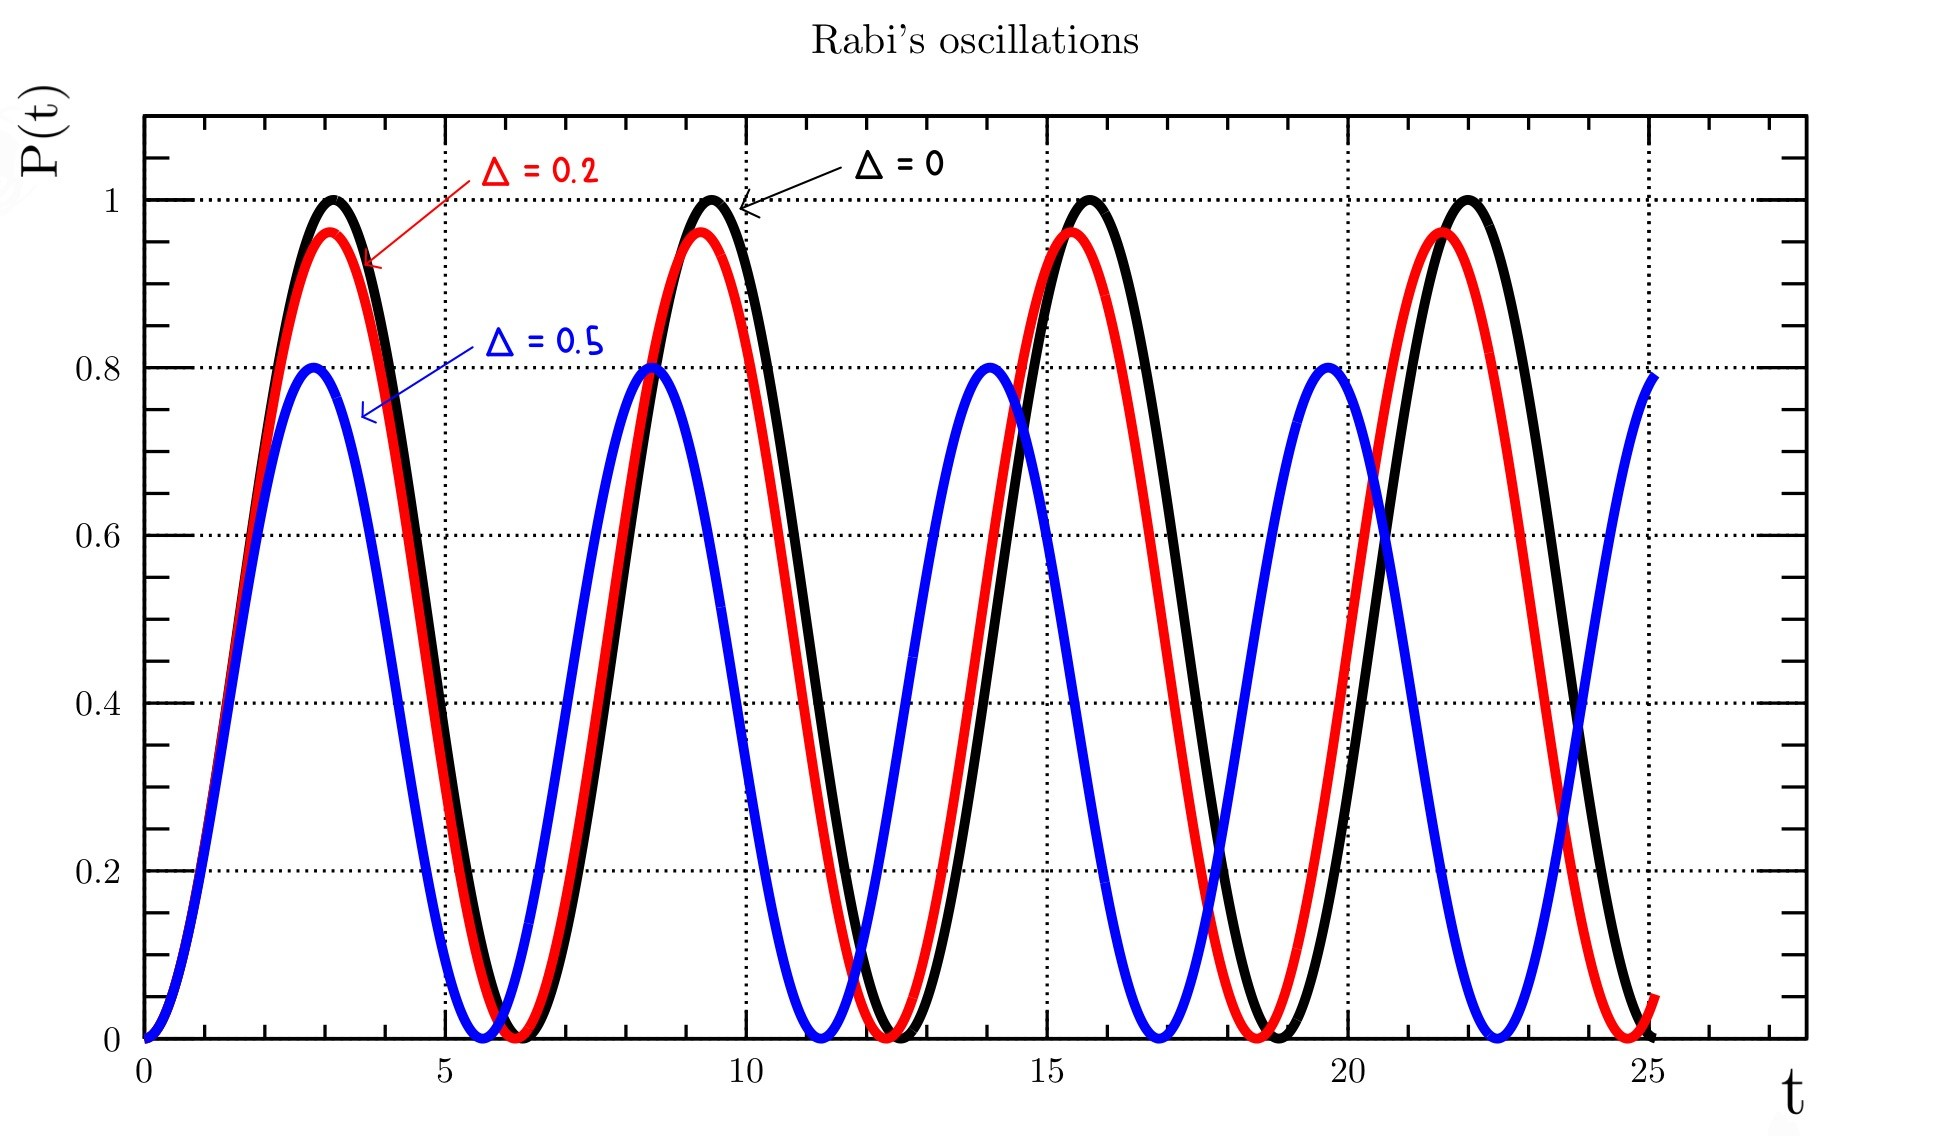
\includegraphics[scale=0.302]{images/Rabi.jpg}
    \caption{Oscillazioni di Rabi per $A = 1$. È evidente come la probabilità del sistema oscilli allo scorrere del tempo. Più il sistema è vicino alla risonanza ($\Delta = 0$), più vicino ad 1 saranno i picchi e quindi maggiore sarà la probabilità di trovare il sistema in $\ket{1}$.}
    \label{fig:Rabi}
    \end{figure}
    
    \noindent Ricapitolando, la \eqref{Rabi_formula} ci fornisce la probabilità al tempo $t$ che applicando una perturbazione esterna oscillante con frequenza $\omega_d$, ampiezza $A$ e detuning $\Delta$ avvenga una transizione $\ket{0} \to \ket{1}$. Si tratta di un risultato molto importante e spesso presente in diversi rami della fisica. 
    
    \noindent Facendo un grafico della probabilità \eqref{Rabi_formula} in funzione del tempo si ottiene la Figura \ref{fig:Rabi}. 
\end{esempio} 

\noindent Cerchiamo ora di visualizzare che cosa accade dal punto di vista della sfera di Bloch. Ricordando la \eqref{rotation_RWA} possiamo scrivere lo stato non ruotato come
\begin{equation*}
    \ket{\psi(t)} = U^\dag (t) \ket{\tilde{\psi}(t)} \, , \quad \text{dove} \quad U^\dag (t) = e^{\frac{i}{2} \omega_d \sigma_3 t} \, ,
\end{equation*}
in questo modo, inserendo anche la \eqref{to_exp_H_tilde}, possiamo scrivere l'evoluzione temporale dello stato non ruotato
\begin{equation}\label{te_non_rotated}
    \ket{\psi(t)} = e^{\frac{i}{2} \omega_d \sigma_3 t} R_{\vec n}(- \Omega t) \ket{\tilde{\psi}(0)} \, .
\end{equation}
Come già anticipato (vedi Figura \ref{subfig:Bloch_Rabi1}), l'operatore $R_{\vec n}(-\Omega t)$ implementa una rotazione di angolo $-\Omega t$ attorno alla direzione di $\vec n$. Per esempio

\begin{esempio}[\textbf{Rotazione attorno a $z$}]
    Supponiamo una rotazione lungo $z$ implementata dall'operatore $R_z(\gamma) = e^{-\frac{i}{2} \sigma_3 \gamma}$. Ricordando la generica parametrizzazione del qubit in \eqref{generic qubit} avremo
    \begin{align*}
        R_z(\gamma) \ket{\psi} &= \cos \! \left( \frac{\theta}{2} \right) e^{-\frac{i}{2} \gamma} \ket{0} + \sin \! \left( \frac{\theta}{2} \right) e^{\frac{i}{2} \gamma} e^{i \phi} \ket{1} \\
        &= e^{-\frac{i}{2} \gamma} \left[ \cos \! \left( \frac{\theta}{2} \right) \ket{0} + \sin \! \left( \frac{\theta}{2} \right) e^{i(\phi + \gamma)} \ket{1} \right] \, ;
    \end{align*}
    riassorbendo la fase globale abbiamo effettivamente ottenuto che l'operatore $R_{\vec n}(\gamma)$ produce una rotazione lungo $z$ perché il qubit finale è dello stesso tipo di quello iniziale con $\theta \to \theta$ e $\phi \to \phi + \gamma$. 
\end{esempio}

\noindent Che cosa accade per una rotazione lungo una generica direzione $\vec n$? La direzione dipende da $(A, \Omega, \phi)$, quindi per rilevarla sperimentalmente basta variare questi parametri. 

\noindent La situazione in cui $A = 0$ (assenza di una perturbazione  esterna) è abbastanza curiosa: in una tale situazione si potrebbe pensare $R_{\vec n} (- \Omega t) = \mathbb{I}$, quindi sembrerebbe dalla \eqref{te_non_rotated} che rimanga un termine $e^{\frac{i}{2} \omega_d \sigma_3 t}$ di rotazione lungo $z$. In realtà questo risultato è sbagliato perché, quando non c'è alcun campo oscillante, è necessario porre $\omega_d = 0$: dalla \eqref{n_dir} il vettore $\vec n$ non è zero, ma bensì $\vec n = (0, 0, \Delta/\Omega)$, perciò
\begin{equation*}
    R_{\vec n} (-\Omega t) = e^{\frac{i}{2} \Delta \sigma_3 t} = e^{\frac{i}{2} (\omega_q - \omega_d) \sigma_3 t} \, ; 
\end{equation*}
questo significa che lo stato continua a subire una precessione
\begin{equation*}
    \ket{\psi(t)} = e^{\frac{i}{2} \omega_d \sigma_3 t} e^{\frac{i}{2} (\omega_q - \omega_d) \sigma_3 t} \ket{\tilde{\psi}(0)} = e^{\frac{i}{2} \omega_q \sigma_3 t} \ket{\tilde{\psi}(0)} \, .
\end{equation*}
Esiste sempre una precessione lungo $z$ con la frequenza naturale del qubit! Delle volte è utile sbarazzarsi di questa precessione cambiando sistema di coordinate: ad esempio possiamo andare in un sistema di riferimento che ruota come il qubit scegliendo $U(t) = e^{i H_0 t}$; in questo modo è possibile tenere solamente la parte non banale dell'evoluzione temporale eliminando questo effetto di precessione. Spesso il sistema di riferimento scelto dipende da ciò che si vuole fare. 

\begin{figure}[!ht]
	\centering	
	\subfloat[][\label{subfig:Bloch_Rabi1} ]{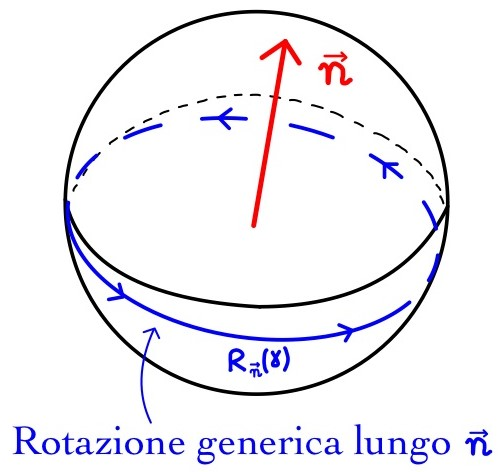
\includegraphics[scale=.4,keepaspectratio]{images/Bloch_Rabi1}} \\
	\subfloat[][\label{subfig:Bloch_Rabi2} ]{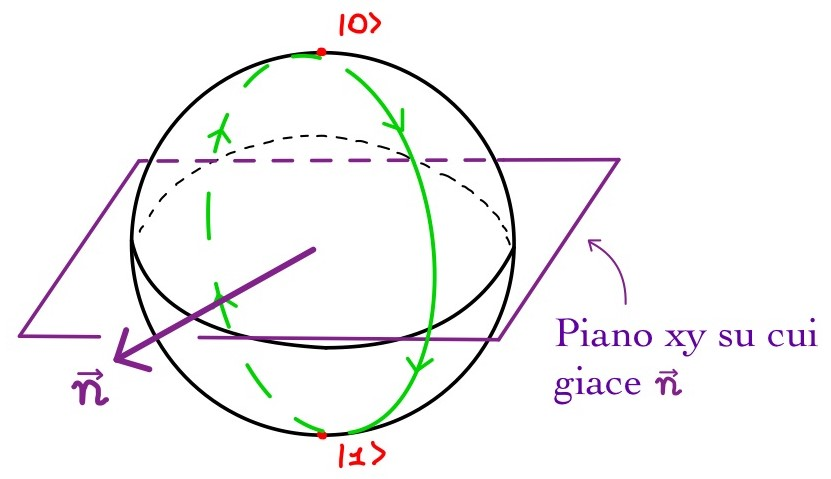
\includegraphics[scale=.4,keepaspectratio]{images/Bloch_Rabi2}} \\
	\subfloat[][\label{subfig:Bloch_Rabi3} ]{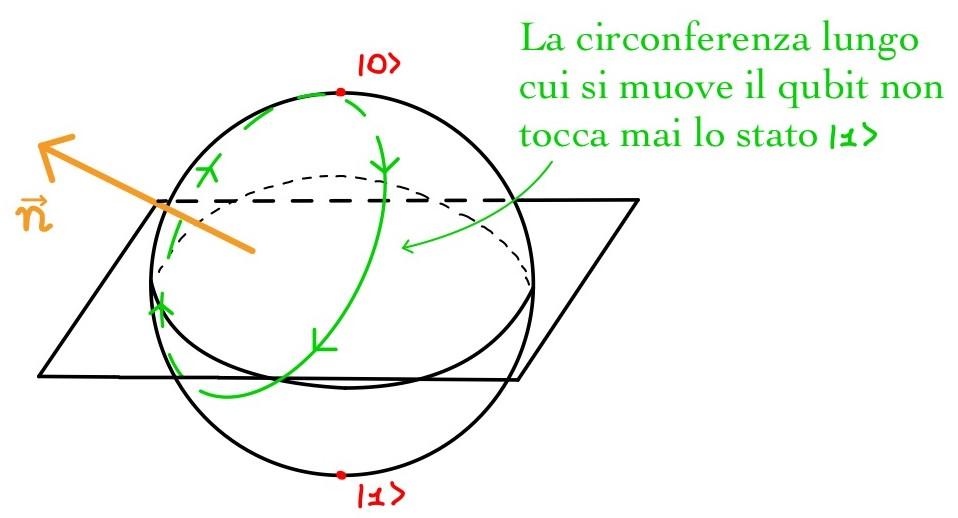
\includegraphics[scale=.4,keepaspectratio]{images/Bloch_Rabi3}}
	\caption{(\ref{subfig:Bloch_Rabi1}) L'operatore $R_{\vec n}(\gamma)$ implementa una generica rotazione attorno ad $\vec n$ lungo la superficie della sfera di Bloch. (\ref{subfig:Bloch_Rabi2}) Alla risonanza, $\vec n$ giace nel piano $xy$, quindi per determinati tempi vi è la certezza che il qubit si trovi in $\ket{1}$. (\ref{subfig:Bloch_Rabi3}) Per $\vec n$ generico non si ha mai la certezza che il qubit si trovi in $\ket{1}$.}
    \label{fig:Bloch_Rabi}
\end{figure}

\noindent Per capire meglio il significato della rotazione di Figura \ref{subfig:Bloch_Rabi1} immaginiamo che il qubit parta nello stato $\ket{0}$. In regime di risonanza ($\Delta = 0$) avremo $\vec n = (\cos \phi, - \sin \phi, 0)$, perciò l'asse di rotazione giace nel piano $xy$ (si consideri la Figura \ref{subfig:Bloch_Rabi2}): geometricamente, il qubit ruota con frequenza $\Omega$ lungo la circonferenza evidenziata in verde, ossia nel piano perpendicolare ad $\vec n$, andando continuamente avanti e indietro da $\ket{0}$ ad $\ket{1}$ (si pensi alla probabilità di Figura \ref{fig:Rabi}). Ci saranno tempi particolari in cui il qubit si trover\`a con certezza in $\ket{1}$.

\noindent Per quale ragione invece per $\Delta \neq 0$ la probabilità non è mai 1? Dalle relazioni \eqref{n_dir}, il vettore $\vec n$ presenta 3 componenti non nulle per $\Delta \neq 0$ quindi, partendo da $\ket{0}$, la circonferenza lungo la quale il qubit si muove non raggiunge mai $\ket{1}$! (si pensi alla Figura \ref{subfig:Bloch_Rabi3}). Ovviamente dalle leggi della QM sappiamo che ci sarà sempre della probabilità che la misura restituisca $\ket{1}$, tuttavia per nessun tempo si avrà la certezza che il qubit si trovi in quello stato. Dal punto di vista pratico è possibile utilizzare questa perturbazione esterna oscillante per muovere arbitrariamente il qubit sulla sfera di Bloch e invertire lo stato dimodoché oscilli continuamente $\ket{0} \leftrightarrow \ket{1}$. 

\noindent Cosa succede quando la perturbazione non è periodica? Una tale situazione è parametrizzata da un campo esterno proporzionale a $f(t) \cos (\omega_d t + \phi_0)$, dove $f(t)$ è un'opportuna funzione dipendente dal tempo. Per svolgere dei conti espliciti è necessario utilizzare il formalismo della teoria delle perturbazioni dipendenti dal tempo: il punto fondamentale è che la fisica rimane la stessa! L'oscillazione è modulata da $f(t)$ perciò è sempre possibile scegliere opportunamente questa funzione e le frequenze in maniera tale che si abbia una situazione in cui, per un dato tempo $t$, il qubit si ritrovi con certezza in $\ket{1}$; in questo modo il tempo può essere scelto arbitrariamente per manipolare il qubit a piacimento. 










\section{Accoppiamento qubit - cavità QED}\label{sec:int_qubit_CQED}
L'accoppiamento di un qubit con un campo elettromagnetico (classico) esterno oscillante può essere essenzialmente utilizzato per creare tutti i gate agenti sui singoli qubit. I gate agenti su più qubit (quelli che creano entanglement tra stati), invece, sono più complessi da realizzare: alcuni di essi possono essere costruiti a partire da situazioni simili a quelle studiate nella scorsa sezione, tuttavia la maggior parte sono realizzati tramite l'accoppiamento di un qubit con un campo elettromagnetico quantizzato. Cerchiamo di approfondire questo discorso. 

\noindent L'elettrodinamica quantistica della cavità (\textbf{Cavity QED}) è un campo di studio che si focalizza su un regime che coinvolge l'accoppiamento di singoli atomi con solo alcuni (pochi) modi ottici. Sperimentalmente, ciò è reso possibile collocando singoli atomi all'interno di cavità ottiche. Poiché all'interno della cavità esistono solo uno o due modi elettromagnetici, e ciascuno di questi ha un'intensità di campo elettrico molto elevata, l'accoppiamento tra il dipolo dell'atomo e il campo è molto intenso. I due principali componenti sperimentali di un sistema QED a cavità sono la cavità elettromagnetica e l'atomo; quest'ultimo, il quale modellizza il qubit, interagisce con alcuni fotoni della cavità, perciò è evidente che dobbiamo considerare un'hamiltoniana che coinvolge una radiazione quantizzata. 

\noindent Nel contesto dell'ottica quantistica si costruisce un tale sistema considerando una cavità Fabry-Perot costituità da una serie di specchi che permettono di intrappolare dei fotoni: il campo elettromagnetico che si genera dalle riflessioni dei fotoni sugli specchi è molto intenso, ma si riescono a selezionare alcuni modi di frequenza $\omega_c$ (pedice $c$ per cavità) ben precisi (o multipli di tale frequenza). Un sistema di questo tipo diventa molto simile alla radiazione di corpo nero perché l'atomo (qubit) nella cavità QED può scambiare e riassorbire fotoni se la frequenza del qubit è simile a quella della cavità, ossia $\omega_q \sim \omega_c$. In generale se i fotoni non possono uscire e l'atomo assorbe alcuni di essi con frequenze ben precise, allora il sistema necessita una completa trattazione in QM. Ovviamente i fotoni possono uscire attraverso delle emissioni spontanee (ricordiamo che c'è sempre qualche perdita e decoerenza).

\noindent L'hamiltoniana totale del sistema, il quale è costituito dal qubit e dalla cavità, sarà descritta da
\begin{equation}\label{eq:ham-cav-qub-free}
    \hat H_0 = -\frac 12 \omega_q\hat \sigma_3+\omega_c\left(\hat a^\dagger \hat a +\frac 12\right) \, ,
\end{equation}
dove in questo caso, nel secondo termine, stiamo descrivendo un solo modo ottico perché nella maggior parte delle situazioni se ne riescono ad eccitare molto pochi; avendo un unico modo del campo e.m. allora, nella trattazione che segue, assumeremo che l'eccitazione dei fotoni coinvolgerà sempre fotoni dello stesso modo ottico dato dagli operatori $\hat{a}$ e $\hat{a}^\dag$. L'hamiltoniana precedente non è nient'altro che l'hamiltoniana libera che descrive contemporaneamente e indipendentemente il qubit e la cavità. Per descrivere la parte interagente del sistema assumiamo un'interazione con il dipolo dell'atomo, quindi introduciamo l'hamiltoniana
\begin{equation}\label{eq:ham-cav-qub-int}
    \hat H_I=\vec d \cdot \vec E \, ,
\end{equation}
dove $\vec d$ dipende dalle interazioni concrete che hanno luogo\footnote{Questo vettore è la posizione se il qubit è costruito da un atomo, altrimenti è lo spin se il qubit è realizzato da un sistema con spin. Similmente, il campo è elettrico nel primo caso, altrimenti è magnetico per l'accoppiamento con lo spin.}, ma allo stesso tempo fornisce i generici elementi di matrice per le transizioni $\ket 0 \rightarrow \ket 1$ e $\ket 1 \rightarrow \ket 0$; $\vec E$ è ovviamente il campo elettrico. Dato che il campo è quantizzato possiamo utilizzare il risultato ottenuto alla fine della Sezione \ref{sec:quantized_em}, cioè
\begin{equation}\label{eq:em-quant.}
    \hat{\vec E} = \vec E_0\left(\hat a e^{i\vec k \cdot \vec x - i \omega t} + \hat a^\dagger e^{-i\vec k \cdot \vec x + i \omega t}\right) \, .
\end{equation}
Diamo uno sguardo alla relazione \eqref{eq:em-quant.}, in particolar modo alla dipendenza spaziale e temporale. Per quanto riguarda la prima, usando l'approssimazione di dipolo, se consideriamo per i fotoni lunghezze d'onda grandi\footnote{Tipicamente la lunghezza d'onda dei fotoni non è così lontana dalla lunghezza d'onda di risonanza del qubit, la quale rimane comunque molto più grande delle dimensioni atomiche.} rispetto alle dimensioni atomiche del sistema, possiamo trascurare la dipendenza spaziale. Un discorso analogo può essere fatto anche per la dipendenza temporale: nel momento in cui si va a quantizzare il campo e.m. di un sistema che assumiamo isolato, l'hamiltoniana che si realizza è solitamente indipendente dal tempo e quindi può essere costruita rispetto a un certo riferimento temporale che, per semplicità, facciamo coincidere con $t=0$. Sotto queste due assunzioni, la \eqref{eq:em-quant.} può essere riscritta come
\begin{equation*}
    \hat{\vec E} = \vec E_0\left(\hat a + \hat a^\dagger\right) \, .
\end{equation*}
Inserendo questo risultato nella \eqref{eq:ham-cav-qub-int} avremo che 
\begin{equation}\label{eq:ham-cav-qub-int2}
    \hat H_I=g\hat\sigma_1\left(\hat a + \hat a^\dagger\right)\, ,
\end{equation}
dove $g$ è la costante di accoppiamento dell'interazione tra il qubit e la radiazione e, anziché prendere gli elementi di matrice dell'operatore $\vec d$ tra gli stati dei qubit (dipendono da molti fattori, come ad esempio i livelli energetici che scegliamo dalle regole di selezione), consideriamo una generica matrice hermitana $2 \times 2$ che, come sappiamo, può essere scritta in termini di una combinazione lineare delle matrici di Pauli. 
Tra tutte le possibili scelte prendiamo, senza perdita in generalità, $\hat \sigma_1$. Ovviamente possiamo fare scelte diverse, come ad esempio $\hat{\sigma_2}$, ma ogni opzione darà sempre un risultato fisico simile.

\noindent A questo punto possiamo mettere insieme la \eqref{eq:ham-cav-qub-free} e la \eqref{eq:ham-cav-qub-int2} per scrivere l'hamiltoniana completa del sistema
\begin{equation}\label{H_da_riscrivere_4}
    \hat H = -\frac 12 \omega_q\hat \sigma_3+\omega_c\left(\hat a^\dagger \hat a +\frac 12\right) + g\hat\sigma_1\left(\hat a + \hat a^\dagger\right) \, ;
\end{equation}
sottolineiamo nuovamente che la differenza principale rispetto al caso della sezione precedente è che qui il campo elettrico è quantizzato, cosa che si riflette con la presenza degli operatori $\hat{a}$ e $\hat{a}^\dag$.

\noindent Ancora una volta, scriviamo $\hat{\sigma}_1$ usando le definizioni di $\hat \sigma_+$ e $\hat \sigma_-$ in \eqref{sigma_+_-}: è evidente che $\hat \sigma_+ \ket{1} = \ket{0}$ e $\hat \sigma_- \ket{0} = \ket{1}$, quindi la prima matrice agisce come operatore di abbassamento sullo stato del qubit, ossia  $\ket{1} \to \ket{0}$, mentre la seconda come operatore di innalzamento $\ket{0} \to \ket{1}$. Se scriviamo $\hat\sigma_1 = \hat\sigma_++\hat\sigma_-$ e ci concentriamo sul solo termine di interazione, avremo quindi
\begin{equation}\label{H_interaz_4}
    \hat H_I = g\big(
    \underbrace{\hat \sigma_+\hat a^\dagger}_{1.}+
    \underbrace{\hat\sigma_-\hat a}_{2.}+
    \underbrace{\hat\sigma_+\hat a}_{3.}+
    \underbrace{\hat\sigma_-\hat a^\dagger}_{4.}
    \big)\, ;
\end{equation}
quale è l'interpretazione di ciascuno di questi 4 termini sottolineati? Tenendo presente che $\hat{a}$ distrugge un fotone, $\hat{a}^\dag$ crea un fotone e che abbiamo posto $\hbar \omega_q = E_1 - E_0$, il loro significato sarà:
\begin{enumerate}
    \item Il qubit emette un fotone e di conseguenza lo stato energetico si diseccita;
    \item Il qubit assorbe un fotone e di conseguenza lo stato energetico si eccita;
    \item Assorbimento di un fotone e diseccitazione del qubit: viene fornita energia $2 \omega_q$;
    \item Emissione di un fotone ed eccitazione del qubit: viene rimossa energia $-2 \omega_q$.
\end{enumerate}
Gli ultimi due processi sono abbastanza insoliti, anche se potrebbero verificarsi se il sistema possiede energia a sufficienza. In teoria delle perturbazioni al primo ordine solamente i primi due processi sono permessi, mentre gli ultimi due sono vietati dalla regola d'oro di Fermi, perciò, anche in una trattazione esatta, hanno una probabilità molto piccola di verificarsi. Possiamo quindi assumere che i primi due termini siano permessi (più probabili) quando siamo vicini alla risonanza, mentre gli ultimi sono soppressi in teoria delle perturbazioni perché hanno una piccola probabilità che accadano: dunque, a meno che $\omega_c$ e $\omega_q$ non siano troppo lontani tra loro, possiamo trascurare gli ultimi due processi. 

\noindent Verifichiamo quanto detto, ancora una volta, con la RWA, ma questa volta prendiamo una strada leggermente diversa perché è più conveniente scegliere
\begin{equation*}
    \hat U(t) = e^{i\hat H_0 t} \, ,
\end{equation*}
dove $\hat H_0$ non è nient'altro che l'hamiltoniana della \eqref{eq:ham-cav-qub-free} (questa è nota come \textit{rappresentazione di interazione} in teoria delle perturbazioni). Vediamo come cambia la nuova hamiltoniana a seguito dell'azione $\hat U$: se usiamo la \eqref{S_eq_rotated_state} allora è facile vedere che la scelta precedente ci permette di cancellare il termine libero, infatti
\begin{equation*}
    \hat{\tilde{H}} = \hat U \hat H \hat U^\dagger + i\dot{\hat U}\hat U^\dagger=\hat H_0 + \hat U \hat H_I \hat U^\dagger - \hat H_0= \hat U \hat H_I \hat U^\dagger \, .
\end{equation*}
Per calcolare la coniugazione dell'hamiltoniana \eqref{H_interaz_4} è necessario fare uso del Lemma \ref{lemma:lemma_ops}. Ricordando le seguenti regole di commutazione
\begin{align*}
    \comm{\hat H_0}{\hat a^\dagger} &= \omega_c \hat a^\dagger \, , 
    &\comm{\hat H_0}{\hat \sigma_+} &= -\omega_q\hat \sigma_+ \, , \\
    \comm{\hat H_0}{\hat a} &= -\omega_c \hat a \, , &\comm{\hat H_0}{\hat \sigma_-} &= \omega_q\hat \sigma_- \, ,
\end{align*}
possiamo facilmente scrivere che
\begin{equation}\label{RWA_ops_trans}
    \begin{aligned}
    e^{i\hat H_0t} \hat a^\dagger e^{-i\hat H_0t} &= e^{i\omega_ct} \hat a^\dagger \, , \qquad
    &e^{i\hat H_0t} \hat \sigma_+ e^{-i\hat H_0t} &= e^{-i\omega_qt} \hat \sigma_+ \, , \\
    e^{i\hat H_0t} \hat a e^{-i\hat H_0t} &= e^{-i\omega_ct} \hat a \, , \qquad
    &e^{i\hat H_0t} \hat \sigma_- e^{-i\hat H_0t} &= e^{i\omega_qt} \hat \sigma_- \, ;
    \end{aligned}
\end{equation}
in questo modo la coniugazione completa diventa
\begin{equation*}
    \hat{\tilde{H}} = g \Big( 
    \underbrace{e^{i(\omega_c - \omega_q)t}}_{\sim 1}\hat \sigma_+\hat a^\dagger +
    \underbrace{e^{-i(\omega_c - \omega_q)t}}_{\sim 1}\hat \sigma_-\hat a +
    \underbrace{e^{-i(\omega_c + \omega_q)t}}_{\sim e^{-2i\omega_qt}}\hat \sigma_+\hat a +
    \underbrace{e^{i(\omega_c + \omega_q)t}}_{\sim e^{2i\omega_qt}}\hat \sigma_-\hat a^\dag
    \Big)
\end{equation*}
dove abbiamo supposto il regime di risonanza $\omega_c \sim \omega_q$. Gli ultimi due termini, dal momento che presentano delle rapide oscillazioni, sono soppressi in teoria delle perturbazioni e possiamo quindi trascurarli nella RWA, proprio come avevamo discusso nella sezione precedente.

\noindent Ritornando infine all'hamiltoniana \eqref{H_da_riscrivere_4} nel sistema di riferimento non ruotato, possiamo trascurare gli ultimi due termini della \eqref{H_interaz_4} e scrivere quindi la cosiddetta \textbf{hamiltoniana di Jaynes-Cummings}:
\begin{equation}\label{eq:ham-jaynes-cummings}
    \hat H = -\frac{\omega_q}{2}\hat \sigma_3 + \omega_c\left(\hat a^\dagger \hat a + \frac 12\right)+g\left(\hat \sigma_+\hat a^\dagger + \hat \sigma_-\hat a\right) \, .
\end{equation}
Si tratta dell'hamiltoniana che descrive il sistema della cavity QED, ossia un qubit interagente con delle oscillazioni descrivibili dal punto di vista quantistico (non necessariamente fotoni). Nelle sezioni successive, quando verrà trattato il sistema della trappola ionica, considereremo dei fononi, ma l'hamiltoniana rimarrà comunque della stessa forma. Di solito anche per i qubit superconduttivi si utilizzano hamiltoniane di questo tipo.
    %%%%%%%%%%%%%%
% LECTURE 18 %
%%%%%%%%%%%%%%

\vspace{1cm}
\noindent\lecture{18}{10/12/2021}
\vspace{0.5cm}

\noindent Abbiamo visto come la CQED\footnote{Abbreviazione per Cavity Quantum Electrodynamics.} modellizzi l'interazione tra un qubit e il campo elettromagnetico quantizzato generato all'interno di una cavità o un risonatore. L'hamiltoniana di Jaynes-Cummings \eqref{eq:ham-jaynes-cummings} fu studiata per la prima volta nel contesto dell'ottica quantistica: non appare solo in questo caso particolare, ma in tutti quei casi in cui un qubit interagisce con uno dei modi quantizzati del campo elettromagnetico, ossia descrive tutte quelle interazioni della forma $\vec d \cdot \vec E$, $\vec \mu \cdot \vec B$, ecc.

\noindent Giunti a questo punto vogliamo discutere il significato fisico che si trova dietro a questa hamiltoniana, in particolare vedremo qualche semplice esempio di codifica di un qubit in un modello CQED. Innanzitutto notiamo che l'hamiltoniana originale non approssimata della relazione \eqref{H_da_riscrivere_4} non poteva essere risolta esattamente, tuttavia grazie alla RWA può essere invece diagonalizzata! 

\noindent Dal punto di vista della QM, l'hamiltoniana \eqref{eq:ham-jaynes-cummings} costituisce un semplice problema di accoppiamento tra spin e oscillatore armonico (le eccitazioni di questo oscillatore sono fotoni). Lo spazio di Hilbert totale è infinito dimensionale in quanto è frutto del prodotto $\mathcal{H}_c \otimes \mathcal{H}_q$, dove $\dim \mathcal{H}_c = \infty$ (infiniti oscillatori). Nonostante ciò, l'hamiltoniana sopra è diagonalizzabile perché è una matrice diagonale a blocchi; per tale ragione suddividiamo gli stati utilizzando la seguente notazione:
\begin{align*}
    &\ket{0} \equiv \ket{g} &\Rightarrow& &&\text{Stato fondamentale del qubit.} \\
    &\ket{1} \equiv \ket{e} &\Rightarrow& &&\text{Stato eccitato del qubit.} \\
    &\ket{n} = \ket{0}, \ket{1}, \ket{2}, \ldots &\Rightarrow& &&\text{Numero di fotoni campo elettromagnetico.}
\end{align*}
La struttura a blocchi è evidente notando che $\ket{e,n} \leftrightarrow \ket{g,n+1}$, ossia sono trasformati l'uno nell'altro dai termini dell'interazione: infatti
\begin{align*}
    \hat a^\dagger \hat \sigma_+ \ket{e,n} &= \sqrt{n+1} \ket{g,n+1} \, , \\
    \hat a \hat \sigma_- \ket{g, n+1} &= \sqrt{n+1} \ket{e,n} \, ,
\end{align*}
perché nel primo caso diseccitiamo lo stato del qubit e creiamo un fotone di diseccitazione (lo stato finale è lo stato fondamentale con un fotone in più), mentre nel secondo caso distruggiamo un fotone della cavità, il quale viene assorbito dallo stato fondamentale, che sarà poi eccitato. Alla luce di questa osservazione possiamo suddividere lo spazio di Hilbert totale $\mathcal{H}$ in
\begin{equation}\label{CQED_states}
    \left\{\ket{g,0}\right\} \, , \quad \left\{ \ket{e,n}, \, \ket{g,n+1}\right\} \, ;
\end{equation}
decomponendo $\mathcal{H}$ in questo modo, ogni qualvolta che si agisce con i termini di interazione in \eqref{eq:ham-jaynes-cummings} si rimane sempre nello stesso sottospazio. Tenendo presente che $\hat{H}_0$ è diagonale, mentre $\hat{H}_I$ è off-diagonal, allora in forma matriciale l'hamiltoniana diventa
\begin{equation*}
    \hat H = \frac 12 \omega_c \mathbb{I} + 
    \begin{pmatrix}
        -\frac{\omega_q}2 & & & \\
        & \begin{pmatrix}
            \omega_c - \frac{\omega_q}2 & g \\
            g & \omega_c + \frac{\omega_q}2
          \end{pmatrix} & & \\
        & & \ddots & \\
        & & & \begin{pmatrix}
            \omega_c(n+1) - \frac{\omega_q}2 & g\sqrt{n+1} \\
            g\sqrt{n+1} & \omega_c n + \frac{\omega_q}2
        \end{pmatrix} \\
    \end{pmatrix}
    \begin{matrix}
        \ket{g,0}\\
        \ket{g,1}\\
        \ket{e,0}\\
        \\
        \ket{g,n+1}\\
        \ket{e,n}
    \end{matrix}\, ,
\end{equation*}
dove il termine iniziale rappresenta l'energia di punto zero, detta \textbf{ZPE} ("Zero Point Energy"). (Gli stati a destra sono per ricordare ciò a cui fanno riferimento i blocchi di questa matrice). Ricordando che il \textbf{detuning} è definito come $\Delta=\omega_q - \omega_c$ e tenendo conto della ZPE, possiamo allora riscrivere il blocco generico (ultimo elemento) della matrice precedente come
\begin{equation*}
    \begin{pmatrix}
        (n+1)\omega_c - \frac{\Delta}2 & \sqrt{n+1}g \\
        \sqrt{n+1}g & (n+1)\omega_c + \frac{\Delta}2
    \end{pmatrix} \, ;
\end{equation*}
diagonalizzando questo blocco, lo spettro dell'hamiltoniana è dato dai seguenti autovalori e autostati
\begin{align*}
    E_+ &= (n+1)\omega_c + \frac 12 \sqrt{\Delta^2+4g^2(n+1)} \, , &\ket{n_+} &= \sin\theta_n \ket{g,n+1} + \cos\theta_n\ket{e,n} \, , \\
    E_- &= (n+1)\omega_c - \frac 12 \sqrt{\Delta^2+4g^2(n+1)} \, , &\ket{n_-} &= \cos\theta_n\ket{g,n+1}-\sin\theta_n\ket{e,n} \, ;
\end{align*} 
ad essi si aggiunge il singolo stato $\ket{g,0}$ con energia $E_0 = - \frac{\Delta}{2}$. Gli stati $\ket{n_-}$ e $\ket{n_+}$ prendono il nome di \textbf{dressed states} e l'angolo $\theta_n$ risulta essere definito come
\begin{equation*}
    \tan {2 \theta_n} = \frac{2g\sqrt{n+1}}{\Delta} \, .
\end{equation*}

\noindent Che cosa succede ad un sistema come questo? L'evoluzione temporale, che ricordiamo essere data da $e^{-i\hat H t}$ (hamiltoniana indipendente dal tempo), realizza delle \textbf{oscillazioni di Rabi} sulla coppia dei \textbf{dressed states}: ogni stato si comporta come un sistema a due livelli che oscilla coerentemente in cicli di assorbimento ed emissione di fotoni in maniera tale che gli stati in \eqref{CQED_states} si trasformino continuamente l'uno nell'altro, ossia $\ket{g,n+1} \leftrightarrow \ket{e,n}$. Confrontando con il caso dei campi esterni, qui abbiamo due accoppiamenti: l'interazione è quantificata da $g$, la forza dell'accoppiamento tra i due sistemi, alla quale si aggiunge però $n$, ovvero il numero dei fotoni. La frequenza di Rabi delle oscillazioni risulta quindi essere data da $\sqrt{\Delta^2+4g^2(n+1)}$: maggiore è il numero di fotoni, più grande sarà la frequenza di oscillazione del qubit.

\noindent In ottica quantistica si è spesso interessati a guardare a situazioni in cui si ha una sovrapposizione di differenti stati con numero di fotoni fissato. In questi contesti l'oscillazione generale è più complicata: ogni insieme di fotoni si accoppia in blocchi di 2 cosicché ogni blocco oscilli a coppie. Il punto fondamentale è che la sovrapposizione di oscillazioni crea una situazione in cui non ci sono oscillazioni! Talvolta è possibile aspettare del tempo a sufficienza fino a quando si ritorna ad osservare un pattern di oscillazioni: tipicamente, quando si sovrappongono molti sistemi oscillatori, si ha interferenza, quindi se si aspetta un tempo sufficiente si possono di nuovo osservare delle oscillazioni (rilevate sperimentalmente).   

\begin{figure}[!ht]
    \centering
    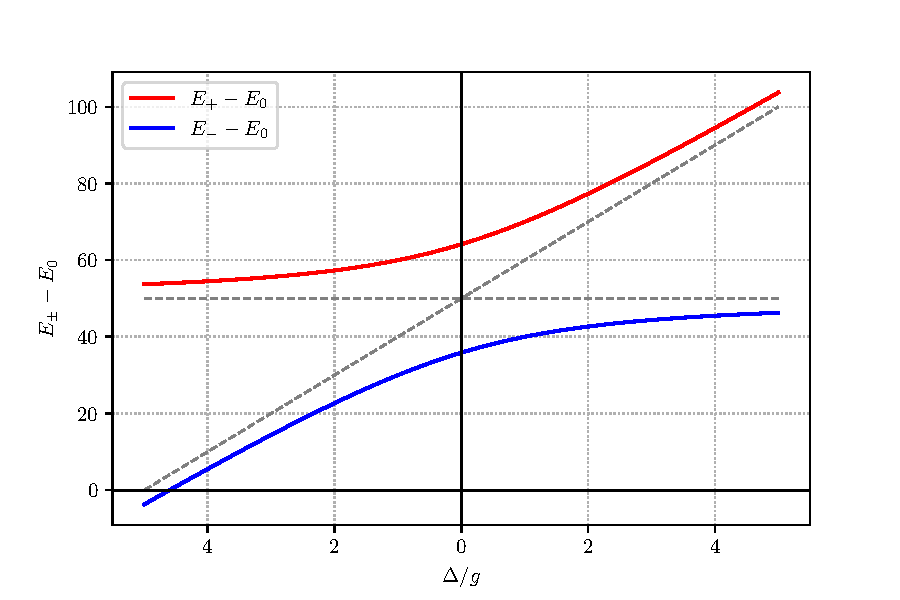
\includegraphics[scale=1]{images/graph.pdf}
    \caption{Differenza in energia dei dressed states con lo stato fondamentale in funzione del detuning. Si noti che la minima differenza di energia tra $E_+$ e $E_-$ si trova in corrispondenza di $\Delta = 0$, mentre la maggior differenza è data quando $\Delta$ diverge. L'asintoto orizzontale si trova in corrispondenza dei limiti: $\lim_{\Delta \to -\infty} (E_+-E_0) = \lim_{\Delta \to +\infty} (E_--E_0) = (n+1) \omega_c$. In questo caso si sono impostati i seguenti valori $\omega_c = 25$, $g=10$, $n=1$.}
    \label{fig:plot-dressed-states-detuning}
\end{figure}

\noindent Nel caso invece del qubit è possibile "giocare" con $g$, $n$ e $\Delta$ per osservare questo pattern di oscillazioni. Nella scorsa sezione abbiamo visto che in una situazione di risonanza esatta ($\Delta = 0$) vi era certezza che ad un certo punto il qubit avesse subito una transizione $\ket{0} \to \ket{1}$. Come vedremo tra poco, in altre situazioni può essere utile considerare il cosiddetto \textbf{regime dispersivo}, ossia $\Delta \neq 0$. Consideriamo l'energia dei \textbf{dressed states} come funzione del \textbf{detuning}: la differenza in energia con lo stato fondamentale non è altro che
\begin{equation*}
    E_\pm - E_0 = (n+1)\omega_c \pm \frac 12\sqrt{\Delta^2+4g^2(n+1)}+\frac \Delta 2 \, ;
\end{equation*}
se disegniamo un plot in funzione di $\frac{\Delta}{g}$ otteniamo la Figura \ref{fig:plot-dressed-states-detuning}. I due regimi particolarmente interessanti sono:
\begin{itemize}
    \item \textbf{Regime di risonanza}, quindi $\Delta = 0$ ($\omega_c=\omega_q$): in questo caso $\theta_n=\frac \pi 4$, per cui $\cos\theta_n=\sin\theta_n=\frac1{\sqrt2}$. Si dice che vi è un'\textbf{ibridizzazione massima} degli stati poiché
    \begin{equation*}
        \ket{n_\pm}= \frac{\ket{g,n+1}\pm\ket{e,n}}{\sqrt 2} \, ;
    \end{equation*}
    essi prendono il nome di \textbf{polarons}. La differenza in energia qui è la minima possibile e dipende da $n$:
    \begin{equation*}
        E_\pm = (n+1)\omega_c \pm g \sqrt{n+1} \, .
    \end{equation*}
    In generale è una situazione abbastanza simile alle oscillazioni di Rabi della Figura \ref{fig:Rabi}.
    
    \item \textbf{Regime dispersivo}, tale che $\Delta \gg g$: qui $\theta_n\ll 1$ e gli stati originali rimangono pressoché invariati a meno di piccole correzioni
    \begin{align*}
        \ket{n_-} &= \ket{g,n+1} + \dots \, , \\
        \ket{n_+} &= \ket{e,n} + \dots \, ;
    \end{align*}
    notiamo che questo comportamento è previsto dato che $\frac{\Delta}{g} \to \infty$ significa equivalentemente che $\Delta = \text{ cost}$ e $g \simeq 0$: siamo vicini al caso libero in cui il qubit e la radiazione e.m. sono quasi disaccoppiati. 

    \noindent Questo regime è interessante per diverse ragioni: ad esempio può essere utile tenere le piccole correzioni negli stati $\ket{n_+}$ e $\ket{n_-}$. Sviluppando la radice in $\frac{g^2}{\Delta^2}$ si ha
    \begin{align*}
        E_\pm &= (n+1)\omega_c \pm \frac 12 \sqrt{\Delta^2+4g^2(n+1)} \\
              &= (n+1)\omega_c \pm \frac{\Delta}{2} \sqrt{1+ \frac{4g^2}{\Delta^2}(n+1)} \\
              &= (n+1)\omega_c \pm \frac{\Delta}{2}\left(1+\frac{2g^2}{\Delta^2}(n+1)+\dots\right) \\
              &= (n+1)\omega_c \pm \left(\frac\Delta 2 +\frac{g^2}{\Delta}(n+1)+\dots\right) \, ;
    \end{align*}
    Osserviamo che possiamo ricavare le medesime energie dando una descrizione efficace del sistema con la seguente hamiltoniana
    \begin{equation}\label{eq:effective-hamiltonian}
        \hat H^{(2)}=\omega_c\left(\hat a^\dagger \hat a + \frac 12\right)-\frac{\omega_q}2\hat \sigma_3 - \frac{g^2}{\Delta}\left(\hat a^\dagger \hat a + \frac 12\right) \hat{\sigma}_3 + \frac{g^2}{2\Delta}\mathbb{I}_{2\times2} \, ,
    \end{equation}
    infatti
    \begin{align*}
        \hat H^{(2)}\ket{g, n+1} &= \omega_c\left(n+1+\frac 12\right)-\frac{\omega_q}{2}-\frac{g^2}{\Delta}(n+1) \\ 
        &= \omega_c(n+1)-\frac{\Delta}2 -\frac{g^2}\Delta(n+1) \equiv E_- \, , \\
        \hat H^{(2)}\ket{e,n} &= \omega_c\left(n+\frac 12\right) + \frac{\omega_q}2 + \frac{g^2}{\Delta}\left(n+ \frac 12\right) + \frac{g^2}{2\Delta} \\
        &= \omega_c(n+1)+\frac{\Delta}2 + \frac{g^2}\Delta(n+1) \equiv E_+ \, .
    \end{align*}
    Dunque possiamo dire che l'hamiltoniana efficace $\hat{H}^{(2)}$ descrive la fisica del sistema nel regime dispersivo. Sui libri si trovano spesso hamiltoniane più complicate: questa hamiltoniana è un esempio della cosiddetta \textbf{trasformazione di Schrieffer-Wolff}. Si tratta di scegliere l'operatore $\hat{U}$ della \eqref{S_eq_rotated_state} indipendente dal tempo e della forma 
    \begin{equation*}
        \hat U = e^{\hat{S}} \, , \quad \text{dove} \quad S^\dag = - S \, .
    \end{equation*}
    L'operatore $\hat{S}$ è scelto in maniera tale che si possa effettuare un'espansione in teoria delle perturbazioni su un opportuno parametro. Se l'hamiltoniana si scrive come $\hat{H} = \hat{H}_0 + \hat{H}_I$, allora si sceglie un $\hat{S}$ tale che $\comm{\hat{S}}{\hat{H}_0} = -\hat{H}_I$. Con un po' di algebra si dimostra che
    \begin{equation*}
        \hat{U} \hat{H} \hat{U}^\dag = \hat{H}_0 + \frac{1}{2} \comm{\hat{S}}{\hat{H}_I} + \order{S^3} \, .
    \end{equation*}
    Nel nostro caso, l'espressione di $\hat H^{(2)}$ si ottiene dall'espansione fino a $\order{g^2/\Delta^2}$ nel sistema ruotato dall'operatore
    \begin{equation*}
        \hat U = e^{-\frac{g}{\Delta}(\hat \sigma_+\hat a^\dagger - \hat \sigma_-\hat a)} \, .
    \end{equation*}
    
    Riscriviamo l'hamiltoniana \eqref{eq:effective-hamiltonian} senza i termini costanti:
    \begin{equation*}
        \hat H^{(2)} = \omega_c  \hat a^\dagger \hat a - \frac{\omega_q}2\hat \sigma_3 - \frac{g^2}{\Delta}\left(\hat a^\dagger \hat a + \frac 12\right) \hat{\sigma}_3 \, .
    \end{equation*}
    A seconda di ciò che si sta facendo è utile raggruppare gli operatori interni a questa espressione in due modi:
    
    \begin{itemize}
        \item Possiamo raggruppare scrivendo 
    \begin{equation*}
        \hat H^{(2)}= \left(\omega_c-\chi\hat \sigma_3\right)\hat a^\dagger \hat a-\frac{\tilde{\omega}_q}{2}\hat \sigma_3 \, ,
    \end{equation*}
    dove $\chi = g^2/\Delta$ e $\tilde{\omega}_q=\omega_q+g^2/\Delta$. È evidente che l'energia della cavità dipenderà da una frequenza che risulta shiftata di una costante $\chi$ dipendente dallo stato del qubit; similmente $\omega_q$ è ridefinito a seguito dell'interazione con il campo elettromagnetico (si parla infatti di \textbf{Lamb shift}, in onore dell'analogo in fisica atomica). Per tale ragione questa situazione può essere utilizzata per realizzare una \textbf{quantum nondemolition measurement}: possiamo stabilire lo stato in cui si trova il qubit misurando la frequenza della cavità! Si noti che questo non viola le leggi della QM.
    
    \item Un modo equivalente è quello di raggruppare tutte le matrici $\hat{\sigma_3}$ scrivendo
    \begin{equation*}
        \hat H^{(2)}= \omega_c\hat a^\dagger \hat a - \frac{\hat \sigma_3}{2}\left(\omega_q + \frac{g^2}{\Delta}+\frac{2g^2}{\Delta}\hat a^\dagger \hat a \right) \, ;
    \end{equation*}
    in questa visione la frequenza del qubit è ridefinita a seguito di due fattori: il Lamb shift (secondo termine della parentesi) e il cosiddetto \textbf{AC - Stark Effect} (ultimo termine), il quale indica il numero di fotoni che creano rumore nella frequenza dei qubit; quindi in questo caso anche il numero di fotoni influenza la frequenza del qubit. 
    \end{itemize}
\end{itemize}

\subsection{Operazioni su 2 qubit}
Il regime dispersivo nel sistema qubit-cavità può essere utilizzato per codificare delle operazioni (gate) che coinvolgono due qubit. Ricordiamo che nella sezione precedente abbiamo visto che le operazioni sui \textbf{singoli} qubit sono realizzate abbastanza semplicemente per mezzo delle oscillazioni di Rabi. Qui il trucco è quello introdurre uno stato addizionale, che chiamiamo $\ket{\gamma}$, al fuori della cavità risonante (in cui sono presenti gli stati $\ket{g}$ e $\ket{e}$ che interagiscono con i fotoni):
\begin{center}
    \mbox{
        \Qcircuit @C=1em @R=2em {
            \lstick{\ket{e}} & \qw & \qw & \qw \\
            \lstick{\ket{g}} & \qw & \qw & \qw
        }
    }
    \raisebox{-1em}{\mbox{
        \Qcircuit @C=1em @R=2em {
            & \qw & \qw & \qw & \rstick{\ket{\gamma}} \\
        }
    }}
\end{center}
Precisiamo che $\ket{e}$ e $\ket{g}$ sono accoppiati con la cavità, mentre $\ket \gamma$ è disaccoppiato dal sistema qubit-cavità. L'idea è quella di codificare un qubit con gli stati $( \ket g, \ket \gamma)$ e uno con gli stati $(\ket 0, \ket 1)$ dei fotoni, cosicché lo spazio di Hilbert totale contenga gli stati seguenti
\begin{equation*}
    \mathcal{H}=\left\{\ket{\gamma 0}, \ket{\gamma 1}, \ket{g0}, \ket{g1}\right\} \, .
\end{equation*}
L'interazione sarà descritta dall'hamiltoniana \eqref{eq:effective-hamiltonian}: lo stato $\ket{e}$ è irrilevante in questa descrizione, mentre l'accoppiamento qubit-cavità è dato dagli ultimi due termini interagenti (quelli con $g$). Consideriamo l'evoluzione temporale del sistema del qubit: gli operatori $\hat{\sigma}_3$ e $\mathbb{I}$ agiscono solamente su $\ket{e}$ e $\ket{g}$ perché $\ket{\gamma}$ è disaccoppiato. Per tale motivo, dal momento che $\hat \sigma_3\ket{\gamma}=\mathbb{I}\ket{\gamma}=0$ e $\hat \sigma_3\ket{g}=\ket{g}$, la parte interagente di $\hat{H}$ agisce come
\begin{equation*}
    e^{-i \hat H_It}=e^{i\frac{g^2}{\Delta}\hat a^\dagger \hat a \hat \sigma_3 t + i\frac{g^2}{2\Delta}(\hat \sigma_3 - \mathbb{I}_{2\times2})t}=\begin{pmatrix}
        1 & & & \\
        & 1 & & \\
        & & 1 & \\
        & & & e^{i\frac{g^2}{\Delta}t}
    \end{pmatrix}
    \begin{matrix}
        \ket{\gamma 0} \\ \ket{\gamma 1} \\ \ket{g 0} \\ \ket{g1}
    \end{matrix} \, .
\end{equation*}
(come in precedenza sono scritti gli stati sulla destra per ricordare l'origine degli elementi di matrice). Il gate risultante è detto \textbf{QPG}, ossia \textbf{Quantum Phase Gate}, poiché è della forma
\begin{equation*}
    Q_\eta = \begin{pmatrix}
        1 & & & \\
        & 1 & & \\
        & & 1 & \\
        & & & e^{i\eta}
    \end{pmatrix} \, .
\end{equation*}
Questa tipologia di gate include il caso $\eta = \pi$, ovvero 
\begin{equation*}
    Q_\pi = \begin{pmatrix}
        1 & & & \\
        & 1 & & \\
        & & 1 & \\
        & & & -1
    \end{pmatrix} \, ;
\end{equation*}
il gate precedente potrebbe sembrare banale ma non lo è perché, usando operazioni a singolo gate su $\ket{\gamma}$, $\ket{g}$, può essere convertito in un \texttt{CZ-gate} (Controlled-$Z$)
\begin{center}
    \mbox{
        \Qcircuit @C=1em @R=1em {
            & \qw & \ctrl{1} & \qw & \qw & \\
            & \qw & \gate{Z} & \qw & \qw &
        }
    }
\end{center}
ma sappiamo che quest'ultimo è legato al \texttt{CNOT-gate} attraverso l'applicazione di due \texttt{H-gate}

\begin{center}
    \mbox{
        \Qcircuit @C=1em @R=1.2em {
            & \qw & \ctrl{1} & \qw & \qw & \\
            & \qw & \targ & \qw & \qw &
        }
    }
    \raisebox{-1em}{=}
    \mbox{
        \Qcircuit @C=1em @R=1em {
            & \qw & \ctrl{1} & \qw & \qw & \\
            & \gate{H} & \gate{Z} & \gate{H} & \qw &
        }
    }
\end{center}
Questo significa che con delle singole operazioni possiamo trasformare un QPG in un \texttt{CNOT-gate}, che sappiamo molto bene che agisce su due qubit contemporaneamente. 

\noindent Cosa succede invece ai termini non interagenti in \eqref{eq:effective-hamiltonian}? Anche loro permettono di implementare delle trasformazioni sui qubit: l'evoluzione temporale dell'hamiltoniana libera è disaccoppiata poiché $\hat{H}^{(2)}_0$ è somma delle hamiltoniane del qubit e della cavità. Perciò questa evoluzione può sempre essere fattorizzata come
\begin{equation*}
    e^{-i\omega_c\left(\hat a^\dagger \hat a + \frac 12\right)t + i\frac{\omega_q}{2}\hat \sigma_3t} = e^{-i\omega_c\left(\hat a^\dagger \hat a + \frac 12\right)t}e^{i\frac{\omega_q}{2}\hat \sigma_3t}=
    e^{-i\frac{\omega_c}{2}t}
    \underbrace{\begin{pmatrix}
        1 & 0\\
        0 & e^{i\frac{\omega_q}{2}t}
    \end{pmatrix}
    }_{\{\ket \gamma, \ket g\}}
    \otimes
    \underbrace{
    \begin{pmatrix}
        1 & 0\\
        0 & e^{i\omega_c t}
    \end{pmatrix}
    }_{\{\ket 0, \ket 1\}} \, .
\end{equation*}
Questo è un fatto generale: l'evoluzione libera descrive sempre l'evoluzione del singolo qubit perché $\hat{H}^{(2)}_0$ è fattorizzata. 

\noindent Nelle prossime sezioni vedremo alcuni esempi espliciti, come qubit superconduttivi e trappole ioniche, che metteranno in pratica i concetti che abbiamo studiato nel corso delle ultime due sezioni. In generale non è così difficile creare i gate, ma la difficoltà spesso risiede nel controllarli; spesso le idee funzionanti sono frutto di intuizioni creative e geniali legate al trovare la corretta evoluzione temporale del sistema. 
    %%%%%%%%%%%%%%
% LECTURE 19 %
%%%%%%%%%%%%%%
\vspace{1cm}

\noindent\lecture{19}{13/12/2021}

\section{Sistemi a trappola ionica}
A partire da questa sezione focalizzeremo la nostra attenzione sullo studio del controllo e della realizzazione fisica (pratica) di sistemi costituiti da qubit e gate. 

\noindent I sistemi basati sulle cosiddette \textbf{trappole di ioni} sono una tecnologia sperimentale sviluppatasi nel corso degli anni '80. Come già introdotto all'inizio del capitolo, queste apparecchiature sono costituite da un campo elettromagnetico generato da una serie di elettrodi cilindrici che intrappola al proprio interno un gruppo di ioni (solitamente ioni di berillio). Si faccia riferimento alla Figura \ref{fig:ion-trap1} di Pagina \pageref{fig:ion-trap1} per una rappresentazione schematica. A causa della loro particolare disposizione, gli elettrodi generano un potenziale\footnote{I pedici \textbf{dc} e \textbf{rf} significano rispettivamente \textit{direct current} e \textit{radio frequency}.} indipendente dal tempo e uno variabile:
\begin{align*}
    \phi_{\text{dc}} &= k U_0 \left( z^2 - x^2 - y^2 \right) \, , \\
    \phi_{\text{rf}} &= \left( V_0 \cos(\Omega t) + U_0 \right) \left( 1-\frac{x^2-y^2}{R^2} \right) \, .
\end{align*}
È possibile mostrare che l'effetto di questi potenziali è quello di creare un'hamiltoniana con il seguente potenziale armonico
\begin{equation*}
    H = \sum_{i=1}^N \frac{M}{2} \left( \omega_x^2 x_i^2 + \omega_y^2 y_i^2 + \omega_z^2 z_i^2 \right) + \sum_{j>i} \frac{e^2}{4 \pi \varepsilon_0 \abs{\vec{x}_i - \vec{x}_j}} \, ,
\end{equation*}
dove $N$ è il numero di ioni intrappolati dal campo e $M$ la loro massa (il secondo termine è repulsivo). Per realizzare un tale setup si sceglie una direzione privilegiata (per convenzione $z$) tale per cui $\omega_x, \omega_y \gg \omega_z$, in questo modo l'effetto che si ottiene è che gli ioni cercano di allinearsi solamente lungo $z$, ossia la direzione in cui sono "accesi" i modi vibrazionali (lungo $x$ e $y$ sono soppressi). Diagonalizzando esplicitamente un'hamiltoniana della forma precedente si ricava che la frequenza minore è associata al moto del centro di massa del sistema: la frequenza minima corrisponde quindi al movimento rigido degli ioni lungo $z$. 

\noindent Per gli scopi del QC vorremmo essere in grado di indirizzare e manipolare a piacimento gli stati quantistici del sistema. Innanzitutto è necessario lavorare a temperature molto basse, ossia $k T \ll \hbar \omega_z$ (molto più piccole del primo stato eccitato), perché nessuno dei modi vibrazionali lungo $x$ o $y$ deve essere eccitato. Non entriamo nei dettagli\footnote{Ad esempio viene effettuato il cosiddetto \textbf{Doppler cooling}, il quale sfrutta il fatto che, per effetto Doppler, la frequenza degli ioni in movimento rispetto al laser cambi a seconda del verso del moto. In questo modo solamente gli ioni che si dirigono verso il laser possono assorbire fotoni, al contrario invece di quelli che si muovono in direzione contraria.}, tuttavia ci limitiamo a sottolineare che questa procedura di raffreddamento viene attuata per mezzo di opportuni laser. In aggiunta ai laser è necessario costruire le cosiddette \textbf{sidebands}: si eccitano i livelli energetici interni degli stati degli ioni in modo tale che si possano etichettare gli stati utilizzando anche i modi vibrazionali. In generale entrambe queste procedure possono essere realizzate sperimentalmente con il seguente risultato: il primo stato eccitato quantistico corrisponde all'oscillazione del centro di massa del sistema lungo $z$ con frequenza $\omega_z$. 

\noindent Spesso i modi vibrazionali che possono essere eccitati sono comunemente detti \textbf{fononi}. Il moto (oscillazione) del centro di massa è il primo elemento su cui si basano i sistemi a trappola ionica e può essere descritto in maniera del tutto analoga ad un oscillatore armonico: come nella \eqref{x_a_adag}, la quantizzazione è effettuata promuovendo la coordinata spaziale ad operatore
\begin{equation*}
    \hat{z} = z_0 (\hat{a} + \hat{a}^\dag) \, , \quad \text{dove} \quad z_0 = \sqrt{\frac{\hbar}{2 \omega M N}} \, .
\end{equation*}

\noindent Il secondo ingrediente che si aggiunge ai modi vibrazionali sono gli stati atomici degli ioni: solitamente si scelgono opportunamente gli ioni in maniera tale che si riescano a isolare esplicitamente due livelli energetici dello spettro rispetto a tutti gli altri; in questo modo è possibile codificare in questi livelli un qubit, ma soprattutto, essendo gli stati separati dal resto dello spettro, sono facilmente controllabili dai laser.  Per ridurre al minimo la probabilità di transizione $\ket{1} \to \ket{0} $ a seguito dell'emissione spontanea si cercano degli stati eccitati che presentano una vita media molto lunga, come ad esempio alcuni ioni con stati eccitati metastabili. Un'altra scelta è quella di sfruttare la struttura iperfine dei livelli energetici degli ioni (dovuta all'interazione tra gli spin dei nucleoni e degli elettroni esterni): visto che l'ampiezza di decadimento per emissione spontanea \`e $\Gamma \sim \omega^3$, questi livelli molto più stabili di altri livelli energetici atomici.  

\noindent Come già mostrato nella Figura \ref{fig:ion-trap2}, per gli scopi del QC i qubit sono codificati in ciascuno degli ioni (si ottiene un array di qubit) utilizzando entrambi gli stati precedenti: un generico stato è quindi descritto da entrambi i modi, quelli vibrazionali (fononi) e quelli energetici. Per quanto riguarda i fononi si utilizzano due livelli: $\ket{0}$, ossia nessun fonone, e il suo stato eccitato $\ket{1}$, un fonone; vedremo a breve che utilizzando questi stati è possibile codificare un qubit extra, detto \textbf{bus qubit}. 

\noindent Per interagire con un sistema così generato si utilizzano delle opportune radiazioni elettromagnetiche generate da laser. Queste radiazioni presentano un comportamento classico, quindi consideriamo l'accoppiamento tra qubit e campo esterno classico oscillante della Sezione \ref{sec:qubit_campo_em_classico} (notare che gli operatori $\hat{a}$ e $\hat{a}^\dag$ fanno riferimento ai modi vibrazionali, non al campo quantizzato). Consideriamo un solo ione: l'interazione con il campo è descritta dall'accoppiamento $\vec{d} \cdot \vec{E}$, quindi l'hamiltoniana non è altro che la \eqref{H_couple}, ossia
\begin{equation}\label{da_espandere_kz}
    \hat{H} = \Omega \hat{\sigma}_1 \cos \left( k z - \omega t + \phi \right) \, .
\end{equation}
In questo contesto $kz \simeq k z_0 = 2\pi \frac{z_0}{\lambda}$ e $k z_0 \equiv \eta$ è detto \textbf{parametro di Lamb-Dicke}, il quale misura il rapporto tra l'ampiezza dell'oscillazione dei modi vibrazionali del qubit e la lunghezza d'onda della radiazione. Per assicurare che $kz$ sia circa costante sul qubit dobbiamo stare attenti alle due scale del problema:
\begin{enumerate}
    \item Dato che la grandezza dei qubit è quella degli ioni allora vorremmo che la lunghezza d'onda dei laser ($\lambda$) sia molto più grande delle scale atomiche. 
    
    \item Per la presenza dei modi vibrazionali lungo $z$ dobbiamo richiedere che $\lambda$ sia molto più grande delle oscillazioni lungo $z$. 
\end{enumerate}
\noindent Quando le precedenti sono verificate possiamo assumere che $kz \ll 1$, ma non completamente trascurabile, in modo tale da poter effettuare un'espansione perturbativa della \eqref{da_espandere_kz}:
\begin{equation*}
    \hat{H} = \Omega \hat{\sigma}_1 \cos \left( -\omega t + \phi \right) - \Omega k z \hat{\sigma}_1 \sin \left( -\omega t + \phi \right) + \order{(kz)^2} \, ;
\end{equation*}
inserendo gli operatori e trascurando i termini di ordine superiore avremo
\begin{equation}\label{hams_I_II}
    \begin{aligned}
        \hat{H} &= \underbrace{\frac{\Omega}{2} (\hat{\sigma}_+ + \hat{\sigma}_-) \left( e^{-i(\omega t - \phi)} + e^{i(\omega t - \phi)}  \right)}_{\hat{H}_{(I)}} + \\
        &\quad + \underbrace{i \frac{\Omega}{2} \eta (\hat{\sigma}_+ + \hat{\sigma}_-) (\hat{a} + \hat{a}^\dag) \left( e^{-i(\omega t - \phi)} - e^{i(\omega t - \phi)}  \right)}_{\hat{H}_{(II)}} \, ,
    \end{aligned}
\end{equation}
dove abbiamo distinto i due termini di $\hat{H}$ perché tra poco vedremo che contribuiranno in modo differente. Assumiamo di lavorare in un regime in cui la frequenza del laser sia sintonizzata su entrambe le frequenze in gioco, ossia quella della differenza in energia dei livelli del qubit e la frequenza dei modi vibrazionali. Per questo possiamo utilizzare nuovamente la RWA perché sappiamo che solo i termini in risonanza contribuiscono. Innanzitutto, l'hamiltoniana libera e l'operatore $\hat{U}$ con cui effettuiamo la rotazione saranno ($\hbar = 1$)
\begin{equation*}
    \hat{H}_0 = -\frac{\omega_q}{2} \hat{\sigma}_3 + \omega_z (\hat{a}^\dag \hat{a}) \, , \quad \Rightarrow \quad \hat{U} = e^{i \hat{H}_0 t} \, ;
\end{equation*}
facendo uso delle \eqref{RWA_ops_trans} (chiaramente in questo contesto $\omega_c \equiv \omega_z$) possiamo facilmente scrivere l'hamiltoniana ruotata della \eqref{S_eq_rotated_state}: come sappiamo ogni operatore ottiene un fattore di fase e l'idea è quella di tenere solamente i termini in risonanza e trascurare tutti gli altri per tempi molto lunghi. 

\begin{figure}[H]
	\centering	
	\subfloat[][\label{subfig:levels_ion_trap1} ]{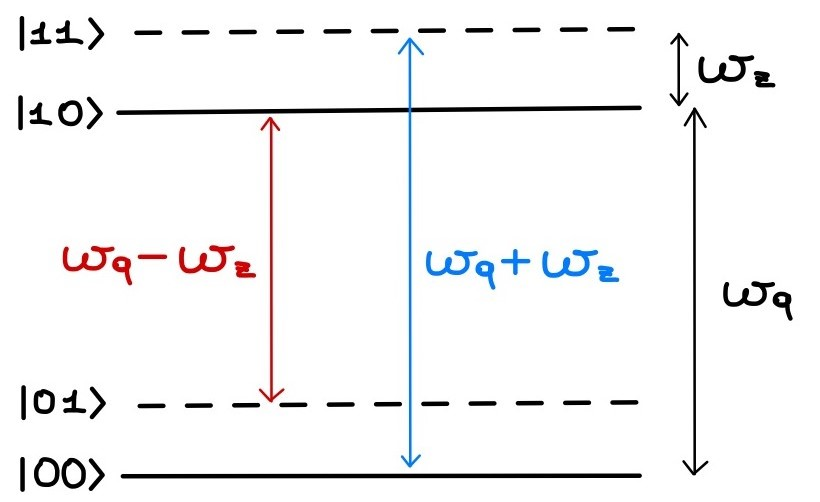
\includegraphics[scale=.45,keepaspectratio]{images/levels_ion_trap1}} \\
	\subfloat[][\label{subfig:levels_ion_trap2} ]{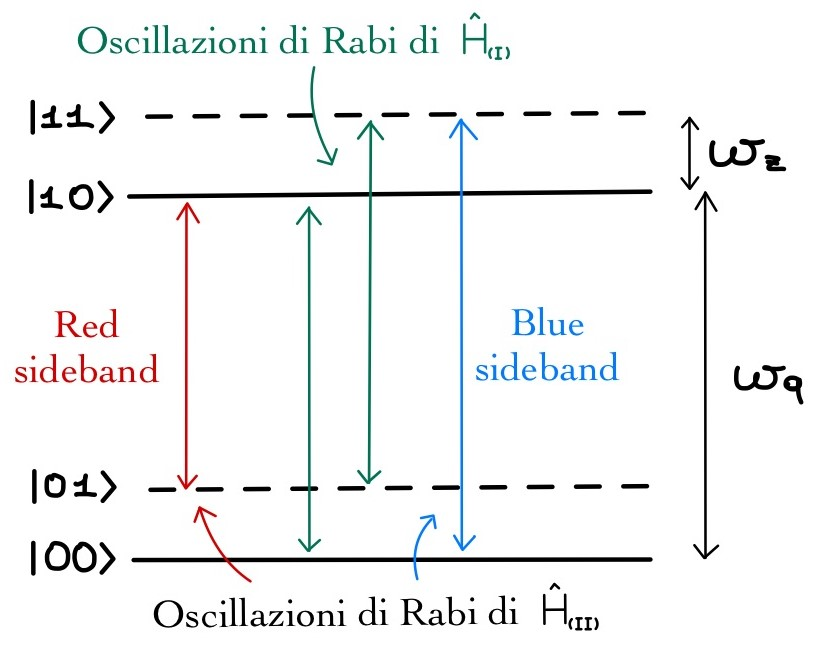
\includegraphics[scale=.45,keepaspectratio]{images/levels_ion_trap2}}
	\caption{(\ref{subfig:levels_ion_trap1}) Suddivisione dei livelli energetici degli ioni in un sistema a trappola ionica. Le frequenze $\omega_q - \omega_z$ e $\omega_q + \omega_z$ sono dette \textbf{red sideband} e \textbf{blue sideband} rispettivamente.  (\ref{subfig:levels_ion_trap2}) Oscillazioni di Rabi prodotte dai termini delle hamiltoniane $\hat{H}_{(I)}$ e $\hat{H}_{(II)}$. Notare che per la red sideband contribuiscono gli operatori $\hat{\sigma}_- \hat{a}$ ($\ket{01} \to \ket{10}$) e $\hat{\sigma}_+ \hat{a}^\dag$ ($\ket{10} \to \ket{01}$); mentre per la blue sideband contribuiscono $\hat{\sigma}_+ \hat{a}$ ($\ket{11} \to \ket{00}$) e $\hat{\sigma}_- \hat{a}^\dag$ ($\ket{00} \to \ket{11}$).}
    \label{fig:levels_ion_trap}
\end{figure}

\noindent Ci sono molti termini che possono contribuire a seconda della frequenza del laser. L'idea nei sistemi a trappola ionica è quella di utilizzare una radiazione che possa accomodare 4 differenti frequenze. Innanzitutto etichettiamo gli stati del sistema con la notazione $\ket{nm}$, dove $n$ è il livello energetico del qubit e $m$ il modo di oscillazione vibrazionale (fonone). Tenendo conto della Figura \ref{subfig:levels_ion_trap1} vorremmo utilizzare le 4 frequenze $\pm \omega_q \pm \omega_z$ e $\pm \omega_q$ (quest'ultimo permette le oscillazioni $\ket{0m} \leftrightarrow \ket{1m}$).

\noindent Scriviamo i termini che "sopravvivono" dalla RWA nelle due hamiltoniane $\hat{H}_{(I)}$ e $\hat{H}_{(II)}$:
\begin{align}
    \hat{H}_{(I)} &= \frac{\Omega}{2} \left( \hat{\sigma}_+ e^{i(\omega t - \phi)} + \hat{\sigma}_- e^{-i(\omega t - \phi)} \right) \label{H_I_Rabi} \\
    \hat{H}_{(II)} &= i \frac{\eta \Omega}{2} \left( -\hat{\sigma}_+ \hat{a}^\dag e^{i(\omega t - \phi)} + \hat{\sigma}_- \hat{a} e^{-i(\omega t - \phi)} \right) + \label{H_II_sideband} \\
    &\quad + i \frac{\eta \Omega}{2} \left( -\hat{\sigma}_+ \hat{a} e^{i(\omega t - \phi)} + \hat{\sigma}_- \hat{a}^\dag e^{-i(\omega t - \phi)} \right) \, , \notag
\end{align}
dove nella \eqref{H_I_Rabi} abbiamo assunto $\omega \sim \omega_q$ e nella \eqref{H_II_sideband} si ha $\omega \sim \omega_q - \omega_z$ nella prima riga e $\omega \sim \omega_q + \omega_z$ nella seconda (notare che $\omega$ in queste due righe è scelto appositamente per annullare le fasi derivanti dalla \eqref{RWA_ops_trans}). Come evidente dal disegno in Figura \ref{subfig:levels_ion_trap2}, $\hat{H}_{(I)}$ genera oscillazioni di Rabi tra $\ket{0 m} \leftrightarrow \ket{1m}$ se si utilizza un laser con frequenza $\omega \sim \omega_q$; similmente, le due righe di $\hat{H}_{(II)}$ hanno un comportamento analogo perché la blue sideband (seconda riga) genera oscillazioni di Rabi tra $\ket{11} \leftrightarrow \ket{00}$ e la red sideband (prima riga) produce oscillazioni di Rabi tra $\ket{01} \leftrightarrow \ket{10}$ (si faccia sempre riferimento alla Figura \ref{subfig:levels_ion_trap2} tenendo presente l'azione di $\hat{\sigma}_\pm$ sui livelli del qubit).  

\noindent La logica è quindi quella di utilizzare le oscillazioni di $\hat{H}_{(I)}$ per muovere il qubit lungo la sfera di Bloch (implementare gate agenti su singoli qubit) e le oscillazioni di $\hat{H}_{(II)}$ per codificare delle operazioni agenti contemporaneamente su due tipi differenti di qubit. Vediamo il più semplice esempio di costruzione di un tale gate.

\subsection{Cirac-Zoller gate}
Il \textbf{Cirac-Zoller gate} costituisce un esempio di realizzazione pratica di un \texttt{CNOT-gate}. Immaginiamo di considerare, in aggiunta ai livelli energetici nella Figura \ref{fig:levels_ion_trap}, un livello extra, che chiamiamo $\ket{2m}$, del sistema atomico: 
\begin{center}
    \mbox{
        $
        \begin{matrix}
        &\Qcircuit @C=2em @R=1.3em {
            \lstick{\ket{11}} & \qw & \qw & \qw \\
            \lstick{\ket{10}} & \qw & \qw & \qw
        }
        \\ \\ \\
        &\Qcircuit @C=2em @R=1.3em {
            \lstick{\ket{01}} & \qw & \qw & \qw \\
            \lstick{\ket{00}} & \qw & \qw & \qw
        }
        \end{matrix}
        $
    }
    \raisebox{0.6em}{\mbox{
        \Qcircuit @C=2em @R=1.3em {
            & \qw & \qw & \qw & \rstick{\ket{21}} \\
            & \qw & \qw & \qw & \rstick{\ket{20}}
        }
    }}
\end{center}
Chiamiamo $E_{10} - E_{20} = \omega_{\text{aux}}$ (aux per ausiliaria) e chiaramente poniamo come prima $E_{10} - E_{00} = \omega_q$. L'idea è quella di utilizzare un laser sintonizzato ad una frequenza $\omega = \omega_{\text{aux}} + \omega_z$ per produrre transizioni tra gli stati $\ket{20} \leftrightarrow \ket{11}$. Le oscillazioni di Rabi così prodotte, regolando opportunamente l'ampiezza, la fase e la frequenza del laser, possono essere parametrizzate come al solito
dall'operatore in \eqref{formula_for_Rabi}
\begin{equation*}
    R_{\vec{n}}(\gamma) = e^{-\frac{i}{2} \gamma (\vec{\sigma} \cdot \vec{n})} = \mathbb{I} \cos \! \left( \frac{\gamma}{2} \right) - i (\vec{\sigma} \cdot \vec{n}) \sin \! \left( \frac{\gamma}{2} \right) \, ;
\end{equation*}
se scegliamo di ruotare con angolo $2 \pi$ attorno ad $x$ allora 
\begin{equation*}
    R_x(2 \pi) = e^{-\frac{i}{2} 2 \pi \sigma_x} = \mathbb{I} \cos \pi - i \sin \pi \sigma_x = -\mathbb{I} \, ,
\end{equation*}
quindi una rotazione spaziale di 360° agisce in maniera non banale sui fermioni! (Si noti che questo è vero per qualsiasi direzione $\vec{n}$). Quindi se si scelgono dei laser opportuni che implementano trasformazioni $R_x(2\pi)$ e si aspetta del tempo a sufficienza, allora possiamo realizzare questa operazione sugli stati precedenti: $\ket{11} \to - \ket{11}$ e $\ket{20} \to -\ket{20}$. Se ci dimentichiamo dello stato ausiliario $\ket{20}$ (l'informazione è codificata negli stati $\ket{nm}$), allora l'effetto netto sul sistema non è altro che un \texttt{CZ-gate}
\begin{equation*}
    \begin{pmatrix}
        1 & & & \\ & 1 & & \\ & & 1 & \\ & & & -1
    \end{pmatrix}
    \begin{pmatrix}
        \ket{00} \\ \ket{01} \\ \ket{10} \\ \ket{11}
    \end{pmatrix}
    =
    \begin{cases}
        \ket{00} \to \ket{00} \\
        \ket{01} \to \ket{01} \\
        \ket{10} \to \ket{10} \\
        \ket{11} \to -\ket{11}
    \end{cases}
    \! \! = \; 
    \raisebox{1.4em}{\mbox{
        \Qcircuit @C=1em @R=1.2em {
            & \qw & \ctrl{1} & \qw & \qw \\
            & \qw & \gate{Z} & \qw & \qw
        }
    }}
\end{equation*}
perché l'operatore $Z$ viene applicato sul secondo qubit solamente quando il primo si trova in $\ket{1}$. Come già anticipato al termine della Sezione \ref{sec:int_qubit_CQED}, è molto semplice passare da un \texttt{CZ-gate} ad un \texttt{CNOT-gate}:
\begin{center}
    \mbox{
        \Qcircuit @C=1em @R=1.2em {
            & \qw & \ctrl{1} & \qw & \qw & \\
            & \qw & \targ & \qw & \qw &
        }
    }
    \raisebox{-1em}{= \;}
    \mbox{
        \Qcircuit @C=1em @R=1em {
            & \qw & \ctrl{1} & \qw & \qw & \\
            & \gate{H} & \gate{Z} & \gate{H} & \qw &
        }
    }
\end{center}
In generale è abbastanza semplice realizzare un \texttt{CZ-gate} sui qubit, ma è invece meno banale realizzare questa operazione sugli stati costruiti con i modi vibrazionali. Nonostante ciò, si può ovviare a questo problema ricordando che questo gate ha la proprietà
\begin{center}
    \mbox{
        \Qcircuit @C=1em @R=1.2em {
            & \qw & \ctrl{1} & \qw & \qw \\
            & \qw & \gate{Z} & \qw & \qw
        }
    }
    \raisebox{-1em}{\; = \;}
    \mbox{
        \Qcircuit @C=1em @R=1.2em {
            & \qw & \gate{Z} & \qw & \qw \\
            & \qw & \ctrl{-1} & \qw & \qw
        }
    }
\end{center}
perché il risultato è analogo a quello sopra anche se $Z$ agisce sul primo qubit quando il secondo è in $\ket{1}$: non importa dove è posto $Z$ perché si può equivalentemente applicare questo gate sul qubit (più semplice) o sui modi vibrazionali!

\noindent Questi risultati relativi alla realizzazione di operazioni su un insieme di due qubit furono un grande traguardo negli anni '90, tuttavia al giorno d'oggi si vorrebbe costruire un QC con $\sim 100$ qubit, quindi sarebbe veramente poco pratico creare un sistema entangled tra ioni e modi vibrazionali. Dato che nella trappole ioniche si allinea facilmente un array di qubit in cui essi sono creati separatamente, si vorrebbe codificare l'informazione solamente nei qubit realizzati dagli ioni e non in quelli ottenuti dai modi vibrazionali. Questo scopo può essere raggiunto sfruttando i modi vibrazionali come \textbf{bus}, ossia modi ausiliari, che muovono l'informazione da ione a ione.

\noindent Immaginiamo un generico array di qubit: vorremmo poter indirizzare operazioni a due qubit su due qubit ben precisi dell'array utilizzando in qualche modo i modi vibrazionali come step intermedio. Ciò può essere fatto per mezzo dei fononi e utilizzando il cosiddetto \texttt{SWAP-gate}, ossia un gate che scambia informazioni da un qubit ai modi vibrazionali e successivamente da questi ultimi ad un altro qubit. 

\noindent Immaginiamo ad esempio di voler scambiare gli stati  $\ket{01} \leftrightarrow \ket{10}$: questo può essere fatto per mezzo della matrice
\begin{equation*}
    \begin{pmatrix}
        1 & & & \\ & 0 & 1 & \\ & -1 & 0 & \\ & & & 1
    \end{pmatrix}
    \begin{pmatrix}
        \ket{00} \\ \ket{01} \\ \ket{10} \\ \ket{11}
    \end{pmatrix}
    = 
    \begin{pmatrix}
        \ket{00} \\ \ket{10} \\ \ket{01} \\ \ket{11}
    \end{pmatrix} \, ,
\end{equation*}
ma il blocco interno non è altro che una rotazione di Rabi di angolo $\pi$ lungo $y$:
\begin{equation*}
    \begin{pmatrix}
        0 & 1 \\ -1 & 0
    \end{pmatrix}
    = i \sigma_2 =
    \cos \! \left( \frac{\pi}{2} \right) + i \sin \! \left( \frac{\pi}{2} \right) \sigma_2 = e^{\frac{i}{2} \pi \sigma_2} = R_y(-\pi) \, .
\end{equation*}
Riusciamo a codificare in qualche modo un'oscillazione di Rabi che operi con $R_y(-\pi)$ su $\ket{01}$ e $\ket{10}$? La risposta è affermativa perché possiamo utilizzare una delle frequenze di sideband dell'hamiltoniana in  \eqref{H_II_sideband}: ad esempio possiamo impiegare la red sideband (prima riga) per implementare tutti i possibili operatori $R_{\vec{n}}(\gamma)$ agenti sul sottospazio $\{ \ket{01}, \ket{10} \}$. Come funziona questo \texttt{SWAP-gate}? Immaginiamo di partire in uno stato dato dal prodotto tensoriale di un modo senza fononi e un qubit arbitrario dell'array di ioni: 
\begin{equation*}
    \left( a \ket{0} + b \ket{1} \right) \otimes \ket{0} = a \ket{00} + b \ket{10} \overset{\texttt{SWAP}}{\longrightarrow} a \ket{00} + b \ket{01} = \ket{0} \otimes \left( a \ket{0} + b \ket{1} \right) \, ,
\end{equation*}
è quindi possibile scambiare informazioni che erano codificate nel qubit con lo stato del modo vibrazionale. Successivamente si agisce con un altro \texttt{SWAP-gate} e si sceglie un altro ione nel quale trasferire l'informazione acquisita. 

\noindent Più esplicitamente, etichettiamo gli ioni dell'array con $j,k = 1, 2, 3, 4, \ldots$; ora mostriamo che è possibile costruire un gate $\texttt{CZ}_{(i)}$ per ogni ione (gate che coinvolge il sistema combinato fononi-ioni) e poi agire con un \texttt{SWAP-gate} su ciascun ione per trasferire l'informazione e utilizzare quindi i modi vibrazionali come \textbf{bus}. 

\begin{esempio}[\textbf{\texttt{CZ-gate} e \texttt{CNOT-gate} tra ioni}]
    Supponiamo di voler realizzare un \texttt{CZ-gate} tra due ioni generici $j$ e $k$, dove quest'ultimo agisce come control-qubit sul primo. Possiamo agire con $\texttt{SWAP}_k$ per muovere l'informazione da $k$ ai fononi, applicare $\texttt{CZ}_j$ tra i fononi e lo ione $j$ e infine ritornare allo ione $k$ con $\texttt{SWAP}^{-1}_k$: in ordine significa applicare le operazioni
    \begin{equation*}
        \texttt{SWAP}^{-1}_k \, \texttt{CZ}_j \, \texttt{SWAP}_k \, .
    \end{equation*}
    
    \noindent La stessa procedura può essere applicata per l'implementazione di un \texttt{CNOT-gate} con l'unica differenza che è necessario aggiungere due \texttt{H-gate} prima e dopo: 
    \begin{equation*}
        H_k \texttt{SWAP}^{-1}_k \, \texttt{CZ}_j \, \texttt{SWAP}_k H_k \, .
    \end{equation*}
\end{esempio}

\noindent Storicamente questa procedura per costruire un 2-qubit gate fu importante perché fu il primo esempio di implementazione di operazioni agenti su due qubit contemporaneamente in una trappola ionica. Oggigiorno è considerato un esempio per lo più di importanza storica e non pratica, perché per far sì che lo scambio dell'informazione con lo \texttt{SWAP-gate} avvenga è necessario partire con un sistema senza fononi, cosa che è raggiunta senza non poche difficoltà raffreddandolo con dei laser.   

\noindent Sarebbe decisamente più conveniente poter lavorare con dei gate che funzionino con un numero arbitrario di fononi. Questo è il caso del seguente esempio.

\subsection{M\o lmer-S\o rensen gate}
Non entriamo nel dettaglio della discussione di questo gate, tuttavia ci limitiamo a notare che si tratta di un'altra situazione in cui si necessita risolvere un ingegnoso esercizio in QM. L'idea peculiare è quella di considerare un laser bicromatico (irradia con 2 frequenze differenti) che possa indirizzare 2 o più ioni simultaneamente, i quali possono avere stati intermedi con $n-1$, $n$ e $n+1$ fononi. Denotando come al solito con $\ket{e}, \, \ket{g}$ gli stati del qubit e con $\ket{n}$ i modi vibrazionali dei fononi, facciamo riferimento alla Figura \ref{subfig:molmer_sorensen1}. Supponiamo che esistano alcuni stati intermedi tra $\ket{ggn}$ e $\ket{een}$: è possibile utilizzare un laser con una frequenza leggermente desintonizzata di un fattore $\delta$ per mandare lo stato $\ket{ggn}$ alla sovrapposizione di stati immediatamente prima di $\ket{eg \, n+1}$; successivamente si sceglie la seconda frequenza del laser bicromatico in maniera tale che permetta poi la transizione fino a $\ket{een}$ (vedi frecce rosse). Ovviamente la stessa cosa può essere fatta invertendo le frequenze del laser (vedi frecce blu). Esplicitamente le due frequenze del laser bicromatico sono $\omega = \omega_q \pm (\omega_z - \delta)$. 

\begin{figure}[!h]
	\centering	
	\subfloat[][\label{subfig:molmer_sorensen1} ]{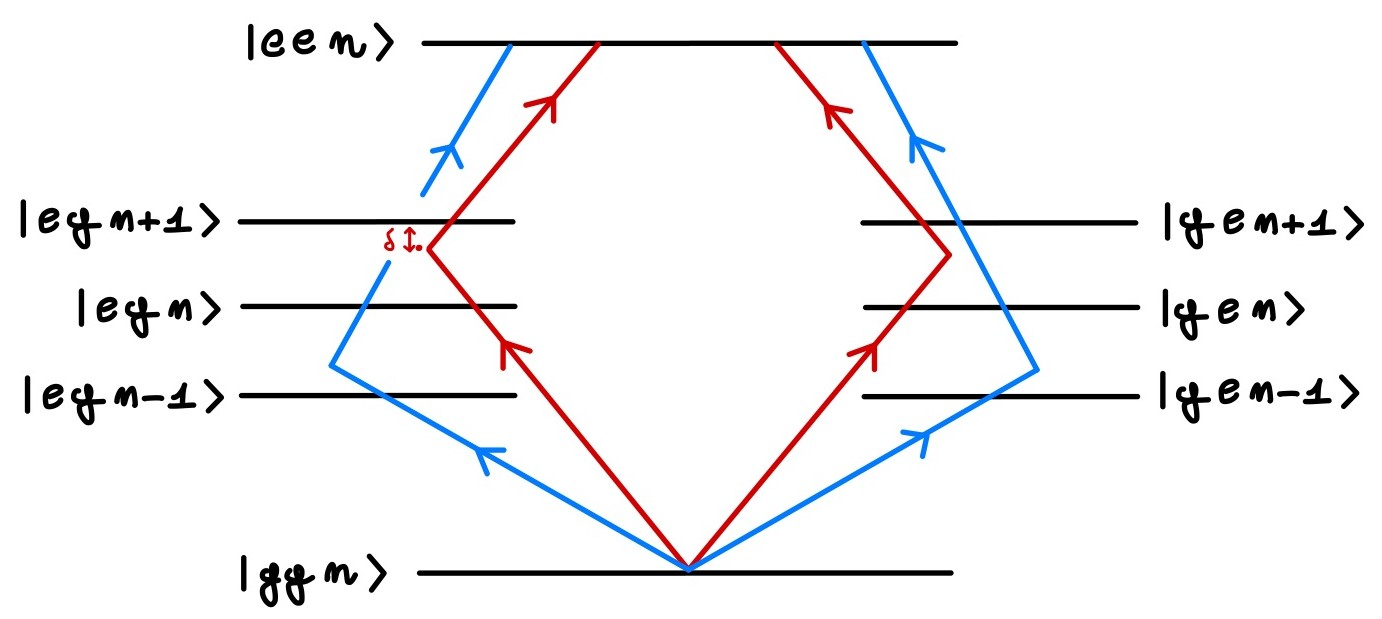
\includegraphics[scale=.31,keepaspectratio]{images/molmer_sorensen1}} \\
	\subfloat[][\label{subfig:molmer_sorensen2} ]{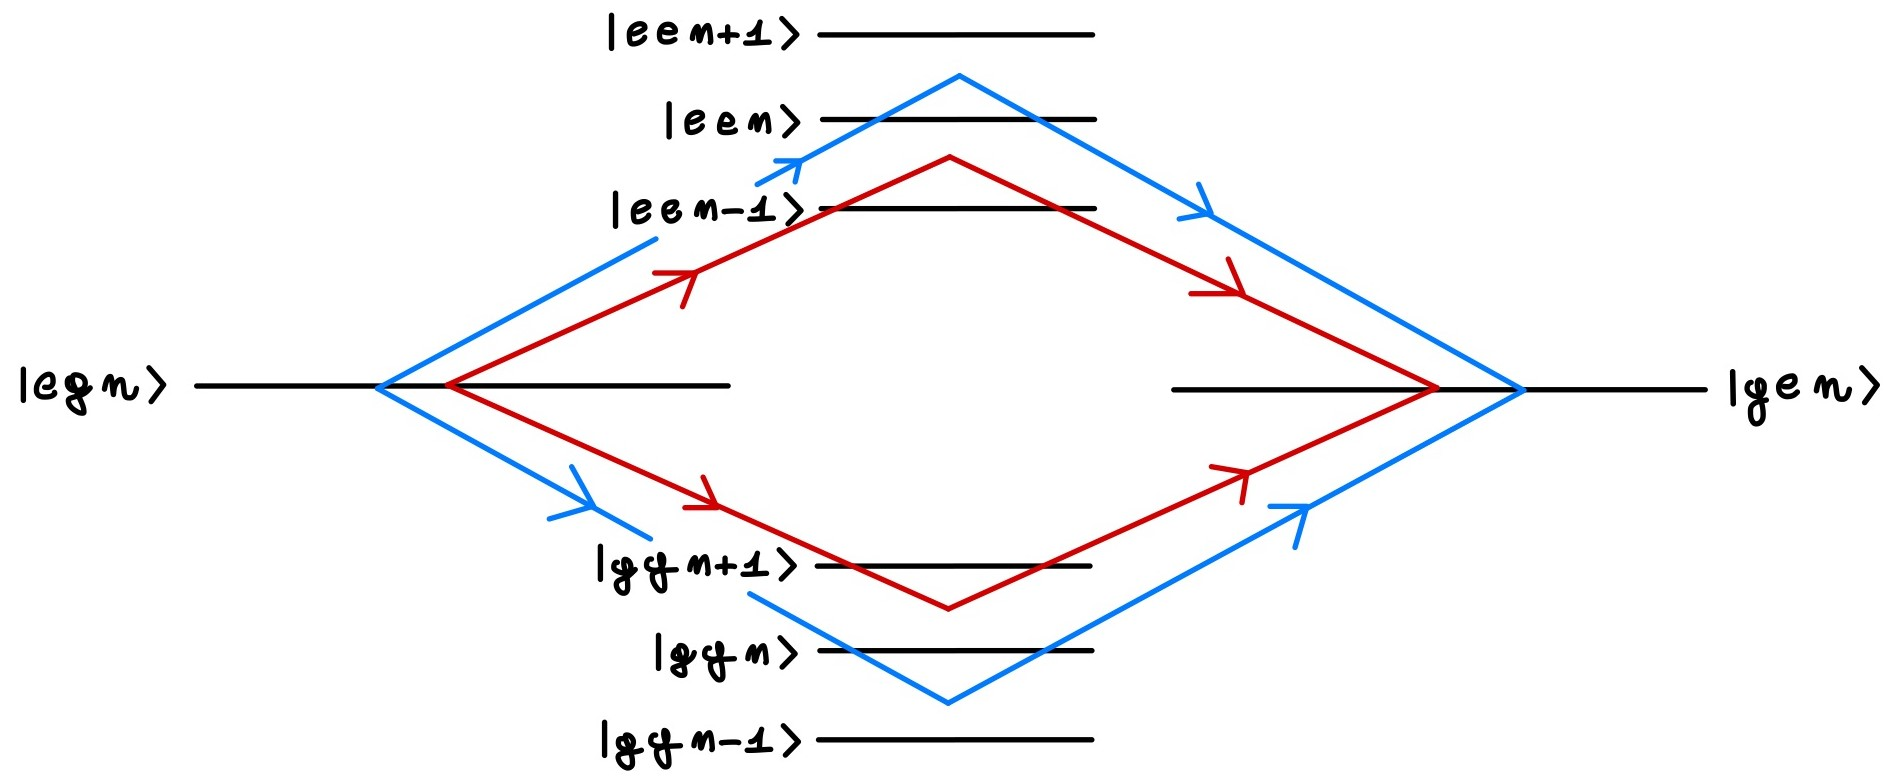
\includegraphics[scale=.31,keepaspectratio]{images/molmer_sorensen2}}
	\caption{(\ref{subfig:molmer_sorensen1}) Oscillazioni di Rabi che connettono gli stati $\ket{ggn} \leftrightarrow \ket{een}$ nel M\o lmer-S\o rensen gate. (\ref{subfig:molmer_sorensen2}) Caso analogo al precedente in cui sono connessi gli stati $\ket{egn} \leftrightarrow \ket{gen}$.}
    \label{fig:molmer_sorensen}
\end{figure}

\noindent Come mostrato in Figura \ref{subfig:molmer_sorensen2}, lo stesso setup può essere utilizzato per connettere gli stati $\ket{egn} \leftrightarrow \ket{gen}$: è quindi possibile, in generale, creare oscillazioni di Rabi tra gli stati $\ket{ggn} \leftrightarrow \ket{een}$ e $\ket{egn} \leftrightarrow \ket{gen}$. 

\noindent Questa tipologia di trasformazioni sono al secondo ordine in teoria delle perturbazioni: gli stati intermedi non sono mai realmente popolati perché per poter effettuare operazioni sui qubit per mezzo delle oscillazioni di Rabi è necessario lavorare alla risonanza. In generale questo non è del tutto ovvio, tuttavia la cosa molto ingegnosa sta nel fatto che le oscillazioni di Rabi risultanti sono del tutto indipendenti dal numero $n$ di fononi! Dunque non è più necessario raffreddare il sistema. 

\noindent Per mostrarlo rigorosamente è necessario svolgere un conto completo in teoria delle perturbazioni dipendenti dal tempo. Intuitivamente si può notare che, dato che $\hat{H}_{\text{int}} \sim (\hat{a} + \hat{a}^\dag)$, allora negli stati dei modi vibrazionali si possono avere solamente un fonone in più o un fonone in meno rispetto allo stato di partenza, quindi $\ket{m} = \ket{n+1}$ oppure $\ket{m} = \ket{n-1}$; ciò è dato dal fatto che solamente gli elementi di matrice di questi stati intermedi sono diversi da zero, ossia $\mel{n}{\hat{a}}{n+1} = \sqrt{n+1}$ e $\mel{n}{a^\dag}{n-1} = \sqrt{n}$. Per questo motivo, un calcolo in teoria delle perturbazioni per campo debole produce  un'ampiezza di Rabi  indipendente da $n$:
\begin{equation*}
    \begin{large}\substack{\text{Ampiezza} \\
    \text{di Rabi}}\end{large} \sim \sum_m \frac{\mel{een}{\hat{H}_{\text{int}}}{m} \mel{m}{\hat{H}_{\text{int}}}{ggn}}{E_m - E_{ggn} - \omega} \sim \frac{(n+1)}{\delta} + \frac{n}{-\delta} \sim \frac{1}{\delta} \, .
\end{equation*}
Un conto pi\`u completo  in approssimazione RWA consente di calcolare esattamente l'operatore di evoluzione temporale che ha la forma
\begin{equation*}
    \hat{U}(t) \sim e^{\alpha(t) \hat{a} + \alpha^\ast(t) \hat{a}^\dag + i S^2_y \beta(t)} \, , \quad \text{dove} \quad S_y = \sigma_1^{(1)} + \sigma_y^{(2)} \, ,
\end{equation*}
dove $\alpha(t)$ e $\beta(t)$ sono due funzioni del tempo calcolabili. Scegliendo i valori del tempo che risolvono l'equazione $\alpha(t) = 0$, l'operatore di evoluzione temporale diventa indipendente dagli oscillatori associati ai fononi e produce un gate universale che realizza l'entanglement tra due qubit.
    %%%%%%%%%%%%%%
% LECTURE 20 %
%%%%%%%%%%%%%%
\vspace{1cm}

\noindent\lecture{20}{17/12/2021}
\section{Sistemi superconduttivi}
Dopo aver studiato e analizzato i sistemi a trappola ionica, diamo uno sguardo, in maniera del tutto generale, a un altro modo, molto diffuso e utilizzato, di andare a realizzare sistemi a due livelli: i \textbf{sistemi superconduttivi}. Spesso vengono anche definiti come \textbf{circuiti QED} (\textbf{cQED}) in analogia proprio con le cavità QED (CQED). Negli esempi analizzati nel caso della CQED si sfruttava il fatto che un semplice modello possa essere utilizzato per descrivere l'interazione di un atomo con una cavità ottica oppure anche per spiegare l'accoppiamento di un qubit con un risonatore a microonde: questo modello include il numero di fotoni nella cavità/risonatore, lo stato dell'atomo/qubit e l'interazione del dipolo elettrico tra l'atomo/qubit e la cavità/risonatore.

\noindent Invece, come suggerisce il nome, la fisica che sta dietro ai sistemi superconduttivi sfrutta il fenomeno della superconduttività. Per una trattazione completa sarebbe richiesto un corso intero, per cui, nel nostro studio, ci limitiamo a riportare i risultati generali che serviranno a descrivere questo tipo di sistemi.

\subsection{Cenni di superconduttività}

L'idea alla base della realizzazione fisica dei qubit è abbastanza semplice, tuttavia la fisica che ci sta dietro è abbastanza complessa perché coinvolge il concetto della \textbf{superconduttività}. Prima di vedere come si realizza la costruzione dei qubit e dei gate, facciamo alcuni cenni su questo importante argomento. 

\noindent Che cos'è la superconduttività? In corrispondenza di temperature sufficientemente basse, elementi metallici ed alcuni semiconduttori vanno incontro ad una transizione di fase. Al di sotto di una particolare temperatura, detta temperatura critica $T_C$, essi acquistano notevoli proprietà fisiche; la loro resistività
diventa bruscamente nulla, perciò in questi materiali diventa possibile, in assenza di campi esterni, misurare correnti che non decadono nel tempo. L’assenza di effetti dissipativi nel meccanismo di conduzione, assieme ad altri fenomeni correlati, sono indicati sinteticamente con il termine \textbf{superconduttività}. Nel 1957 J. Bardeen, L. N. Cooper e J. R. Schrieffer, formularono la prima teoria microscopica della superconduttività (\textbf{teoria BCS}) utilizzando la meccanica quantistica, che valse loro il Nobel nel 1972. Tale teoria è in grado di dare una spiegazione del fenomeno della superconduzione (capacità predittiva e base per le applicazioni). 

\noindent Il fenomeno della superconduttività consiste nella creazione, per mezzo dello scambio di fononi nel metallo e a temperatura sufficientemente bassa, di stati legati costituiti da coppie di elettroni $(e^-,e^-)$, chiamate \textbf{coppie di Cooper}. Questi oggetti sono ovviamente bosoni e costituiscono un particolare condensato di Bose-Einstein.

\noindent In questa configurazione, mentre i fermioni, a causa del principio di esclusione di Pauli, sono disposti in maniera tale da non avere lo stesso set di numeri quantici, i bosoni, a basse temperature, sono tutti situati nello stato fondamentale. In un metallo regolare se gli elettroni vengono messi in moto, tipicamente, per via della presenza di impurezze o reticoli di cristallo con cui gli elettroni fanno scattering, vi è una resistenza. La stessa situazione vale per i bosoni, ma vi è una interazione di scambio: è energicamente favorevole mettere i bosoni nello stesso stato (stesso set di numeri quantici), in particolare nello stato fondamentale perché per spostare uno di questi bosoni è richiesta una grande quantità di energia. La corrente che si viene a originare è un flusso di bosoni, tutti con la stessa velocità e dato che è richiesta energia per rimuovere un bosone dallo stato in cui si trovano tutti gli altri, hanno tutti una bassa resistenza. Un esempio di spettro energetico a basse temperature di un materiale superconduttivo è dato dalla Figura \ref{fig:super-spectrum}.

\begin{figure}[!ht]
    \centering
    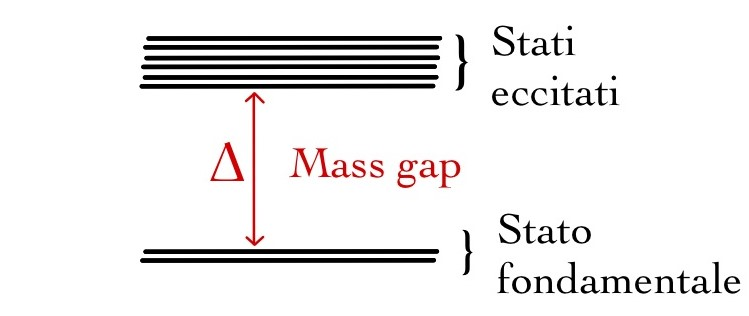
\includegraphics[scale=0.45]{images/super-spectrum.jpg}
    \caption{Spettro energetico di un materiale superconduttivo. La differenza tra lo stato fondamentale e gli stati eccitati è noto come \textbf{mass gap} $\Delta$.}
    \label{fig:super-spectrum}
\end{figure}


\subsection{cQED}

L'idea è quella di realizzare dei qubit con dei piccoli circuiti superconduttivi (non si tratta più di un sistema atomico o di spin). Un tale sistema sembrerebbe a prima vista macroscopico, tuttavia, come vedremo, grazie alla presenza del fenomeno della superconduttività è davvero quantistico. 

\begin{figure}[H]
    \centering
    \begin{circuitikz}
        \draw
        (0,0)   to[C=$C$] ++ (0, 2) -- ++ ( 2,0) 
                to[L=$L$] ++ (0,-2) -- ++ (-2,0)
                (1,0)node[ground]{};
    \end{circuitikz}
    \caption{Circuito LC.}
    \label{fig:lc-circuit}
\end{figure}

\noindent Ancora una volta si utilizza un oscillatore armonico: affinché si possa utilizzare come un sistema a due livelli è necessario introdurre dell'anarmonicità nei livelli energetici così da poter distinguere lo stato fondamentale dal primo eccitato senza preoccuparsi degli altri livelli. Il nostro punto di partenza è un semplice \textbf{circuito LC}, come mostrato in Figura \ref{fig:lc-circuit}.

\noindent Vediamo il motivo per cui un tale circuito presenta un comportamento oscillatorio. Innanzitutto, ricordiamo che ciascun elemento mette in relazione la carica o la corrente con il potenziale; in particolare le relazioni costitutive della capacità e dell'induttanza risultano:
\begin{align*}
    &\text{Capacità:} &Q & =CV\, , \\
    &\text{Induttanza:} &V &= L\dv{I}{t}\, .
\end{align*}
Per svolgere questo tipo di trattazione può tornare utile riscrivere la corrente come $I=\dv{Q}{t}$ e introdurre il \textit{flusso} definito come
\begin{equation*}
    \Phi(t)=\int_{-\infty}^{t} \dd{t'} V(t') \, ;
\end{equation*}
a questo punto, la relazione sull'induttanza può, ad esempio, essere riscritta in termini di flusso integrando entrambi i membri 
\begin{equation*}
    \Phi = LI \, .
\end{equation*}
Note le relazioni tra carica/corrente e potenziale, possiamo andare a valutare le energie associate a ciascun elemento del circuito. A partire da
\begin{equation}\label{eq:general-energy}
    E(t)=\int_{-\infty}^{t} \dd{t'} V(t')I(t') \quad (\text{da } \delta E = V \delta Q) \, ,
\end{equation}
assumendo che tutte le quantità in gioco si annullino a $t=-\infty$, ricaviamo
\begin{align*}
    &\text{Capacità:} &E&=\int_{-\infty}^{t} \dd{t'} VC\derivative{V}{t'}=\frac C 2 V^2 = \frac{Q^2}{2C} \, , \\
    &\text{Induttanza:} &E&=\int_{-\infty}^{t} \dd{t'} L\derivative{I}{t'}I=\frac L 2 I^2 \equiv \frac{\Phi^2}{2L}\, .
\end{align*}
In una trattazione classica possiamo interpretare il termine relativo alla capacità come un'\textbf{energia cinetica} mentre quello relativo all'induttanza come \textbf{energia potenziale}. In questo contesto possiamo andare a scrivere la lagrangiana classica del sistema nel seguente modo
\begin{align*}
    \mathcal{L}&= E_k - E_p = \frac{Q^2}{2C}-\frac{\Phi^2}{2L} = \frac{C}{2}V^2-\frac{\Phi^2}{2L} = \frac{C}{2}\dot{\Phi}^2-\frac{\Phi^2}{2L} \, ,
\end{align*}
dove abbiamo inserito il fatto che $V = \dv{\Phi}{t}$. Applicando le equazioni di Eulero-Lagrange
\begin{equation*}
    \dv{t} \left(\pdv{\mathcal{L}}{\dot{\Phi}}\right)-\pdv{\mathcal{L}}{\Phi}=0 \, ,
\end{equation*}
si ottiene l'equazione del moto
\begin{equation*}
    C\ddot{\Phi}+\frac{\Phi}{L}=0 \, ,
\end{equation*}
che possiamo riscrivere sotto forma di equazione del moto di un oscillatore armonico nel seguente modo
\begin{equation*}
    \ddot{\Phi}+\omega^2\Phi = 0 \, , \quad \text{con} \quad \omega=\frac{1}{\sqrt{LC}} \, .
\end{equation*}
Per passare ad una descrizione quantistica del sistema dobbiamo riscrivere la fisica nel formalismo hamiltoniano. Calcoliamo il \textit{momento coniugato}
\begin{equation*}
    \Pi = \fdv{\mathcal{L}}{\dot{\Phi}} = C\dot{\Phi} = CV = Q\, ,
\end{equation*}
cosicché possiamo calcolarci la \textit{trasformata di Legendre} della lagrangiana precedente
\begin{equation}\label{eq:ham-LC}
        H = \Pi\dot{\Phi} - \mathcal{L} = Q\frac QC - \left(\frac{Q^2}{2C}-\frac{\Phi^2}{2L}\right) = \frac{Q^2}{2C} + \frac{\Phi^2}{2L} \, ;
\end{equation}
è evidente che l'hamiltoniana corrisponde proprio alla somma dell'energia cinetica e dell'energia potenziale.

\noindent Supponiamo ora di considerare il medesimo sistema, ma di volerne dare una descrizione quantistica. In Tabella \ref{tab:oa-lc} sono riportate le relative identificazioni con il nuovo sistema quantistico.
\begin{table}[H]
	\centering
    \begin{tabular}{c|c}
        \toprule
        Oscillatore armonico & Circuito LC \\
        \midrule
        $H=\frac{\hat{p}^2}{2m}+\frac{m}{2}\omega^2\hat{x}$ & $H=\frac{Q^2}{2C}+\frac C2 \omega^2\Phi^2$ \\
        \midrule
        $\hat{x}$ & $\Phi$ \\
        \hline
        $\hat{p}$ & $Q$ \\
        \hline
        $m$ & $C$ \\
        \bottomrule
    \end{tabular}\\
    \caption{Identificazioni tra quantità fisiche e operatori dell'oscillatore armonico quantistico e le grandezze fisiche di un circuito LC. Si ricordi che per il circuito LC la frequenza è $\omega = \frac{1}{\sqrt{LC}}$.}
    \label{tab:oa-lc}
\end{table}
\noindent Possiamo quindi mappare un circuito LC con un oscillatore armonico e imporre la quantizzazione canonica per quantizzare un tale sistema. Possiamo promuovere $(\Phi, Q) \to (\hat{\Phi}, \hat{Q})$ ad operatori e scriverli in funzioni degli operatori di creazione e distruzione
\begin{equation}\label{Phi_Q_oscill}
    \hat \Phi = \sqrt{\frac{\hbar}{2C\omega}}\left(\hat a + \hat a^\dagger\right) \, , \qquad \hat Q = \frac{\sqrt{2C \omega \hbar}}{2i}\left(\hat a - \hat a^\dagger\right) \, ;
\end{equation}
in questo modo imponiamo le seguenti regole di commutazione
\begin{equation*}
    \comm{\hat \Phi}{\hat Q}=i\hbar \, , \quad \Leftrightarrow \quad \comm{\hat a}{\hat a^\dagger}=1 \, .
\end{equation*}
È dunque evidente che la procedura di quantizzazione è immediata, tuttavia è abbastanza insolito pensare di svolgere una trattazione quantistica di un sistema macroscopico. 
\noindent Se supponiamo invece di considerare un sistema superconduttivo, possiamo utilizzare alcuni risultati della teoria BCS per riscrivere l'hamiltoniana della relazione \eqref{eq:ham-LC} nel seguente modo
\begin{equation}\label{eq:ham-oa-cQED}
    \hat H = 4E_C\hat n^2 + \frac{E_L}{2}\hat \phi^2 \, , \quad \text{con} \quad \hbar\omega=\sqrt{8E_LE_C} \, ,
\end{equation}
dove
\begin{itemize}
    \item $\hat n = \frac{Q}{2e}$ è l'operatore che indica il numero di coppie di Cooper;
    \item $\hat \phi = \frac{2\pi}{\Phi_0}\Phi$ è l'operatore del flusso ridotto ($\Phi_0=\frac{h}{2e}$ è il \textit{quanto di flusso});
    \item $E_C=\frac{e^2}{2C}$ è l'energia necessaria per aggiungere un elettrone extra alla capacità del circuito;
    \item $E_L=\left(\frac{\Phi_0}{2\pi}\right)^2\frac 1 L$ è l'energia associata all'induttanza.
\end{itemize}
L'altro fatto fondamentale, accanto all'utilizzo di materiali superconduttivi, che rende il sistema adatto ad una descrizione quantistica è che in realtà non andiamo a utilizzare un circuito LC generico (il quale presenta infiniti livelli energetici equidistanti), ma uno in cui si introduce una cosiddetta \textbf{giunzione Josephson} (Figura \ref{subfig:JJ-circuit}). Quest'ultima produce il cosiddetto \textbf{effetto Josephson} (Figura \ref{subfig:J-effect}),  introducendo quindi dell'anarmonicità. 

\begin{figure}[!ht]
	\centering	
	\subfloat[][\label{subfig:JJ-circuit}]{
	    \begin{circuitikz}
        \draw
        (0,0)   to[C=$C$] ++ (0, 2) -- ++ ( 2,0) 
                to[josephson=$L$] ++ (0,-2) -- ++ (-2,0)
                (1,0)node[ground]{};
    \end{circuitikz}
	} \qquad
	\subfloat[][\label{subfig:J-effect}]{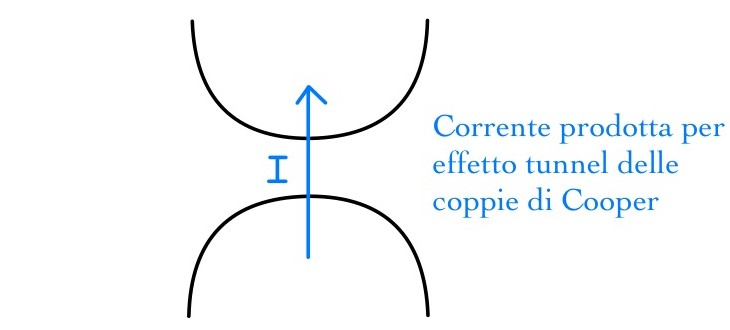
\includegraphics[scale=.4,keepaspectratio]{images/J-effect.jpg}}
	\caption{(\ref{subfig:JJ-circuit}) Circuito LC con giunzione Josephson (la giunzione è caratterizzata da una propria capacità $C_J$ e induttanza $L_J$). D'ora in avanti indicheremo nei circuiti una giunzione Josephson con la notazione di questo circuito. (\ref{subfig:J-effect}) Effetto tunnel della coppia di Cooper tra due elettrodi metallici superconduttivi sufficientemente vicini e separati da una sottile barriera di ossido.}
\end{figure}
\noindent L'effetto Josephson può essere riassunto nei seguenti due risultati:
\begin{enumerate}
    \item La corrente prodotta per effetto tunnel delle coppie di Cooper segue la \textbf{prima legge di Josephson}
    \begin{equation}\label{1_Josephson_law}
        I = I_C \sin \phi \, ,
    \end{equation}
    dove $I_C$ è detta \textbf{corrente critica};
    
    \item Applicando una differenza di potenziale ai capi degli elettrodi scorrerà un'altra corrente, la quale segue la \textbf{seconda legge di Josephson}
    \begin{equation}\label{2_Josephson_law}
        V = \dv{\Phi}{t} = \frac{\hbar}{2 e} \dv{\phi}{t} \, .
    \end{equation}
\end{enumerate}
Se si costruisce un circuito LC inserendo questa giunzione è possibile ricalcolare l'energia potenziale associata al circuito sfruttando la relazione in \eqref{eq:general-energy} 
\begin{equation}\label{eq:E_Josephson}
    E=\int_{-\infty}^{t} \dd{t'} V(t')I(t')=\frac{\hbar}{2e}I_C\int_{-\infty}^{t} \dd{t'} \derivative{\phi}{t'}\sin\phi =-E_J\cos\phi \, ,
\end{equation}
dove abbiamo indicato l'\textbf{energia Josephson} con $E_J = \frac{\hbar I_C}{2e}$. In questo modo l'hamiltoniana di un sistema di questo tipo risulta in
\begin{equation}\label{eq:ham-jj}
    \hat H = 4E_C\hat n^2-E_J\cos\hat \phi \, ,
\end{equation}
che differisce dalla \eqref{eq:ham-oa-cQED} per la presenza di un potenziale periodico anarmonico. In Figura \ref{fig:jj-spectrum} si può osservare lo spettro energetico dell'hamiltoniana che descrive un circuito LC con giunzione Josephson. L'obiettivo è quello di utilizzare per la costruzione di un qubit i livelli energetici evidenziati in figura: il punto fondamentale è stato l'introduzione della giunzione Josephson, la quale non solo rende il sistema veramente quantistico, ma soprattutto introduce dell'anarmonicità nello spettro dell'oscillatore. 

\begin{figure}[!ht]
    \centering
    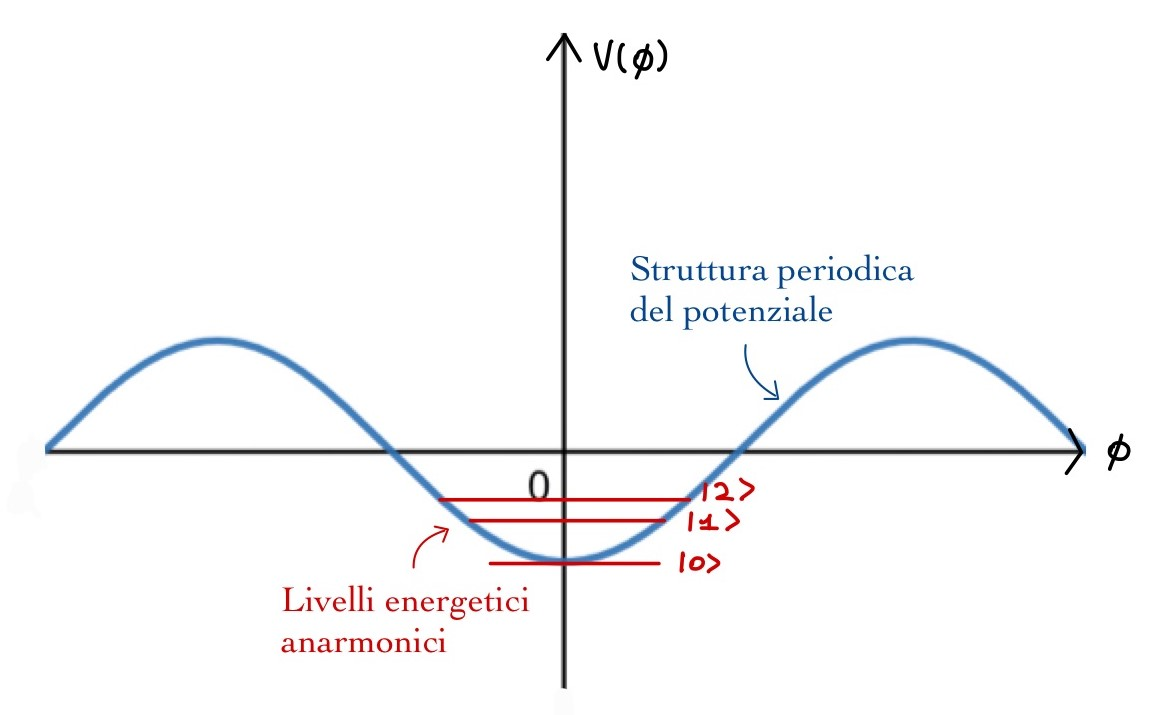
\includegraphics[scale=0.35]{images/jj-spectrum.jpg}
    \caption{Spettro energetico dell'hamiltoniana in \eqref{eq:ham-jj}. Per piccoli $\phi$ possiamo approssimare lo spettro come dei livelli energetici dell'oscillatore armonico più piccole correzioni anarmoniche.}
    \label{fig:jj-spectrum}
\end{figure}


\subsection{Interpretazione dell'effetto Josephson}
Per parlare in maniera del tutto completa ed esaustiva dell'effetto Josephson sarebbe necessaria una lezione completa, pertanto per approfondimenti e chiarimenti rimandiamo a corsi sulla superconduttività. 

\noindent L'idea che seguiamo è quella di procedere attraverso una trattazione schematica dell'effetto Josephson dovuta a Feynman. Il punto di partenza è la differenza nello spettro energetico che c'è tra un metallo normale, dove possiamo avere bande che sono riempite da un mare di elettroni (Figura \ref{subfig:metal-energy-spectrum}) e un superconduttore, in cui vi è una netta separazione tra lo stato fondamentale e gli stati eccitati (Figura \ref{subfig:superconductor-energy-spectrum}). 

\noindent Nel momento in cui andiamo a considerare una giunzione metallica come in basso in Figura \ref{subfig:metal-energy-spectrum}, costituita da due elettrodi ciascuno con il proprio mare di elettroni riempito fino all'energia di Fermi $\varepsilon_F$, e supponiamo che tra i due vi sia una differenza di potenziale $V$, allora possiamo osservare una corrente $I$ che scorre tra i due terminali dovuta al fatto che gli elettroni possano fare tunneling da un elettrodo a un altro. Questa corrente $I$ sarà proporzionale alla tensione applicata $V$ e il coefficiente di proporzionalità è dato dall'inverso della resistenza $R$ del sistema. Supponiamo invece di considerare due metalli superconduttivi, che indichiamo con (L) left e (R) right, ciascuno caratterizzato da un mass-gap $\Delta$: a basse temperature, dove la fisica della superconduttività è rilevante, quello che succede è che gli stati fondamentali di entrambi saranno occupati da un certo numero di coppie di Cooper $N_L$ e $N_R$; in tale situazione il tunneling è dovuto alle coppie di Cooper, da sinistra verso destra e viceversa.

\begin{figure}[!ht]
	\centering	
	\subfloat[][\label{subfig:metal-energy-spectrum}]{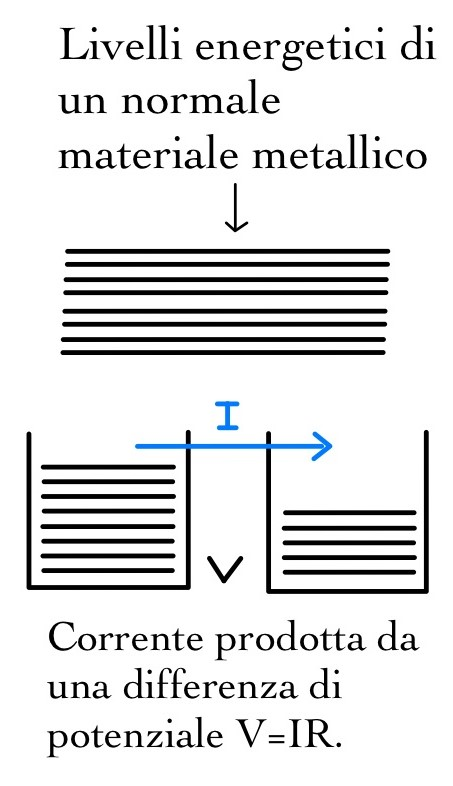
\includegraphics[scale=.3,keepaspectratio]{images/metal-energy-spectrum}} \qquad \qquad
	\subfloat[][\label{subfig:superconductor-energy-spectrum}]{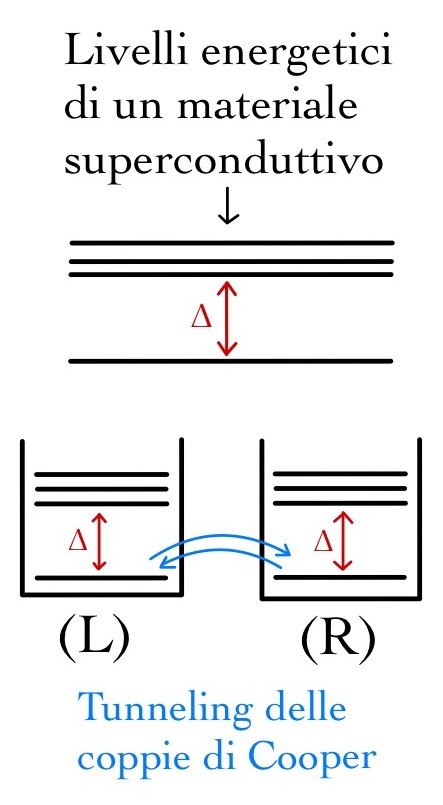
\includegraphics[scale=.3,keepaspectratio]{images/superconductor-energy-spectrum}} \qquad
	\caption{(\ref{subfig:metal-energy-spectrum}) Livelli energetici di un metallo caratterizzato da un mare di elettroni e sistema di due elettrodi in cui avviene il fenomeno del tunneling di elettroni da un elettrodo all'altro. (\ref{subfig:superconductor-energy-spectrum}) Livelli energetici di un metallo superconduttivo caratterizzato, a basse temperature, da uno stato fondamentale in cui si trovano tutte le coppie di Cooper e i livelli eccitati separati da un mass-gap $\Delta$ e sistema di due elettrodi superconduttivi in cui avviene il fenomeno del tunneling di coppie di Cooper da un elettrodo all'altro.}
\end{figure}

\noindent Dal punto di vista della QM, se la temperatura è sufficientemente bassa a tal punto da non considerare gli stati eccitati, ciò che conta è il numero quantico che identifica quanti bosoni sono nello stato fondamentale. Nel nostro caso, il sistema dei due elettrodi superconduttivi è descritto da due interi $N_L$ e $N_R$ (numero di coppie di Cooper nello stato fondamentale presenti rispettivamente nell'elettrodo di sinistra e nell'elettrodo di destra). Passare da un elettrodo all'altro significa quindi andare a incrementare e diminuire il numero di bosoni di entrambi gli elettrodi: ad esempio
\begin{equation*}
    \substack{\text{Tunneling di} \\ \text{un bosone da} \\ \text{(L) a (R)}}: \quad \ket{N_L, N_R} \longrightarrow \ket{N_L-1, N_R+1}
\end{equation*}
Dal momento che il numero totale di bosoni dei due elettrodi è fissato, è sufficiente analizzare solamente uno di questi due numeri, ad esempio $N_L$ e lo andiamo a identificare con $m$ e il corrispondente stato con $\ket m$, cioè il numero di coppie di Cooper nel primo metallo. L'idea di Feynman è quella di andare a modellizzare il tunneling tramite un'hamiltoniana di interazione che non è altro che una matrice $2 \times 2$:
\begin{equation*}
    \hat H = -\frac{E_J}{2}\sum_m\big(\underbrace{\op{m}{m+1}}_{\substack{\text{Operatore che} \\ \text{riduce il numero} \\ \text{di coppie} \\ \text{di Cooper.}}}+\underbrace{\op{m+1}{m}}_{\substack{\text{Operatore che} \\ \text{incrementa il} \\ \text{numero di coppie} \\ \text{di Cooper.}}}\big) \, .
\end{equation*}
Questa hamiltoniana è caratterizzata da due operatori che non fanno altro che eseguire il tunneling di una coppia di Cooper da un metallo superconduttivo all'altro. Da questa definizione si possono ottenere vari risultati che ci limitiamo a citare, ma che possono essere verificati con semplici conti di QM:
\begin{enumerate}
    \item Gli autostati dell'hamiltoniana precedente sono del tipo
    \begin{equation*}
        \ket{\varphi}=\sum_{m=-\infty}^{+\infty}e^{im\varphi}\ket{m} \, , \quad \text{con} \quad \varphi \in [0,2\pi) \, ,
    \end{equation*}
    e gli autovalori sono dati dall'energia nella \eqref{eq:E_Josephson} 
    \begin{equation*}
        \hat H \ket{\varphi} = -E_J \cos\varphi\ket{\varphi} \, ,
    \end{equation*}
    dove si vede che il flusso ridotto $\phi$ pu\`o essere identificato con la fase $\varphi$ degli autostati.
    \item Definendo un operatore numero $\hat n$ che indica il numero di coppie di Cooper trasferite attraverso la giunzione
    \begin{equation*}
        \hat n = \sum_m m\op{m}{m} \, ,
    \end{equation*}
    cioè tale che
    \begin{equation*}
        \hat n \ket m = m \ket m \, ;
    \end{equation*}
    e definendo inoltre un operatore corrente $\hat{I}$ tale che
    \begin{equation*}
        \hat{I} = 2 e \dv{\hat{n}}{t} = \frac{2 i e}{\hbar} \comm{\hat{H}}{\hat{n}} -i\frac{e}{\hbar}E_J\sum_m\op{m}{m+1}-\op{m+1}{m} \, ,
    \end{equation*}
    allora è possibile ottenere la prima legge di Josephson della \eqref{1_Josephson_law}
    \begin{equation*}
        \hat I \ket{\varphi} = \underbrace{\frac{2eE_J}{\hbar}}_{I_C} \sin\varphi \ket\varphi = I_C \sin\varphi \ket{\varphi} \, .
    \end{equation*}
    
    
    \item Cosa succede quando si applica una differenza di potenziale tra gli elettrodi dei metalli? Pensiamo alla situazione in cui un campo elettrico esterno viene applicato e mantenuto in modo tale che vi sia una caduta di tensione fissa $V$ attraverso il tunnel della giunzione. Questo modifica l'hamiltoniana nel seguente modo
    \begin{equation*}
        \hat H \longrightarrow \hat H -(2e)V\hat n \, ;
    \end{equation*}
    si tratta di un esercizio di QM dimostrare che l'evoluzione temporale dello stato a seguito dell'equazione di Schr\"odinger non è altro che 
    \begin{equation*}
        \ket{\psi(t)}=\exp{\frac{i}{\hbar}E_J\int_0^t\dd{\tau}\cos\left(\varphi(0)+\frac{2e}{\hbar}V\tau\right)}\ket{\varphi_0+\frac{2e}{\hbar}Vt} \, .
    \end{equation*}
    Dunque partendo al tempo $t=0$ dallo stato $\ket{\psi(0)} = \ket{\varphi_0}$, allora al tempo $t$ si ottiene una fase globale e lo stato evolve linearmente nel tempo risultando shiftato di $\varphi_0 \to \varphi_0 + \frac{2 e V}{\hbar} t$. Questo significa che riotteniamo la seconda legge di Josephson della \eqref{2_Josephson_law} usando ancora $\varphi=\phi$
    \begin{equation*}
        \dv{\phi}{t} = \frac{2 e V}{\hbar} \, , \quad \Rightarrow \quad V = \frac{\hbar}{2 e} \dv{\phi}{t} \, . 
    \end{equation*}
\end{enumerate}

\noindent Per riassumere, ciò di cui abbiamo bisogno sono le seguenti informazioni: la natura quantistica del sistema è data dallo stato fondamentale, il quale è l'unico che importa nella superconduttività; la corrente che si origina è dovuta al tunneling delle coppie di Cooper, le quali sono frutto di una particolare condensazione di bosoni; l'oscillatore risultante è quantistico, ma non armonico perché l'hamiltoniana associata è data dalla relazione \eqref{eq:ham-jj}. 

\subsection{Transmon qubit}
Discutiamo come codificare un qubit in un circuito come quello di Figura \ref{subfig:J-effect}. Tra tutte le varie tipologie di qubit superconduttivi, quello più popolare e largamente utilizzato è il regime del cosiddetto \textbf{transmon qubit}. Consideriamo l'hamiltoniana ottenuta in \eqref{eq:ham-jj} a cui aggiungiamo un termine costante $E_J$ (questo porta a una variazione nei livelli energetici, ma non sulla dinamica del sistema)
\begin{equation*}
    \hat H = 4E_C\hat n^2 + E_J(1-\cos\hat\phi) \, .
\end{equation*}

\noindent I transmon qubit si hanno nel limite in cui $E_J/E_C \gg 1$, ossia quando $\phi \sim 0$. Questo limite ci permette di sviluppare il potenziale attraverso un'espansione con il polinomio di Taylor
\begin{equation*}
    \hat V(\hat \phi)=E_J(1-\cos\hat \phi)=\frac{E_J}{2!}\hat \phi^2-\frac{E_J}{4!}\hat \phi^4 + \frac{E_J}{6!}\hat \phi^6 + \order{\hat\phi^8} \, ;
\end{equation*}
si noti che il primo termine genera il potenziale armonico. Per capire il peso relativo di ciascun termine è utile normalizzare il primo introducendo il cambio di variabili $\hat x=\sqrt{E_J}\hat \phi$:
\begin{equation*}
    \hat V(\hat \phi)= \frac{\hat x^2}{2}-\frac{\hat x^4}{4!E_J}+\frac{\hat x^6}{6!E_J^2} + \order{\hat{x}^8} \, ;
\end{equation*}
i vari termini sono soppressi da potenze di $E_J$. Se tronchiamo l'espansione al termine di ordine $\hat{x}^4$, l'hamiltoniana del transmon qubit risultante sarà
\begin{equation}\label{eq:ham-transmon}
    \hat H = \underbrace{4E_C\hat n^2 + \frac{E_J\hat \phi^2}{2}}_{\hat H_0}\underbrace{-\frac{E_J\hat\phi^4}{24}}_{\text{correzione}} \, ,
\end{equation}
dove si è indicato con $\hat{H}_0$ la corrispondente hamiltoniana di oscillatore armonico. In Figura \ref{fig:ho-transmon} sono riportate le differenze nello spettro di un oscillatore armonico (Figura \ref{subfig:ho-transmon1}) e un oscillatore anarmonico con \textbf{accoppiamento quartico} (Figura \ref{subfig:ho-transmon2}), dovuto al termine chiamato \textit{correzione}.

\begin{figure}[H]
	\centering	
	\subfloat[][\label{subfig:ho-transmon1}]{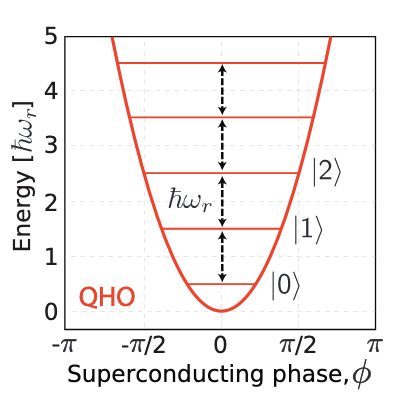
\includegraphics[scale=.8,keepaspectratio]{images/ho-transmon1.jpg}} \qquad \qquad
	\subfloat[][\label{subfig:ho-transmon2}]{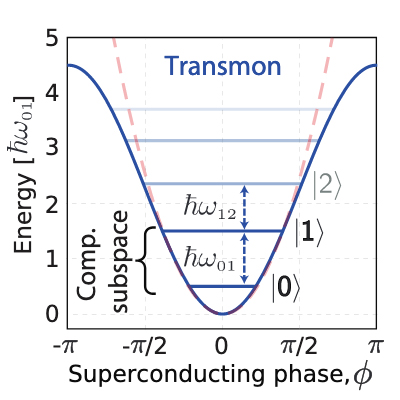
\includegraphics[scale=.8,keepaspectratio]{images/ho-transmon2.jpg}}
	\caption{(\ref{subfig:ho-transmon1}) Spettro energetico del QHO, dove i livelli di energia sono equidistanti l'uno dall'altro. (\ref{subfig:ho-transmon2}) La giunzione Josephson rimodella il potenziale energetico quadratico (tratteggiato in rosso) in sinusoidale (blu fisso), il quale non presenta più livelli energetici equispaziati. Si noti che questo potenziale è una buona approssimazione solamente nel limite $\phi \simeq 0$.}
	\label{fig:ho-transmon}
\end{figure}

\noindent In questa nuova configurazione gli autovalori non sono più equidistanziati: in Figura \ref{fig:energy-difference-transmon} possiamo notare che gli stati $\ket 0$ e $\ket 1$ sono separati da un'energia $\hbar\omega$, mentre gli stati $\ket 1$ e $\ket 2$ da un'energia $\hbar\omega+\alpha$ con $\alpha<0$. (Si veda la discussione che segue per capire perché in figura è indicata la frequenza "$\tilde{\omega}$", non "$\omega$"). 

\begin{figure}[H]
	\centering	
	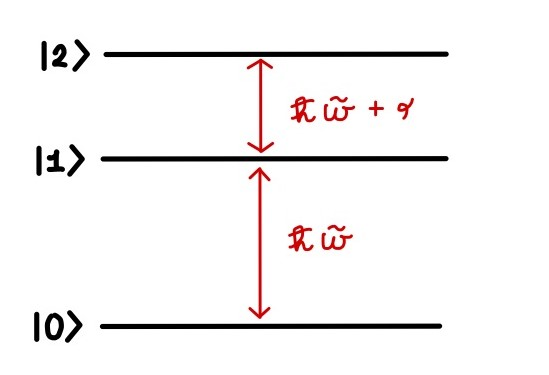
\includegraphics[scale=.45, keepaspectratio]{images/energy-difference-transmon.jpg}
	\caption{Differenza energetica tra i livelli $\ket 0$, $\ket 1$ e $\ket 2$.}
	\label{fig:energy-difference-transmon}
\end{figure}

\noindent Se $\hbar \omega$ è ragionevolmente grande possiamo pensare di utilizzare gli stati $\ket{0}$ e $\ket{1}$ per codificare il qubit e usare degli impulsi laser esterni di frequenza $\sim \omega$ per mandare solamente $\ket{0} \leftrightarrow \ket{1}$, dato che questi livelli non sono in risonanza con tutti gli altri. In particolare, nel caso dei transmon qubit, si lavora con $\omega \sim 3-4 \text{ GHz}$ mentre $\alpha \sim 300 \text{ MHz}$, quindi $E_J/E_C \sim 40$. Tuttavia, a volte, per misure di precisione, si necessita l'utilizzo del livello $\ket 2$, quindi non lo si tiene molto distante energeticamente dagli altri livelli.

\noindent Per vedere esplicitamente come avviene la codifica del qubit, usiamo la definizione di $\hat \phi$ e esplicitiamo gli oscillatori delle relazioni \eqref{Phi_Q_oscill}
\begin{align*}
    \hat \phi = \frac{2\pi}{\Phi_0}\Phi = \frac{2e}{\hbar}\Phi = \frac{2e}{\hbar}\sqrt{\frac{\hbar}{2C\omega}}\left(\hat a + \hat a^\dagger\right) = 2\left(\frac{E_C}{8E_J}\right)^{\frac 14}\left(\hat a + \hat a^\dagger\right) \, ;
\end{align*}
(abbiamo utilizzato le definizioni di $E_C$ e $E_J$). Inserendo questo risultato all'interno dell'hamiltoniana in \eqref{eq:ham-transmon} otteniamo
\begin{equation}\label{H_sviluppare_quartico}
    \hat H = \underbrace{\hbar\omega\left(\hat a^\dagger\hat a+\frac 12\right)}_{\hat{H}_0}-\frac{E_C}{12}\left(\hat a + \hat a^\dagger\right)^4 \, .
\end{equation}

\noindent Questa è un'hamiltoniana di un oscillatore anarmonico con potenziale quartico che non presenta alcuna soluzione analitica. Come al solito, per semplificare la situazione, consideriamo l'hamiltoniana libera, ci mettiamo in un sistema ruotato e teniamo solamente i termini dell'interazione che evolvono lentamente nel tempo. L'operatore che effettua la rotazione è quindi 
\begin{equation*}
    \hat U = e^{i\hat H_0t} \, ,
\end{equation*}
che applicato agli operatori di creazione e distruzione genera una fase dipendente dal tempo (si vedano le relazioni in \eqref{RWA_ops_trans})
\begin{equation*}
    \hat a \longrightarrow e^{-i\omega t}\hat a \qquad \hat a^\dagger \longrightarrow e^{i\omega t}\hat a^\dagger \, .
\end{equation*}
Questo significa che tutti i termini che hanno un differente numero di $\hat{a}$ e $\hat{a}^\dag$ in $\left(\hat a + \hat a^\dagger\right)^4$ sono mediamente nulli; soltanto i termini con un ugual numero sopravvivono, ovvero
\begin{equation*}
    \left(\hat a + \hat a^\dagger\right)^4 = \hat a\hat a\hat a^\dagger\hat a^\dagger+\hat a\hat a^\dagger\hat a\hat a^\dagger+\hat a\hat a^\dagger\hat a^\dagger\hat a+\hat a^\dagger\hat a^\dagger\hat a\hat a+\hat a^\dagger\hat a\hat a\hat a^\dagger+\hat a^\dagger\hat a\hat a^\dagger\hat a \, ;
\end{equation*}
ricordando che $\comm{\hat a}{\hat a^\dagger}=1$ possiamo portare tutti gli $\hat{a}^\dag$ sulla sinistra e scrivere i termini in \textit{normal ordering}
\begin{equation*}
    \left(\hat a + \hat a^\dagger\right)^4 = c_1\hat a^\dagger \hat a^\dagger\hat a \hat a + c_2\hat a^\dagger \hat a + c_3 \, ,
\end{equation*}
dove $c_1=6$, $c_2=12$ e $c_3=3$. Nella nostra trattazione non consideriamo $c_3$ perché comporta solamente una ridefinizione dell'energia di punto zero; il fatto che $c_2$ sia uguale a $12$, come vedremo ora, è importante. Tenendo conto di questo risultato e non considerando i termini costanti, l'hamiltoniana in \eqref{H_sviluppare_quartico} si scrive
\begin{align}
    \hat H &= \hbar\omega\hat a^\dagger \hat a - \frac{E_C}{2}\hat a^\dagger\hat a^\dagger \hat a \hat a - E_C\hat a^\dagger\hat a \notag \\
    \Rightarrow \quad \hat{H} &= \hbar\tilde{\omega}\hat a^\dagger \hat a + \frac{\alpha}{2}\hat a^\dagger \hat a^\dagger \hat a \hat a \, , \label{final_H_transmon}
\end{align}
dove abbiamo posto $\hbar\tilde{\omega}=\hbar\omega-E_C$ lo shift in frequenza del qubit e $\alpha = -E_C$ l'energia del termine quartico. Ricordando come al solito l'azione di $\hat{a}$ e $\hat{a}^\dag$ su $\ket{n}$ dalle relazioni in \eqref{a_adag_action_states}, questa nuova hamiltoniana presenta i seguenti livelli energetici
\begin{align*}
    \hat H \ket 0 &= 0 \, , \\
    \hat H \ket 1 &= \hbar\tilde{\omega} \ket{1} \, , \\
    \hat H \ket 2 &= \left( 2\hbar\tilde{\omega}+\alpha \right) \ket{2} \, ;
\end{align*}
è evidente quindi, come nella Figura \ref{fig:energy-difference-transmon}, che $E_1-E_0 = \hbar \tilde{\omega}$ e $E_2 - E_1 = \hbar \tilde{\omega} + \alpha$. Si noti, in particolare, che $\ket 2$ è ancora autostato, infatti
\begin{align*}
    \hat a^\dagger \hat a^\dagger \hat a \hat a\ket 2 &= \hat a^\dagger \hat a^\dagger \hat a \sqrt 2 \ket 1 = \hat a^\dagger \hat a^\dagger \sqrt 1\sqrt 2 \ket 0 \\
    &= \hat a^\dagger \sqrt 1 \sqrt 1 \sqrt 2 \ket 1 = \sqrt 2 \sqrt 1 \sqrt 1 \sqrt 2 \ket 2 = 2\ket 2 \, .
\end{align*}
Vediamo alcune grandezze tipiche: se il rapporto $E_J/E_C \sim 40$ e $\hbar\omega=\sqrt{8E_CE_J}\sim 10E_C$ allora la differenza energetica $\alpha$ è circa del $10$\%. 

\noindent Ricapitolando, per codificare il qubit l'idea è quella di considerare gli stati $\ket 0$ e $\ket 1$ e trascurare $\ket 2$ (se non utilizzarlo per le considerazioni viste precedentemente). Consideriamo i seguenti stati
\begin{equation*}
    \ket 0 = \begin{pmatrix}1 \\ 0\end{pmatrix} \qquad \ket 1 = \begin{pmatrix}0 \\ 1 \end{pmatrix} \, ,
\end{equation*}
allora in forma matriciale
\begin{equation*}
    \hat a^\dagger \hat a = \begin{pmatrix}0 & 0 \\ 0 & 1\end{pmatrix}=-\frac{\hat \sigma_3}{2}+\frac{\mathbb{I}}{2} \, ;
\end{equation*}
trascurando nuovamente il termine costante si ottiene l'hamiltoniana standard di un sistema a due livelli:
\begin{equation}\label{usual_H_qubit}
    \hat H = -\frac{\hbar}{2}\tilde{\omega}\hat \sigma_3 \, .
\end{equation}
Il termine quartico $\hat a^\dagger \hat a^\dagger \hat a \hat a$ è nullo su $\ket 0$ e $\ket 1$, ma è necessario tenerlo in considerazione quando si vuole includere correzioni dovute allo stato eccitato $\ket 2$.
In un contesto di oscillatore armonico lo spazio di Hilbert considera solamente
\begin{align*}
    \hat a \ket 0 &= 0 \quad &\hat a^\dagger\ket 0 &= \ket 1 \\
    \hat a \ket 1 &= \ket 0 \quad &\hat a^\dagger \ket 1 &= \sqrt 2 \ket 2 \overset{!}{\equiv}0 \, ,
\end{align*}
perché nell'ultimo caso abbiamo troncato lo spazio di Hilbert. Le definizioni matriciali degli operatori di creazione e distruzione possono essere facilmente dedotte dalla forma vettoriale di $\ket{0}$ e $\ket{1}$:
\begin{equation}\label{a_adag_matrices}
    \hat a =\begin{pmatrix}0 & 1 \\ 0 & 0\end{pmatrix} \equiv \hat \sigma_+ \, , \qquad \hat a^\dagger = \begin{pmatrix}0 & 0 \\ 1 & 0\end{pmatrix} \equiv \hat \sigma_-
\end{equation}
In maniera del tutto simile possiamo anche notare che 
\begin{equation}\label{sigma12_aadag}
    \hat \sigma_1=\left(\hat a + \hat a^\dagger\right) \, , \qquad \hat \sigma_2=-i\left(\hat a - \hat a^\dagger\right) \, .
\end{equation}

\noindent Precisiamo che vi sono altre tipologie di transmon qubit: ad esempio, molto diffusi, sono quelli in cui si aggiungono nel circuito di Figura \ref{subfig:J-effect} due giunzioni Josephson in maniera tale che $\tilde{\omega}$ possa essere regolata sperimentalmente mediante una variazione di un flusso magnetico esterno $\phi_e$. Una rappresentazione schematica di questo tipo di qubit è data dalla Figura \ref{fig:split-transmon-qubit}.

\begin{figure}[!ht]
    \centering
    \begin{circuitikz}
        \draw
        (0,0)   to[C=$C$] ++ (0, 3) -- ++ (4,0);
        \draw 
        (2,3)        to[josephson=$L$] ++ (0,-3) -- ++ (-2,0);
        \draw 
        (4,3)        to[josephson=$L$] ++ (0,-3) -- ++ (-2,0)
        (1,0)node[ground]{};
    \end{circuitikz}
    \caption{Transmon qubit caratterizzato da due giunzioni Josephson. La frequenza del qubit è regolata attraverso la variazione di un campo magnetico esterno $\phi_e$.}
    \label{fig:split-transmon-qubit}
\end{figure}
    \begin{thebibliography}{12}
\section*{Corso}
\bibitem{nucciotti}
Nucciotti, A. (2021). \href{https://elearning.unimib.it/course/view.php?id=39133}{Tecnologie Quantistiche Applicate}. Università degli Studi di Milano - Bicocca.
\section*{Libri}
\bibitem{nielsen}
Nielsen, M. A., Chuang, I. L. (2000). Quantum Computation and Quantum Information. Cambridge University Press.
\bibitem{braginsky}
Braginsky, V., Khalili, F., \& Thorne, K. (1992). Quantum Measurement. Cambridge: Cambridge University Press.
\bibitem{schmidt}
Schmidt, V. V. (1997). The Physics of Superconductors. Introduction to Fundamentals and Applications. Springer Berlin, Heidelberg.
\bibitem{tinkham}
Tinkham, M. (2004). Introduction to Superconductivity. Dover Publications.
\bibitem{feynman}
Feynman, R. (2011). The Feynman Lectures on Physics Vol 3 Quantum Mechanics, Chapter 21. Basic Books.
\bibitem{zagoskin}
Zagoskin, A. (2011). Quantum Engineering: Theory and Design of Quantum Coherent Structures. Cambridge: Cambridge University Press.
\bibitem{chen}
Chen, G., Church, D. A., Englert, B.-G., Henkel, C., Rohwedder, B., Scully, M.O., \& Zubairy, M.S. (2006)
Quantum Computing Devices: Principles, Designs, and Analysis (1st ed.). Chapman and Hall/CRC.
\bibitem{devoret}
Devoret, M.H. (1997). Quantum Fluctuations in Electrical Circuits. In Quantum Fluctuations (Les Houches Session LXIII). Elsevier.

\section*{Tesi}
\bibitem{schuster}
Schuster, D. I. (2007). Circuit Quantum Electrodynamics. PhD Thesis, Yale University.
\bibitem{slichter}
Slichter, D. H. (2011). Quantum Jumps and Measurement Backaction in a Superconducting Qubit. PhD Thesis, University of California, Berkeley.
\bibitem{long}
Long, J. (2014). Superconducting Quantum Circuits for Quantum Information Processing. PhD Thesis, Colorado University.

\section*{Articoli}
\bibitem{quantum-noise}
Clerk, A. A., Devoret, M. H., Girvin, S. M., Marquardt, F., \& Schoelkopf, R. J. (2010). Introduction to quantum noise, measurement, and amplification. Reviews of Modern Physics, 82(2), 1155–1208.
\bibitem{quantum-oscillator}
Caves, C. M., Thorne, K. S., Drever, R. W. P., Sandberg, V. D., \& Zimmermann, M. (1980). On the measurement of a weak classical force coupled to a quantum-mechanical oscillator. I. Issues of principle. Rev. Mod. Phys., 52, 341–392.
\bibitem{ql-linear-amp}
Caves, C. M. (1982). Quantum limits on noise in linear amplifiers. Phys. Rev. D, 26, 1817–1839.
\bibitem{sup-qubit1}
Krantz, P., Kjaergaard, M., Yan, F., Orlando, T., Gustavsson, S., \& Oliver, W. (2019). A quantum engineer’s guide to superconducting qubits. Applied Physics Reviews, 6(2), 021318.
\bibitem{sup-qubit2}
Girvin, S. M. (2012). Circuit QED: Superconducting Qubits Coupled to Microwave Photons. Oxford University Press.
\bibitem{jj}
Martinis, J. M., Devoret, M. H., \& Clarke, J. (1987). Experimental tests for the quantum behavior of a macroscopic degree of freedom: The phase difference across a Josephson junction. Phys. Rev. B, 35, 4682–4698.
\bibitem{sc-q-c}
Wendin, G., \& Shumeiko, V. S. (2005). Superconducting Quantum Circuits, Qubits and Computing.
\bibitem{naghiloo}
Naghiloo, M. (2019). Introduction to Experimental Quantum Measurement with Superconducting Qubits.
\bibitem{martinis-1}
Martinis, J. M., Nam, S., Aumentado, J., \& Urbina, C. (2002). Rabi Oscillations in a Large Josephson-Junction Qubit. Phys. Rev. Lett., 89, 117901.
\bibitem{blais-1}
Blais, A., Huang, R.-S., Wallraff, A., Girvin, S. M., \& Schoelkopf, R. J. (2004). Cavity quantum electrodynamics for superconducting electrical circuits: An architecture for quantum computation. Phys. Rev. A, 69, 062320.
\bibitem{koch-1}
Koch, J., Yu, T. M., Gambetta, J., Houck, A. A., Schuster, D. I., Majer, J., \& Schoelkopf, R. J. (2007). Charge-insensitive qubit design derived from the Cooper pair box. Phys. Rev. A, 76, 042319.
\bibitem{walter-1}
Walter, T., Kurpiers, P., Gasparinetti, S., Magnard, P., Potoč, A., Salathé, Y., \& Wallraff, A. (2017). Rapid High-Fidelity Single-Shot Dispersive Readout of Superconducting Qubits. Phys. Rev. Applied, 7, 054020.
\bibitem{dassonneville-1}
Dassonneville, R., Ramos, T., Milchakov, V., Planat, L., Dumur, É., Foroughi, F., \& Buisson, O. (2020). Fast High-Fidelity Quantum Nondemolition Qubit Readout via a Nonperturbative Cross-Kerr Coupling. Phys. Rev. X, 10, 011045.
\end{thebibliography}
    \addcontentsline{toc}{chapter}{Bibliografia}
\end{document}